%%%
%%%
%%% Main TeX File for Lecture Stochastic Simulations in Physics 
%%%
%%%   SS 1998  PD Dr. F. Petruccione  
%%%
%%%
%%% (LaTeX2e Code: P. Biechele) 
%%%
%%%
\documentclass[fleqn,10pt,a4paper,openright]{book}
\NeedsTeXFormat{LaTeX2e}[1996/06/01]
%
% Options:  fleqn     Formulas left not centered
%           leqno     formula numbers to the left, not right
%           openright ????
%
% Create Index
%\usepackage{makeidx}
%\makeindex

%%% USE POSTSCRIPT FONTS (NOT TeX Fonts)
\usepackage{times,helvet,mathptm}

%%% AMS LaTeX Extensions + Fonts 
\usepackage{amssymb}
\usepackage[centertags,intlimits,namelimits,sumlimits,reqno]{amsmath}

%%%%%%%  The graphicx/color style for picture inclusion and color support
\usepackage[dvips]{graphicx,color}
% set path for figures
% more directories can be added by using {dir/} for each
\graphicspath{ {Figures/} }

%%% The Listings package - include source code
\usepackage{listings}

%%% OLD package: 
%%%\selectlisting{java}
%%%\selectlisting{matlab}
% line numbers ? And what stepsize ?
%%% \labelstyle[1]{\ttfamily}
% use small font size for typesetting listings
%%%\prelisting{\small\smallskip\hrule\smallskip}
%%%\postlisting{\smallskip\hrule\smallskip}

%%% NEW package >= V0.19
\lstloadlanguages{Java,Matlab,HTML,TeX}
\lstset{basicstyle=\small, labelstep=5, labelstyle=\ttfamily,
        pre=\small\smallskip\hrule\smallskip,
        post=\smallskip\hrule\smallskip,
        spread=1cm}


%%% SHOW ALL Labels 
\usepackage{showkeys}


% Use extended theorem style
\usepackage{theorem}

%%% The Chapterbib package for Bibliographies per chapter
% TeX usage:  Just insert \bibliography{...bib} where you want to have a bib
%             The style can be given for each bib, but NOT in the main file !
% Compile usage: latex mainfile
%                bibtex chap1
%                bibtex chap2     etc.  (for each chapter)
%                latex mainfile    ! 2 times ! 
\usepackage{chapterbib}

%%%%%%%%%%%%%%%%%%%%%%%%%%%%%%%%%%%%%%%%%%%%%%%%%%%%%%%%%%%%%%%%%%%%%%%%%%%
%%%%%%%%%  END OF IMPORTANT STYLES %%%%%%%%%%%%%%%%%%%%%%%%%%%%%%%%%%%%%%%%
%%%%%%%%%  AND SETTINGS            %%%%%%%%%%%%%%%%%%%%%%%%%%%%%%%%%%%%%%%%
%%%%%%%%%%%%%%%%%%%%%%%%%%%%%%%%%%%%%%%%%%%%%%%%%%%%%%%%%%%%%%%%%%%%%%%%%%%

%%% Example for setting colors to greyscale
%%% 1 ist weiss und 0 ist schwarz
%%%\definecolor{yellow}{gray}{1.00}
%%%\definecolor{red}{gray}{0.02}

%%% Make fancy (our own) headings and footings
\usepackage{fancyhdr}
%%%%%%%%%% Umschalten auf eigene Kopfzeilen !! (fancyheadings Style) %%%%%%%%%
\lhead[\fancyplain{}{\bfseries\thepage}]%
  {\fancyplain{}{\let\uppercase\relax \bfseries\sffamily\rightmark}}
\rhead[\fancyplain{}{\let\uppercase\relax \bfseries\sffamily\leftmark}]%
  {\fancyplain{}{\bfseries\thepage}}
\chead{}
\lfoot{}
\rfoot{}
\cfoot{}
%% Damit das scharfe s auch richtig geschrieben wird und nicht 'SS'
%% kommt von \uppercase\relax von oben ! 
\edef\SS{\ss}

%%%%%% Small Styles :
%%% 
%%%%%%%%%%% calc       : Rechnen mit TeX Groessen
%%% hhline     : verbesserte Linien in Tabellen
%%% array      : verbesserte Tabellenkontrolle
%%% enumerate  : erweiterte enumerate Umgebung
%%% fancybox   : erweiterte Boxen-Umgebungen
%%% moreverb   : erweiterte Umgebungen fuer Listings
%%% multicol   : verbesserte Spalten-Handling
%%%%%%%%%%%%%% floatfig   : Bilder von Text umfliessen lassen (alt)
%%% float      : verbesserte Bilder Umgebung
%%% psfrag     : Text in PS Bildern, durch TeX Fonts ersetzen
%%% exscale    : Skalierung von Mathe Symbolen besser
%%% natbib     : verbessertes Referenzieren 
%%% pifont     : spezielle Listen mit PS Symbolen 
%%% caption2   : Erweiterte Anpassungen der Captions
%%% subfigure  : Mehrere Bilder in einem figure mit eigenen Unterschriften
%%% rotating   : Drehen von Bildern/Tabllen/Sonstigem
%%%%%% picinpar   : Bilder in Text einbinden oder eben Anfangsbuchstaben
%%%%%% !!! Probleme mit AMSTeX und Picinpar --> deshalb wrapfigure !
%%% wrapfigure : Bilder in Text einbinden oder eben Anfangsbuchstaben
%%% ifthen : If Clauses for newcommands
%%%
%% use small captions and boldface caption labels
\usepackage[small,bf]{caption2}
\usepackage{array,rotating,exscale,natbib,subfigure,ifthen,multicol,verbatim}

%%% English Hyphenations and Titles : LOAD AFTER NATBIB
\usepackage[german,english]{babel}

%%%%%%%%%% Definition des Layouts von \cite Befehlen !! (natbib Style) %%%%%%%
\bibpunct{[}{]}{;}{a}{,}{,}

%%%%%%%% Am Ende des Kompilierens, alle benutzten Zusatzfiles ausgeben %%%
\listfiles

%%%%%%%%%%%%%%%%%%%%%%%%%%%%%%%%%%%%%%%%%%%%%%%%%%%%%%%%%%%%%%%%%%%%
%%%%%%%%%%  Here we define our own commands and environements %%%%%%
%%%%%%%%%%%%%%%%%%%%%%%%%%%%%%%%%%%%%%%%%%%%%%%%%%%%%%%%%%%%%%%%%%%%
\newcommand{\bo}[1]{\mathbf{#1}}
\newcommand{\lvec}[1]{\overrightarrow{#1}} 

% Formelnummern: (chapter.section.equation)
%\renewcommand{\theequation}{\thesection.\arabic{equation}}
% equation fuer jeden Section zurueksetzen: 
%\makeatletter
% \@addtoreset{equation}{section}
%\makeatother
%% Mengensymbol C: complex numbers
\newcommand{\setC}{\ensuremath{\mathbf{C}}}
% Symbol fuer relle Zahlen.
\newcommand{\setR}{\ensuremath{\mathbf{R}}}
%% Mittelwert Symbol
\newcommand{\lr}[1]{\left\langle #1 \right\rangle}

%%% Environement for exercises (uses theorem style)
{ \theoremstyle{plain} %% oder {break}
  \theoremheaderfont{\bfseries\scshape}
  \theorembodyfont{\itshape}
\newtheorem{Ex}{Exercise}[chapter] }
%%% Environement for solutions 
\newenvironment{Solution}[1]%
   { \begin{flushleft} \vspace{.5cm} %
     {\Large\textbf{\textsc{Solution to exercise \ref{#1}}}}%
     \end{flushleft} }%
   { \vspace{.3cm} }

%% new listing environments
\newcommand{\inputlisting}[1]{\lstinputlisting{#1}}
\newcommand{\loadlisting}[2]{\subsubsection{Listing of #1} %
  \lstinputlisting{#2}}

%%%%%%%%%%%%%%%%%%%%%%%%%%%%%%%%%%%%%%%%%%%%%%%%%%%%%%%%%%%%%%%%%
%%%
%%% include HTML specials into DVI: HYPERREF PAKET
%%%
%%% Hyperref Package by Sebastian Rahtz

\newcommand{\href}[2]{#2}

%\usepackage[dvips]{hyperref}
%\usepackage[extension=pdf,hyperfigures,hyperindex,%
%baseurl={http://phym1.physik.uni-freiburg.de/\string~frpe/},%
%pdftitle={Manuskript for Stochastic Simulations in Physics},%
%pdfauthor={PD Dr. F. Petruccione, P. Biechele},%
%pdfsubject={Stochastic Simulation},%
%pdfkeywords={Physics,Stochastics,Simulation,Computer},%
%pagebackref,bookmarks,colorlinks,raiselinks,plainpages,dvips]{hyperref}

%%\usepackage{xr}
%%\externaldocument{kap31.dvi}%
%%%[http://phym1.physik.uni-freiburg.de/~hon/manuskript/kap31]

%%%
%%% After Texing, just dvips and then ps2pdf or Acrobat distiller !
%%%
%%%%%%%%%%%%%%%%%%%%%%%%%%%%%%%%%%%%%%%%%%%%%%%%%%%%%%%%%%%%%%%%%%%%%%%%%%%%%%
%%%%%%%%%%%%%%%%%%%%%%%%%%%%%%%%%%%%%%%%%%%%%%%%%%%%%%%%%%%%%%%%%%%%%%%%%%%%%%
%%%%%%%%%%%%%%%%%%%%%%%%%%%%%%%%%%%%%%%%%%%%%%%%%%%%%%%%%%%%%%%%%%%%%%%%%%%%%%
%%%%%%%%%%%%%%%%%%%%%%%%%%%%%%%%%%%%%%%%%%%%%%%%%%%%%%%%%%%%%%%%%%%%%%%%%%%%%%
%%%%%%%%%%%%%%%%%%%%%%%%%%%%%%%%%%%%%%%%%%%%%%%%%%%%%%%%%%%%%%%%%%%%%%%%%%%%%%
%%%%%   Which part should be compiled by TeX
%\includeonly{Chap0,Chap1,Chap2,JavaSummary}
\includeonly{CD_ROM,Chap0,Chap1,Chap2,Chap3,Chap4,Chap5,Chap6,Chap7,Chap8,Chap9,JavaSummary}
%\includeonly{CD_ROM,Chap0,Chap1,Chap2,Chap3,Chap4,Chap5,Chap6,Chap7,Chap8,Chap9,Listings,Solutions}
%%%%%%%%%%%%%%%%%%%%%%%%%%%%%%%%%%%%%%%%%%%%%%%%%%%%%%%%%%%%%%%%%%%%%%%%%%%%%%
%%%%%%%%%%%%%%%%%%%%%%%%%%%%%%%%%%%%%%%%%%%%%%%%%%%%%%%%%%%%%%%%%%%%%%%%%%%%%%
%%%%%%%%%%%%%%%%%%%%%%%%%%%%%%%%%%%%%%%%%%%%%%%%%%%%%%%%%%%%%%%%%%%%%%%%%%%%%%
%%%%%%%%%%%%%%%%%%%%%%%%%%%%%%%%%%%%%%%%%%%%%%%%%%%%%%%%%%%%%%%%%%%%%%%%%%%%%%
%%%%%%%%%%%%%%%%%%%%%%%%%%%%%%%%%%%%%%%%%%%%%%%%%%%%%%%%%%%%%%%%%%%%%%%%%%%%%%

% Over-full v-boxes on even pages are due to the \v{c} in author's name
\vfuzz5pt % Don't report over-full v-boxes if over-edge is small
\hfuzz5pt % Don't report over-full h-boxes if over-edge is small

\begin{document}

% Title and Author
\title{Stochastic Methods for Physics: \\ An introduction}
\author{F. Petruccione and P. Biechele}
\maketitle

% Inhaltsverzeichnis !!!! -- R�mische Seitennummerierung
\pagenumbering{Roman}
\tableofcontents
\clearpage
\listoffigures 
\clearpage
\listoflistings
\clearpage

%%%%%%%%%%%%%%%%%%%%%%%%%%%%%
% The Chapters !!!!  --  Arabic pagenumbering
\pagenumbering{arabic}

%%% Chapter -0 -- CD ROM Explanations
%%%
%%%    Copyright (c)  2002  Peter Biechele, Francesco Petruccione
%%%
%%%    Permission is granted to copy, distribute and/or modify this document
%%%    under the terms of the GNU Free Documentation License, Version 1.1
%%%    or any later version published by the Free Software Foundation;
%%%    with no Invariant Sections, with the Front-Cover Texts being 
%%%    FrontCover.tex (Chapter Front Cover), and with the Back-Cover Texts being BackCover.tex (Chapter Back Cover).
%%%    A copy of the license is included in the section entitled "GNU
%%%    Free Documentation License".
%%%

\chapter*{Instructions for the use of the CD ROM}
Install Toolkit



\setcounter{chapter}{-1}
\lstset{language=java}

%%% Chapter 0 -- Java Intro
\chapter{Short Introduction to Programming in Java}
\selectlisting{java}

%%%%%%%%%%%%%%%%%%%%%%%%%%%%%%%%%%%%%%%%%%%%%%%%%%%%%%%%%%%%%%%%%
\section{Programming in Java}
\label{sec:Programming}


\subsection{General considerations}
\label{sec:General_considerations}
This book is about stochastic simulation methods and their applications to
physical systems. The material is presented at an introductory level. We do 
not assume any prior knowledge on probability theory or on the theory of 
stochastic processes. We assume only the material known from the introductory 
courses in theoretical physics. The style of the presentation will be as 
informal as possible and as precise as necessary.



\subsection{Programming languages -- Why Java ?}
\label{sec:Programming_languages}
It is clear that it is not possible to teach simulation methods without 
performing some numerical experiments in the classroom and that it is 
impossible for the students to learn stochastic simulation methods without 
implementing the algorithms. Therefore, the theory and the corresponding 
algorithms will be presented in a highly interconnected, and, we 
hope, organic way.

In order to stick to this idea it was necessary to choose a programming 
language. The obvious criteria for taking such a decision are
\cite[]{GARCIA}
\begin{enumerate}
\item Efficiency,
\item Understandability,
\item Good graphics,
\item Standard/Portable,
\item Cost,
\item Parallelizability.
\end{enumerate}
The first criterion is of course very important because already simple 
stochastic algorithms require a considerable amount of CPU time.
A secondary aim of the course is to make the student acquainted with a 
programming language ``in action'' so they should learn something 
about a ``good 
programming style'' for real-life problems. Visualization of the results 
obtained allows to understand in a plastic way what is going on physically. So 
the interface between program and visualization tool/graphical output should
be comfortable. Last not least the availability of the program should be
guaranteed. The corresponding compilers should be available at low, in the 
ideal case at no cost to the students for home exercises. Furthermore, they
should be portable on PC with Windows or Linux operating systems, on Macintosh
and on workstations from the UNIX world (IBM AIX, Solaris, SGI Irix, ...).
Since almost all universities do have a high--performance parallel computer 
the language should also allow to demonstrate high--performance parallel 
algorithms.

Because of our background of convinced Fortran users we considered the 
following alternatives: our beloved Fortran, MATLAB, a language which 
is popular in 
the engineering and applied mathematics communities, and Java, the 
"Wunderkind" of software developers and of the Internet community. We have 
not considered C, C++ for the simple reason that we never felt the necessity 
to learn them.

All the languages considered  in some sense satisfy the above criteria. All
are more  or less portable on different platforms (at different expenses), all
allow the use of good visualization tools (at different prices), and, of 
course, all are clean. But not all are equally powerful. 

We checked the power (the efficiency) of the languages considered by the 
following benchmark, which represent the prototype of a stochastic simulation. 
We generated 100 trajectories of a typical one-step stochastic process
and compared the CPU times obtained by different languages. The result
of the benchmarks are summarized in the following table. The listings
of the corresponding programs are listed in the appendix.

\begin{table}[htbp]
  \begin{center}
    \leavevmode
    \begin{tabular}{llp{3cm}|c|c}
      Language & OS & Software & Machine & CPU time \\\hline\hline  
   Fortran & Linux & Nag f90 Compiler & ? & \\\hline
   C       & Linux & GCC & ? & \\\hline
   C++     & Linux & G++ & ? & \\\hline
      Java & Linux & JDK 1.1.5 & Pentium II 333 & 6 sec. \\\hline
           & Linux &           & Pentium 200 MMX & 9 sec. \\\hline
           & Linux &           & Pentium 133 & 17 sec. \\\hline
           & Linux & using JIT TYA & Pentium II 333 & 3 sec.\\\hline
           & Win95 & JDK 1.1.7 using Symantec JIT & Pentium 166 & 7 sec. \\\hline
           & Win95 & JDK 1.1.7 without JIT & Pentium 166 & 17 sec. \\\hline
   Matlab  & Win95 & Matlab 5.1 & Pentium 166 & 330 sec.\\\hline
           & Win95 & Matcom Compiler V3.0 with Borland C++ 5 & Pentium 166 & 70 sec.\\\hline 
   Maple   & Linux & Maple V Rel. 4 & ? & \\\hline
Mathematica& Win95 & Mathematica V3.0 & Pentium 133 & ca. 15 Min. \\\hline
    \end{tabular}
    \caption{Performance comparison for different scenarios and languages.
      The test program is a one-step stochastic process. We create 100
      realizations, $g(n)=0.4n, r(n)=0.5n$. On Windows 95 the JIT from
      Symantec is included and automatically used, when executing programs
      with the java command in the JDK. The TYA JIT for Linux is freely
      available and easy to install.}
    \label{tab:performance}
  \end{center}
\end{table}


Of course, in the above test we have not optimized the algorithm to the 
different platforms. Nevertheless, the table clearly shows that MATLAB is 
very slow. Even the compiled version of MATLAB is slower by a factor of 
about 100 
compared to the Fortran code. This is a good reason to disregard MATLAB!

There is also a compiler called High Performance Java by IBM. It generates
much faster code on an workstations. For a comparison with this
compiler see \cite{HPJ}.

Now we have to decide between Java and Fortran. The argument in favour of 
Java which compensates the slightly slower performance (today!, in future 
this might be different) is its portability and the free availability of the
compiler and of the visualization tools. Java runs on every platform and 
it is available at no cost. 

Last not least, we want to mention another advantage of Java. It seems
\cite[]{bigbucks} that there is  a great need for Java programmers in 
different branches of industry today. This need will be even greater in future 
years. So learning Java, might be a kind of "life insurance" for students of 
physics. It will put them in the position to find a good (programming) job.


%%%%%%%%%%%%%%%%%%%%%%%%%%%%%%%%%%%%%%%%%%%%%%%%%%%%%%%%%%%%%%%%
\subsection{Java}
\label{sec:Java}

We have just seen some good reasons to choose Java as the programming language
for our purposes. Here we want to mention some more technical points, from a 
computational science point of view, in favour of Java.

SUN Microsystems has described Java as follows \cite[]{javanutshell}:
\begin{quote}
Java: A simple, object--oriented, distributed, interpreted, robust, secure,
architecture neutral, portable, high--performance, multi-thread, and dynamic 
language.
\end{quote}
Let us try to understand roughly what is meant by the above adjectives.

Java is simple in the sense that the number of language constructs has been 
kept as small as necessary. For ease of migration from other languages some
basic language elements resemble C or C++. However, some features of these 
languages which were rarely used and which have been considered to be unsafe 
have been omitted. For example, in Java there is no goto statement; instead 
it has labelled break and continue statements. The preprocessor of C has been 
eliminated; the program you write is the program that the compiler sees. In 
Java there are no  operator overloading and no multiple inheritance 
features of C++.
One major simplification is that Java does not have pointers!
In Java memory is managed automatically, so the programmer is not responsible 
for the management  of memory space. In particular Java implements an 
automatic  garbage collector.

Java is an object--oriented language and you do not have to think in a 
procedural--based way, as it is the case in Fortran for example. In order to 
solve problems in Java you have to use the notions of classes and objects. 
Every object has a class that defines its data and the methods that operate 
on these data. Classes are hierarchically arranged. A subclass inherits the 
behaviour of its superclass. A class is the basic unit of compilation
and of the execution in Java. All Java programs are classes.

Java is a distributed language, which simply means that it provides a lot of 
tools for networking. Java is the programming language of the Internet.

Java is an interpreted language. The Java compiler compiles the Java
source code into Java byte--code, which is the machine language for the Java
Virtual Machine (JVM). The JVM is an abstract machine which runs on each system
that supports Java. Other languages may also be compiled into Java byte-code.

Java is robust. Java contains features, exception handling, which simplify the
tasks of error handling and recovery.

Java is secure. Since Java has been designed for distributed applications, 
high security standards have been implemented. For example, direct access to
memory is not allowed. Java contains four different levels of security 
checks and enforcements to prevent the introduction of viruses. 
In particular there is protection against deleting and modifying files.

Java is architecture neutral and portable. The byte-code format is always the 
same regardless of the platform on which the Java compiler runs. Furthermore,
there are no ``implementation defined'' behaviours in Java. For example, Java
specifies the size of each primitive data type. The integer 
types byte, short, int, long are 8, 16, 32 or 64--bit long, respectively.

Java is a high--performance language. 
Usually implementations of Java are used running 
Java programs interpretatively. It is however possible to run Java with a 
Just In Time (JIT) compiler. JIT compiling increases the performance of Java 
considerably.

Java is multi-thread. It supports multiple threads of execution which can 
handle different tasks. Multi-threading increases the interactive performance 
of Java.

Java is dynamic. Any Java class can be loaded into a running Java interpreter 
at any time.

Java includes the zlib compression library in the 1.1. language specification.
These are
the freely available compression libraries used in the well-known
gzip compressor.
That makes it very easy to write and read compressed data. 


%%%%%%%%%%%%%%%%%%%%%%%%%%%%%%%%%%%%%%%%%%%%%%%%%%%%%%%%%%%%%%%%%
\section{Basic elements of Java}
\label{sec:Basic_elements_of_Java}
Like in other languages to write a program you first need an editor
to type the source code. Second you need a compiler to translate
the Java code to byte-code. And last, in contrast to most
traditional languages like C, C++ and Fortran, we need a virtual
machine (interpreter, called JVM) to execute the byte-code.

\begin{figure}[htbp]
  \begin{center}
    \leavevmode
    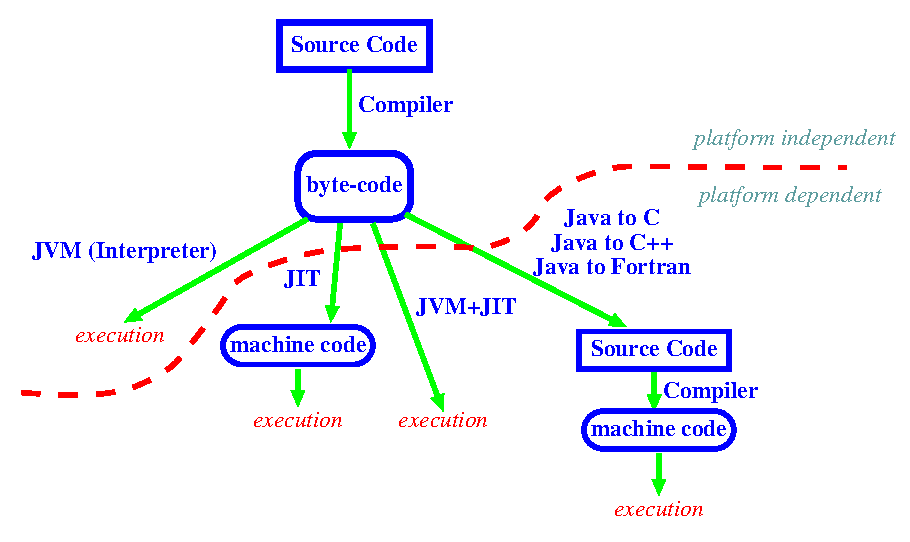
\includegraphics{Figures/Java_Overview.eps}
    \caption{Overview of the Java language execution model.}
    \label{fig:Java_Overview}
  \end{center}
\end{figure}

So for every platform, where a virtual machine is available,
you can execute the byte-code without any compatibility problems.
But the ``look and feel'' can be different, for example Java buttons
in Windows look different from buttons in X11/Motif using a UNIX
operating system. The main reason for the wide availability of Java
is that SUN Microsystems distributes the Java Development Kit (JDK)
freely for a number of important platforms (Windows, Solaris/Linux,
other Unix systems). The JDK consists of a compiler (javac), a
debugger (jdb) and a virtual machine (java)\footnote{Actually there
are some more components like the javadoc command to create HTML
documentation or the jar tool to create zipped packages of
class files belonging together - see later on.}.

The JDK can be downloaded from the internet from the 
\href{http://www.javasoft.com}{JDK Javasoft link page}.
The newest version (as of the time of writing) is 1.1.7. 
There is already a beta version for the JDK
of the new Java 1.2 language specification. Throughout the book,
we will use the Java 1.1 language version and the JDK 1.1.7.

The only additional thing necessary to have a Java programming
environment is an text-editor to write the Java programs. For that
you should use your favorite editor, e.g. emacs or xemacs, which are
also freely available and have nice Java editing modes.

There is also a freely available IDE (Integrated Development 
Environment) called \href{http://www.freebuilder.org/}{FreeBuilder}.
This is a complete environment to write Java programs comfortably,
which is the first under the GNU license. It is still in alpha
development stage, but it already comprises a lot of features. Of
course, there are many commercial ones available, like SUN's Java Workshop.

Opposing to other languages, which use the ASCII character set, Java
uses the Unicode character set \href{http://unicode.org}{(Unicode WWW
Homepage)}. 
Unicode consists of characters represented
by 2 bytes instead of 1 byte like in the ASCII set. So you can not only
use 256 different characters (ASCII) but you can use all the 38885 different
characters available in the Unicode set (Version 2) for writing a Java program.
This means you can name your variables using for example Japanese or Greek
characters. Right from the beginning, Java is an international language.

Java is also case sensitive and doesn't need any special characters
to mark continuation lines. 

Comments are used just like in C and C++.
You can use either the /* \ldots */ syntax (borrowed from C) for
multi-line comments or the // syntax (borrowed from C++) for single
line comments. Additionally you can use /** \ldots */ for comments
to automatically generate a HTML documentation file for the class
defined in the file. We will see later on how zhis can be achieved.
 
\subsection{The ``HelloWorld'' Program}
\label{sec:HelloWorld}
Now let's start with the traditional ``Hello World'' program written
in Java.

\subsubsection{Application}

\inputlisting{Listings_Java/HelloWorld_Application.java}
You have to save the program in a file called 
\verb|HelloWorld_Application.java|.
To execute the above example you have to type in the commando line the
following:
\begin{itemize}
\item Compiler: \verb/javac HelloWorld_Application.java/  
  $\Longrightarrow$ produces HelloWorld\_Application.class 
  in the same directory.
\item JVM:  \verb/java HelloWorld_Application/
\item Output on screen: \verb<Hello World !<
\end{itemize}
Let us now try to understand the above code. The program consists of
three lines. 

In the first line the program declares 
with the help of the \texttt{class} statement a class called 
\verb|HelloWorld_Application|. 
The identifier following the \texttt{class} statement is
the name by which the class will be referenced. Each Java program
is a class. The curly bracket appearing after the class name
\verb|HelloWorld_Application| introduces the following class member. 


In the second line the \verb|main| method is introduced. The main
method is declared \verb|void| because the method does not return a
value. The main method is executed when you run the class as an
application. In the present case the only parameter, the argument
of the main method, is an array of String object.

In the third line the method \verb|println| of the system class out
is invoked. This method simply prints a string and terminates with a 
new--line  command.

You have just written and executed your first application in
Java. Please, do not worry if you do not undestand everything. You are
not expected to understand everything at this stage.


\subsubsection{Applet}
\label{sec:Applet}

Java offers another possibility to execute code, so called Applets.
In contrast to the stand--alone Java application which starts at
\verb!main! and runs until it is completed, the applet is a kind of
sub--program which runs under the control of some other program.
Usually, applets are (small) Java programs, which are started by a 
server program,
e.g. a WWW browser like Netscape Navigator\footnote{You need at least 
version 4.06 or patches for earlier versions to use all features of Java 1.1}, 
the Internet Explorer\footnote{Seems to run Java 1.1 programs since
version 4.}(Don't),
HotJava or the appletviewer\footnote{included with the JDK.}.

The big difference between an applet and an application is that
applets are not allowed to do certain things. For example applets
do not have access to local file systems, so it is not possible
to save data on the file system from an applet. It is also not
possible for an applet to issue a print command, the process of
printing has to be initiated by the server (browser). 
And an applet is not allowed to do time consuming tasks like
long computations. This has to be kept in mind, when writing
applets.


The ``Hello World'' example written as an applet has the following form:
\inputlisting{Listings_Java/HelloWorld_Applet.java}

Applets have to be derived from the applet class
\verb|java.applet.Applet|, which include the principal facilities of
the Abstract Window toolkit (AWT) and the interface with X/Motif on
Unix, Windows on PC, and MacOS on Macintosh platforms.
As you can see there is no main method in an applet. Instead if an applet
is started by a server, the init() method is executed first. There is also
a start() (stop()) method, which is executed if the applet becomes
visible (disappears) in the server window (e.g. by scrolling in the
Netscape Navigator window).

Many methods are available to set up the display in an assigned applet area.
The paint() method appearing in the ``Hello World'' applet is
responsible for the visual part of the applet. It uses a canvas
(drawing area) with a size defined by the calling HTML file. In our case
this HTML file could look like:
\inputlisting{./Listings_Java/call_HelloWorld_Applet.html}
The code parameter given in the HTML file defines the name of the applet
to be run. Because there is no init() and no start() method in our
example, the paint() method gets executed by the browser (or appletviewer).
The size of the canvas has to be given in pixels explicitly in the
HTML file.

To run the applet you can either type
\begin{itemize}
\item \verb|appletviewer  call_HelloWorld_Applet.html| or
\item use the following URL in the browser: \\
        \verb|PATH_TO_CLASS_AND_HTML_FILE/call_HelloWorld_Applet.html| \\
        e.g. \verb|/home/user/java/call_HelloWorld_Applet.html|
\end{itemize}

The question arising now, when to use an application and when to use
an applet, is difficult to answer. In the following chapters we will 
decide for each program
separately, which way to go. Time consuming calculations should
definitly be written as an application, small programs can be
written as an applet of course.

A last remark concerns the documentation for the programs. We have
learned, that we can include documentation comments using 
\verb|/** .... */|. These comments are processed by using the
\verb|javadoc| command from the JDK. If you run the javadoc command as: 
\begin{verbatim}
  javadoc HelloWorld_Application.java HelloWorld_Applet.java  
\end{verbatim}
you get some HTML files: packages.html, tree.html, AllNames.html,
HelloWorld\_Applet.html, HelloWorld\_Application.html. All these
files describe the written classes. The tree.html gives a tree
showing the relatives of the class. The package.html gives the
package structure (not used here). The most important file is the
AllNames.html, which is an index of all written programs in this package
(for an introduction to packages see later).

If you load AllNames.html into a browser, you get:
\begin{center}
 \includegraphics[width=5cm]{Listings_Java/AllNames.eps} 
\end{center}
Now you can klick on the link HelloWorld\_Applet and you get the
documentation for that class:
\begin{center}
  \includegraphics[width=5cm]{Listings_Java/HelloWorld_Applet.eps}
\end{center}
and for the HelloWorld\_Application you get:
\begin{center}
  \includegraphics[width=5cm]{Listings_Java/HelloWorld_Application.eps}
\end{center}
The missing graphics is available in the Java documentation of the
JDK and just has to be copied into the HTML directory.

%%%%%%%%%%%%%%%%%%%%%%%%%%%%%%%%%%%%%%%%%%%%%%%%%%%%%%%%
\subsection{Variables}
\label{sec:Variables}

Essentially, Java distinguishes between two types of variables,
primitive data types and reference data types.
\subsubsection{Primitive data types}
\label{sec:primitive_data_types}
We already mentioned that in Java each variable or expression has a
definite type and that each type has identical size and behaviour on
all Java implementations.  Java has built in primitive data types
to support integer, floating--point, boolean, and character values.
The primitive data types of Java for integers, floating--points,
characters and boolean variables are listed in table
\ref{table:primitivedata}.
\begin{table}[htbp]
\label{table:primitivedata}
\begin{center}
\begin{tabular}{l|l|l|l|l|l}
Type & Contains & Default & Size & Min \\
     &          &         &      & Max \\ \hline \hline
byte  & signed integer & 0 & 8bits & -128  \\
&&& & 127    \\ \hline
short & signed integer & 0 & 16 bit &-32768 \\
&&& & 32767 \\ \hline
int &   signed integer & 0 & 32 bits&-2147483648 \\
&&& &2147483647 \\ \hline
long & signed integer & 0 & 64 bits &-9223372036854775808\\
&&& &9223372036854775807\\ \hline
float & floating--point & 0.0 & 32 bits &$\pm$1.40239846E-45\\
&&& &$\pm$3.40282347E+38\\ \hline
double & floating--point & 0.0 & 64 bits &$\pm$4.94065645841246544E-324\\
&&& &$\pm$1.79769313486231570E+308\\ \hline
boolean & true or false      &  false & 1 bit&\\
&&&       &  \\ \hline
char  & Unicode character & $\backslash$u000 & 16 bits & $\backslash$u000 \\
&&& &$\backslash$uFFFF   \\ \hline
\end{tabular}
\end{center}
\caption{Primitive data types in Java.}
\end{table}


The following comments have to be done. In a Java program every
variable must have a type that precedes its name when the variable is
declared. For example the integer i may be declared as

\begin{verbatim}
int i;
\end{verbatim}


Char values represent characters. They appear in Java between single
quotes, e.g.
\begin{verbatim}
char c = 'C';
\end{verbatim}
A Unicode character is represented by the Unicode escape sequence
$\backslash$uxxxx, where xxxx is a sequence of four hexadecimal digits.


Float and double types have special values that may be the result of
certain floating-point operations. For example in the java.lang.Float
and java.lang.Double classes the special values
\verb|POSITIVE_INFINITY|, \verb|NEGATIVE_INFINITY|, and 
\verb|NaN| (not-a-number) are
defined.

Floating point numbers are expressed as e.g.
\begin{verbatim}
13.       1.3e1        .13E2 
\end{verbatim}
and are considered to be constants of type \verb|double| 
unless they are specified with \verb|f| or \verb|F|, which makes them
then \verb|float| constants.

In Java strings are not a primitive type. Java provides a String
class to deal with sequences of character data. The java string
class provides methods to operate on String objects.

All variables in Java are initialized automatically, as soon as they
are declared. All primitive types get initialized to zero, the boolean type
to false and all objects (remember they are references) are initialized
to \verb|null|. So there is no ambiguity like in other languages, if
a variable has a defined value at certain points of the program. 
Although Java forces you to include sometimes a statement to
initialize variables, just to make easier to read source code.
We will see an example for this later on, when we discuss loops
and calculate averages of sequences of numbers.

\subsubsection{Reference data types}
\label{sec:Reference_data_types}

All non-primitive data types in Java are objects and arrays. They are
called also ``reference types'' because they are handled by
reference. For example you may pass the address of an object, which is
stored in a variable, to a method. In contrast, primitive types are
always passed by value.


%%%%%%%%%%%%%%%%%%%%%%%%%%%%%%%%%%%%%%%%%%%%
\subsection{Casting, Wrapper Classes}

Java uses a clear strategy to convert the primitive data types to 
other primitive ones. In a calculation Java always converts (casts)
the less precise type to a more precise one. So if you multiply an
integer and a float value, it converts automatically the integer to
a float and then multiplies both values. If you want to convert
a value explicitly you can use the cast operators (like in C and C++).
Just write the primitive type in round brackets in front of the value to
be converted, e.g. \verb|result=(double)a*b| casts \verb|a| to 
a double value and
then multiplies it with \verb|b|, assigning the result to \verb|result|.

A common problem is to convert from strings to primitive types and
vice versa. Because strings are objects and not primitive types, we
need a method for the conversion. For that reason Java has so called
wrapper classes in \verb|Java.lang| for all the primitive types. 
These classes provide all the necessary methods for all types of
conversion. The \verb|valueOf()| method always converts a string
to the corresponding wrapper class of a primitive type, e.g. 
\begin{verbatim}
        double a;
        String text;
        a=doubleValue(text.valueOf());
\end{verbatim}
The third line converts the string to the \verb|Double| class and then
the \verb|doubleValue()| method converts to a double primitive type.
For the other types you just have to substitute float or int 
for double.
 
Another method, later used in the \verb|ParamApplet.java| program is
the \verb|Integer.parseInt()| method, which gives back a primitive
type integer instead of the wrapper class like \verb|valueOf()|.
This simplifies the conversion a little bit. For the example, see
\verb|ParamApplet.java| in line 11. But this method is only 
available to Integer, Long and Byte wrapper classes, NOT for
Float and Double. In this case you have to use the \verb|valueOf()| and
\verb|doubleValue()|, \verb|floatValue()| methods.

To convert a double value to a string you have to use the \verb|toString()|
method, which is available for all primitive data types. 



%%%%%%%%%%%%%%%%%%%%%%%%%%%%%%%%%%%%%%%%%%
\subsection{package and import statements}
Because Java was designed to be able to load code distributed
over the whole internet, you have to avoid name conflicts
between the programs (classes). The solution in Java is to put
every class in a \emph{package}. The name of the package is given
at the beginning of a file before the actual program (class)
definition starts. So for example if we put the statement
\begin{quotation}
  \verb/ package de.freiburg.simulation; / 
\end{quotation}
at the beginning of the ``Hello World'' application, we can compile
the application with \verb/javac HelloWorld_Application.java / like before.
But to run the application we have to use
\begin{quotation}
  \verb/ java de.freiburg.simulation.HelloWorld_Application / . 
\end{quotation}
You are wondering why the program does not start? It cannot, because
there is one more thing to know. Java is looking for programs (classes)
in the directory structure given by the class name. So
for the example above you have to put the \verb/HelloWorld_Application.class/ file
in the directory \verb|de/freiburg/simulation/| and issue the command
in the directory, where the directory tree starts.

You could also use an environment variable called \verb|CLASSPATH|. It
describes the directories to search for the class files. So if the
\verb|CLASSPATH|-variable includes \verb|/home/user/java| you can
start the above example in this directory, if the class is in the 
subdirectory  \verb|de/freiburg/simulation/|.

All the standard commands (classes) of Java are stored in a central jar
file, which is additionally packed to save disk space. These classes
are always searched, no matter the \verb|CLASSPATH|-variable is set to.

If you are not using the package command at all, Java uses the empty 
package. This means you can put your programs in the current directory.
This is not recommended for medium to complex programs, but for
test purposes and very small programs this is very convenient.



Before learning more about the syntax of Java, we have to explain another
statement appearing in the part of any Java program before the actual
definition of the class: the \verb|import|-statement. With \verb|import|
you can make classes available, so you don't have to use the fully
qualified name to the class. So if you would like to
use the HelloWorld class from above in your programs, you could either
type \verb|de.freiburg.simulation.HelloWorld()| in your program
or you can use
\begin{verbatim}
import de.freiburg.simulation.*;
....
   HelloWorld();
\end{verbatim}
to import all classes in the \verb|de.freiburg.simulation| class.
You can also use:
\begin{verbatim}
import de.freiburg.simulation.HelloWorld;
....
   HelloWorld();
\end{verbatim}
if you just want to import one special class.

We have already made use of the \verb|import|-statement in the ``Hello World'' 
applet. There we have imported the \verb|java.applet|-class, which
defines applets and their behaviour, and the \verb|java.awt|-class, which
will be explained later.
 
There is one class, which is always imported without any import statement:
the java.lang class. This is the fundamental class of Java and it is
implicitly imported for all Java programs, so you do not have to specify
it. For example the System class is in Java.lang, that is why
we did not have to use an import statement in the ``Hello World''
application.  


%%%%%%%%%%%%%%%%%%%%%%%%%%%%%%%%%%%%%%%%%%
\subsection{Simple arithmetics, Conditional Statements and Loops}
\label{sec:Loops}

\subsubsection{Simple arithmetics}
As we already mentioned Java  supports almost all of the standard
C operators. The arithmetic operators that operate on numerical types
are 
\begin{center}
\begin{tabular}{ll}
$+$ & addition \\
$-$ & subtraction                 \\
$*$ & multiplication \\
$/$ & division \\
\% & remainder
\end{tabular}
\end{center}
The $+$ operator can also be used to concatenate strings, as we will
see later in an example in section \ref{sec:Parameter}.

It is important to remark, that in Java integer division truncates
toward zero (7/2=3, -7/2=-3 and -7/-2=3).

Java has two special operators for increment $++$ and decrement $--$. The 
expression \verb|i++| is equivalent to \verb|i=i+1| except that
\verb|i| is evaluated only once. They can be used as pre- and post-operators,
depending on the position of the symbols, e.g. \verb|i++| or \verb|++i|.
This does not make a difference, if you just have these statements
alone, but in some complex expressions this might make a difference.

Java supports also a standard set of relational and logical operators,
which all yield boolean values. They are listed below

\begin{center}
\begin{tabular}{ll}
$>$  & greater than \\
$>=$ & greater than or equal to \\
$<$  & less then \\
$<=$ & less than or equal to \\
$==$ & equal to \\
$!=$ & not equal to
\end{tabular}
\end{center}


The conditional operators
\begin{center}
\begin{tabular}{ll}
\& \& & conditional AND      \\
$\mid\mid$ & conditional OR
\end{tabular}
\end{center}
operate on  boolean expressions only.

Java has also bitwise operators which operate on integers and on
boolean types
\begin{center}
\begin{tabular}{ll}
\& & and \\
$\mid$ & or \\
$\tilde{}$ & not \\
$<<$ &  shifts bits left filling with zero bits on the right \\
$>>$ & shifts bits right filling with the highest sign bit on the
           left--hand side \\
$ >>>$ & shifts bits right filling with zero bits on the left--hand side 
\end{tabular}
\end{center}

Last not least we have to mention the fundamental assignment operator
$=$. It may be used in combination with other operators, e.g., $+=$
means is incremented by.


\subsubsection{Loops}
\paragraph{for Loops}
For our forthcoming applications the most important control statement
is the \verb|for| statement. It is used to loop over a range of values
from the beginning to the end. Its syntax is
\begin{verbatim}
for (init_expressions; boolean_expr; incr_expressions) {
    statements
}
\end{verbatim}
where \verb|init_expressions| denotes the initial value of the iterated
variable, \verb|incr_expressions| denotes the increment of the iterated
variable. For both you can specify more than one expression separated
by commas ( as in C). This is the only place, where you can use these comma
separated lists.

At the beginning of the \verb|for| loop the boolean expression
\verb|boolean_expr| is evaluated. If its value is found to be 
\verb|true| the statement is executed repeatidly with increment
\verb|incr_expr| until the value of the boolean expression is found to
be \verb|false|.

As an example demonstrating the use of
\verb|for| loops we want to write a program to calculate the mean of
a given number of random numbers. One posible implementation
could look like this:
\inputlisting{Listings_Java/DataMean.java}

Here we used the class \verb|java.util.Random| which allows for
the creation of random numbers. If we don't supply a seed, as is the
case here, it just uses the time to initialize the generator. The
initialization takes place in line 10, where a new generator is created.
You can check this by running the application more than once and comparing
the means -- they should not be the same. 

The \verb|next.Double()| method returns a new random number of type
double (for a float use rand.Float()). You can also create normally 
distributed random numbers with the \verb|Random.nextGaussian()| method.
The remaining parts of the program should be self explaining.


\paragraph{while and do--while}
Java offers also the possibility to use other loop constructs, the
\verb|while| and the \verb|do-while| loop. There syntax is
\begin{verbatim}
while (boolean_expression)
 statement
\end{verbatim}
and
\begin{verbatim}
do
  statement
while (boolean_expression)
\end{verbatim}
It is important to observe that in the first construct the boolean
expression is evaluated \textit{before} the statement is exectuted, while in
the second construct the boolean expression is evaluated \textit{after} the
statement has been performed!

In order too give an example we write down an equivalent code using
the
\verb|while| statement of the \verb|for| loop of the
\verb|DataMean.java| program. Lines 13 to 15 have to be replaced by
\begin{verbatim}
int i;
while(i<N){
  mean += rand.nextDouble();
  i++;
}
\end{verbatim}

\subsubsection{Conditional Statements}
\paragraph{if-else}
The \verb|if| statement is the fundamental form of conditional control
of flow. It allows to choose, whether the statements that follow it are
executed or not. Its syntax in Java is
\begin{verbatim}
if (boolean_expression) {
   statement1
}
else if (boolean_expression) {
   statement2
}
else {
   statement3
}
\end{verbatim}
First, the boolean expression is executed. If the value is \verb|true|
then \verb|statement1| is performed, otherwise if there is the
optional \verb|else| statement \verb|statement2| is executed. Of
course, \verb|if-else| constructions can be nested, i.e., an
\verb|if-else| conditional control flow, can be placed within another
\verb|if-else| statement.

\paragraph{goto}
We already remarked that Java does not have a \verb|goto| instruction
to transfer control to an arbitrary statement in a method. To handle
with situations where other languages have a \verb|goto| Java provides
the labelled \verb|break| and \verb|continue| statements. Labels are
typically used in blocks and loops and preced statements
\begin{verbatim}
label: statement
\end{verbatim}
The \verb|break| statement is used to exit from a block, e.g. to break
out of a loop. E.g., an unlabeld \verb|break| terminates the innermost
\verb|for|, \verb|while| or \verb|do|.

The \verb|continue| statement is used only within loops. It skips to
the end of the loop's body and evaluates the boolean expression that
controls the loop. The \verb|return| statement terminates execution of
a method and returns to the invoker. If a method returns no value you
have to use
\begin{verbatim}
return;
\end{verbatim}
if the method has a return type, the \verb|return| must include an
expression for a retuned type.

An dieser stelle sollten einige beispiele kommen!!!!!

\paragraph{switch/case}

Another central flow structure is the \verb|switch| statement. It
evaluates an integer expression whose value is used to find an
appropriate \verb|case| label among those listed inside the following
block. The \verb|switch| statement may be used to replace nested \verb|if-else|
statements that determine what is the output for each number. The
\verb|switch| statement works only if the value being tested is a
primitive integral type and when the value is tested against constant
values. the basic syntax of the \verb|switch| statement is
\begin{verbatim}
switch(expression) {
    statements
}
\end{verbatim}
After evaluating the expression, the switch statement executes
certain code within the block depending on the integral value of the
expression. This information is indicated by the integer label follwing
the \verb|case:| statement. If there is no \verb|case:| label that
matches the value of the expression, the \verb|swich| command executes
the code following \verb|default:|, if there is one. Otherwise,
\verb|switch| does nothing.

An example of the use of the \verb|switch| statement is found in the
simple program \verb|DiceGame.java| 

%\inputlisting{Listings_Java/DiceGame.java}

Ich habe leider das .class Programm auf Diskette! Brine ich morgen mit.
 
%%%%%%%%%%%%%%%%%%%%%%%%%%%%%%%%%%%%%%%%%%%
\subsection{Parameters from the command line or from a html file}
\label{sec:Parameters}

The access of parameters given on the command line is as easy as it
is in C and C++. The parameters are stored as strings in Java and
are given as the parameters to the main() method of the application.
That is the reason for the Syntax:
\begin{quotation}
  \verb|public void main(String[] args) |
\end{quotation}
It means that the array \verb|args| (see section \ref{sec:Arrays}
for an explanation of arrays) contains the parameters. Each parameter
is separated with a space in the command line. Here is an example of a 
program using command line parameters:
\inputlisting{Listings_Java/ParamCommandLine.java}
So if you run the program as \verb|java ParamCommandLine 12 34 abcd t5|
the output on the screen will be
\begin{verbatim}
 Parameter No. 0 : 12
 Parameter No. 1 : 34
 Parameter No. 2 : abcd
 Parameter No. 3 : t5
\end{verbatim}
and if you don't supply parameters it will be
\begin{verbatim}
 NO parameters specified !
\end{verbatim}
We also see the concatenation of strings in the output statement.
And because you can only supply one argument to the  \verb|println()|
method, you have to concatenate all outputs to one long string.

A little bit different is the behaviour of applets, because there is
no command line. But there is also a way to transmit parameters from 
the calling HTML file to the Java applet. In the HTML file you can
specify \verb|<PARAM>| attributes like here:
\inputlisting{Listings_Java/ParamApplet.html}

In this case we supply two parameters, called \verb|NumberofPoints| and
\verb|DisplayText| to the Java applet. The value is given in the string
behind the keyword \verb|value|. The Java applet to this HTML file
could look like this:
\inputlisting{Listings_Java/ParamApplet.java}

In the \verb|init()| method we get the parameter \verb|NumberofPoints|
and convert it to an integer using a wrapper method. The string 
of the parameter \verb|DisplayText| doesn't have
to be converted. Then in the \verb|paint()| method we display
the transmitted parameters on the screen. The output in the 
appletviewer or in Netscape should look like this:
\begin{verbatim}
  Parameter NumberofPoints is 10000

  Parameter DisplayText is "This_is_a_test_parameter!"
\end{verbatim}

%%%%%%%%%%%%%%%%%%%%%%%%%%%

\subsection{Arrays}
\label{sec:Arrays}

Before discussing the notion of classes and objects, we want to introduce
another reference type: the array. They are actually objects, but
Java provides many special commands for arrays, which makes them a 
little bit special.

The first question is how to create arrays and how to destroy them.
The destruction is easy to explain: it is done automatically
by the garbage collector (like for all objects). This is different to
other languages like C, C++ and Fortran 90, where you explicitly
have to destroy (free) the allocated memory. 

To create an array you have to use the \verb|new| keyword used for
creating (instantiating) objects. So to create a one dimensional
array with 10 elements you use:
\begin{verbatim}
        int intarray[] = new int[10];
\end{verbatim}
This also sets all the elements to zero. But this is only true for 
primitive types. Arrays of reference types (objects) are created the
same way, but the elements consist of references to the elements. The
elements themselve are NOT initialized and have to be created too.
An example for this is a two dimensional array as we will see soon.

Indices of arrays in Java start with zero as in C and not with 1
as in Fortran. No negative indices are allowed in Java. The length
of an array (meaning the number of elements) is always given
by the \verb|.length| field. For the array above you get the number
of elements by using \verb|intarray.length|. We have already met
this notation when we discussed the command line parameters.

You can also create the array and initialize it right away by using
(also in Java 1.0):
\begin{verbatim}
        int intarray[] = {1, 2, 3, 4, 5, 6, 7, 8, 9, 10};
        int[] intarray = {1, 2, 3, 4, 5, 6, 7, 8, 9, 10};
\end{verbatim}
or one step further, create an array of objects (here strings) and
create the elements in the same step:
\begin{verbatim}
        String stringarray[] = {"a","b","c","d","e","f","g"};
\end{verbatim}
In Java you can even put the brackets behind the type instead of the
variable name (not possible in C). So it does not matter if you
write \verb|int intarray[];| or \verb|int[] intarray;|.

In Java 1.1 you can also use \emph{anonymous arrays}:
\begin{verbatim}
        String[] texts;
        texts = new String[] = {"a","b","c","d","e","f","g"};
        System.out.println(new char[] {'h','e','l','l','o'});
\end{verbatim}
So you can create and initialize arrays without even using a variable.

Multidimensional arrays are also supported. Just like in C they are
arrays of arrays. For example
\begin{verbatim}
        double matrix[][] = new double[10][10]; 
\end{verbatim}
creates a 10 by 10 matrix, meaning that you have created 10 arrays
of type \verb|double[10]|. An important point to make is that you
do not have to specify all dimensions at once. You can for example
create a triangular matrix by submitting:
\begin{verbatim}
        double matrix[][] = new double[10][];
        for (int i=0; i<10; i++) {
                matrix[i] = new double[i+1];
        } 
\end{verbatim}
To access multidimenisonal arrays you can also use one dimensional
array syntax (as in C). If you have a two dimensional array 
you can access the element [i,j] by accessing the element [i+j*columns]. 

Now let's look at an example using arrays. We have rewritten the program
\verb|DataMean| above to calculate the average of random 
numbers by using arrays.

\inputlisting{Listings_Java/DataMean_Array.java}

Here we first declare a double array called \verb|RandomNumber| and
create it in Line 13. Then we store the random numbers in the array
and afterwards calculate the mean.

The last important point to note is the copying of arrays. 
You can not just write
\begin{verbatim}
        int[] array1 = new int[] = {1,2,3,4,5};
        int[] array2 = new int[10];
        array2 = array1;                // WRONG ! - ERROR ! 
\end{verbatim}
This would only copy the reference of the array1 object to the array2
object, not the values. To copy arrays you have to use the 
\verb|arraycopy()| method of the java.lang.System class. 
So to copy an array in the above example, you have to write:
\begin{verbatim}
        System.arraycopy(array1,0,array2,0,array1.length);
\end{verbatim}
This copies all elements of array1 to array2 staring from element 0. 
The remaining parts 
of array2 is not created!



%%%%%%%%%%%%%%%%%%%%%%%%%%%
\subsection{Classes and Objects}
\label{sec:Classes_and_Objects}

The biggest step you have to take in mastering Java if you are
coming from the Fortran or C community, is to switch to the object
oriented paradigm. Although C++ programmers are used to objects, there
are quite a number of differences to C++ in Java. That is why Java
is closer to C than to C++.

We have already met a lot of object oriented features 
without discussing them in detail. 
\begin{quote}
A class is a collection of data and methods that operate on that data. In
Fortran or C we call the methods procedures or functions. An object
is an instance of the class, meaning it is a thing to work with. The class
defines the data necessary for the object and the functions which can
operate on them.   
\end{quote}
For example you can have a class ``Car'', which describes all the 
eigenschaften of a car, e.g. type, age, weight, etc. Then you have a
``real'' car, let's say a Ford, 10 years old, 1000 kg, etc. So this
is an object of the class ``Car''. A method would be the calculation
of the monthly cost for the car. 

An example already familiar to us, is an array. If you have an array 
object you can call the method \verb|length| to get the number of
elements of the array. 

So what is the difference to the standard function approach here?
Instead of using function arguments you supply the argument by 
putting them in front of the method separated by a point. 
For example to calulate the mean of an array of doubles, you can
either write a method which takes the array as an argument (like you would
in Fortran or C): \verb|mean(array[])| or you can use the object
oriented feature: 
\begin{verbatim}
        Data dat = new Data(); 
        result = dat.mean();
\end{verbatim}
It is up to you, which version you prefer. But because all programs are
actually classes in Java you have to understand at least the 
most fundamental things about object oriented programming. For a detailed
discussion and introduction, see \cite{javanutshell}.

Just to remind you again, strings are objects and not primitive 
types. To use strings you first have to declare and instantiate a string
object. Here are three possible ways of doing it:
\begin{verbatim}
        String text;
        text = "Test String";
        text = new String();
        text = new String("Test String");
\end{verbatim}
The first line only declares a string object called text and does not
allocate (instantiate) the memory for the value of the object, just
the reference to the value.

As an example for the most important issues about objects, we want to
write a class, which calculates random numbers by different methods and
for different distributions. To that end we write a class 
\verb|RandomNumber|. It has three fields (variables), two of them are
defined with the \verb|final| keyword. This is the equivalent to the
const keyword in C. A final field can not be changed anymore.
The \verb|static| modifier defines a field (variable), which is belonging
to the class and not to the object. So every object of that class 
has the same value for a \verb|static| field. The \verb|public| modifier
on the other hand defines a field or method, which is special to 
an object not to the class -- this is also called an instance field or
method, the \verb|static| version is called a class variable or method.
\begin{table}[htbp]
  \begin{center}
    \leavevmode
    \begin{tabular}{l|p{8cm}}
     Modifiers &                                 \\ \hline \hline
     final & variables may not be changed, classes may not be 
                                   subclassed\\\hline
     public & accessible from anywhere\\ \hline
     static & defines a top-level class, a class variable (field) or 
                 a class method\\\hline
     private & only within the defining class visible, not in other 
               packages, even if subclass of this class\\\hline
     protected & accessible within the package in which it is defined and
                 within subclasses\\\hline
     (none) & accessible only in its package\\
    \end{tabular}
    \caption{Overview of some available modifiers in Java. For a complete
      overview take a look at page 230-234 in \cite{javanutshell}.}
    \label{tab:modifiers}
  \end{center}
\end{table}

\inputlisting{Listings_Java/RandomNumber.java}
Class variables and methods are the closest relatives to global 
variables in all the other languages. They are accessible from all
classes, but still are belonging to a class. So you could have two
class methods with the same name, but for different classes.

An important part of any class is the constructor of the class. This is
the method (function), which is called when an object of this
class is instantiated. Here in our example, we just set the seed. As 
you can see you have to supply the seed, when instantiating the
generator. Most of the constructors don't even need a parameter to 
instantiate the object. 

Then the method \verb|nextRand()| is defined and returns the next
random calculated using a congruential method (see later in this
book). The return type of methods always has to be specified, if
there is no return value you have to use the \verb|void| statement
(as in C). The value to be returned is specified by the return keyword.

Now we have to write a program (class), which uses this class to 
calculate the average of some random numbers.
\inputlisting{Listings_Java/UseRandomNumber.java}
The class is called \verb|UseRandomNumber| and just contains the
main method. First we instantiate (create) an object of class
\verb|RandomNumber|. Then we create an array and in a loop we
create \verb|N| random numbers using the \verb|nextRand()| method
of our class applied to the object we just created. The remaining
part has already been explained.

A second example demonstrates how to create a class for calculating
some statistical measures for data sets. 

Listing Moment Calc. (???)

\subsubsection{Extending (Inheritance) and Overloading Classes}
Often you want to define subclasses, which should inherit all
the methods and fields from another class. This is easily done
in Java by extending a given class. 

You can reference the super (parent) class by applying the
\verb|super| modifier in front of a method or variable of
the parent class. And the \verb|this| modifier always refers to
the actual class. 

If you define a class to be final, it can not be extended.
For example the java.lang.System class is a final class.

Different from C++,  you can not inherit from more than one class
in Java, meaning that there is always only one superclass for each
class. 
The only way of having multiple inheritance is by using
interfaces, which we will not cover in our introduction.

If you write a subclass you can overwrite methods already defined
in the super class. This is called overloading of methods,
analogous to the C++ overloading. But in C++ you can even
overload operators like +, -, etc., which is not possible (in Java 1.1) yet.

A simple example is given by the
HelloWorld\_Applet.java program in section \ref{sec:Applet}.
There we have extended the Applet class of the Java.applet package
and therefore making our programm a subclass of the Applet class.
So we inherited all the methods and fields of that class. Then we
overloaded the \verb|paint()| method to display our message. 
In the words of object oriented programming, writing an applet is
called: defining a subclass of the Applet class and overloading
the methods of the Applet class as necessary.

\subsubsection{Overview of all packages in Java 1.1}

????

%%%%%%%%%%%%%%%%%%%%%%%%%%%%%%%%%%%%%%%
\subsection{The System class: Screen-Output and Keyboard-Input}

Now we are in a place to discuss the \verb|System.out.println()| statement
already used in the ``HelloWorld'' program. This is calling the
\verb|println()| method of the \verb|PrintStream| class of the java.io 
package. And the \verb|out| is a variable from the System 
class of the java.lang package, referencing the \verb|PrintStream| class. 

There are also two more variables called \verb|err| and
\verb|in| for error output and data input. 
The java.lang.System class in general provides an platform-independent 
interface to some system functions.

Here an example, which demonstrates a few things already learned and
explains how to get input from the keyboard:
\inputlisting{Listings_Java/System_Class.java}
It waits for an user input and just echoes the typed characters
until you type the word ``Java''. Let us analyze the program:

First look at line 19, where we have used the \verb|print()| method
of the System class. It does the same as \verb|println()|, but does not
jump to the next line after the output.

Then take a look at line 23, where we compare two strings. As you see
you have to use the \verb|equals()| method of the String class to
compare the value of two strings and not the references. 
In line 25 we use the string concatenation operator $+$ for the output.

The actual input takes place in line 21, where we assign the input
to the string \verb|line|. The method used is \verb|readLine()|, which
is a method of the \verb|BufferedReader| class. It reads input until
a carriage return is reached. The actual object of the 
\verb|BufferedReader| class is created in line 13. To that end we have
to create a Reader class for the \verb|InputStream| called \verb|in|
just mentioned above (this is done in line 11).

Because we are using I/O commands, we have to take care of exceptions
which can occur during the I/O. For that reason we have to use the
\verb|throws IOException| statement in the definition of the main
class (see line 7).

A last remark concerns the escape codes used in line 15 and line 25.
The first one displays a quotation mark and the second one is just a 
newline character. These are analogous to the C escape codes.

Although this looks very complicated, if you don't want to go into
details, just copy this part to your own program and your are done.
But after you got used to object oriented programming you won't have
any problems understanding the code above anymore.


\subsection{Standard Mathematical Functions and Mathematical Libraries}
\label{sec:Standard_Math}

The standard mathematical functions of Java are declared in the 
Java.lang.Math class and contains sine, cosine, logarithm, exponential,
square root and much more. Do not confuse this class with the
java.Math class, which was introduced to Java 1.1 for arbitrary
precision arithmetic -- we are not discussing this.
Here is a table of the methods:
\begin{table}[htbp]
  \begin{center}
    \leavevmode
    \begin{tabular}{ll}
      abs() & absolute value \\
      acos()/asin()/atan() & arcus cosine/sine/tangent \\
      sin()/cos()/tan() & sine/cosine/tangent\\
      exp() / log() & exponential and natural logarithm \\
      ceil() / floor() / round() & rounding of values ???? \\
      pow() & power\\
      min( , ) / max( , ) & minimum or amximum of two values \\
      sqrt() & square root of a double \\
      random() & ???\\
      rint() & ???\\
      IEEEremainder() & special remainder function \\
    \end{tabular}
    \caption{Overview of the mathematical methods available in Java 1.1 in the java.lang.Math class.}
    \label{tab:math_table}
  \end{center}
\end{table}

These are all class methods, so they can be called from anywhere.
Here are some examples:
\begin{verbatim}
 a=Math.exp(2.1);        // e to the 2.1
 distance = Math.sqrt(Math.pow(x,2)+pow(y,2));  // euclidean dist.
\end{verbatim} 
By the way, there is no easy import statement to avoid the Math in front
of the methods, you always should use it, although it seems 
tedious.

Unfortunatley these easy and important methods are not part of the
standard Java language. But Visual Numerics, a software company,
has proposed a standard class for statistical functions, which are
essential for all statistical problems. They also supplied a new class
for complex numbers. This library is called the Java Numerical Library
(JNL) and is free. 

There are also other classes, which extend the standard Java language
for matrix computations (BLAS) and much more (e.g. the JNT). If we need
them in the course of the book, we will introduce you to them there.


\subsubsection{Summary and Overview}
General structure of a program:
1) package
2) import
3) Classes
4) Interfaces

%%%%%%%%%%%%%%%%%%%%%%%%%%%%%%%%%%%%%%%%%%%%%%%%%%%%%%%%%%%%%%%%%
\section{More Advanced Features}

\subsection{Input/Output}
\label{sec:Input/Output}
Exception Handling, Gnuplot

\subsection{Graphics and Visualization}
\label{sec:Graphics_and_Visualization}
AWT, Graphics

Example: Random Points

Plotting using: Graph2D, Scivis,


\subsection{More Features}
\label{sec:features}
Beans, EPS Output,

\subsection{Online References}
\label{sec:Online_Refernces}


%%%%%%%%%%%%%%%%%%%%%%%%%%%%%%%%%%%%%%%%%%%%%%%%%%%%%%%%%%%%%%%%%
\section{Exercises}
radioactive decay, Pi Calc, e calc.
Moment calulation

%%%%%%%%%%%%%%%%%%%%%%%%%%%%%%%

\nocite{FLANAGAN-EXAMPLES}
\nocite{GOSLING}

%%%%%%%%%%%%%%%%%%%%%%%%%%%%%%%

\bibliographystyle{peter}
\bibliography{V_98,simulit}

\selectlisting{matlab}



%%% Chapter 1 -- Introduction
%%%%%%%
%%%%%%% Chapter 1
%%%%%%%
\chapter{Stochastic Simulation Methods}

Among the numerical techniques available to computational physics,
stochastic methods, also called Monte Carlo methods, play a 
central role. They are particularly appealing because of their 
immediacy, their power and the breadth of applications.

Monte Carlo methods rely upon the use of random 
numbers. Essentially there are two complimentary reasons to use
stochastic simulation methods:
the most obvious reason is the study of physical systems in 
which random events arise naturally; the second reason is that the 
sampling of random numbers offers an efficient numerical method 
to compute multidimensional integrals.

In order to elucidate the two important points just mentioned
we consider in the following two simple examples.

%%%%%%%%%%%%%%%%%%%%%%%%%%%%%%%%%%%%%%%%%%%%%%%%%%%%%%%%%%%%%%%%%
\section{The Radioactive Decay}
As an example of a natural stochastic process we consider radioactive decay.
Many  heavy nuclei are intrinsically unstable and decay to 
lighter, more stable elements
under the emission of $\alpha$--, $\beta$--, or 
$\gamma$--radiation. The radioactive decay is a statistical 
process. One can not forsee at what time the next nucleus will 
decay. According to the radioactive decay law one can predict the 
mean number of nuclei, which will decay in a given time interval.
Let us denote by $\lambda$ the decay constant, i.e., the fraction 
of given nuclei decaying per second, then the average number of 
decays occurring between time $t$ and time $t+dt$ is given by the 
relation
\begin{equation}\label{DECAY_LAW}
  dn = -\lambda n dt.
\end{equation}
The quantity $dn/dt$ is called the activity. Its dimension is the 
Becquerel (1Bq = 1s$^{-1}$). To give an example, the activity of 
1g of Radium $~^{226}_{88}$Ra is approximately equal to
$3.7 \cdot 10^{10}$ Bq (In an older notation the same activity was 
named 1 Curie). $\tau=1/\lambda$ is the mean life time, during 
which the number of radioactive nuclei drops to $1/e$.

If at time $t=0$ we have $n_0$ nuclei, it follows from Eq. 
(\ref{DECAY_LAW}) that at the later time $t>0$ we are left
with
\begin{equation}\label{DECAY_NUMBER}
n(t) = n_0 \exp(-\lambda t).
\end{equation}
The half--life $t_{1/2}$ is easily evaluated from the condition
\begin{equation}\label{HALF-LIFE_1}
  n(t_{1/2}) = \frac{n_0}{2}
\end{equation}
to be
\begin{equation}\label{HALF-LIFE_2}
  t_{1/2} = \frac{\ln2}{\lambda}.
\end{equation}
It is important to remark that for each nucleus
regardless of the decay mode $\lambda$
and $\tau$ are characteristic constants which do not depend upon, 
e.g.,
the temperature, the pressure, or chemical reactions.

Let us now turn our attention to the stochastic description of 
radioactive decay from which we will derive a stochastic 
algorithm. As we have already noticed a basic ingredient of all
Monte Carlo recipes is the use of random numbers. Thus, we have to 
know how to draw random numbers in our computer program. At the 
moment it is not important for us to know how random numbers can 
be generated. This will be the subject of one of the next 
chapters. We only have to know that almost all programming
languages have a random number generator in form of some function 
in their mathematical library. Shortly we will see how this can be
achieved in Java.


Let us assume that the system is made of $N_0$ 
unstable nuclei. The probability $p$ for a nucleus to decay in the 
finite time interval $\Delta t$ is obviously given by
\begin{equation}\label{DECAY_PROB}
  p = \lambda \Delta t \;\;\;  ({\rm for} \quad \lambda \Delta t \ll 1).
\end{equation}
Therefore it is easy to decide whether a nucleus decays with 
probability $p$ or not. To do so we have to draw a random number $R$
uniformly distributed in the interval $[0,1)$. This random number 
lies with probability $p$ in the interval $[0,p\Delta t]$. 
Therefore, if $R \leq p \Delta t$ a decay takes place, 
otherwise it does not. Hence in each time step $\Delta t$ we have to 
decide between two cases:
a) If a decay takes place we put $N \longrightarrow N-1$ and 
$t \longrightarrow t+\Delta t$; b) If no decay takes place we set 
simply $t \longrightarrow t + \Delta t$.

Thus, schematically the stochastic algorithm to simulate the 
radioactive decay reads

\begin{verbatim}
For t=0 to t with step dt
    For each remaining  nucleus
        Decide if the nucleus decays
        if (random number < p dt) then
              N ---> N-1
        end
    end loop over nuclei
end loop over time
\end{verbatim}

Before writing a program in Java to simulate the radioactive decay, let
us briefly discuss the generation of random numbers in Java.

\subsection{Random Numbers in Java}
In the introduction we have already met different possible ways to generate
random numbers in Java. The first method  \verb|random()| we encountered 
was contained in the \verb|Math| class of the \verb|java.lang| package.
The method \verb|random()| creates a single Random object the first time it
is invoked and returns pseudo-random numbers for that object for each
subsequent call. A better way to generate random numbers is provided by the
\verb|java.util| package, which contains several standard utilities
interfaces and classes. This second possibility is to be preferred since it
offers more possibilities to control the generation of random numbers. With
the help of 
\begin{verbatim}
public Random()
\end{verbatim}
we can create a new Random object. As we will learn in the next Chapter
the sequence of random numbers begins with the so--called seed.
The class Random automatically chooses a seed according to the current time.
If a specific seed is desired, this can be fixed
with the help of \verb|public Random(long seed)|.  
Furthermore, the method \verb|public synchronized void setSeed(long seed)|
which can be invoked at any time resets the sequence of random numbers to
start from the given seed.
Having instantiated the
Random object a pseudo-random number uniformly distributed between 0.0
(inclusive) and 1.0 (exclusive) is returned by invoking 
\begin{verbatim}
public double nextDouble()
\end{verbatim} 
Similarly, the method \verb|nextFloat| may be invoked to generate uniformly
distributed random numbers of the \verb|float| type.
In later Chapters we will also need uniformly distributed integer valued 
random numbers. Such pseudo-random numbers between \verb|Integer.MIN_VALU| 
and \verb|Integer.MAX_VALUE| can be generated in Java with the
help of
\begin{verbatim}
public long nextInt()
\end{verbatim} 
Alternatively it is possible to invoke also the method \verb|nextLong()|,
which generates discrete random numbers uniformly distributed between 
\verb|Long.MIN_VALUE| and \verb|Long.MAX_VALUE|.
Later on we will write our own class which will contain a method to generate
an integer valued  random number between $0$ and $N$ 
(the \verb|nextInteger()| method of the \verb|Distribution| class).
In Java 2 there is already a method \verb|nextInt()| to produce 
an integer valued random number between 0 and N. If you use Java 1.1
you can use our convenience method in the \verb|Distribution| class 
with the same name \verb|nextInt()|.

For later purposes, let us mention that the package \verb|java.util| also
contains a method
\begin{verbatim}
public synchronized double nextGaussian()
\end{verbatim}
which returns a pseudo-random Gaussian--distributed double value with mean 0.0
and standard deviation 1.0.

Now we are in the position to write a Java code for the simulation of
the radioactive decay.

\subsection{The Simulation Code}
The above algorithm written in Java is shown in the following listing.
\inputlisting{Listings_Java/RadioactiveDecay.java}

The program is straightforward. In line 6 to 11 the relevant variables 
are initialized. The main time loop starts is line 35 and the loop
over all the nucleiis starts in line 36. In line 38 we check if the
nuclei is already decayed or not. 
In order to check the results we evaluate the exact solution in 
line 41. Finally, we plot the result of the simulation to the 
screen comparing the exact with the simulated solution.

The class
\verb|RadioactiveDecay| has been written in such a way that it can be
run as an application as well as an applet. The trick is to extend the
\verb|Applet| class and to define, as it is necessary for
applications, a \verb|main| method. The actual algorithm is
implemented in lines 33 to 41.

We are now in the position to perform a simulation. To this end we
run the program with the following parameters
\begin{eqnarray*}
N_0 = 1000; \quad \lambda= 0.02 s^{-1}; \quad \Delta t = 1s; \quad 
 \verb|t_end| = 300s.
\end{eqnarray*}


Running the program it is evident that the screen output is not particularly
satisfactory to examine the results of the simulation. Thus, we have reached
the point where we feel the necessity to learn something about the graphical
possibilities of Java.


\subsection{The Most Easy Plot -- The AWT and Applet Packages}
\label{sec:AWTIntro}

Before trying to plot the data generated with the program
\verb|RadioactiveDecay| we want to discuss the most simple Java code which
allows to plot some 2 dimensional data. With the help of this example we will
learn the foundations of the graphical tools of Java. The code we want to
discuss is the \verb|PlotEasy| class which can be run as an applet or as
an application.

\inputlisting{Listings_Java/PlotEasy.java}

As we can see the code starts by importing packages. We already met the first
one, the \verb|java.applet.Applet| package in the applet version of the
HelloWorld program. The \verb|java.applet| package is a small package. It
simply contains the \verb|Applet| class, which is the superclass of all
applets, i.e., in order to create your own applet you have to create a subclass
of this class and override (overload) 
some or all of its methods (see chapter \ref{chap:IntroJava}). The
second package we have to import is the \verb|java.awt| package, where 
\verb|awt| stands for the Abstract Windowing Toolkit. This is one of 
the biggest packages in Java 1.1 and includes all the nice graphics
capabilities of Java.\footnote{The discussion is based on Java 1.1, but %
if you just prepend a capital \texttt{J} to all AWT class names, you can %
use the new Swing/Java 2 components. You also have to change the import %
command from \texttt{import java.awt.*;} to \texttt{import javax.swing.*;}. %
You should not use both together in one program.}

Java programs look different on different systems, because they use
the AWT, which is an abstract class, just defining the necessary
methods and fields to write programs using graphics functionallity.
To accomplish this, Java uses a so-called peer architecture, see figure
\ref{fig:peer}.
\begin{figure}[htbp]
  \begin{center}
    \leavevmode
    \setlength{\unitlength}{.8cm}
    \input{Figures/PeerArchitecture.pic}
    \caption{The peer architecture of the AWT in Java.}
    \label{fig:peer}
  \end{center}
\end{figure}

In order to understand the deep relation between applets and the AWT it is
instructive to look at figure \ref{fig:hierarchyapplet}, 
which shows the inheritance hierarchies of the Applet class.
\begin{figure}
  \begin{center}
    \leavevmode
    \setlength{\unitlength}{.8cm}
    \input{Figures/AppletHierarchy.pic}
    \label{fig:hierarchyapplet}
    \caption{This figure shows the inheritance hierarchy of the Applet class.}
  \end{center}
\end{figure}
Applets inherit the drawing and event handling methods from the AWT
\verb|Components| class. \verb|Component| is the superclass of all GUI
components in the \verb|java.awt| package. Many important methods
you have to use are defined in the Component class.

The \verb|java.awt.Container| class implements a component that contains other
components. \verb|Container| can not be instantiated directly. You always have
to use one of its subclasses, such as \verb|Panel|, \verb|Frame| or
\verb|Dialog|. Once a \verb|Container| is created you can set its Layout
Manager with \verb|setLayout()| or add components to it with \verb|add()|.
You can remove components with \verb|remove()|. 

The \verb|java.awt.Panel| class is a Container that is itself contained in a
Container. It does not create a separate window of its own. Applets are a
subclass of \verb|Panel| that is contained within a Web browser or an applet
viewer. Figure \ref{fig:awthierarchy} shows the hierarchy relations 
of some (not all!)
components and layouts classes of the \verb|java.awt| package.
\begin{figure}
  \begin{center}
    \setlength{\unitlength}{.65cm}
    \input{Figures/FrameHierarchy.pic}
  \end{center}
  \label{fig:awthierarchy}
  \caption{The hierarchy of the AWT package.}
\end{figure}

An important class of the AWT
package is the \verb|java.awt.Graphics| class, which encapsulates most of the
graphics functionality of the Java API. But the \verb|Graphics| class 
is an abstract class and does not have a constructor (For abstract classes,
please consult one of the books referenced in chapter 0). So there is no way
to instantiate a \verb|Graphics| object like \verb|new Graphics()| 
(This syntax is WRONG! Do not use it!).
To get a \verb|Graphics| object you can ask for one by calling
the \verb|getGraphics()| method of the \verb|Component| class (this is
only possible, if the actual \verb|Component| class does have a drawable 
graphic context, e.g. \verb|Canvas| or \verb|Container| objects). 
It makes obviously no sense to have a drawing area for a \verb|Button|
object for example. 
More common (and most of the time easier) is to overrride the
\verb|paint()| or \verb|update()| methods of a \verb|Component| object,
because both methods supply the \verb|Graphics| object a a parameter.

Now we have the necessary background to understand what is going on in the
\verb|PlotEasy.java| program. The class \verb|PlotEasy| extends the 
\verb|Applet| class and has a main method. In the \verb|main| method we
instantiate the \verb|Applet| \verb|PlotEasy|  and the \verb|Frame| \verb|f|.
The hierarchy of the \verb|Frame| class is (see Fig. \ref{fig:awthierarchy})
Object $\rightarrow$ Component $\rightarrow$ Container $\rightarrow$ Window
$\rightarrow$ Frame. The \verb|Frame| class represents an optionally resizable
application window with a title bar. 

With the help of the \verb|add(Component)| method in the 
\verb|Container| class,
we can ``add'' arbitrary components to our container. E.g. we can add
a button or a label to the frame we have created, for example:
\begin{sverbatim}
  Frame f = new Frame("Test Frame");
  Button but = new Button("Test"});
  ....
  f.add(but);  // here we add the Button to the Frame
  ....
  f.show(); // finally we show the Frame on the screen
\end{sverbatim}
The resulting window is shown in figure \ref{fig:ButtonDemo}.
\begin{figure}[htbp]
  \begin{center}
    \includegraphics[height=2cm]{Figures/ButtonDemo.eps}
    \caption{The output of the most easy window with a button using the AWT.}
    \label{fig:ButtonDemo}
  \end{center}
\end{figure}

A list of all AWT 
components defined in the Java 1.1 standard is shown in table 
\ref{tab:AWTComponents}.
\begin{table}[htbp]
  \begin{center}
    \begin{tabular}{c|p{0.6\textwidth}}
      Component & {\centering Usage} \\\hline\hline
      Button & A button with text on it. \\
      Canvas & A drawing area. \\
      Checkbox & A list of clickable choices (more than one can 
                 be choosen at a time). \\
      CheckboxGroup & A list of clickable choices 
                      (only one can be choosen at a time). \\
      Choice & A list of choices, like a pull-down menu. \\
      Label & A short text to be displayed in the GUI. \\
      Menu & Many components are available to realize menus.\\
      Scrollbar & Sometimes called a slider. \\
      TextComponent.TextArea & Multiple lines of text to be 
                               displayed or optionally editable.\\
      TextComponent.TextField & A line of text, optionally editable.\\\hline
      Container.Panel & A ``box'' to contain other components. \\
      Container.ScrollPane & A container to hold large areas, which cannot
              be displayed and have to be scrolled using the scroll panes. \\
      Container.Window.Frame & An optionally resizable window with 
                               title and decorations. \\
      Container.Window.Dialog & A dialog window to ask a question or display
                                a notification. \\
      Container.Window.FileDialog & For choosing/browsing files/directories. \\\hline\hline
      JRadioButton & A special Button (only one can be selected). \\
      
      JComboBox & Special purpose component to accomplish long lists.\\
      JList & A group of items displayed in a column.\\
      JSlider & For entering numeric values, which are bounded. \\
      JProgressBar & Visible component to show how much of a job has been completed.\\
      JColorChooser & Choose from a color box.\\
      JFileChooser & Get a file or path from the user. \\
      JTable & Display a table of data.\\
      JTree & Display hierarchical data.\\
      ToolTips & For every component you can have a balloon help/tool tip.\\\hline   
      Container.JToolBar & Group several components (eg. Buttons) with icons.\\
      Container.JSplitPane & Two panels in one. \\
      Container.JTabbedPane & Sharing the same place by many panels, similar to carlayout.\\
    \end{tabular}
    \caption{A list of most of the defined AWT components of 
      the Java 1.1 API and the
      Java2 API (Swing). In Java2/Swing all the AWT Components are also
      available with Swing by just adding a capital J to the beginning
      of the components (e.g. JButton instead of Button, JComponent instead
      of Component).}
    \label{tab:AWTComponents}
  \end{center}
\end{table}

The arrangement (in Java called layout) of the components and the containers
for each container can be defined by using a layout manager. By default it
always uses the \verb|FlowLayout| manager for an application, 
which just puts the components
beside each other in a line and if the window is too small it wraps them to
the next line. For an applet the default is the borderlayout manager.
More sophisticated layout managers are given in the 
table \ref{tab:AWTLayouts}. Unfortunately it is a pretty difficult
task to handle these layout managers, but still for not too complicated
arrangements it is enough to use these. If you want to have more
complex layouts and easier handling you should go and use the 
Swing/JFC packages (they are also available for Java 1.1 as mentioned
in the introductory chapter.). If you use an IDE like Simplicity for Java
or Netbeans, it is also easy to set up your own windows.
\begin{table}[htbp]
  \begin{center}
    \begin{tabular}{c|l}
      Layout Manager & how it works : \\\hline
      FlowLayout & The default layout, everything beside each other. \\
      GridLayout & Put all components/container in a table structure. \\
      BorderLayout & Use a center and 4 borders to put the components/containers.\\
      CardLayout & Put components/containers like cards on a stack.\\
      GridBagLayout & A very versatile but complicated layout manager. \\\hline
      BoxLayout & Components in a column, where the largest gives the width.\\
      ``Absolute Positions'' & New in Java 2, but it is better to use the others. \\
    \end{tabular}
    \caption{All possible layouts in the AWT package of Java 1.1.}
    \label{tab:AWTLayouts}
  \end{center}
\end{table}

Let us look back at the \verb|PlotEasy.java| program.
With the help of the method \verb|setSize(int width, int height)| we fix the
dimensions of the frame (in pixels). Another useful method is the 
\verb|pack()| method of the \verb|Frame| class, which sets the size
of the frame to the size necessary to display all contained components
of the frame. 
The \verb|show()| method displays the
frame. As we already know \verb|a.init()| calls the \verb|init()| 
method of the Applet class and therefore starts the applet. There is also
a method called \verb|setResizable(boolean)| for the Frame class, which
decides if the window can be resized by the user or not.

In principle the part of the code we just described is not necessary. We
included it only to allow the program to be run as an application and as 
an applet. Try to run the code without the lines 8 to 15 as an 
applet and it will still work, but it will no longer work as an
application, because the \verb|main| method is missing.

The actual plotting is performed by the \verb|paint()| method, which draws
on the screen (to be exact: in the panel of the Applet class). 
Applets typically override some of the methods of the
\verb|Component| class of the \verb|java.awt| package (you have
to override at least the \verb|init()| method, as we have already learned).
The simplest way for a Component to draw itself is
to put drawing code in the \verb|paint()| method. In lines 24 to 27 we see a
simple example of implementing the \verb|paint()| method. The \verb|Graphics|
class of the \verb|java.awt| package 
defines methods for drawing different kinds of shapes. The method which
we use here is the
\begin{sverbatim}
  drawLine(int x1, int y1, int x2, int y2)
\end{sverbatim} 
method, which simply draws a line with the current color 
in the \verb|Graphics| object \verb|g|. 
Other typical methods are shown in table \ref{tab:GraphicsMethods}.
\begin{table}[htbp]
  \begin{center}
    \begin{tabular}{c|p{3.2cm}}
      Method & Purpose \\\hline\hline
      \verb|drawLine(x1, y1, x2, y2)| & Draw a line or point.\\
      \verb|drawRect(x, y, width, height)|& Draw a rectangle \\
      \verb|fillRect(x, y, width, height)| & Draw a filled rectangle. \\ 
      \verb|clearRect(x, y, width, height)| & Clear a rectangle area. \\ 
      \verb|drawArc(x,y,width,height,Angle0,arc)| & Draw a part of a circle. \\
      \verb|fillArc(x,y,width,height,Angle0,arc)| & Draw and fill the arc. \\
      \verb|drawPolygon(int[] x, int[] y, nPoints)| & 
         Draw a polygon with the given points. \\
      \verb|fillPolygon(int[] x, int[] y, nPoint)| & 
         Same, but fills it with a color.\\    
      \verb|copyArea(x, y, width, height, dx, dy)| & Copy an area by dx/dy.\\
      \verb|drawString(String text, x,y)| & Draw text at the position.\\
      \verb|translate(x,y)| & Translate the origin. \\
    \end{tabular}
    \caption{List of some of the methods contained in the Graphics class.
      All method arguments are of type integer, unless otherwise stated.
      More methods are available in the much more powerful Java2D API
      coming with Java2.}
    \label{tab:GraphicsMethods}
  \end{center}
\end{table}
There is no drawPoint() method as you
might expect, but you can easily use the \verb|drawLine()| method 
with same starting and endpoint of course. Much more graphics
capabilities have been added by introducing the Java2D package
into Java2.



The  method \verb|getsize().height| and \verb|getSize().width|, which we use
in lines 19 and 25 return the height and the width of the Frame or
the panel of the applet.
Now that we understand the code let us run the program, either from the
command line or using the appletviewer or netscape.

If you try to resize the window, you realize that the plot is drawn
again and zoomed to the new window size. This is because we have not
overloaded the \verb|update()| method and the default behaviour of the
\verb|update()| method is to call the \verb|paint()| method again. In 
chapter 0 we have learned, that the \verb|update()| method is called
everytime the windows has to be redrawn, because of some events like
scolling in the browser window or, like here, resizing the window
(see figure \ref{fig:PaintMethod}.).
\begin{figure}[htbp]
  \begin{center}
    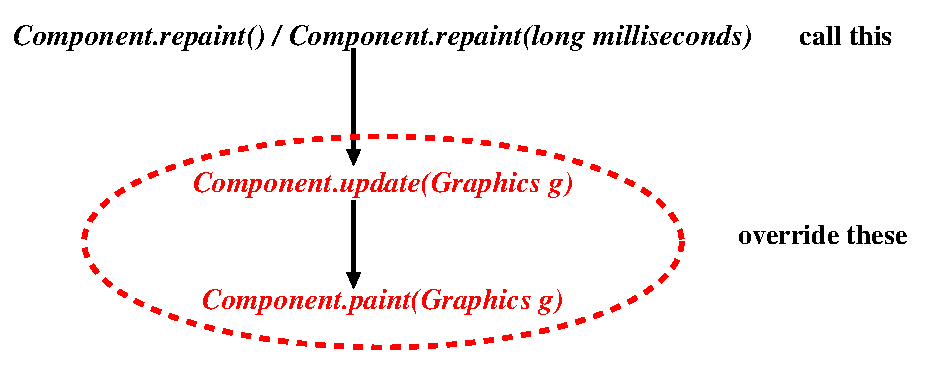
\includegraphics[width=\textwidth]{Figures/PaintMethod.eps}
    \caption{The default behaviour of the painting methods of components in the AWT package.}
    \label{fig:PaintMethod}
  \end{center}
\end{figure}

Having learned the basic graphical tools of the AWT with the help of
the most easy plot program, we can now apply what we have just learned
to the simulation of the radioactive decay.
\inputlisting{Listings_Java/RadioactiveDecay_easyplot.java}
Implementing the graphical facilities in the
\verb|RadioactiveDecay.java| code is easy. The output of 
the new program can be seen in figure \ref{fig:RDEasyPlot}.
\begin{figure}[htbp]
  \begin{center}
    \includegraphics[angle=-90,width=\textwidth]{Figures/RadioactiveDecayEasy.eps}
    \caption{The output of the easyplot version of the radioactive 
      decay program.}
    \label{fig:RDEasyPlot}
  \end{center}
\end{figure}

In the program code we immediately recognize
in the lines  56 to 81 the \verb|paint()| method. The results of the
simulation have to be scaled appropriately to fit in the Frame. The
curve is plotted with the method \verb|drawLine()|. Since we want to
plot also the exact analytical solution for the mean values in red we
set
\begin{verbatim}
  g.setcolor(Color.red)
\end{verbatim}
in line 74 before drawing the corresponding curve.

It is important to note that in the lines 21 to 24 
we have added the code
\begin{verbatim}
  frame.addWindowListener(...);
\end{verbatim}
which allows to handle the request to close the window. These ``events''
are in the \verb|java.awt.event| package and will be discussed later
in chapter \ref{sec:AWTAdvanced}. 

\subsection{Ptplot -- Extending Javas Graphics Capabilities}
The quality of the plot of the simulation results are rather poor
compared to high standards we are used to today. It is clear, that we
could now go on refining the plot with the help of the Java
AWT. Although this might be an interesting and instructive task, it is
not our primary interest in this book. Fortunately, there are advanced
2D graphics components which can be used in applets and
applications. One of these packages is Ptplot (you pronounce it
pee--tee--plot). The Ptplot package is released under the liberal UC
Berkley copyright. It has been developed by Edward A. Lee, C. Hylands,
and W. Wu. You are free to download it at
\href{http://ptolemy.eecs.berkeley.edu/java/ptolemy.plot2.0/ptolemy/plot}%
         {http://ptolemy.eecs.berkeley.edu/java/ptolemy.plot2.0/ptolemy/plot}
where you also find
the documentation and many demos of Ptplot. 

The components of Ptplot have the following properties:
\begin{itemize}
\item plots are embeddable in applets and applications
\item you may use binary or ASCII data
\item the plots are auto--ranging
\item you may label automatically or manually the axes
\item logarithmic axes
\item live, animated plots
\item infinite zooming
\item  various plot styles (connected lines, scatter plots, bars, ..)
\item various point styles (none, dots, points, ....)
\item multiple data sets and legends
\item color or black and white plots
\item error bars.
\end{itemize}
Before writing the first program using Ptplot take a look at the
class hierarchy of Ptplot in figure \ref{fig:PtplotHierarchy}.
\begin{figure}[htbp]
  \begin{center}
    \leavevmode
    \setlength{\unitlength}{.8cm}
    \input{Figures/PtplotHierarchy1.pic}\\[.3cm]
    \input{Figures/PtplotHierarchy2.pic}
    \caption{The class hierarchy of the Ptplot package.}
    \label{fig:PtplotHierarchy}
  \end{center}
\end{figure}

Let us now look at a very simple program in order to demonstrate
what you need to invoke the Ptplot methods.
\inputlisting{Listings_Java/Ptplot_Demo1.java}

We see that we have to import additionally the  Ptplot package. The
class \verb|ptplot_Demo| extends the class \verb|PlotApplet|. Again we
want to run the code as applet as well as an application so the class
does have a main method. In lines 14 to 17 we instantiate the new Frame
and activate the WindowListener as we did it in the
\verb|RadioactiveDecay_ploteasy.java| code. The actual plot routines
are in lines 28 to 33. In the \verb|init()| method we invoke the method
\verb|super.newPlot()| to create a new plot, \verb|super.init()| to
initialize it and \verb|plot().setTitle| to give the plot a title.

A second possibility of using Ptplot, which we prefer to use, is to extend
the \verb|Applet| class instead of the \verb|PlotApplet| class and 
change the lines 28 to 33 to:
\lstinputlisting[first=28,last=33]{Listings_Java/Ptplot_Demo2.java}
The difference is that the \verb|PlotApplet| class realizes a kind
of interface for an applet to start plot commands confirming to the
pxgraph commands and executes them from parameters given in the applet.
Pxgraph is a program for the X windows system to plot data using
batch files like gnuplot. The full pxgraph functionality is
included in the ptplot package and can be used. For further documentation
concerning this point, please refer to the ptplot documentation.

Next we want to draw the results of the simulation of the radioactive
decay process with the help of Ptplot and learn at the same time how
to exploit the features of Ptplot. The corresponding code can be seen
below.
\inputlisting{Listings_Java/RadioactiveDecay_ptplot.java}
The output of the code can be seen in Fig. (\ref{fig:ptplotOutput}). 
\begin{figure}[htbp]
  \begin{center}
    \leavevmode
    \includegraphics[angle=-90,width=\textwidth]{Figures/RadioactiveDecay_ptplot.eps}
    \caption{The output of the RadioactiveDecay\_ptplot.java program.}
    \label{fig:ptplotOutput}
  \end{center}
\end{figure}

The actual plotting code starts in line 55 and ends in line 79. 
There we use several methods of the \verb|ptplot.Plot|
class and of the superclass \verb|PlotBox| of the \verb|Plot| class.
All methods are called \verb|setMethod| where \verb|Method| is
self-explaining. Several other methods are implemented in the
\verb|Ptplot.PlotBox| class and its child, the \verb|Ptplot.Plot| class. 
They are summarized in table \ref{tab:PtplotMethods}. 
\begin{table}[htbp]
  \begin{center}
    \small
    \leavevmode
    \begin{tabular}{p{5cm}|p{8cm}}
      Method & Purpose \\\hline\hline
      \verb|addLegend(int, String)| & draw a legend for one plot number\\
      \verb|addXTick()| & \\
      \verb|addYTick()| & \\
      \verb|setBackground(Color)| & set the background color of plot\\
      \verb|setForeground(Color)| & set the foreground color of plot\\
      \verb|setGrid(boolean)| & draw a grid \\
      \verb|setLabelFont(String)| & font for axis labels and legend labels  \\
      \verb|setTitle(String)| & title of graph \\
      \verb|setTitleFont(String)| & set title font \\
      \verb|setXLabel(String)| & label of x axis \\
      \verb|setYLabel(String)| & label of y axis \\
      \verb|setXLog(boolean)| & x axis logarithmic scaling \\
      \verb|setYLog(boolean)| & y axis logarithmic scaling \\
      \verb|setXRange(double, double)| & x range of the plot \\
      \verb|setYRange(double, double)| & y range of the plot \\\hline
      \verb|addPoint(int, double, double, boolean)| & add a point to the plot,
      the boolean var. decides, if the point gets connected with the last one.
      The integer var. is the plot number.\\
      \verb|addPointWithErrorBars(int,| 
                     \verb|double, double, double, double, boolean)| & %
      add a point to the plot with errorbars. Th additional vars. specify the
      lower and higer y coordinate of the error bar.\\
      \verb|setBars(boolean)| & bar plotting on or off \\
      \verb|setBars(double, double)| & define width and offset for bar 
      plotting and enable bar plotting. \\
      \verb|setImpulses(boolean)| & plot impulses \\
      \verb|setMarksStyle(String)| & none, points or various \\
    \end{tabular}
    \caption{Overview of all the Ptplot methods in the Plot and PlotBox classes.}
    \label{tab:PtplotMethods}
  \end{center}
\end{table}

Although this is the most common way of using ptplot in this book, there
is another feature coming with ptplot. It can read data files and plot
the data. For this you have to write a script, which contains the
commands for the plot to be created. This scripting language
is borrowed from the \emph{pxgraph} program. It is like using ``gnuplot''
 with
its scripting facilities. For details you can look at the 
documentation coming with the ptplot package. For us it will be
easier to read the files into Java and then use ptplot to plot it on 
screen.

%%%%%%%%%%%%%%%%%%%%%%%%
\subsection{3D plots in Java -- Java3D}
Sometimes you are forced to use 3D plots to visualize your data
and therefore it is natural to ask for a package to accomplish
three dimensional plots. Unfortunately to our knowledge there is
(yet) no freely available package in Java for 3D plots. Ptplot
can only handle 2D plots and JSci can handle only some very
basic 3D plots (see chapter \ref{sec:JSci}).

There is also a program called 
\verb|SciVis|\footnote{\href{http://kopernik.npac.syr.edu:8888/scivis/}%
  {http://kopernik.npac.syr.edu:8888/scivis/}},
which is completely written in Java and allows for 2D and 3D plots
in many different ways. But up to now, there are only C and
Fortran interfaces to supply data to it. You can also read from
files, but first you have to understand the data format, which is
described in the users guide.
The authors told us they are developing a Java interface to
supply data directly to \verb|SciVis|. 

At the moment, the best solution is to write the data to a file
and use an external program available to you. The most common
denominator would possibly be ``gnuplot'', which is available for many
different platforms and can create a lot of different 3D plots.

Since Java 2, there is a new (external) API -- not included in the JDK 1.2
disribution, you have to get it seperatly -- called \emph{Java3D}. 
This is a full implementation of three dimensional routines to
produce all kinds of 3D scenes and objects and even move these scenes.
With this API it seems to be possible to write a fairly easy
3D plotting program in the near future. So this lack of features
in Java for the scientist should be gone soon. 

%%%%%%%%%%%%%%%%%%%%%%%%%%%%%
\subsection{Using (system dependent) external programs like gnuplot}
There is a last way of obtaining 3D plots ``in Java'': You can use
an external program like Gnuplot or any other command line tool and
call it from a Java program. This of course is not system independent
and is not recommended unless you are desperatly needing it.

In Java there is a class called \verb|Runtime| in the \verb|java.lang|
package, which consists of all kind of methods to change and
use the environement you are running your Java program in. This can be used
to start a subprocess of the running Java program. So starting an
external process from a Java program can be done in two steps:
\begin{itemize}
\item Get a \verb|Runtime| object of the running Java program.
\item Start a new process as a subprocess of the given \verb|Runtime| object.
  You have to use the \verb|exec(String)| instance method of the  \verb|Process|
  class for this. 
\end{itemize}
You can also read the standard output of the subprocess and use it in your 
Java program. To demonstarte how it actually works, we give two examples:
\begin{enumerate}
\item A Java program starts a Gnuplot program, which plots a sine curve.
  \inputlisting{Listings_Java/Gnuplot.java}
\item A Java program executes a ``ls -al'' command on a UNIX machine,
  which just gives the directory listing. For a Windows system you just
  use the ``dir'' command instead.
  \inputlisting{Listings_Java/DirectoryListing.java}
  This time we also wait for the execution of the process to finish and 
  then read the standard output and display it on the screen.
\end{enumerate}

%%%%%%%%%%%%%%%%%%%%%%%%%%%%
\subsection{Printing in Java and with Ptplot}
Now that we have learned how to make plots in Java, it is of great
importance to get a printed version of our graphics. For
this purpose Java has commands for initiating a print job and preparing
the output for the printer. Java always produces potscript output.
Because the procedure has changed
from Java 1.1 to Java 2, we only present the Java 1.1 version not
to confuse you. In Java 1.0 there have been no methods for 
printing in  Java, you would have to use screen capture programs
for example.

Because printing is of course system dependent, it is not as easy
as issuing a print command, but it is still managable. 
In Java printing is done basically in four steps:
\begin{enumerate}
\item Get a \verb|Toolkit| for the component you want to print. 
  Use method \verb|getToolkit()| in the \verb|java.awt.Component| class.
\item Get a \verb|PrintJob|. Use the 
  \verb|getPrintJob(Frame f, String printjobname, Properties printprops)|
  method in the \verb|java.awt.Toolkit| class.
\item Start ``printing'':
  \begin{enumerate}
  \item Get the graphics context for the component in question. Use the
    \verb|getGraphics()| method of the \verb|java.awt.PrintJob| class.
  \item Print the desired part of the component. If you want to print 
    everything contained by the component use the \verb|printAll()|
    method, otherwise use just the \verb|print()| method of the
    \verb|Component| class.
  \item Send the data to the printer or file by using the \verb|dispose()|
    method of the \verb|java.awt.Graphics| class.
  \end{enumerate}
\item Finish printing and close dialog box. Use \verb|end()| method of
  the \verb|java.awt.PrintJob| class.
\end{enumerate}
The program \verb|RadioactiveDecay_printing.java| demonstartes the use of
the printing capabilities of Java. 
\lstinputlisting[first=32,last=47]{Listings_Java/RadioactiveDecay_printing.java} 

Of course there are some drawbacks to talk about. First of all with
this code you always get the output in a size referring to your actual
picture on the screen, it does not use the full paper size. If you want
to use the whole page size available you have to scale the component
to be plotted to the full size and scale back after printing. This is
what we do in the convenience class we have written for easy printing
in the simulation package. 

So if you want to print a component scaled to the full size, you use
the \verb|PrintComponent.Dialog()| method in the simulation package.
It scales your component to the full size -- no matter if it should be
on a portrait or landscape page -- and sends the scaled picture to the
printer or a postscript file. After printing it scales back to the
size it had before. The whole code above could therefore be
substituted by the line
\begin{verbatim}
  import simulation.*;
  ....
  PrintComponent.Dialog(frame, plot, "Radioactive Decay");
\end{verbatim}
Because most of the time you need postscript (or EPS) files of the
created plots or graphics, this is the most common use of the
printing features for a scientist.

A second method of the \verb|simulation| class called \verb|DialogNoScaling()|
can be used to produce unscaled output of the component or container.
I thas the same syntax as the \verb|Dialog()| method before.

There is one caveat to mention: if you are going to insert the
produced postscript files into TeX/LaTeX, you will have to do
some editing on the postscript files. First of all you have to
add a bounding box line at the beginning of the postscript
file. You can do this by hand, put a line (for a portrait figure)
\begin{verbatim}
 %%BoundingBox:  0 0 595 840
\end{verbatim}
at the beginning of the postscript file (You can adapt the numbers
to the figure at hand and check the area by viewing it in 
ghostscript/ghostview.) or you can use a program to automatically
calculate and insert a bounding box command (like e.g. epstool,
gsview on Windows, etc.). The second change is to remove all the 
lines between \verb|%%BeginSetup| and \verb|%%EndSetup| except
a possible rotate line like \verb|90 rotate 0 -595 translate|.
This is necessary, because some strange effects appear in the
resulting \verb|.dvi| or \verb|.ps| file after "texing".

Another drawback might be the resolution of the postscript file.
This happens especially when printing GUI components and is not
present when plotting ptplot plots fortunately. Java kind of rasters
the screen display and because the screen resolution is much worse 
than the printer resolution this gives unpleasant results. It also
gives strange results if you scale a large GUI to a small A4 or Letter
format for printing, which could look very ugly or even miss some
of the displayed objects. But as already mentioned, most of the time
we only need plots in postscript files and this works great with
the code above.

In Java 2 there has been some small changes to the printing
interface. A new class has been introduced in Java2: \verb|java.awt.print|.
This class provides much more sophisticated methods and it is even
able of handling color models, which is very important for
color handling and printing. This is a big step ahead, but for the
details we refer to the API documentation, because it is also a
bit more difficult to understand.

Ptplot 2.1 printing facilities ????? (EPS)

\paragraph{Printing from an Applet}
Usually applets are not allowed to initiate printjobs, unless
a \verb|SecurityManager|, another important Java class, explicitly
allows for it. Most of the time the browser or appletviewer has
to initiate the printjob, allowed by the security manager. You can of
course always use the printing facilities of the browser and plot
the whole panel visible in the browser.


What you can do is, write a main method in the applet and start
it as an application. Do the plots  and print them from the
application. 

If you use a security manager and are allowed to print, you need a
frame for your applet, because the  \verb|getPrintJob()| command
only takes a frame and not an applet as first argument. So just
put a frame into the applet and then put the applet inside the frame.


%%%%%%%%%%%%%%%%%%%%%%%
\subsection{The Results of the Simulation}

The results of the simulation are plotted in Fig. (\ref{FIG_DECAYA}) and 
(\ref{FIG_DECAYB}).
\begin{figure}
\label{FIG_DECAYA}
\begin{center}
\includegraphics[angle=-90,width=8cm]{Figures/RadioactiveDecay_1.eps}\\
\includegraphics[angle=-90,width=8cm]{Figures/RadioactiveDecay_2.eps}
\end{center}
\caption{Two realizations of the stochastic process of the radioactive decay.
The first one with linear y axis scaling and the second one uses a logarithmic
y axis scaling. The blue lines are the exact solution and the red ones
are the simulations.
The parameters of the simulation were choosen to be $N_0 = 100; 
\quad p = \lambda \Delta t = 0.01 s^{-1}; \quad \Delta t = 1\text{s};
\quad t_{\text{end}} = 300\text{s}$}
\end{figure}
\begin{figure}
\label{FIG_DECAYB}
\begin{center}
\includegraphics[angle=-90,width=11cm,clip]{Figures/RadioactiveDecay_3.eps}\\
\end{center}
\caption{The same as figure \ref{FIG_DECAYA}, but with different parameters:
$N_0 = 1000; \quad p = \lambda \Delta t = 0.03 s^{-1}; 
\quad \Delta t = 1\text{s};  \quad t_{\text{end}} = 100\text{s}$}
\end{figure}
 It is 
immediately recognized that the simulation results fluctuate around 
the expected curve. This is of course not astonishing since the 
exact result holds for mean values. In order to achieve a better
agreement with the decay law it is necessary to run the simulation
several times and to take the average over the different 
realizations of the decay process. This can easily be achieved by 
a simple modification of the program \verb|RadioactiveDecay_ptplot.java|.
 We introduce an additional input variable, the number of realizations
\verb|nreal| and accordingly implement a loop over the different 
realizations. This can be best seen in the listing of the 
new program \verb|RadioactiveDecay_ptplot2.java|.
\lstinputlisting[first=61,last=63]%
          {Listings_Java/RadioactiveDecay_ptplot2.java}

At the end of the realizations loop
we have to perform the average. This is seen in lines 61 to 63.
(STRESS MORE THE IDEA OF REALIZATIONS!!!!; allgemeine Strategie erlaeutern.)

Note that in order to speed up the program we have modified slightly 
the algorithm  so that we can save a loop. ?????
The probability to observe one decay in time $\Delta t$ is
\begin{equation}
p = \beta \Delta t
\end{equation}
where $\beta = \lambda N$ and $\Delta t$ must be small enough so 
that $\beta \delta t \ll 1$. 
From the elementary rules of combinatorics we know that
the probability to observe $n$ decays in time $t=m\Delta t$ is therefore
given by
\begin{equation}
P = p^n(1-p)^{m-n} {m \choose n}.
\end{equation}
Inserting the definition of $p$ the above expression can be cast 
in the form
\begin{equation}
P = \left( \frac{\beta t}{m}\right)^n 
     \left( \frac{1 - \beta t}{m} \right)^{m-n}
      \frac{m!}{(m-n)! n!}.
\end{equation}
Performing the limit $\Delta t \longrightarrow 0$ (i.e. $m 
\longrightarrow \infty$) and considering that
\begin{equation}
\left(1-  \frac{\beta t}{m} \right)^{m} \longrightarrow 
            \exp(-\beta t),
\end{equation}
\begin{equation}
\left( 1- \frac{ \beta t}{m} \right)^{-n} \longrightarrow 
            1,
\end{equation}
and
\begin{equation}
\frac{m!}{(m-n)! n!} \longrightarrow m^n
\end{equation}
we obtain the result
\begin{equation}
P = \frac{\mu^n \exp(-\mu)}{n!},
\end{equation}
where $\mu = \beta t$. The above distribution is the well know
Poisson distribution.

\subsubsection{Plot Methods in the Simulation Package}
Because sometimes it is easier to use ready made routines, we
have added some plotting convenience classes and methods to
get the plots faster. If you take the shortcut presented here
or you want to use the low level ptplot interface does not 
matter, it is totally up to you.

?????
\paragraph{plot2D()}
\paragraph{errorBars()}
\paragraph{histogram()}
\paragraph{barPlots()}

It is now easy to verify that the number of decays in a given 
interval is distributed according to the Poisson distribution.
To this end we have counted the number of decays in a given 
interval. This is accomplished in the lines xy. At the end of the
program we plot in a histogram the distribution of the number of 
decays and overlay the expected Poisson
distribution.  

\subsubsection{Listing of the full Program}
\lstinputlisting{Listings_Java/RadioactiveDecay_ptplot2.java}


Run the program for the following two sets of parameters:
\begin{eqnarray*}
N_0= 100, p = 0.001 s^{-1}, \Delta t = 1s, t = 100s \\
N_0= 100, p = 0.0001 s^{-1}, \Delta t = 1s, t = 100s
\end{eqnarray*}
with nreal = 100 and nreal = 1000.

The result of  two simulations can be seen in figs. x and y.
\begin{figure}
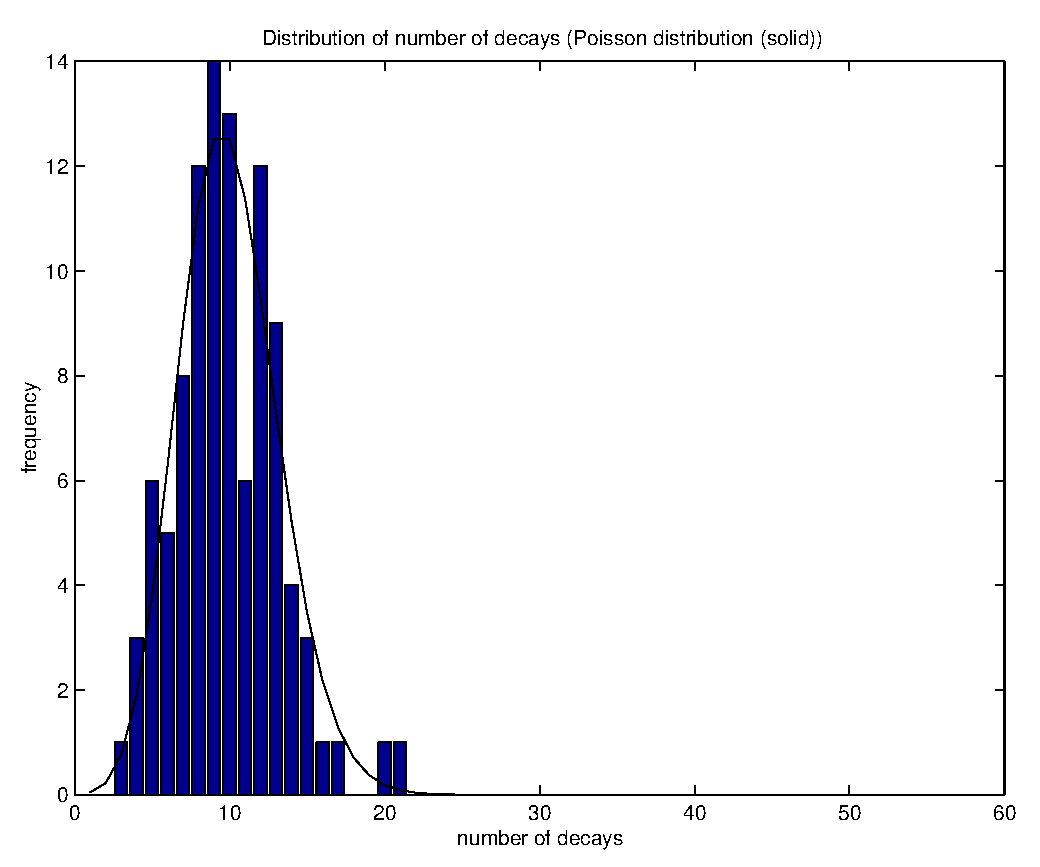
\includegraphics[width=\textwidth]{Figures/f_decay1.eps}
\caption{The distribution of the number of decays computed with 
the program decayr. 100 realizations. The simulation was run for
N0=100 and lambda=0.001.}
\end{figure}

\begin{figure}
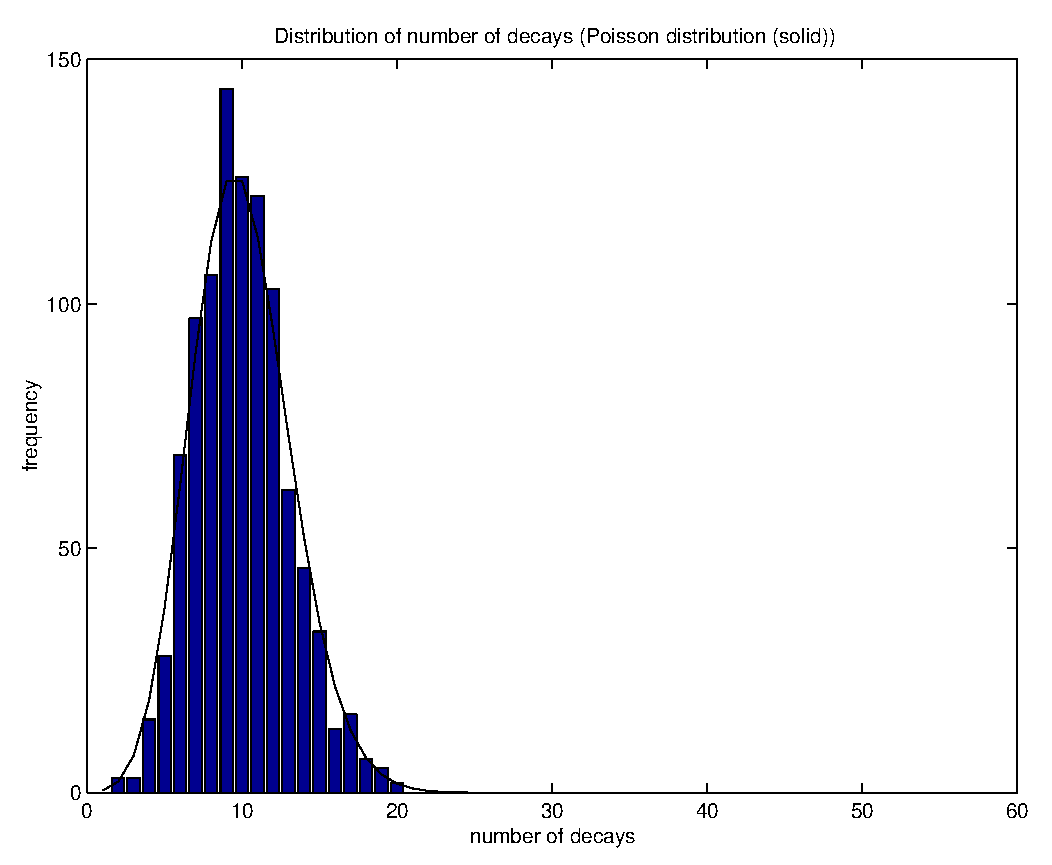
\includegraphics[width=\textwidth]{Figures/f_decay2.eps}
\caption{The distribution of the number of decays computed with 
the program decayr. 1000 realizations. The simulation was run
for N0=100 and lambda = 0.001.}
\end{figure}

%%%%%%%%%%%%%%%%%%%%%%%%%%%%%%%%%%%%%%%%%%%%%%%%%%%%%%%%%%%%%%%%%%%%%%
\section{Simple Monte Carlo Evaluation of Integrals}
It is the purpose of this subsection to introduce Monte Carlo Methods
in the context of the numerical evaluation of definite integrals.
We will see in later chapters that Monte Carlo integration is the
method of choice when treating multidimensional
integrals numerically. As a typical rule of thumb
``classical'' deterministic methods are outperformed
by Monte Carlo methods  for systems with a large number of 
degrees of freedom.
For simplicity and to stress the basic ideas 
it is convenient at the moment to consider one--dimensional definite
integrals of the form
\begin{equation}
\label{INTEGRAL}
I = \int_a^b dx f(x).
\end{equation}
Obviously such integrals can be evaluated analytically for many
integrands
$f(x)$.  However, there are as well many cases for which a numerical
evaluation is necessary.

Before introducing the Monte Carlo approach to numerical integration
let us remind the basic ``classical'' deterministic approach to
numerical integration. The standard approach is based upon the
geometrical interpretation of the integral (\ref{INTEGRAL}) as the
area under the curve of the function $f(x)$ between the points $a$ and
$b$. In the simplest algorithm this area (see figure) is approximated
as a sum over rectangles. To this end the $x$--axis is divided into
$n$ equally spaced intervals of width $\Delta x$,
\begin{equation}
\Delta x = \frac{b-a}{n}
\end{equation}
whose ends are given by
\begin{equation}
x_i = x_0 + i\Delta x
\end{equation}
for $i=1, \ldots ,n$. Of course, $x_0 = a$ and $x_n =b$. Thus in the
so--called rectangular approximation the integral is evaluated as
\begin{equation}
\label{I_CLASSICAL}
I_n = \Delta x \sum_{i=0}^{n-1} f(x_i).
\end{equation}
Of course, other more accurate approximations are possible.

How can we now evaluate the above integral by drawing random numbers?
The standard way is based on a very simple idea. 
From the introductory course in analysis we know that the Mean 
Value Theorem states that the exact value of the integral $I$ is 
given by
\begin{equation}
I= (b-a) f(\zeta)
\end{equation}
for some value of $\zeta$ in the interval $a \le \zeta \le b$. $f(\zeta)$
represents the average value of the function $f(x)$ 
in the interval $[a,b]$. Thus we could also write
\begin{equation}
I = (b-a) \langle f \rangle,
\end{equation}
where $\langle  \rangle$ denotes the mean value.
Let us draw $n$
random numbers which are uniformly distributed in the interval $[a,b]$
and let us sample the corresponding value of $f(x_i)=f_i$. The Monte Carlo
estimate $I_n$ of the integral $I$ is then the sample mean, which is
given by
\begin{equation}
\label{MCI_STANDARD}
I_n = \frac{(b-a)}{n} \sum_{i=1}^{n} f(x_i),
\end{equation}
where $n$ is the number of trials. Amazingly the form of the above
estimate is very similar to the classical formula (\ref{I_CLASSICAL}).
The fundamental difference is that now the $n$ points at which the
function $f$ is evaluated are no longer equally spaced but randomly 
distributed.

There is also the possibility to compute the integral $I$
stochastically
with the help of the ``Hit or Miss'' algorithm. The idea behind
this algorithm is again very simple. To be explicit we imagine a rectangle
of height $h$ and width $(b-a)$ such that the function $f(x)$ lies
within the rectangle (see figure; Gould, p.329). To evaluate the
integral we draw randomly pairs of uniformly distributed random
numbers $(x_i,y_i)$ such that $a \le x_i \le b$ and $0 \le y_i \le h$.
In other words the probability to draw a point within the rectangle is
given by the inverse of the area $A$ of the rectangle,
i.e. $1/(b-a)h$. It is now evident how the area under the
function $f$ may be estimated. The fraction of points $(x_i,y_i)$
which satisfy the condition $y_i \le f(x_i)$ is an estimate of the
ratio of the integral $I$ to the area $A$ of the rectangle. Hence,
drawing $n$ random pairs the estimate $I_n$ of $I$ by this ``scoring''
method is given by
\begin{equation}
I_n = A \frac{n_s}{n},
\end{equation}
where $n_s$ is the number of ``hits'', i.e., of points lying below the
curve $f(x)$.

Before writing two simple programs to elucidate the above algorithms
it is important to have in mind that both estimates are affected by
statistical errors. Let us consider for simplicity 
the standard method. Since the $f(x_i)$ are random we know 
from the elementary theory of data analysis
that an appropriate measure of the error is given by the variance
which is defined by
\begin{equation}
{\rm Var}(f) = \langle f^2 \rangle - \langle f \rangle^2.
= \langle (f -\langle f \rangle)^2 \rangle
\end{equation}
Since we draw a finite number of random numbers we can
estimate the mean value by using
\begin{equation}
\hat{f}  = \frac{1}{n} \sum_{i=1}^n f(x_i) 
\end{equation}
and correspondingly the estimate of the variance by using
\begin{equation}
{\rm Var}(f(x_1),\ldots, f(x_n)) = \frac{1}{n-1} \sum_{i=1}^n 
   (f(x_i)- \hat{f})^2 = \sigma_f^2.
\end{equation}
The quantity $\sigma_f = \sqrt{{\rm Var}(f_1, \ldots, f_n)}$ 
is also called the standard deviation. In the previous expression
we have used the short--hand
notation $f(x_i) = f_i$. However,
we are not interested in the error of $f$ but in the error of the
estimate $I_n$, which is a sum over random numbers. 

Repeating the 
simulation and hence drawing other random numbers we will get another
estimate of $I_n$. Therefore, repeating the simulation $m$ times 
we can estimate the mean of $I_n$ as
\begin{equation}
\hat{I_n} = \frac{1}{m} \sum_j^m I_n(j)
\end{equation}
and the corresponding variance as
\begin{equation}
{\rm Var}(I_n(1), \ldots, I_n(m)) = 
\frac{1}{m-1} \sum_j^m (I_n(j) - \hat{I_n})^2 = \sigma_I^2
\end{equation}
We will denote the above variance also by $\sigma_I^2$.
Of course, proceeding this way is not very practical since we
have to perform the simulation $m$ times. A much more economical
estimation of the error of the mean of $I_n$ could be achieved by 
establishing a simple relation between $\sigma_I$ and the standard 
deviation of the individual trials $\sigma_f$. To this end we 
introduce the discrepancy $\delta f_i$ between the
individual trial $f_i$ and its mean $\langle f \rangle$. The 
discrepancy $\delta I_n$ between $I_n$ and its mean value can be
obtained to first order in the $\delta f_i$ by a simple Taylor 
expansion (error propagation rules)
\begin{equation}
\delta I_n = \sum_{i=1}^n \frac{\partial I_n}{\partial f_i} \delta 
f_i.
\end{equation}
Hence, it follows from the above equation by taking the average over
$\delta I_n^2$ that
\begin{equation}
\langle \delta I_n^2 \rangle = \sum_{i,j=1}^{n}
    \frac{\partial^2 I_n}{\partial f_i \partial f_j} 
     \langle \delta f_i \delta f_j \rangle.
\end{equation}
It is plausible to assume, that 
$\langle \delta f_i \rangle = 0$
for all $i$ and that the $\delta f_i$ are not correlated
for $i \neq j$, i.e.,
$\langle \delta f_i \delta f_j \rangle = \langle f_i \rangle \langle f_j \rangle$
and that for $i=j$ we have $\langle \delta f_i^2 \rangle = \sigma_f$ 
for all $i$ it follows from the above equation that
\begin{equation}
\sigma_I^2 = \sum_{i=1}^n \left(
      \frac{\partial I_n}{\partial f_i} \right)^2 \sigma_f^2
      = \frac{1}{n^2} n \sigma_f^2 = \frac{\sigma_f^2}{n}
\end{equation}
and finally we have the useful relation
\begin{equation}
\sigma_I = \frac{\sigma_f}{\sqrt{n}}.
\end{equation}
The mean error of the mean scale with 1 over the square root of 
the number of individual trials. The precision of the estimate 
thus increases only slowly with the number of trials (remark: central
limit theorem: see Chapter 2).

Now we are in the position to write two programs to implement the above
stochastic algorithms. In order to be specific we compute the integral
\begin{equation}
I = \int_0^1 dx \sqrt{1-x^2} = \frac{\pi}{4}.
\end{equation}
In other words we want to estimate the number $\pi$ by Monte Carlo
methods.

We begin by the standard method. The listing of an according 
program can be seen below.

\subsubsection{Listing of the program mcpi.}
\inputlisting{./Listings/mcpi.m}

We run the program for $n=10, 100, 1000, 10000$. The result of the 
four simulations can be seen in Fig. xy.
\begin{figure}
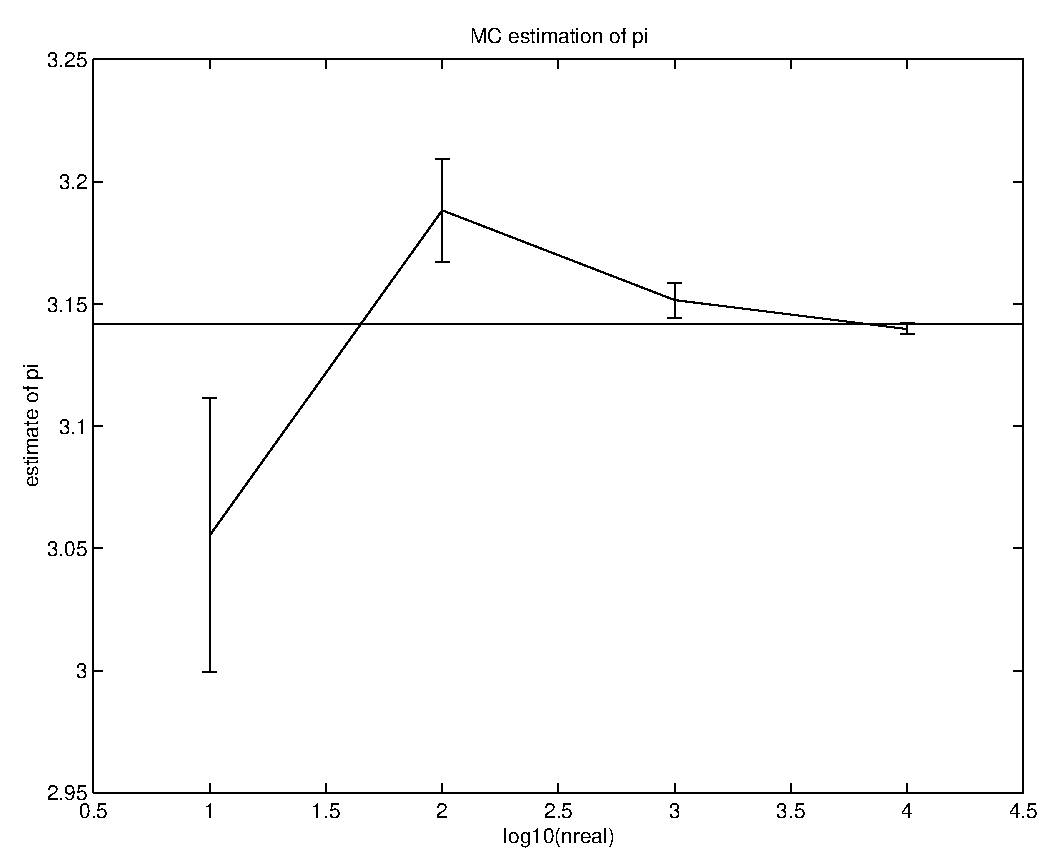
\includegraphics[width=\textwidth]{Figures/plotmcpi.eps}
\caption{The estimation of pi for n=10,100,1000,10000. The 
error bars correspond to the standard deviation of the mean of the 
estimate.}
\end{figure}

Next we write a program for the scoring  method. 

\subsubsection{Listing of the program mcpiscore.m}
\inputlisting{./Listings/mcpiscore.m}

Again we run the simulation for n=10, 100, 1000, 10000.
The result of a simulation can be seen in the next Figure.
\begin{figure}
\begin{center}
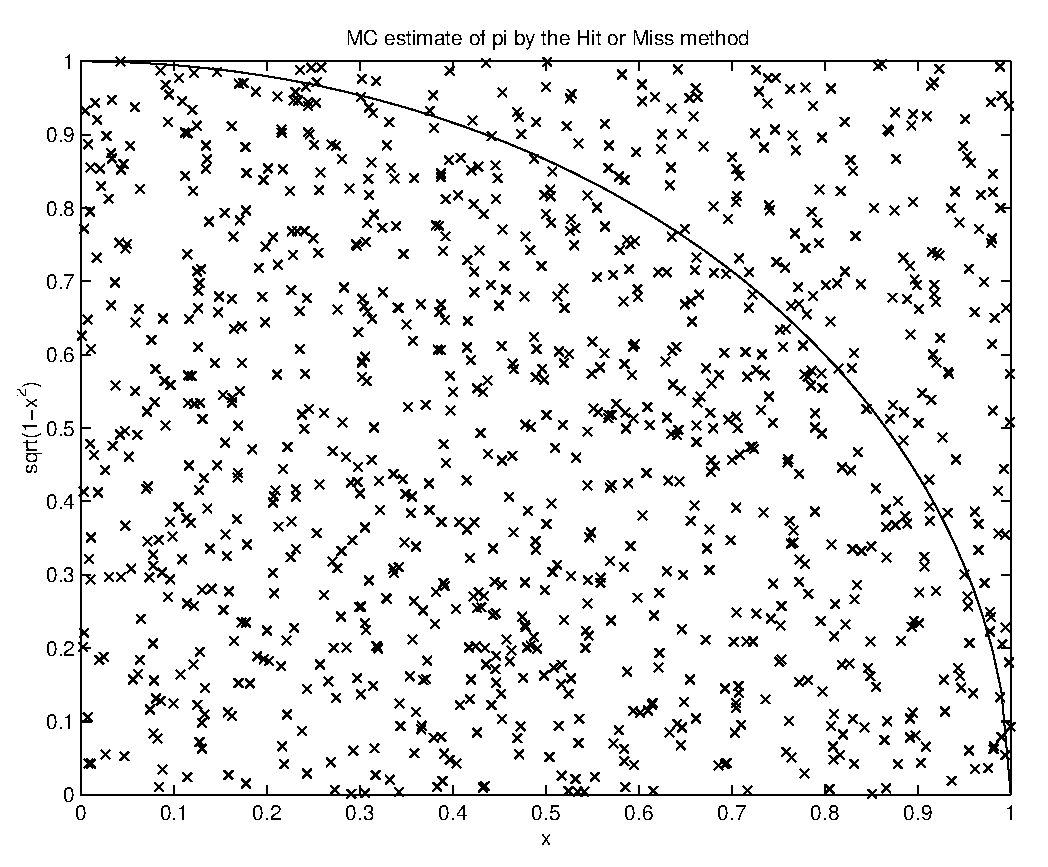
\includegraphics[width=.7\textwidth]{Figures/fmcpiscore.eps}
\end{center}
\caption{The scoring method. The continuous line represents
the function $\sqrt{(1-x^2)}$.}
\end{figure}


%%%%%%%%%%%%%%%%%%%%%%%%%%%%%%%%%%%%%%%%%%%%%%%%%%%%%%%%%%%%%%%%
\section{Beyond this chapter}


%%%%%%%%%%%%%%%%%%%%%%%%%%%%%%%%%%%%%%%%%%%%%%%%%%%%%%%%%%%%%%%%
\section{Exercises}

Use the  Matlab function \texttt{rand()}
to solve the following problems (don��t care about the quality and
the algorithm of the random number generator, for now):

\begin{Ex}
\label{Photoabsorption}
\textbf{Photoabsorption \cite[]{reif:67}} \\
Consider the absorption of photons passing through a gas in two dimensions.
We model the gas by introducing slabs of width $dx$ and density $n$ (in
particles per area), which absorb the incident photons. The slab
particles have a cross-sectional area of $\sigma$.

So the probability of a photon to be absorbed in the slab will be
($M$ is the number of particles in the slab of the height $dy$)
$$ P(\text{Photon absorbed}) = \frac{M\sigma}{dy} =
      \frac{\sigma n dx dy}{dy} = \sigma n dx  \quad .$$
We have assumed that there is no overlap between the cross-sections of
the slab particles.

Write a program to simulate this process on the computer. Take $N$
incident photons and watch the number of particles left over
against the slabs passed in a diagram. Do this simulation several
times and calculate the ensemble-average. What process you know
is similar to this behaviour and what takes the place of the spatial
dimension in that case?

%If we now have N identical slabs in a row, the probability of passing
%through all the slabs would be $(1-p)^N$, if the transmissions
%are statistically independent of each other.
%Then for a slab of finite thickness $X=N dx$ with $N\to\infty$, we
%get the Transmission probability
%$$ P(\text{transmitted through $N$ slabs}) =
%       \left(1-\frac{n\sigmaX}{N}\right)^N \quad .$$

%Now simulate the following systems:
%identical photons are absorbed in one slab ($N$ slabs)
\end{Ex}

\begin{Ex}
\label{Monte-Carlo_Integration}
\textbf{Monte-Carlo Integration -- Speed and Accuracy} \\
Write a program for the calculation of the following integral:
$$ \int_0^1 \frac{1}{1+x^2} dx\quad .$$
\begin{enumerate}
\item using the hit and miss method
\item using the standard method
\end{enumerate}
For both algorithms, calculate the mean and the standard deviation
as discussed in the lecture. Also use the analytical result of the
integral to calculate $\pi$. Compare the accuracy of both algorithms
using the approximations of $\pi$. Compare the speed of the two
programs by using the \texttt{cputime} function in Matlab.
(e.g. type the following to time the random number generator:
\texttt{t=cputime;x=rand(1000);cputime-t})

To that end, create a table and a plot with the two parameters
($n$: the number of intervals and $N$: the number of realizations)
against
the accuracy (use at least 5 values). To save time, you can first
check for a good $n$  and then do the plots only against $N$.
For the speed, plot the cputime against the achieved accuracy for
many different $N$.
\end{Ex}

\begin{Ex}
\label{Euler_Constant}
\textbf{Euler��s Constant using Monte-Carlo Algorithm %
          \cite[]{mohazzabi:98}} \\
Suppose throwing $N$ darts randomly at a dart board, which has been
divided into $R$ equal size regions. The probability of hitting one region
is $p=1/R$. Then the probability of hitting an empty region
(not already occupied by a dart) is $(1-p)^N$. Using the binomial
distribution, you can get the probability for hitting a region with
$m$ darts. If you choose
the number of regions equal to the number of darts
thrown on the board, we have $p=1/N$ and therefore
$$ P(\text{hitting an empty region}) = \left( 1-\frac{1}{N} \right)^N\quad .$$

Because the above series converges to $e$ for $N\to\infty$, we can use
the following method to get an approximation of the Euler constant:
\begin{enumerate}
\item[(i)] Throw randomly a large number of darts (say $N$) on a board, which has
  been divided into $N$ equal size regions.
\item[(ii)] Count the number of empty regions (call it $N_0$).
\item[(iii)] The fraction $N/N_0$ is a good estimate of the Euler constant $e$.
\end{enumerate}

Write a program for that algorithm and check the results. You can even
use $N/N_1$, if $N_1$ is the number of regions with the occupancy of
one dart. Check this, too. What $N$ do you need to
get the same accuracy using the formula? And how many terms of the
series for $e$ ($\sum_{i=0}^\infty 1/i! = e$)?
\end{Ex}

%%%%%%%%%%%%%%%%%%%%%%%%%%%%%%%


\bibliographystyle{peter}
\bibliography{V_98,simulit}

%%% Local Variables: 
%%% mode: latex
%%% TeX-master: "V_98"
%%% End: 


%%%\lstset{language=matlab}

%%% Chapter 2 
%%%%%%
%%%%%% Chapter 2
%%%%%%

\chapter{Stochastic Variables}
Since the notion of random variables will be essential
for the understanding of stochastic methods this chapter will be 
devoted to the introduction of the fundamental concepts of 
probability theory.

%%%%%%%%%%%%%%%%%%%%%%%%%%%%%%%%%%%%%%%%%%%%%%%%%%%%%%%%%%%%%%%%%%
\section{The Nature of Probabilities}
In the previous chapter we have already made use of probabilistic 
notions in an intuitive way. However, we have not asked the 
following question: What are probabilities? How can we formulate 
the notion of probability in such a way that it is useful for 
physical applications?

Essentially, there are three possible definitions of probability
\cite{BRODY}:
a) the axiomatic interpretation, b) the frequency interpretation, and
c) the ensemble interpretation.


\subsection{The Axiomatic Interpretation}
The axiomatic definition \cite{FELLER} of probabilities has been proposed by 
Kolmogorov in 1933. The formal objects to which we want to 
attribute probabilities are called {\em events} and are subsets
of a basic set $\Omega$ which is called the {\em event space} or in 
physical applications the {\em phase space}. If the event $e$ 
belongs to $\Omega$, so does its complement $\Omega - e$ also; the 
null event $\oslash$ is therefore also in $\Omega$. Events 
containing only one member of $\Omega$ are called the elementary events
of $\Omega$.

A function $P(e)$, called the {\em probability} of $e$ can be 
assigned to each event $e$ in $\Omega$. The function $P(e)$ has
the following properties:

(i) $P(e) \ge 0$ for all $e$ in $\Omega$;

(ii) $P(\Omega) = 1$;

(iii) If $e_1, e_2, \ldots $ are in $\Omega$ and are pairwise
disjoint, i.e., $e_i \cap e_j = \oslash$ when $i \ne j$, then
$P(e_1 \cup e_2 \cup \ldots ) = P(e_1)+P(e_2) + \ldots$.

It follows immediately from the above three axioms that

(iv) If $\bar{e}$ is the complement of $e$, i.e., the set of all 
events which are not in $e$, then
$P(\bar{e}) = 1- P(e)$;

(v) $P(\oslash) = 0$.



\subsection{The Relative Frequency Interpretation}
In his attempt to axiomatize probability theory, von Mises
introduced in 1919 the notion of a {\em Kollektiv}, which stands
for a single infinite sequence of random events such as the 
outcomes of throwing a coin. He defined then the probability of some 
event to be the limit of its relative frequency in such a series of 
observations when the series becomes infinitely long (the 
Kollektiv) \cite{COMPAGNER,BRODY}. 
If we denote by $n$ the number of data in the series,
by $m(e)$ the number of times the event is observed in it, then
the probability $P(e)$ is defined as
\begin{equation}
P(e) = \lim_{n \rightarrow \infty} \frac{m(e)}{n}.
\end{equation}
Of course, such a series of events must have the property that any 
infinite subsequence in it must have the same limit. 

The problem with this definition is the following one: How can any 
sequence of experimental data, which will be always be finite, 
have the properties of such a Kollektiv? In practice the 
relative frequencies for subsequencies will always differ from 
that in the main sequence.

To illustrate the problems with the frequency interpretation of
probabilities we consider the following example. We throw a die 
$n$ times and
look at the relative frequency $m(4)$ of the outcome of throwing a 
4. This experiment will be simulated with the help of the 
following program.

{\bf Listing of the program relfreq.}
\inputlisting{./Listings/relfreq.m}

The result of an experiment for up to 400 throws is shown in Fig. 
(\ref{F_FRELFREQ}). Running the program again we observe 
another approach to the asymptotic
value. We recognize immediately the difficulties with von Mises 
definition of probability.
\begin{figure}
\label{F_FRELFREQ}
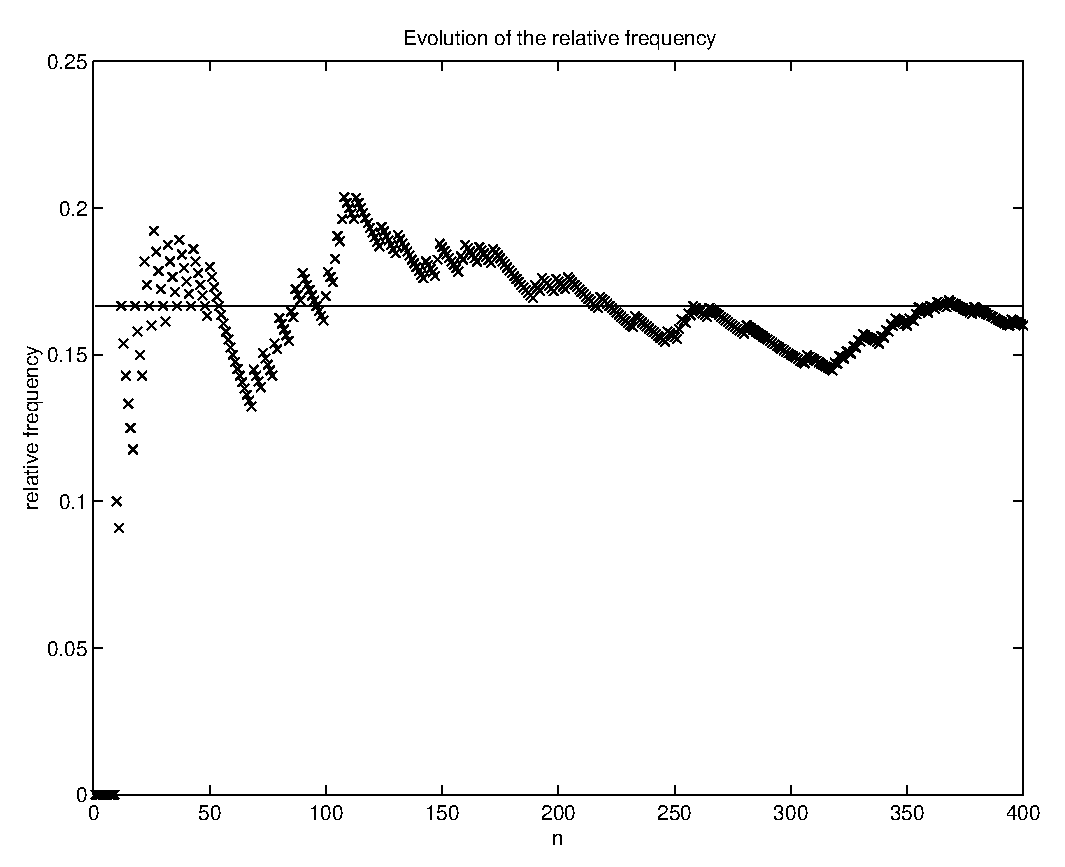
\includegraphics[width=10cm]{frelfreq.eps}
\caption{Simulation of the evolution of the relative frequency of throwing
a 4 in play of die.}
\end{figure}

\subsection{The Ensemble Interpretation}
We know from statistical mechanics  the notion of {\em ensemble}. An
ensemble is a collection of a large number $N$ of equally prepared
systems (equal models). A simple example is the microcanonical
ensemble, 
which is the
ensemble of all microstates in phase space, which are characterized by
fixing the macroscopic values for the the energy $E$, the volume $V$
and the number of particles $N$.

The abstract concept of an ensemble allows naturally the definition
of a mean value. We have to consider two cases:

(i) The ensemble contains a finite, discrete number of models: 
Let $n$ be the number of models and $Q(i)$ the interesting quantity in
model $i$. The ensemble mean value $\langle Q \rangle$ is then defined
as
\begin{equation}
\langle Q \rangle = \sum_{i=1}^n \frac{Q(i)}{n}.
\end{equation}

(ii) The models are characterized by some continuous parameter, i.e.,
the initial positions of molecules in a gas: If we name the continuous
parameter $\omega$, the phase space as $\Omega$ , and $n(w)$ a weight
function characterizing the ensemble, then
\begin{equation}
\langle Q \rangle = \frac{ \int_{\Omega} Q(\omega) dn(\omega)}
                         {\int_{\Omega} dn(\omega)}.
\end{equation}
Usually, the function $n(\omega)$ can be derived on the basis of the
theoretical model on which the ensemble relies upon. 

Let us consider as a simple example from equilibrium statistical 
mechanics a gas consisting of $N$ particles. The microstates of 
the system are the points $(q,p) = (\vec{r}_1, \vec{r}_2, \ldots, \vec{r}_N,
\vec{p}_1,\ldots, \vec{p}_N)$ in the 6--dimensional phase space.
The probability to find the microsystem at time $t_0$ in a volume 
element $dV=d^{3N}qd^{3N}p$ around $(q,p)$ is given by
\begin{equation}
dw(q,p) = \rho(q,p) d^{3N}qd^{3N}p,
\end{equation}
where $\rho(q,p)$ is the distribution function. For the 
microcanonical ensemble  the distribution function $\rho$ simply 
reads
\begin{equation}
\rho(q,p) = \left\{ 
\begin{array}{ll}
c= {\rm const}, &{\rm for} \quad E-\Delta \le H(q,p) \le E, \\
0, &{\rm otherwise}
\end{array} \right.
\end{equation}

Probabilities can be introduced as a special kind of ensemble 
average. Let $A$ be a property, which 
the members of the ensemble may have or not and let us define an indicator
function
\begin{equation}
\chi_A(\omega) = \left\{ 
\begin{array}{ll}
1, & {\rm if \quad member \quad labelled} \quad \omega {\rm \quad has 
\quad property\quad} A \\
0, & {rm if not}.
\end{array}\right.
\end{equation}
The probability of $A$ in the ensemble is  simply defined as 
the ensemble average of $\chi_A(\omega)$
\begin{equation}
P(A) = \langle \chi_A(\omega) \rangle = 
\frac{\int_{\Omega} \chi_A(\omega) dn(\omega)}{\int_{\Omega} 
dn(\omega)}.
\end{equation}
The probability is the relative weight in the ensemble of those 
members that have the property $A$. In the case of a discrete 
ensemble the above definition of probability reduces to a sum over
the members of the ensemble having the property $A$
\begin{equation}
P(A) = \sum_{i=1}^{n} \frac{\chi(i)}{n},
\end{equation}
i.e., the probability is the relative frequency of the members 
having the property $A$ in the ensemble.

It is clear that from the above definition of probability its is
possible to derive the Kolmogorov axioms of probability theory.

It is important to stress that the
ensemble is a purely theoretical construction and has to be adapted 
to the physical situation of interest as we will see in the future chapters. 
Furthermore, it is to be noted that the ensemble 
interpretation  allows the definition of time dependent 
probabilities,
i.e.,
\begin{equation}
P(A,t) = \langle \chi_A(t) \rangle,
\end{equation}
which are of fundamental importance while studying stochastic 
processes.

%%%%%%%%%%%%%%%%%%%%%%%%%%%%%%%%%%%%%%%%%%%%%%%%%%%%%%%%%%%%%%%%%%
\section{The Definition of Stochastic Variables}
A stochastic variable $X$ is an object which is defined by a space 
of states (space of events, phase space) and by a probability 
density over this set. The space of state may be discrete, e.g. 
the numbers 1,2,3,4,5,6 for a play of dice or the number of 
molecules in a chemical reaction, as well as continuous, e.g.
the velocity of a Brownian particle. Of course, the space of state
may also be discrete and continuous at the same time, e.g., the
energy of an electron in the presence of some binding centers.
When sampling a one dimensional continuous stochastic variable $X$,
the probability to find some value in the infinitesimal interval
$(x,x+dx)$ will be expressed symbolically by
\begin{equation}\label{DENSITYDEF}
P(x) dx \equiv {\rm Prob} \{X\in [x,x+dx] \},
\end{equation}
which defines the probability density $P(x)$ associated with the 
stochastic variable $X$. It follows immediately from the above 
equation and from the addition law of
probability theory that the probability to sample a value of $X$
in the interval $[a,b]$ is given by
\begin{equation}\label{DENSITYDEF2}
\int_a^b dx P(x) = {\rm Prob}\{ X \in[a,b] \}.
\end{equation}
It is evident from Eqs. (\ref{DENSITYDEF}) and (\ref{DENSITYDEF2}) that 
the probaility density is non--negative, i.e. $P(x) \ge 0$ and 
that it is normalized
\begin{equation}
\int_{-\infty}^{\infty} dx P(x) = 1.
\end{equation}
For later convenience we remark that the probability density may 
contain also sums over $\delta$--functions. For example $P(x)$ can 
also have the form 
\begin{equation}
P(x) = \sum_n p_n \delta(x-x_n) + \tilde{P}(x),
\end{equation}
where
$\tilde{P}(x) \ge 0$, $p_n \ge 0$, $\tilde{P}$ integrable  
and the normalization condition is
\begin{equation}
\sum_n p_n + \int dx \tilde{P}(x) =1.
\end{equation}

The distribution function $F$ of the stochastic variable $X$ is 
defined by 
\begin{equation}
F(x) \equiv {\rm Prob}\{X \le x\}.
\end{equation}
The density function and the distribution function are related by 
the equation
\begin{equation}
F(x) = \int_{-\infty}^x dx' P(x'),
\end{equation}
or equivalently by $F'(x)= P(x)$.

\subsection{Further Characterization of Stochastic Variables}
A stochastic variable is completely defined by the space of states 
and by the probability density function. However, it is helpful to 
introduce some other quantities in order to characterize them.

The {\em expectation value}, i.e. the average,  of any function $f(X)$ 
with respect to the stochastic variable $X$ is denoted by
$\langle f(X) \rangle$ and is defined by
\begin{equation}
\langle f(X) \rangle = \int dx f(x) P(x).
\end{equation}
Of particular importance are the {\em moments} of a distribution. The 
$m$--th moment $\mu_m$ is defined as $\langle X^m \rangle$. Of 
course, $\mu_1$ is the {\em mean}. The variance ${\rm Var}(X)$ 
is defined as
\begin{equation}
{\rm Var}(X) \equiv \langle (X - \langle X \rangle )^2\rangle
   = \mu_2 - \mu_1^2,
\end{equation}
and is the square of the standard deviation $\sigma$.

Another important quantity is the {\em characteristic function} $G(k)$. It is 
defined as
\begin{equation}
G(k) = \langle \exp(ikx) \rangle = \int_I \exp(ikx) P(x) dx,
\end{equation}
and has the obvious properties
\begin{equation}
G(0) = 1 \quad {\rm and} \quad |G(k)| \le 1.
\end{equation}
The characteristic function is also called the {\em the moment 
generating function}, because expanding the exponential function 
in a Taylor series we get 
\begin{equation}
G(k) = \sum_{n=0}^{\infty} \frac{i^n}{n!} k^n 
      \langle X^n \rangle.
\end{equation}
Thus, if $G(k)$ is known the moments are easily evaluated as
\begin{equation}
\left. \frac{d^n}{dk^n}G(k) \right| = i^n \langle X^n \rangle.
\end{equation}
The same function serves to generate the so--called cumulants
which are defined as
\begin{equation}
\ln G(k) = \sum_{n=1}^{\infty} \frac{(ik)^n}{n!} \kappa_n,
\end{equation}
and are combinations of the moments, i.e., the first three 
cumulants are given by
\begin{eqnarray}
\kappa_1 &=& \mu_1, \\
\kappa_2 &=& \mu_2 - \mu_1^2 =\sigma^2, \\
\kappa_3 & = & \mu_3 - 3 \mu_2 \mu_1 + 2 \mu_1^3.
\end{eqnarray}
It can be shown \cite{Gardiner} that the cumulant generating 
function  cannot be a polynomial of degree greater than 2, that 
is, either all but the first two cumulants vanish or there is an 
infinite number of nonvanishing cumulants.

REMARK ( kappai given then g(k) unique !!!???????????�) 

\subsection{Some Important Random Variables}
Let us first introduce and discuss briefly some important 
continuous one dimensional probability densities.

\subsubsection{The Uniform Density}
The simplest density is the uniform density which is constant if $x$
lies within the interval $[a,b]$ and zero otherwise, i.e.,
\begin{equation}
P(x) = 1/(b-a).
\end{equation}
It is easy to check that the mean of the uniform distribution is
\begin{equation}
\langle X \rangle = \frac{a+b}{2}
\end{equation}
and that the standard deviation of a uniformly distributed random variable 
is
\begin{equation}
\sigma = \frac{b-a}{2\sqrt{3}}.
\end{equation}
As we will see the uniform probability density will play a 
fundamental role in the forthcoming chapters.

\subsubsection{The Exponential Density Function} 
The exponential density function is defined as
\begin{equation}
P(x) = a \exp(-ax),
\end{equation}
where $a$ is any positive constant. It is easy to verify that
the mean and the standard deviation of an exponentially distributed random 
variable are equal
\begin{equation}
\langle X \rangle = \sigma = \frac{1}{a}.
\end{equation}

\subsubsection{The Gaussian or Normal Density Function}
The most important density function for physics is the 
gaussian probability density. It has the form
\begin{equation}
P(x) = (2\pi a^2)^{-1/2} \exp[-(x-x_0)^2/2a^2],
\end{equation}
for $a$ positive and $-\infty < x_0 < \infty$.
The mean and the standard deviation of the Gaussian probability 
density are given by $\mu_1 = x_0$ and by $\sigma =a$, 
respectively. The characteristic function of the Gaussian density reads
\begin{equation}
G(k) = \exp(i \mu_1k - \frac{1}{2} \sigma^2 k^2),
\end{equation} 
which means that $\kappa_1 = \mu_1$, $\kappa_2 = \sigma^2$ and 
that all higher cumulants vanish.

\subsubsection{The Cauchy or Lorentz Density} 
The Cauchy or Lorentz density is defined as
\begin{equation}
P(x) = \frac{1}{\pi} \frac{a}{(x-x_0)^2 + a^2}
\end{equation}
for positive $a$ and $-\infty <x_0 < \infty$. It is an example of 
a probability density which does not have a finite variance. In 
fact, not even the integral defining  the mean value converges. 

Let us now discuss some typical discrete probability densities.
The discrete random variable will be denoted by $N$.

\subsubsection{The Discrete Uniform Probability Density} 
The discrete uniform probability density is defined by
\begin{equation}
P(n) = \frac{1}{n_2 -n_1 +1}
\end{equation}
for $n_1 \le n \le n_2$ and zero otherwise. Of course,
$n_1$ and $n_2$ are integer numbers and $n_1 \le n_2$.
Its mean value is
\begin{equation}
\langle N \rangle = \sum_n n P(n) = \frac{n_1 +n_2}{2} 
\end{equation}
and its variance
\begin{equation}
\sigma^2 = \frac{(n_2 -n_1)(n_2 -n_1+2)}{12}.
\end{equation}
The above equations are easily proven with the help of the 
relations
\begin{equation}
\sum_{n=1}^N n= \frac{N(N+1)}{2}; \sum_{n=1}^{N} n^2 = \frac{N(N+1)(2N+1)}{6}. 
\end{equation}

\subsubsection{The Binomial Distribution}
Let us assume that the random variable $Y$ 
can take only two values $\{y_1,y_2\}$, the probability for the 
value $y_1$ being $p$ and correspondingly for $y_2$ (1-p). If we 
consider $N$ realizations of the stochastic variable $Y$ the 
probability to find the value $y_1$ $N$ times under the $n$ results
is the binomial density $P(n)$
\begin{equation}
P(n) = \frac{N!}{n!(N-n)!} p^n(1-p)^{(N-n)},
\end{equation}
for $0 \le n \le N$.
The mean and variance of the binomial density are given by
\begin{equation}
\langle n \rangle = Np,
\end{equation}
and
\begin{equation}
\sigma^2 = Np(1-p).
\end{equation}
It is easy to check the normalization of the binomial distribution since
\begin{equation}
1 = [p + (1-p)]^n = \sum_{n=0}^N \frac{N!}{n! (N-n)!}
        p^n (1-p)^{(N-n)}.
\end{equation}

\subsubsection{The Poisson Density}
The Poisson density as we already know
is defined as
\begin{equation}
P(n) = \frac{\exp(-a) a^n}{n!},
\end{equation}
for $n > 0$ and $a \in R$. The mean value and the variance
of the Poisson density are equal,
\begin{equation}
\langle n \rangle = \sigma^2 = a.
\end{equation}
As we already know from the discussion of the radioactive decay the 
Poisson density is a limit of the 
binomial probability density for $N \rightarrow \infty$, $p \rightarrow 
0$ while $Np=a={\rm const}$. Another limit of the Poisson density
which deserves consideration is the limit $a \gg 1$: In this limit
the Poisson density will be essentially different from zero only 
for $n \approx a$. For $n \gg 1$  the Stirling formula 
holds
\begin{equation}
n! \approx (2 \pi n)^{1/2} n^n \exp(-n)
\end{equation}
so we can write
\begin{equation}
\ln\left[ \frac{\exp(-a) a^n}{n!} (2\pi a)^{1/2} \right] 
\approx (n-a) -n\ln\left(\frac{n}{a}\right).
\end{equation}
Setting $\epsilon=(n-a)/2$ and since, 
for $\epsilon \ll 1$ $\ln(1+\epsilon) \approx \epsilon -
\epsilon^2/2$ and for $n\approx a$
we can write
\begin{equation}
\ln\left[ \frac{\exp(-a) a^n}{n!} (2\pi a)^{1/2} \right] \approx
-(n-a)^2\frac{1}{2a}.
\end{equation}
So that finally for $a \gg 1$
\begin{equation}
\frac{\exp(-a) a^n}{n!} \approx \exp\left( - 
\frac{(n-a)^2}{2a}\right).
\end{equation}
Thus, in the limit $a \gg 1$ the Poisson density resembles a
Gaussian density with mean $a$ and variance $a$.

\subsection{Multivariate Random Variables}
Up to now we have considered only one dimensional stochastic 
variables. Obviously, $n$ random variables $X_1, X_2, \ldots, X_n$ 
which are sampled simultaneously can be interpreted as the 
components of an $n$--dimensional stochastic variable $X$.
Their joint density function
$P_n(x_1, \ldots, x_n)$ is defined through the statement
\begin{equation}
P_n(x_1, \ldots, x_n)dx_1 dx_2 \ldots dx_n \equiv
{\rm Prob}\{ X_i \in (x_i,x_i+dx_i) \quad \text{for 
each} \quad i=1, \ldots , n\}.
\end{equation}
If we look at the subset of stochastic variables $X_1, \ldots 
X_s$, for $s>n$ we can easily write down with the help of the
elementary laws of probability theory the joint density function for 
this set irrespective of $X_{s+1}, \ldots, X_n$
\begin{equation}
P_s(x_1, \ldots, x_s) = \int P_n(x_1, \ldots, x_s, x_{s+1}, \ldots 
x_n) dx_{s+1} \ldots dx_{n}.
\end{equation}
$P_s$ is a so--called {\em marginal distribution}.

The {\em conditional density} 
$P_{s|n-s}(x_1,\dots,x_s|x_{s+1},\ldots,x_n)$ is the joint 
density of $X_1, \ldots , X_s$
given that $X_{s+1}=x_{s+1}$, \ldots , $X_n = x_n$ and is easily 
shown to be given by Bayes rule
\begin{equation}
P_{s|n-s}(x_1,\dots,x_s|x_{s+1},\ldots,x_n) =
\frac{P_n(x_1, \ldots, x_n)}{P_{n-s}(x_{s+1}, \ldots, x_n)}.
\end{equation}

Two subsets $(X_1, \ldots, X_s)$ and $(X_{s+1}, \ldots, X_n)$ are 
said to be statistically  independent if $P_n$ factorizes
\begin{equation}
P_n(x_1, \ldots, x_n)=P_s(x_1, \ldots, x_s)P_{n-s}(x_{s+1}, \ldots, 
x_n).
\end{equation}
In this case $P_s$ is the marginal as well as the conditional 
probability density.

The definition of moments is easily generalized to the  
multivariate case
\begin{equation}
\langle X_1^{m_1} \ldots X_n^{m_n} \rangle =
\int x_1^{m_1} \ldots x_n^{m_n} P(x_1, \ldots, x_n) dx_1 \ldots 
dx_n.
\end{equation}
Accordingly, the characteristic function is given by
\begin{equation}
G(k_1, \dots, k_n) = \left\langle 
\exp[i(k_1X_1 + \ldots +k_n X_n)]\right\rangle.
\end{equation}
Again the multivariate Taylor expansion in the variables $k_i$ 
generates the moments
\begin{equation}
G(k_1, \dots, k_n) = \sum \frac{(ik_1)^{m_1} \ldots (ik_n)^{m_n}}
                  {m_1! \ldots m_n!} 
       \langle X_1^{m_1} \ldots X_n^{m_n} \rangle.
\end{equation}
For completness we mention that the cumulants 
$\kappa(X_1^{m_1} \ldots X_n^{m_n})$ are defined as
\begin{equation}
\log G(k_1, \dots, k_n) = {\sum}' \frac{(ik_1)^{m_1} \ldots (ik_n)^{m_n}}
                  {m_1! \ldots m_n!} 
       \kappa(X_1^{m_1} \ldots X_n^{m_n}),
\end{equation}
where the symbol $\sum'$ idicates that we do not have to sum when 
all $m$ vanish. As an example we give the $n \times n$ covariance
matrix $\kappa(X_i X_j)$
\begin{eqnarray}
{\rm Cov}(X_i, X_j) &=& 
 \langle (X_i-\langle X_i \rangle)(X_j-\langle X_j \rangle)\rangle 
 \\
 & = & \langle X_i X_j \rangle - \langle X_i \rangle \langle X_j 
           \rangle.
 \end{eqnarray}
The diagonal elements of the covariance matrix are, of course, the 
variances, whereas the off--diagonal elements are called the 
covariances.
With the help of the covariance matrix it is possible to define a 
correlation coefficient
\begin{equation}
\rho_{ij} = \frac{\kappa(X_i X_j)}{\sqrt{\kappa(X_i^2) 
\kappa(X_j^2)}}.
\end{equation}
For $n=2$ the statistical independence of $X_1$ and $X_2$ can be 
expressed through one of the following criteria: 

(i) All moments 
factorize, i.e., $\langle X_1^{m_1} X_2^{m_2}\rangle= 
\langle X_1^{m_1}\rangle \langle X_2^{m_2}\rangle$. 

(ii) The 
characteristic function factorizes, i.e., $G(k_1,k_2) = 
G(k_1)G(k_2)$. 

(iii) All cumulants $\kappa(X_1^{m_1}X_2^{m_2})$ 
vanish when both $m_1$ and $m_2$ differ from zero. Two variables $X_1$
and $X_2$ are called uncorrelated if their covariance is zero. 
This condition is weaker than statistical independence.

A typical example of a multivariate density is the density of the multivariate 
Gaussian distribution
\begin{equation}
\label{MULTI_GAUSS}
p(\vec{x}) = \frac{(2\pi)^{-n/2}}{(\det A)^{1/2}}
     \exp\left( -\frac{1}{2} (\vec{x} - \vec{\mu})_i (A^{-1})_{ij} 
     (\vec{x}-\vec{\mu})_j \right),
\end{equation}
where $A$ is a symmetric, positive definite matrix with elements 
$A_{ij}$. It is straightforward to check that the mean value of $\vec{X}$
is given by
\begin{equation}
\langle \vec{X} \rangle = \vec{\mu},
\end{equation}
that the covariance matrix is given by
\begin{equation}
{\rm Cov}(X_i, X_j) = A_{ij},
\end{equation}
and that the generating function is
\begin{equation}
G(\vec{k}) = \exp(-\frac{1}{2} k_i A_{ij} k_j + i \mu_ik_i).
\end{equation}

%%%%%%%%%%%%%%%%%%%%%%%%%%%%%%%%%%%%%%%%%%%%%%%%%%%%%%%%%%%%%%%%%%
\section{The Random Variables Transformation Theorem}
We will discuss in this subsection a very helpful theorem by 
Gillespie. The proof of the theorem can be found in the book by
Gillespie \cite{GILLESPIE} or in his paper \cite{GILLESPIE_THEOREM}. 

We know already that a stochastic variable is defined by 
specifying its space of states and its probability density.
Here, we consider the $n$--dimensional random variables $X=(X_1, \ldots, X_n)$ 
which are specified by their joint probability density function
$P(x_1, \ldots, x_n)$. Let $f_i$ be functions of the $n$ variables. With the 
help of the $f_i$ we map the $n$ random variables $X_1, \ldots, X_n$ 
onto $m$  new random variables $Y_1, \ldots, Y_m$ by
\begin{equation}
Y_i = f_i(X).
\end{equation}
The random variable transformation theorem now states that the 
probability density of the new stochastic variable $Y$ is given by
the expression
\begin{eqnarray}
\label{RVT}
P(Y_1, \ldots, Y_m) &=& \int dx_1 \ldots dx_n \prod_{i=1}^{m} 
\delta(y_i - f_i(x_1, \ldots, x_n)) P(x_1, \ldots, x_n).
\end{eqnarray}
The integrals extend over the range of all $X_i$.
For a proof of the random variable transformation theory see 
Gillespie.

\subsection{The Addition of Stochastic Variables}
As a first simple example of the application of the random 
variable theorem we consider the addition of two stochastic 
variables $X_1$ and $X_2$ with joint probability density
$P(x_1,x_2)$. The probability density $P(Y) $ of a new stochastic variable
$Y$ which is defined as the sum of $X_1$ and $X_2$ 
\begin{equation}
Y = X_1 + X_2
\end{equation}
is then given by
\begin{equation}
P(y) = \int \int \delta(x_1 +x_2 -y) P(x_1,x_2) dx_1 dx_2.
\end{equation}
We can perform the integration over $x_1$ to obtain
\begin{equation}
P(y) = \int P(x_1,y-x_1) dx_1.
\end{equation}

For the special case of two statistically independent random 
variables $X_1$ and $X_2$ the above equation simplifies to the 
following expression
\begin{equation}
P(y) = \int P_{X_1}(x_1)P_{X_2}(y-x_1) dx_1.
\end{equation}

It is now easy to check that the following equations hold
for the mean value and for the variance of the new stochastic 
variable $Y=X_1 + X_2$
\begin{equation}
\mu(X_1 +X_2) = \mu(X_1) + \mu(X_2)
\end{equation}
and
\begin{equation*}
{\rm Var}(X_1 + X_2) = {\rm Var}(X_1) + {\rm Var}(X_2) +
            2 {\rm Cov}(X_1,X_2).
\end{equation*}
The last equation implies that only for uncorrelated stochastic 
variables we have the simple relation 
${\rm Var}(X_1 + X_2) = {\rm Var}(X_1) + {\rm Var}(X_2)$.

The above results for the mean values and variances can easily be 
generalized to the so called linear combination theorem. For any
set of random variables $X_1, \ldots, X_n$ and any set of 
constants $a_1,\ldots, a_n$ we have
\begin{equation*}
\mu\left\{  \sum_{i=1}^n a_i X_i \right\} =
     \sum_{i=1}^n a_i \mu(X_i) 
\end{equation*}
and
\begin{equation*}
{\rm Var}\left\{  \sum_{i=1}^n a_i X_i \right\} = 
    \sum_{i=1}^n a_i^2 {\rm Var}(X_i) + 
    2 \sum_{i=1}^{n-1} \sum_{j=i+1}^n a_i a_j {\rm Cov}(X_i,X_j).
\end{equation*}



\subsection{One--to--One Transformations}
Let us consider the following application of the random variables
transformation theorem. Let $X$ be a random variable with
probability density $P(x)$ and let the random variable $Y$ be 
defined as $Y=f(X)$. Then the density function of $Y$ is given by
\begin{equation}\label{ONE_TO_ONE}
P(y) = \int_{-\infty}^{\infty} dx P(x) \delta(y-f(x)).
\end{equation}
For the case that the function $f$ is a smooth, one--to--one
transformation the equation $y=f(x)$ can be solved uniquely for $x$
as $x=f^{-1}(y)$. Let us now change the integration variable in 
Eq. (\ref{ONE_TO_ONE}) from $x$ to $z=f(x)$
\begin{equation*}
P(y) = \int_{-\infty}^{\infty} dz \left| {f^{-1}}'(z) \right|
      P(f^{-1}(z)) \delta(y-z),
\end{equation*}
where we have made use of
\begin{equation*}
dx = \left|{f^{-1}}'(z) \right| dz.
\end{equation*}
Integrating over $z$ yields
\begin{equation*}
P(y) = P(f^{-1}(y)) \left|{f^{-1}}'(y) \right|.
\end{equation*}
Since $x=f^{-1}(y)$, then $|dx/dy|=|{f^{-1}}'(y))|$, and we can 
rewrite the above equation as
\begin{equation*}
P(y) = P(x) \left|  \frac{dx}{dy} \right|
\end{equation*}
which is a very important formula in the theory of stochastic 
variables which we will use, e.g., in the next chapter.

The previous result is easily generalized to many dimensions.
If the transformations $Y_i =f_i(X_1, \ldots, X_n)$ for $i=1,\ldots,n$ are 
one--to--one, then the probability density of the variables $Y_i$ 
is given by
\begin{equation*}
P(y_1, \ldots, y_n) = P(x_1, \ldots, x_n) 
     \left|  \frac{\partial(x_1, \ldots, x_n)}
     {\partial(y_1, \ldots, y_n)} \right|.
\end{equation*}

BEMERKUNG: ANALOGIE ZUR ANALYSIS !!!!!!!

\subsection{The Central Limit Theorem}
As an essential application of the random variable transformation 
theorem we prove the central limit theorem.
Let us consider $N$ statistically independent random variables $X_i$
with the same probability density $P$, and, of course, the same mean $\mu$
and the same variance $\sigma^2$. With the help of the $X_i$ we 
define a new random variable $Z_n$ as
\begin{equation}
Z_N \equiv \frac{1}{\sqrt{N}} \sum_{j=1}^N (X_j - \mu).
\end{equation}
Since the $X_i$ are assumed to be mutually statistically 
independent their joint probability density is
$P(x_1) \cdots P(x_N)$. By the random variable transformation 
theorem the probability density of $Z_N$ is given by
\begin{equation}\label{PZN}
P(z_N) = \int dx_1 \ldots dx_N \prod_{i=1}^N P(x_i) 
    \delta\left(z_N -\frac{1}{\sqrt{N}} \sum_{j=1}^N (X_j -\mu) 
    \right).
\end{equation}
Using the integral representation of the $\delta$--function
\begin{equation}
\delta(x-x_0) = \frac{1}{2\pi} \int ds \exp[is(x-x_0)]
\end{equation}
the $\delta$--function in Eq. (\ref{PZN}) can be written as
\begin{eqnarray}
&&\delta\left(z_N -\frac{1}{\sqrt{N}} \sum_{j=1}^N (X_j -\mu) 
    \right) \\
&=& \frac{1}{2\pi} \int_{-\infty}^{\infty} ds \exp(isz_N) \prod_{j=1}^N 
    \exp[-isN^{-1/2}(x_j - \mu)].
\end{eqnarray}
Inserting the above equation into Eq. (\ref{PZN}) and changing the 
order of the $x$ and $s$ integrations we obtain
\begin{eqnarray}
P(z_N) &=& \frac{1}{2 \pi} \int ds \exp(isz_N) \nonumber \\
    & & \times \prod_{j=1}^N \int dx_j P(x_j) 
        \exp[-isN^{-1/2}(x_j - \mu)].
\end{eqnarray}
The above expression can be written more concisely in the form
\begin{equation}\label{PZMITG}
P(z_N) = \frac{1}{2\pi} \int ds \exp(isz_N) 
[G(\frac{s}{\sqrt{N}})]^N,
\end{equation}
where we have introduced the characteristic function $G$ by
\begin{equation}
G(\chi) \equiv \int dx P(x) \exp[-i\chi(x-\mu)].
\end{equation}
The function $G$ can be expanded in a Taylor series
\begin{equation}\label{TAYLORG}
G(\chi) = G(0) + \chi G'(0) + \frac{\chi^2}{2} G''(0) + O(\chi^3).
\end{equation}
Since the $n$--th derivative of $G$ is given by
\begin{equation}
G^{(n)}(\chi) = 
    \int_{-\infty}^{\infty} dx P(x) [-i(x-\mu)]^n \exp[-i\chi(x-\mu)].
\end{equation}
For $\chi=0$ the above expression evidently reduces to
\begin{equation}
G^{(n)}(0) = (-i)^n \langle (X-\mu)^n\rangle.
\end{equation}
In particular we find $G(0) =1$, $G'(0)= 0$ and $G''(0) = 
-\sigma^2$.
Therefore, Eq. (\ref{TAYLORG}) can simply be written as
\begin{equation}
G(\chi) = 1 - \frac{\sigma^2\chi^2}{2} + O(\chi^3).
\end{equation}
Inserting the above equation into Eq. (\ref{PZMITG}) 
and putting $\chi=s/{\sqrt{N}}$ we get
\begin{equation}\label{PZNFG}
P(z_N) = \frac{1}{2\pi} \int ds \exp(isz_N)
   \left( 1- \frac{\sigma^2s^2}{2N} + 
   O(\frac{s^3}{N^{-3/2}})\right)^N.
\end{equation}
In the limit $N\rightarrow \infty$ we have, of course,
\begin{equation}
\lim_{N\rightarrow \infty} \left( 1 - 
\frac{\sigma^2s^2}{2N}\right)^N = \exp(-\frac{\sigma^2 s^2}{2}).
\end{equation}
Therefore, for sufficiently large $N$ we can write Eq. (\ref{PZNFG}) 
as
\begin{equation}
P(z_N) \approx \frac{1}{2\pi} \int ds \exp(isz_N)
      \exp(-\frac{\sigma^2s^2}{2}).
\end{equation}
The above integral can easily be evaluated
with the help of the formula
\begin{equation}
\int_{-\infty}^{\infty} dx \exp(ibx)\exp(-a^2 x^2) =
 \frac{\pi^{1/2}}{|a|} \exp\left(-\frac{b^2}{4a^2} \right)
\end{equation}
 to give
\begin{equation} \label{CLT}
P(z_N) \approx \frac{1}{\sqrt{2\pi \sigma^2}} 
    \exp(-\frac{z_n^2}{2 \sigma^2}).
\end{equation}
Eq. (\ref{CLT}) is the {\em central limit theorem}. It states that the 
random variable $z_N$ asymptotically becomes a Gaussian distributed
random variable with zero mean and variance given by $\sigma^2$.
It is to be remarked that we have only assumed that the random 
variables $X_i$ have mean $\mu$ and variance $\sigma^2$. This is 
the reason for the foremost importance of the Gaussian 
distribution.

\subsection{The $\chi^2$--Distribution}

%%%%%%%%%%%%%%%%%%%%%%%%%%%%%%%%%%%%%%%%%%%%%%%%%%%%%%%%%%%%%%%%%%
\section{Examples}
In this section, we will learn how to use random variables for
a simple example of a Monte Carlo simulation: the 
discrete--time random walk.

Before we look at the mathematical and physical part of this section, 
it is time to look at file operations in Java. We want to use these
to save all the data produced in the random walk program, which
will be too much to store in memory, to the harddisk. Then it can
be further analyzed and plotted by other specialized programs available (like 
GNUPlot, PVWave, Octave, etc.). You could of course also use the graphical
capabilities of Java (Ptplot) to get the figures, but often in 
simulations it is of great importance to read and write data to
disk for later usage, maybe also in a Java program. Later on in  
\ref{sec:Symphony} we will apply these methods for Symphony, a
program to solve a problem in parallel.

A short comment upfront: to use file I/O in Java you have to use
eception handling, but we still have not discussed it. Because it is
still possible to understand I/O operations, we start with this. 
In the next section we will tell you how to handle and
understand exceptions.
 
\subsection{File Input/Output in Java}
\label{FileIO}
The Java I/O package is one of the largest and for the beginner
one of the most difficult core package at a first glance. But after a while
you feel comfortable and it will be easy to use.

In figure \ref{fig:FileIOClasses} you can see the main classes of the
package, which are all subclasses of the \verb|java.lang.object| class.
\begin{figure}[htbp]
  \begin{center}
    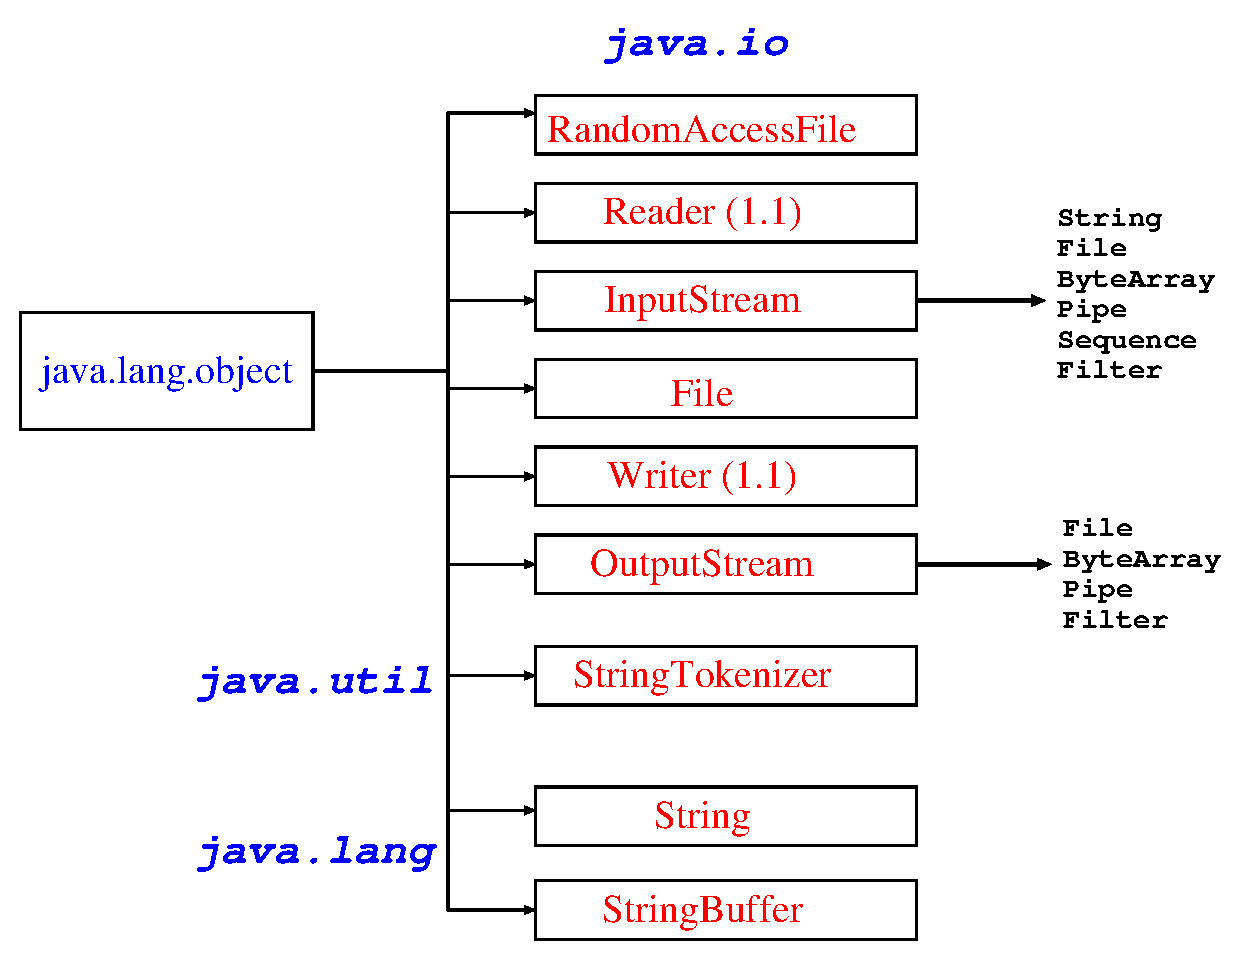
\includegraphics[width=\textwidth]{Figures/IOClasses.eps}
    \caption{Overview of the \texttt{io} package in Java 1.1 and 
      related classes.}
    \label{fig:FileIOClasses}
  \end{center}
\end{figure}
Except the \verb|Reader| and \verb|Writer| classes, all classes were
already introduced in Java 1.0. In Java 1.1 the two additional
classes just mentioned were added, because the \verb|InputStream|
and \verb|OutputStream| classes are using 8 bit characters and
the new classes use 16 bit unicode characters for international
languages support. In Java 2 only small changes have taken place
and therefore you can still stick to the Java 1.1 standard, but
should avoid using Java 1.0 I/O syntax if possible. 
This is also because the Java 1.1 Reader and Writer classes are
faster than the old ones.
Because File I/O almost always means handling strings, we have to
discuss this also in more detail. 

\paragraph{The concept of Streams}
The basic concept of input and output in Java is the \emph{stream}.
A stream is a collection of data in a certain order, which has to be
transported from a source to a sink. For example you want to
read data froma file, then you need a stream from the file, which
is the source, to a sink, which could be an array. This array can
of course be printed on screen to be read by the user. Thnis can also
be seen as a stream using the array as a source and the screen as the
sink. And really the \verb|System.out| method already familiar with
is derived froma stream (the \verb|PrintStream| class).

For any data communication from one ``point'' to another you
always have to use a stream in Java (like in C++). A nice feature
of streams is, that you can put two streams behind each other,
meaning to put the output of the first stream to the input of the 
second stream (see figure \ref{fig:ConnectingStreams}). 
\begin{figure}[htbp]
  \begin{center}
    \setlength{\unitlength}{.7cm} 
    \input{Figures/StreamsConnect.pic}
    \caption{Connecting two streams together to get advanced functionality.}
    \label{fig:ConnectingStreams}
  \end{center}
\end{figure}
This is the reason why modern programming languages
prefer to use streams to realize a very flexible input/output
API.  

You can even create very easily your own streams realizing very complex
filtering methods, but after reading this section you should be
able to understand the basics of streams and go to the online
API documentation and find your way through the classes yourself. 

\paragraph{ASCII Files}
But let us start with the most simple problem: We have an array 
of double values, for example the x coordinates of the discrete--time
random walk discussed afterwards and want to save them in a file
in the format \verb|time  x-coordinate|. To that end we need
to open a file for writing, write the array in it and close the file.

You probably would tend to look at the \verb|File| class for reading and 
writing files, but this class is only responsible for managing
files, directories and paths. We can use it to create a name
for our fiole to be created. For file access, you have to use the
\verb|Reader| and \verb|Writer| classes. So our small sample
program would look like:
\lstinputlisting{Listings_Java/FileWriteSimple.java}

First of all you realize that instead of just using the \verb|FileWriter|
class we ``pipe'' it to a \verb|BufferedWriter|, which buffers
the outgoing data between the disk and the memory. This is always
desirable and should therefore always be used. Otherwise you get
a very bad performance. Because it is inconvenient to remember all
this, we have written a convenience class in our \verb|simulation|
package. So you can have the same program, only lines 17-18 (or 19)
have to be changed to (and you have to import the simulation package,
see program \verb|FileWriteConvenience.java|.):
\begin{lstlisting}{}
    FileOut out = new FileOut( filename ); // open a buffered File stream
\end{lstlisting}
You can use a second argument to this constructor, which is a boolean
variable and indicates if ythe data should be appended to
the already existing file or not. The full syntax of the method
is therefore \verb|FileOut(String filename, boolean append)|.

Now we want to read the contents of the file back in. We use the
classes \verb|FileReader| and \verb|BufferedReader| as you may have
already guessed. The whole program looks like:
\lstinputlisting{Listings_Java/FileReadSimple.java}
Again you can use the convenience class \verb|FileIn| from the
simulation package, changing again the lines 17-18 (or 19) by:
\begin{lstlisting}{}
    FileIn in = new FileIn ( filename ); // open a File stream
\end{lstlisting}

Important remark:
\begin{quote}
Java always overwrites old files without notification as the default
behaviour! If you want to check if an old file already exists under
this name, you have to do that by yourself. If you want to append the
new data to the old one, use the second argument when creating a
new \verb|FileWriter| instance.
\end{quote}


\paragraph{Using a StringBuffer}
In the above examples and in all the \verb|System.out.println()| methods,
we make use of the concatenation operator \verb|+|. So here seems to
be the right place to discuss the fundamentals of string construction
a bit more in detail.

Often you are in the need of constructing a string from scratch, by
putting lots of small pieces (strings) together. Actually the same
problem as concatenating strings for (formatted) output. You could
always use the Lava Rocks methods, here especially the \verb|sprintf()| 
method explained in the next apragraph and in section \ref{sec:Symphony}.
But here we want to discuss how this can be implemented in  core Java.

The basic feature enabling string concatenation is the concept of a 
\verb|StringBuffer|. This is a standard class in the \verb|java.lang|
package and contains methods to manipulate strings. The \verb|String|
class itself (also in the \verb|java.lang| package) provides basic
functionality for fixed (non-changing) strings. As I already
mentioned every time you use the concatenation operator, you are
implicitly using the \verb|StringBuffer| methods. 

If you want to create a string, which contains all the output you want
to write to a file in one string, you could use a \verb|StringBuffer|.
Here is the same class as above for writing a double array to a file,
but this time we use the \verb|StringBuffer| to create a string
containing all the output and write this string to the file.
\lstinputlisting{Listings_Java/StringBufferDemo.java}
Now you have to take care of the length of the buffer yourself,
but if there is not enough space left Java automatically
enlarges the buffer itself, so you do not have to care.

Using a \verb|StringBuffer| is much faster and much less memory
extensive than just the concatenation operator, if you are
interested in the final string. If you just use it for output
it does not matter.

\paragraph{Stream- and StringTokenizer}
These two classes in the \verb|java.io| and the \verb|java.lang|
packages respectivly can be used to split up a stream of
characters or a string into words. You can define the word
separator yourself, the default is a white space. It is very
convenient for analyzing keyboard inputs or sentences.
You get the next word by using the \verb|nextToken()| method.
The \verb|StringTokenizer| is very simple and the \verb|StreamTokenizer|
is much more flexible and powerful.

\paragraph{Formatting the output in a file}
A common problem for writing files is the form of the produced
output. Like in the case of formatted screen output, you can use
one of the C language motivated \verb|printf| methods supplied by the
Lava Rocks package (see section \ref{sec:LavaRocks}). But instead
of using \verb|printf()| you have to use \verb|fprintf()| this time.

If you are a (former) C programmer, you might miss the third
output version of the formatting methods: in Lava Rocks it is also called
\verb|sprintf()|. 

A simple example of these routines would be to save
a double array, which is e.g. the x-coordinate of a particle, and 
the corresponding time in a file.
\lstinputlisting{Listings_Java/FileSaveFormatted.java}

\paragraph{Binary Files}
We are now familiar with writing ASCII files, but sometimes it is
necessary to write or read files in binary format, where the 
values are stored in the way they are kept in memory of the computer.
This makes it faster and most of the time it produces smaller
output files than using ASCII output.

The difference to other languages, where you have these two choices
too, is that in Java on all platforms the binary format is the
same, when it is saved. So here you do not have to mind using 
binary data files on different machines and operating systems as
long as you stick to Java.

All of the basic I/O classes implement writing bytes to a stream,
so you could actually use them. But there are two classes, which 
already implement the conversion of the different data types to 
a series of bytes and write these bytes to the desired stream.
The first one is \verb|DataInputStream| and the second one is
the \verb|DataOutputStream| class. They implement methods like
\verb|writeDouble()| (\verb|readDouble|), \verb|writeBoolean()|
(\verb|readBoolean()|), etc. There are also methods for
writimg strings (\verb|readLine()|) in these two classes, but
avoid them, because they do not convert the byte stream correctly
to character streams. Instead use the above discussed writer and reader
classes. 

As an example we look at the same example as above and write 100 
double variables to a file, so the file will be 800 bytes long
(on all computers and operating systems).
\lstinputlisting{Listings_Java/FileBinary.java} 
Please note that we have used unbuffered I/O here and for your
applications you should always use buffered I/O by inserting
a \verb|BufferedInputStream| (\verb|BufferedOutputStream|) between
the two streams used in the listing.

This paragraph was the way to write files introduced in Java 1.0,
the Reader and Writer classes were first introduced in Java 1.1.
There are also classes to convert the old streams to the new reader/writer
streams (classes). The \verb|InputStreamReader| class converts
an \verb|InputStream| 
to a \verb|Reader| class and the \verb|OutputStreamWriter| class 
converts an \verb|OutputStream| to a \verb|Writer| class.


\paragraph{Handling Files -- The File Class}
Sometimes you need to delete, rename or copy files or must check
if a file is already there or you have to seek in directories.
For all these problems you have to refer to the \verb|File| class 
(since Java 1.1) of
the \verb|java.io| package. Take a look at the extensive list
of methods available in this API and you will certainly find
something suitable. 

As a short example we want to discuss how show how to check if
a file with a certain filename is already available and 
how to handle directories and files therein.
\lstinputlisting{Listings_Java/FileCheck.java}

\paragraph{Direct File Access}
Since Java 1.1 
there is also a class called \verb|RandomAccessFile|, which is for
creating and accessing files directly. This means you can store
kind of data records and position the file exactly to a certain
record instead of reading the whole file sequentially. Because
in scientific applications this kind of file access is rather
seldom, we do not discuss this feature. You have to consult the
online API documentation for details. 

\paragraph{Redirecting Standard Input and Ouput}
You can redirect the standard output, input or error
to a file for example or whatever you like (since Java 1.1). 
This is of great use,
because often you run long simulations and want to save the
standard output or error to a file for later use. This can be
done easily on UNIX systems, but still you have to do it manually.
In Java you just use methods from the \verb|java.lang.System| class.
For example to redirect the standard output and error to a file
called \verb|Standard.out| of a program, use:
\lstinputlisting{Listings_Java/RedirectStandard.java}
The similar method for the standard input is called
\verb|System.setIn(InputStream)|.

\paragraph{Compressing Files}
File compression is not only important for transfering files or applets 
across the internet, it is also of concern for many scientists, who have
large data sets and have to write these sets to disk for 
postprocessing. 

Since the advent of the zlib compression library\footnote{%
\href{http://www.zlib.org}{http://www.zlib.org}} freely available under
the GNU license, it is pretty easy to use compression in your 
own programs in Fortran or C. But in Java the compression library is 
already made available in the standard Java API \verb|java.util.zip|.
As the name suggests not only the zlib compression algorithm used
in the famous GZIP program -- mostly used on UNIX systems using the
\verb|.gz| ending -- but also the algorithm of the famous zip
program -- mostyl used on Windows based systems and has the ending
\verb|.zip| -- is available in Java directly.

The only drawback is that it is implemented on top of the old
Java 1.0 I/O API and sometimes you have to mix the old Java 1.0
and the new Java 1.1 I/O syntax. 

The most easy interface is the GZIP one, so for most applications you 
should use GZIP. The Zip interface allows for multiple program 
compression in one file, but it is more cumbersume to use. Because
most of the time you have to compress a single stream of data, we
explain only the GZIP interface.

Let us discuss the probelm ofg saving an array to a file again, but
this time we want to store them compressed as a GZIP file.
\lstinputlisting{Listings_Java/GZIPSaveArray.java}
The first part stores it as a binary GZIP file \verb|test.bin.gz|
and you will see that it
does not save a lot of memory, because we are storing an array with random
numbers, which is already (almost) best represented by the binary
format. The second part produces an ASCII GZIP file \verb|test.asc.gz|,
which is much smaller than the uncompressed file. You can check this by
using the GZIP utility and uncompress the files. 

Reading of GZIP files works the same, you just have to use
the \verb|GZIPInputStream()| constructor and all the file I/O works
like usual file handling.

We have also implemented convenience classes for these complicated
structures to open a GZIP file for writing and reading. They are
called \verb|GZFileOutBin()| (\verb|GZFileOutAscii()|) and
\verb|GZFileInBin()| (\verb|GZFileInAscii()|) and are used like
the ones without compression. You can also take a look at the
program \verb|GZIPReadArray.java|.

\paragraph{Reading Files into Applets}
Because of security reasons there is (almost) no way of reading files or
writing files from within an applet. One way of doing it would be
to use the security features of Java. In this case the browser has 
to tell the applet explicitly that it is allowed to do file I/O. This
can be accomplished by signing an applet, prepared in a jar file. Then
the browser can check the signature and if the browser setup allows
file I/O for this signature it works.

A second way would be to use the network features of Java and
access a file from a FTP server, probably the same computer
the applet was coming from. Of course there is still the problem
of a password to be transmitted unsecurely to the FTP server, but
it is fairly easy to setup. The code to use is a freely available
program called \verb|LinLyn.java|. We have included the code in
our simulation package. The documentation is included in the Java file
or you can study the simulation package documentation. 

%%%%%%%
\subsection{Exception Handling in Java}
We have made extensive use of exceptions in the last section, but
now we have to understand what we did there. Exceptions are
``thrown'' if an exceptional condition or error occurs in a part
of a Java program. This can be a division by zero, a file not
found error or something else, which the JVM does not know 
how to handle. So it is up to you to write code, which takes
care of unusual conditions, which is called catching an exception 
-- the most common situations are already
caught by the standard Java implementation. 

If a piece of code produces an exception it is checked if the
code block surrounding the exception producing point is able
of handling the exception. If not, the exception is propagated
up to the next higher (calling) code block (method, class, etc.).
If none of the code up to the main method catches the exception,
an error message is shown on the command line and the program stops
with a stacktrace showing the last commands executed. This propagation
is a great simplification, because you can catch all of the exceptions
in one place and not distributed through the whole class hierarchy.

The exception handling is located in the \verb|java.lang.Throwable| class.
Exceptions are objects and there are two types: Errors and Exceptions.
Errors are usually not recoverable and the program has to exit with
an error message. From exceptions you can recover, e.g. 
``Array out of Bounds'', or ``IO Exception'', etc. The exceptions,
which are automatically caught are the \verb|RuntimeExceptions|.

The way of handling exceptions is easily seen in the above examples
about file I/O. You put the code, which can throw an exception in a
\verb|try { }| clause and use the \verb|catch() {}| clause afterwards
to define what has to be done, if an exception occurs in the try block.
\begin{verbatim}
try {
   // Code which throws exceptions.
} catch ( java.lang.Throwable e ) {
   // Code which catches/recovers from exceptions.
} finally {
   // Code which should be executed, no matter if an exception
   // occured or not, before global catching of the exceptions 
   // takes place.
}
\end{verbatim}
The \verb|java.lang.Throwable| keyword in the catch clause has to be
exchanged by one of the exceptions in table \ref{tab:Exceptions}. 
\begin{table}[htbp]
  \begin{center}
    \begin{tabular}{lcp{.6\textwidth}}
      Exception name & RTE & Ocurrence/Reason \\\hline
      IOException & N & Some IO problem (has lots of subclasses). \\
      ArrayIndexOutOfBoundsException & Y & array is out of bounds \\
      ArtihmeticException & Y & Integer division by zero \\
      NullPointerException & Y & If a \verb|null| instead of an object is used\\
      NegativeArraySizeException & Y & if you trie to create a negative sized array\\
    \end{tabular}
    \caption{Some of the important exceptions in the 
      \texttt{java.lang.Throwable} class. A detailed list is in the 
      API documentation. RTE means \texttt{RuntimeException} and therefore
      do not have to be catched.}
    \label{tab:Exceptions}
  \end{center}
\end{table}

Instead of explicitly catching exceptions you can also just
write \verb|throws IOException| after the class definition, before
the actual code. Then the exceptions are handed to the next higher 
instance and if there is no calling class anymore an error is
displayed. With this you can propagate all your exceptions to the
parent class of all of the classes and catch the exceptions there.

If you ask how do you know what exceptions to catch (if some of the
code is not written by you or is very complex), there are only
two possibilities: read the whole code and look for exeptions, which
can be thrown by it or wait for the exceptions to occur on the
standard output. 

You can even use your own exceptions very easily by using the keyword
\verb|throw| and your own name of an exception. That is an easy way
of handling exceptional conditions in your own code, like energy
turns zero or step size/accuracy gets too large, e.g.
\begin{verbatim}
  try {
       energy = newEnergy(energy);
       if (energy == 0 ) {
           throw  new EnergyZeroException(); 
       }
  } catch (EnergyZeroException e) {
       // do something about zero energy
  } catch (OtherExceptions e) {
       // maybe another exception to be caught
  } finally {
       // Always do something here, even if a certain exception
       // has been thrown, but not catched yet
  }
\end{verbatim}


%%%%%%%%%%%%
\subsection{The Discrete--Time Random Walk}
A drunkard leaves a pub. His house is at the end of a straight
street. Each time  he moves he walks one
step to the direction of his home  or one step in the opposite direction
with equal probability. The question we want to consider in this 
subsection is: What is the probability for the drunkard to be at 
home in $r$ steps? 

In a more formal language we want to associate with each step
a stochastic variable $X_i$ ($i=1,\ldots,r$) assuming only the 
values $+1$ and $-1$ with probability $1/2$ each. If he starts at
$n=0$, all possible positions are integers $-\infty < n <
\infty$. The position after $r$ steps will be
\begin{equation*}
Y = X_1 + X_2 + \cdots + X_r.
\end{equation*}
It is easy to check that $\langle Y \rangle = 0$ and since
the steps are mutually independent
\begin{equation*}
\langle Y^2 \rangle = r \langle X^2 \rangle = r.
\end{equation*}
The above relation expresses the very typical behaviour of a 
diffusive process: The mean squared displacement is proportional 
to the number of steps. To put it differently the variance of the 
mean of the velocity tends to zero  for long times
\begin{equation*}
\left\langle \left( \frac{Y}{r}\right)^2\right\rangle =
\frac{1}{r} \longrightarrow 0 \quad \text{as} \quad 
   r \longrightarrow \infty.
\end{equation*}

In order to find the probability distribution of $Y$ we make use
of the characteristic function
\begin{equation*}
G_Y(k,r) = [G_X(k)]^r = [\frac{1}{2}\exp(ik) + 
                   \frac{1}{2}\exp(-ik)]^r.
\end{equation*}
The probability that $Y$ has the value $n$ is the coefficient
of $\exp(ink)$
\begin{equation*}
p_n(r) = \frac{1}{2^r} {r \choose {\frac{(r-n)}{2}}}.
\end{equation*}

In order to make clearer these concepts we want to write a program 
to simulate the random walker in discrete time steps. The program
is called {\sf rwdt} and its listing can be seen below.

\subsubsection{Listing of the program rwdt.m}

\inputlisting{./Listings/rwdt.m}

In the program we have obviously to generate an integer valued random 
variable which can assume with equal probability the values $+1$ 
and $-1$. One way of generating an $n$--dimensional vector $x$ of 
such random numbers is
\begin{verbatim}
x = sign(rand(n,1)-0.5)
\end{verbatim}
We run the program for 1000 steps, i.e., we choose the parameter 
$nstep=1000$.
Two realizations of the one--dimensional random walk can be seen 
in Figs. (\ref{F_RWDT_1}) and (\ref{F_RWDT_2}). 
\begin{figure}
\label{F_RWDT_1}
\includegraphics[width=10cm]{./Figures/f_rwdt_1.eps}
\caption{One realization of a one--dimensional random walk.}
\end{figure}

\begin{figure}
\label{F_RWDT_2}
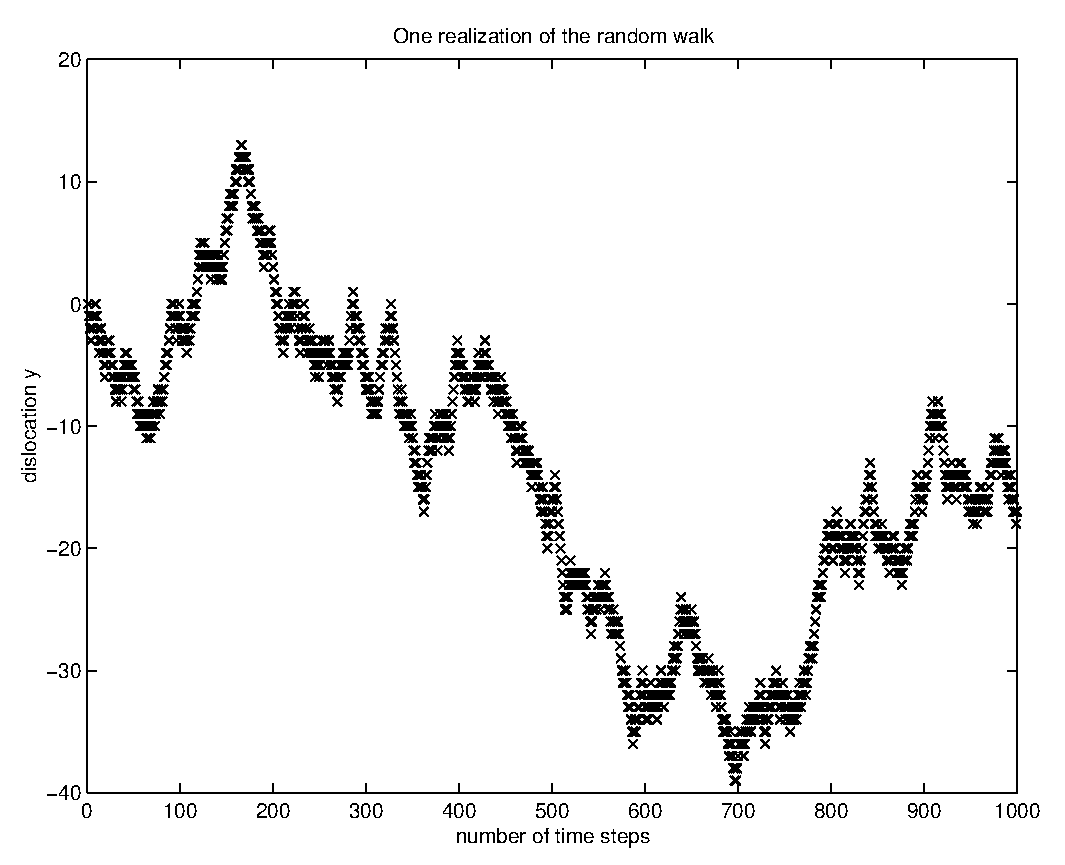
\includegraphics[width=10cm]{./Figures/f_rwdt_2.eps}
\caption{Another realization of a one--dimensional random walk.}
\end{figure}

In order to check the theoretical prediction that the mean square
displacement is proportional to the number of steps we generalize the program
{\sf rwdt} to allow for the generation of more realizations and 
the estimation of the mean value and variance. The new program is called 
{\sf rwdtn} and generates {\sf nreal} realizations of the 
stochastic process.
Its listing can be seen below.

\subsubsection{Listing of the program rwdtn.m}
\inputlisting{./Listings/rwdtn.m}
We run the program for $nstep=100$ and $nreal=1000$. The estimated
mean value of 0.274 and the estimated variance of 103.304 are in quite
good agreement with the theoretical expected vales of 0 nd 100, respectively.
It is interesting to look also at the distribution of the end points of 
the random walk. This can be seen in Fig. (\ref{F_RWDTN}).
\begin{figure}
\label{F_RWDTN}
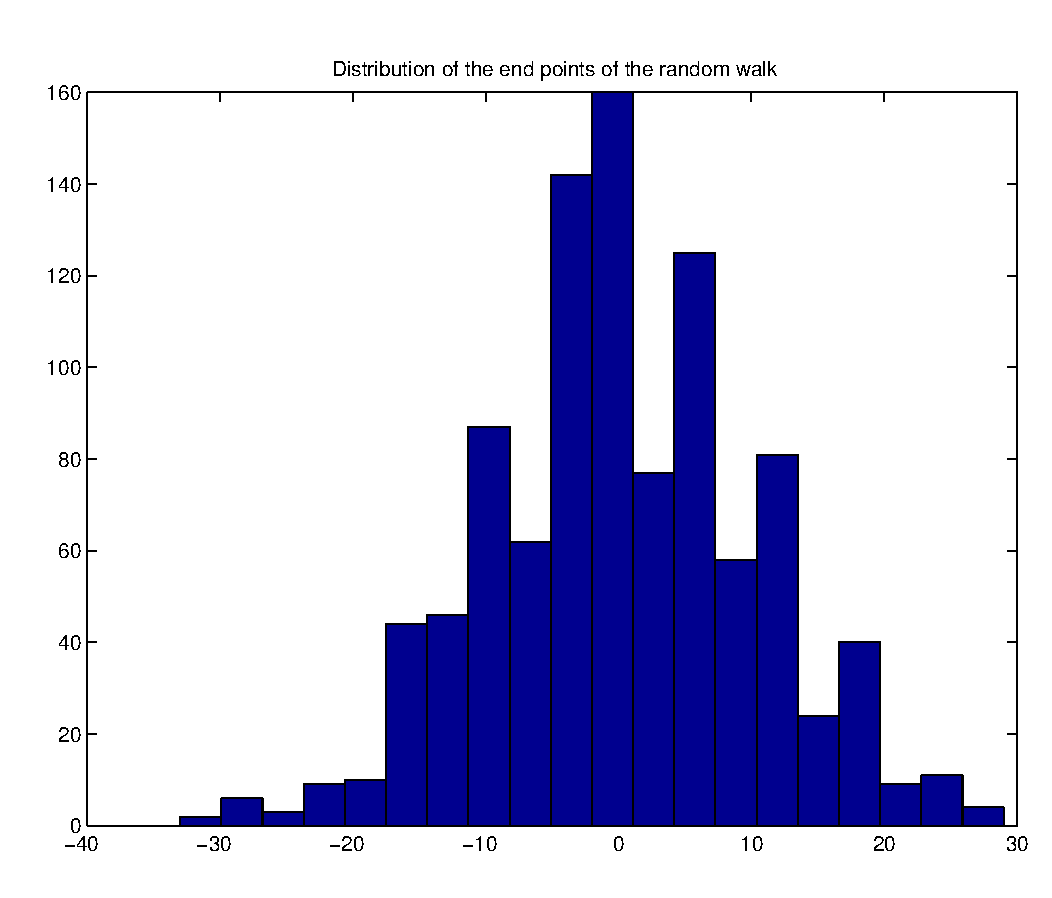
\includegraphics[width=10cm]{./Figures/f_rwdtn.eps}
\caption{The distribution of the end--points of the one--dimensional 
random walk. the program {\sf rwdtn} was run for nstep=100 and 
nreal=1000.}
\end{figure}
\subsection{Generation of Gaussian Random Numbers}
As a simple demonstration of the central limit theorem we want to 
generate Gaussian distributed random numbers by adding uniformly 
distributed ones.

We know that uniformly distributed random numbers on the interval
$[0,1)$ have $p(x) =1$ for $x\in[0,1)$. Then it is easy to show 
that 
\begin{equation*}
\langle X\rangle = \frac{1}{2}
\end{equation*}
and
\begin{equation*}
{\rm Var}(X) = \int_0^1 x^2 dx - \langle X^2\rangle = \frac{1}{3} 
        -\frac{1}{4} = \frac{1}{12}.
\end{equation*}
Now let us consider the transformed random variable $X'$
\begin{equation*}
X' = (X - \frac{1}{2})\sqrt{12} \sigma
\end{equation*}
which has mean $0$, variance $\sigma^2$, and is uniformly 
distributed on the interval 
$[-\frac{1}{12} \sqrt{12} \sigma, \frac{1}{12} \sqrt{12} \sigma].$
Let us now draw $N$ such random numbers $X'_1,\ldots, X'_N$
and let us construct
the new stochastic variable $Z$
\begin{equation*}
Z= \frac{1}{\sqrt{N}} (X'_1 + \ldots + X'_N).
\end{equation*}
Then the central limit theorem states that the variable $Z$ is a Gaussian
variable with mean $0$ and variance $\sigma^2$.

With the help of the program {\sf cltgen} we want to demonstrate 
that already for $N=12$ we get Gaussian distributed random numbers
in a very good approximation.

\subsubsection{Listing of the program cltgen.m}
\inputlisting{./Listings/cltgen.m}

In Fig. (\ref{F_CLTGEN}) we see the distribution of the Gaussian 
random numbers generated with the help of the program {\sf 
cltgen}. The number of random numbers $Z$ was chosen to be 1000.
\begin{figure}
\label{F_CLTGEN}
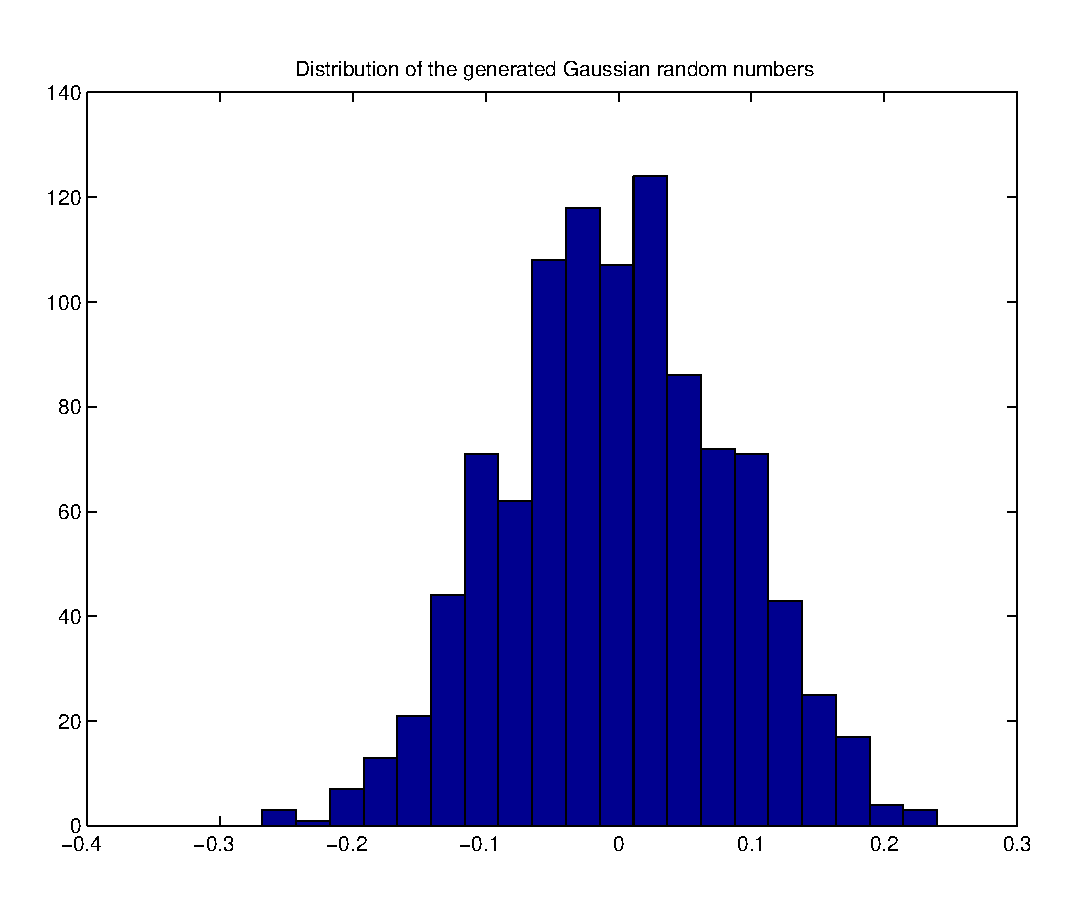
\includegraphics[width=10cm]{./Figures/f_cltgen.eps}
\caption{The distribution of the Gaussian random numbers generate
with the help of the program {\sf cltgen}. The number of random numbers 
drawn was chosen to be $n=1000$.}
\end{figure}

\subsection{Estimation}
{\em Experimental data are random numbers!} An experiment provides
realizations of some random variable $X$. We call an $N$--fold
realization of $X$ a sample of size $N$. It is of fundamental
importance to distinguish between the estimate for the mean and the
variance made on the basis of the sample, which we will denote by $m$
and by $s$, respectively and the corresponding quantities for the
(infinite) underlying population, the ensemble.

Of course, estimates should be unbiased, i.e., for very large samples
the estimate based on the sample size $N$ should converge to the
ensemble averages.

\subsubsection{Mean Values}
Let us consider $N$ copies $X_1, \ldots, X_N$  of a random variable
$X$ and let us build the new stochastic variable
\begin{equation*}
Z = \frac{1}{N}(X_1 + \cdots + X_N).
\end{equation*}
$Z$ is the mean value of the $N$ realizations. Assuming that the $X_i$
are uncorrelated we obtain for the cumulants of $Z$
\begin{equation*}
\kappa_n(Z) = \frac{1}{N^n} \sum_{i=1}^N \kappa_n(X_i) =
      N^{-n+1}  \kappa_n(X).
\end{equation*}
In particular we have
\begin{eqnarray*}
\kappa(Z) & = & \langle Z \rangle = \langle X \rangle \\
\kappa_2(Z) & = & {\rm Var}(Z) = \frac{1}{N} \kappa_2(X) = \frac{1}{N}
                  {\rm Var}(X) \\
\kappa_n(Z) & = & O(N^{-2}) \;\;\; {\rm for} \;\; N>2.
\end{eqnarray*}
In other words the mean value of $Z$ is a random variable with a
distribution which has the same mean value as $X$, but with a variance
which is smaller by a factor of $N$. Up to terms of the order
$O(N^{-2})$ the distribution of $Z$ is Gaussian.

\subsubsection{Estimating Mean and Variance}
Let us consider to have the sample $x_1, \ldots, x_N$. A natural
estimator of the mean value $\mu$ is the sample mean
\begin{equation*}
m= \frac{1}{N} \sum_{i=1}^N x_i.
\end{equation*}
An estimate for the variance could, in analogy, naturally assumed to
be
\begin{equation*}
  \bar{\sigma}^2 = \frac{1}{N} \sum_{i=1}^N (x_i -m)^2.
\end{equation*}
Unfortunately, the above estimator is biased, because we make use of
the already known $m$ instead of the unknown $\mu$. As can easily be
seen
by adding and subtracting $\mu$ in each term in the above equation we
get
\begin {eqnarray*}
 \bar{\sigma}^2 &=& \frac{1}{N} \sum_{i=1}^N [x_i - \mu -(m-\mu)]^2 \\
                & = & \frac{1}{N} \sum_{i=1}^N (x_i - \mu)^2
                              -2(m-\mu)\frac{1}{N} \sum_{i=1}^N (x_i
                                   - \mu)
                           +(m-\mu)^2 \\
               & = & \frac{1}{N} \sum_{i=1}^N (x_i - \mu)^2 - (m-\mu)^2.
\end{eqnarray*}
Now, by taking expectation values averaging over an infinity of samples
of size $N$ we have
\begin{eqnarray*}
E[\bar{\sigma}^2] &= & E\left[\frac{1}{N} \sum_{i=1}^N (x_i - \mu)^2
                                \right]
            - E\left[(m-\mu)^2 \right] \\
       & = & \sigma^2 - \sigma_m^2.
\end{eqnarray*}
If we assume, that there are no correlations we have $\sigma^2_m=
\sigma^2/N$, an unbiased estimate of $\sigma^2$ is
\begin{equation*}
s^2 = \frac{N}{N-1} \bar{\sigma}^2 = \frac{1}{N-1} \sum_{i=1}^N 
      (x_i - m)^2.
\end{equation*}
In computations, if the sample is large, rounding errors can be large
because $(x_i - m)$ is small. In
these cases it is convenient to use the 
"corrected two--pass algorithm" for $s^2$
\begin{equation*}
s^2 = \frac{1}{N-1} \left\{ \sum_{i=1}^N 
      (x_i - m)^2 - \frac{1}{N} \left[\sum_{i=1}^N 
      (x_i - m) \right]^2  \right\}.
\end{equation*}
The function of the additional second term which would be identically
equal to zero if $m$ were exact is to correct the rounding errors of
the first term \cite{PRESS}.

\subsubsection{Confidence Levels}
It is important to have also a quantitative characterization of the
goodness of the estimation. To this end we assign to every 
estimation a certain confidence interval, which is to be chosen in 
such a way that the true value lies within this interval at some
predetermined level of confidence. Since we know, by virtue of the
central limit theorem, that the mean value is Gaussian distributed
a criterion for the error can be directly derived from the 
geometric properties of the distribution. Assuming that the
mean value is $m$ and that the standard deviation is
$\sigma_m$ then the probability to find the true value in the
interval $[m-\sigma,n+\sigma]$ is given by the surface 
under a normal probability density
between  $\mu-\sigma_m$ and $\mu + \sigma_m$
\begin{equation*}
{\rm Prob}(\mu \in [m-\sigma,n+\sigma]) =
\int_{m-\sigma}^{m+\sigma} \frac{1}{\sigma \sqrt{2\pi}}
       \exp\left( - \frac{(x-m)^2}{2\sigma^2}\right)
       = 0.683.
\end{equation*}
Thus, in $68.3 \%$ of
samples a value lying within $\pm \sigma_m$  of the population mean
$\mu$ would be found. Conversely, there is $68.3 \%$ probability that
the interval $[m-\sigma_m, m+\sigma_m]$ contains the population mean.

In general we have...

\section{Beyond this Chapter}

%%%%%%%%%%%%%%%%%%%%%%%%%%%%%%%%%%%%%%%%%%%%%%%%%%%%%%%%%%%%%%%%%%
\section{Exercises}

\begin{Ex}
\label{Random-Number_Generator_Check}
\textbf{Random-Number Generator Check \cite[]{knuth2:81}} \\
To test the random number generator of Matlab, we calculate the first
10 moments of the distribution generated from \texttt{rand()}.
Compare these with the exact results for a uniform distribution.

Plot a histogram to check for a uniform distribution.

Use the Poker-Test for testing \texttt{rand}: Create many series of 5
random numbers between 1 and 13. Then count the fractions of hands
with two, three and four identical (numbers) cards. Compare the
result with the predictions:
\begin{center}
  \begin{tabular}{lrr}
hand & number of ways& probability\\\hline
all different (no pair) & 1,302,540 & 0.50117739\\
two of a kind & 1,098,240 & 0.42256903\\
three of a kind & 54,912 & 0.021128451\\
four of a kind & 624 & 0.000240096 \\\hline
Total number of possibilities & 2,598,960 & 1
\end{tabular}
\end{center}
For a rigorous check you have to use the chi-squared test for
your results. If you are interested, take a look at the book of D. Knuth.   
\end{Ex}

\begin{Ex}
\label{Galton_Board}
\textbf{Galton Board and Pascal Triangle \cite[]{whitney:90}} \\
Write a program to simulate a Galton Board on the computer.

\begin{center}
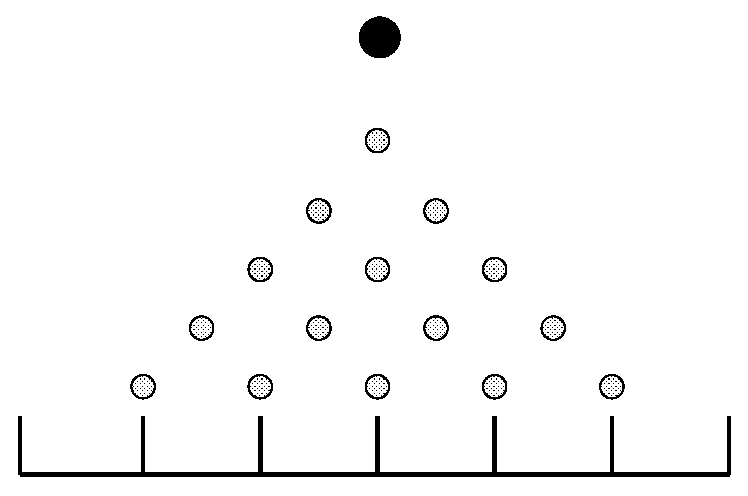
\includegraphics[height=4cm]{Galton_Board.eps}
\end{center}

That is a device where you introduce a ball at the top. The ball
falls down towards the bottom, bouncing off the pins to the right
or left at each level. The only random effect is the bouncing at
the pins at each level. The probability of bouncing to the right or
left is always $0.5$. Therefore it is a simple model for a symmetric
random walk in one dimension.

How can you extract the number of ways to get to one particular
box at the end of the board out of the estimated probabilities above?
What is the connection to the Pascal Triangle?

Change the program to simulate a asymmetric random walk in one
dimension.
\end{Ex}

\begin{Ex}
\label{Standard_Deviation}
\textbf{The Standard Deviation } \\
Compare the four possibilities to calculate the standard deviation
(or the variance):
\begin{enumerate}
\item using the definition: \\
  $$\sigma^2 = \frac{1}{N-1} \sum_{i=1}^N \left( x_i-\overline{x} \right)^2,
    \quad \overline{x} = < x > = \frac{1}{N} \sum_{i=1}^N x_i .$$
\item using the moments: \\
  $$ \sigma^2 = < x^2 > - < x >^2, \quad < x^2 > = \frac{1}{N} 
     \sum_{i=1}^N x_i^2 .$$
\item using the formula (\cite[]{scariano:91}):
  $$ \sigma^2 = \frac{1}{N^2} \sum^N_{\substack{i=1 \\ i<j}} 
      \left( x_i-x_j\right)^2.$$
\item using the corrected two-pass formula \cite[]{recipes}:
  $$ \sigma^2 = \frac{1}{N-1} \left\{\sum_{i=1}^N (x_i-\overline{x})^2
     -\frac{1}{N} \left(\sum_{i=1}^N(x_i-\overline{x}) \right)^2 \right\}.$$
\end{enumerate}
The first and the second method require the computation of the first or
the first and the second moments. The third moment doesn�t require any
precomputed values at all and the last one uses again only the first moment.
The last one corrects for the roundoff errors, encountered when using large
sample sizes. The last one is analytically exact only if $\overline{x}$
would be exact. 

Write a program including all four methods and compare the results.
Find out which method the Matlab function \texttt{std} uses.
Check the calculation with a uniform, a normal and a Cauchy (Lorentz)
distribution. Can you find an example where the two-pass algorithm
is superior to the other ones?

By the way, the variance is not the only value to estimate the
spreading of a sample. Statisticians often use the estimate
$$ \text{adev}\, = \frac{1}{N} \sum_{i=1}^N \left| x_i - \overline{x}\right|$$
as a measure for the distribution width around the mean value.
\end{Ex}

%%%%%%%%%%%%%%%%%%%%%%%%%%%%%%%%%%%%%%%%%%%%%%%%%%%

{\bf Exercise 2} Random variable transformation theorem: (a) Consider 
the linear transorm of X: Y=bX+c. (b) the log--normal 
distribution.
Lit. Gillespie, Am. J. Phys. 51 (1983) 520.
lichkeitstheoretische Grundbegriffe; typische 
Verteilungen (Poisson, Gauss, Binomial); 

%%%%%%%%%%%%%%%%%%%%%%%%%%%%%%%%%%%%%%%%%%%%%%%%%%%%%%%%%%%%%%%%%%


\bibliographystyle{peter}
\bibliography{V_98,simulit}

%%% Local Variables: 
%%% mode: latex
%%% TeX-master: t
%%% End: 


%%% Chapter 3 
%%%%%
%%%%% Chapter 3
%%%%%
\chapter{Simple Sampling of Probability distributions Using Random numbers}
This Chapter is devoted to the following question: How can we 
generate sequences of random numbers which are distributed 
according to some given distribution?

A simple answer to this question would be to exploit some 
intrinsically random physical process. For example, one could 
record a sequence of the decay times of some radioactive substance 
and use this truly random sequence of numbers in a Monte--Carlo
simulation. Although tables of millions of such true random 
numbers exist in practice this approach turns out not to be very
practical. Monte--Carlo simulations need very long sequences of 
random numbers, so that we have to find more efficient ways to 
generate them. In order to satisfy this requirement we have to 
be satisfied with the use of so--called pseudo--random numbers.
Pseudo--random numbers are generated numerically with the help of 
some simple algorithm on some computer. Consequently, they are
reproducible. This is, however, not a drawback. In fact, the 
reproducibility may be very useful if we want to check our 
simulation algorithms. 

Pseudo--random numbers are, the name already underlines it, not 
truly random. However, their statistical properties are very 
similar to the statistical properties of truly random numbers. So, 
for all practical purposes pseudo--random numbers appear to be 
random. Let us now see how such pseudo--random numbers can be 
generated.

\section{The generation of uniformly distributed random numbers}
We will begin with the generation of uniformly distributed random 
numbers on the interval $[0,1)$. In the following we will often 
omitt the prefix pseudo. 

The best known algorithm for the generation of uniformly 
distributed random numbers is the linear congruential method, 
which given an initial integer "seed" value $I_1$ produces random 
integers recursively from the formula
\begin{equation*}
I_{n+1} = (aI_n +c) \mod M,
\end{equation*}
where $a$, $c$, and $M$ are integer constants which have to be 
chosen appropriately. 
The randomness of the above algorithm results from the fact that 
after some multipications with $a$ the result exceeds $M$ and is 
consequently truncated. Since the integers $I_n$ lie between 1 and 
$M$ a random number $R$ uniformly distributed 
between 0 and 1 is obtained as
\begin{equation*}
R = \frac{I_n}{M}.
\end{equation*}
Unfortunately, MATLAB does not have integer arithmetic so the above algorithm 
has to be implemented using the {\sf rem} (remainder) function 
instead of the modulo function. A corresponding code could be
\begin{verbatim}
I(n+1) = floor( rem(a*I(n) + c,M) ).
\end{verbatim}
In order to get familiar with this algorithm we want to generate a 
sequence of pseudo--random numbers for the following parameters:
we choose the multiplier to be $a=$, the increment $c=3$, and the 
modulo $M=8$. Obviously the longest period of random numbers will
have the length 8. The generation of the random sequences will
be achieved with the program {\sf trandom1}.

\subsubsection{Listing of the program trandom1.m}
%%%%% trandom1 %%%%%%%%%%%%%%%%
\begin{verbatim}
% trandom1 - Program to demonstrate the generation of random numbers
% using the linear congruential method
clear; help trandom1 %clear the memory and print header
seed = input('Enter the seed (1) - ');
m = input('Enter the modulus (8) - ');
a = input('Enter the multiplier (5) - ');
c = input('Enter the increment (1<=c<7) - ');
% Set starting value
R(1) = seed;
% Generate vector of m random numbers
for j=1:m
   R(j+1) =floor(rem(a*R(j)+c,m));
end
%R=R/M;
disp('The generated series is:')
disp(R)
plot(R,'x')
title('The series of generated random numbers');
xlabel('Term, i'); ylabel('Value');
\end{verbatim}
%%%%%%%%%%%%%%%%%%%%%%%%%%%%%%%%%%%%%%%%%%%%%%%%%%%%%%%%%%%%%%%

Run with the above parameters the program generates the sequence
\begin{equation*}
1, 0, 3, 2, 5, 4, 7, 6, 1, 0, 3, 2 \ldots
\end{equation*}
which has also been plotted in Fig. (\ref{F_TRANDOM1}).
\begin{figure}
\label{F_TRANDOM1}
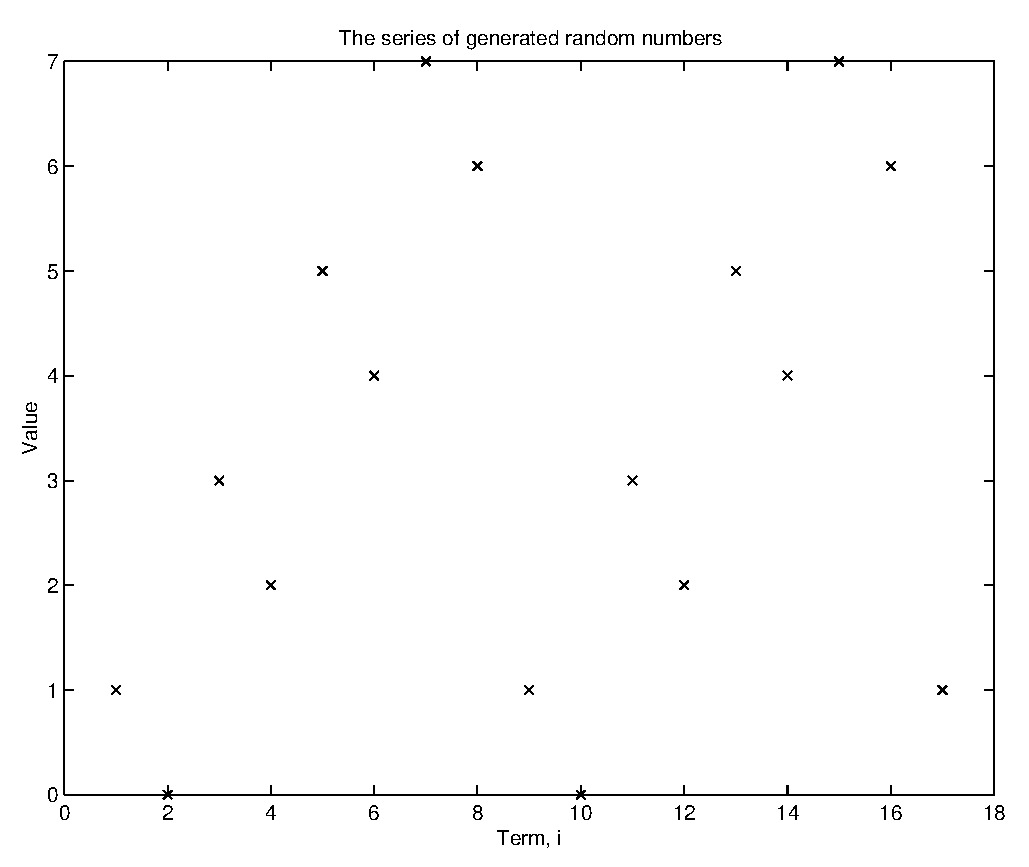
\includegraphics[width=10cm]{./Figures/f_trandom1.eps}
\caption{Successive values in a series of random numbers generated
for a=5, c=3, M=8. Note that the even numbers are always one less 
then the odd ones!}
\end{figure}
It might be instructive to run the program keeping the multiplier 
and the modulo fixed while changing the increment. The result of 
these runs are summarized in Table \ref{T_LCG}.

\begin{table}
\label{T_LCG}
\caption{Series of random numbers for the linear congruential 
generator of the form $I_{n+1} = (5I_n +c) \mod 8$}
\begin{tabular}{ccc} \hline
c &  $I_n$ & Period  \\ \hline
1 & 1,6,7,4,5,2,3,0 & 8 \\
2 & 1,7,5,3,1,7,5,3 & 4 \\
  & 4,6,0,2,4,6,0,2 & 4 \\
3 & 1,0,3,2,5,4,7,6 & 8 \\
4 & 1,1,1,1,1,1,1,1 & 1 \\
  & 2,6,2,6,2,6,2,6 & 2 \\
  & 3,3,3,3,3,3,3,3 & 1 \\
  & 4,0,4,0,4,0,4,0 & 2 \\
  & 5,5,5,5,5,5,5,5 & 1 \\
  & 7,7,7,7,7,7,7,7 & 1 \\
5 & 1,2,7,0,5,6,3,4 & 1 \\
6 & 1,3,5,7,1,3,5,7 & 4 \\
  & 2,0,6,4,2,0,6,4 & 4 \\
7 & 1,4,3,6,5,0,7,2 & 8
\end{tabular}
\end{table}
It is evident that a wrong  choice of the constants leads to a 
very poor random sequence.

It can be shown that (Knuth)  that in the case $c=0$ the full 
period, 1 to $M-1$ can be achieved by choosing $M$ as aprime 
number and for $a$, a primitive element modulo $m$, i.e., for all 
prime divisors, $p$, of $(M-1)$, 
\begin{equation*}
a^{(M-1)/p} {\rm mod} M \ne 1.
\end{equation*}
For the case of $c\ne 0$ the full period is obtained if the 
following three conditions are satisfied:

(i) $c$ and $M$ are relatively prime,

(ii) $a {\rm mod} p = 1$ for each prime factor $p$ of $M$,

(iii) $a {\rm mod} 4 = 1$ if 4 divides $M$.

It is evident that the greater the modulus the longer the period.
For example the MATLAB random number generating function uses
\begin{equation*}
a= 16807; c=0; M=2^{31}-1.
\end{equation*}
This chioce has been suggested by Park and Miller (Lit. Press).
The period of the generator is $2^{31}-2 \approx 2.1 \times 10^9$.
Another poupular popular random generator uses
\begin{equation*}
a= 65539; M=2^{31}-1; c=0,
\end{equation*}
and will be used in the following program {\sf trandom2.m}. There 
we will draw a number $n=xxx$ of random numbers using the linear 
congruential method. In the program we will check the quality of 
the generator by plotting the 1D, 2D, and 3D distribution of the 
pseudo--random numbers. The results of the test can be seen in 
Figs. (\ref{F_TRANDOM2_1}), (\ref{F_TRANDOM2_2}), 
(\ref{F_TRANDOM2_3}), and (\ref{F_TRANDOM2_4}).



\subsubsection{Listing of the program trandom2.m}
\begin{verbatim}
% trandom2 - Program to test random number generators
% The program makes use of the random number generator random1
clear; help trandom2; % clear memory and print header
% Enter dimension of random vector
n= input('Enter value of n-'); % 
% generate random vector
R1=random1(n);
% plot random vector
plot(R1)
title('random numbers'); xlabel('random variable');
disp('Histogram: press any keyboard key');
pause;
% plot histogram of random numbers
x=(0.05:0.1:0.95);
[m,xout] = hist(R1,x);
bar(xout,m)
xlabel('random number');
title('1D distribution: Histogram');
disp('2D plot: press any keyboard key');
pause;
% 2D plot: correlation of consecutive numbers
R2x=R1(1:2:n-1);
R2y=R1(2:2:n);
plot(R2x,R2y,'x')
title('2d distribution')
disp('3D plot: press any keyboard key');
pause;
% 3D plot: correlation of consecutive numbers
R3x=R1(1:3:n);
R3y=R1(2:3:n);
R3z=R1(3:3:n);
%R3=random1(n,3);
plot3(R3x,R3y,R3z,'x')
title('3D distribution');xlabel('Random number');
\end{verbatim}

\subsubsection{Listing of the function {\sf random1}}
%%%%%%%%%%%%%%%%%%%%%%%%%%%%%%%%%%%%%%%%%%%%
\begin{verbatim}
function R = random1(n)
% function to generate random numbers
a=65539;
M=2^(31)-1;
R(1) = 12345678;
for j=1:n-1
%   for i=1:n-1
   R(j+1) =floor(rem(a*R(j),M));
%end
end
R=R/M;
\end{verbatim}

\begin{figure}
\label{F_TRANDOM2_1}
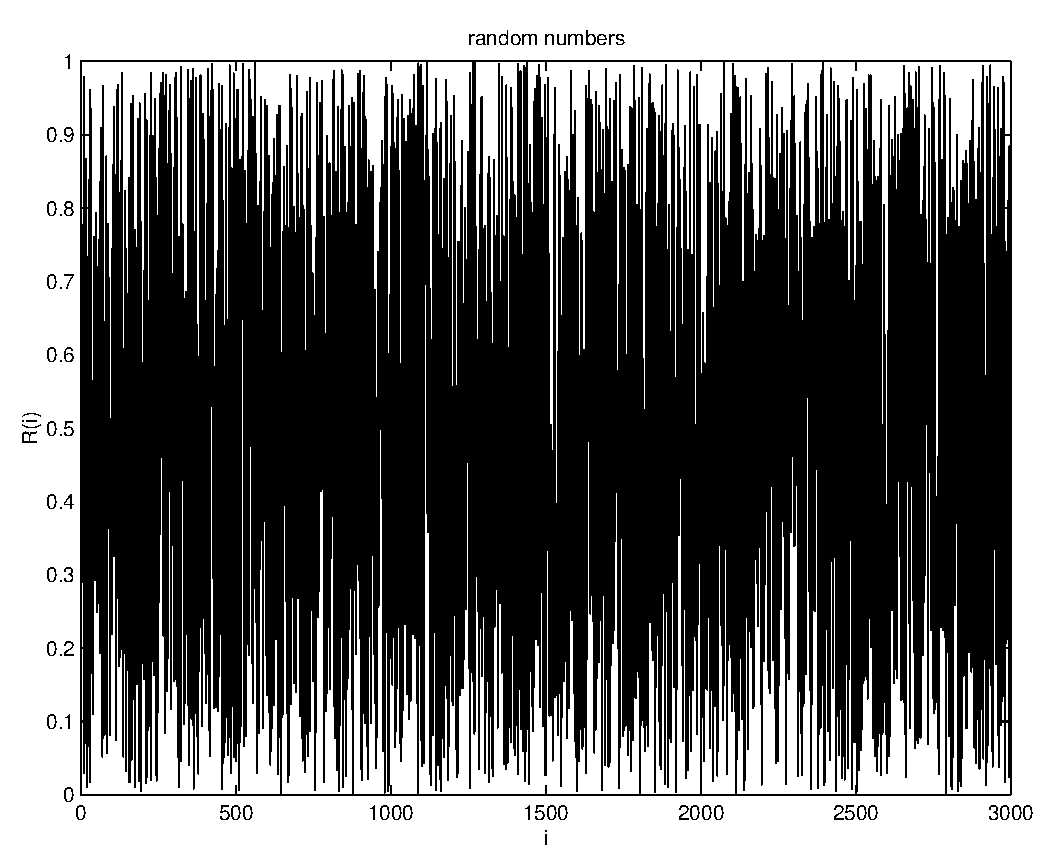
\includegraphics[width=10cm]{./Figures/f_trandom2_1.eps}
\caption{Successive values in a series of 3000 random numbers generated
for $a=65539$, $c=0$, $M=2^{31}-1$.}
\end{figure}

\begin{figure}
\label{F_TRANDOM2_2}
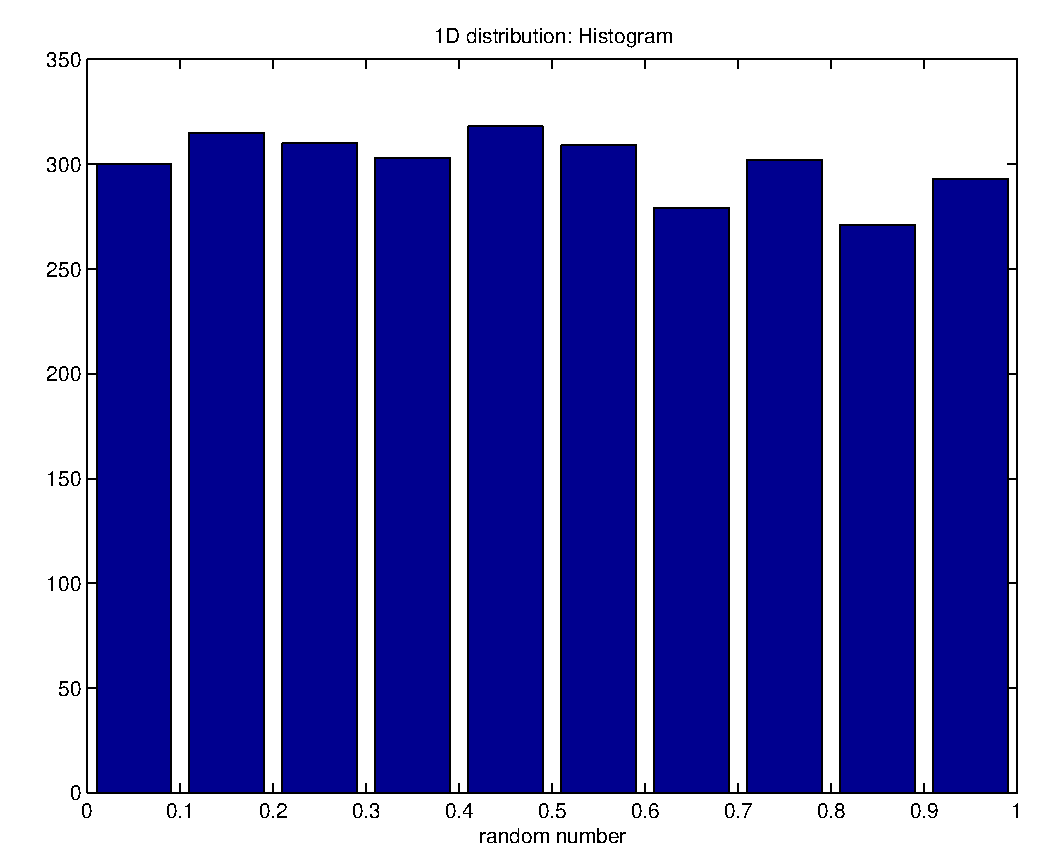
\includegraphics[width=10cm]{./Figures/f_trandom2_2.eps}
\caption{Histogram for a series of 3000 random numbers generated
for $a=65539$, $c=0$, $M=2^{31}-1$.}
\end{figure}

\begin{figure}
\label{F_TRANDOM2_3}
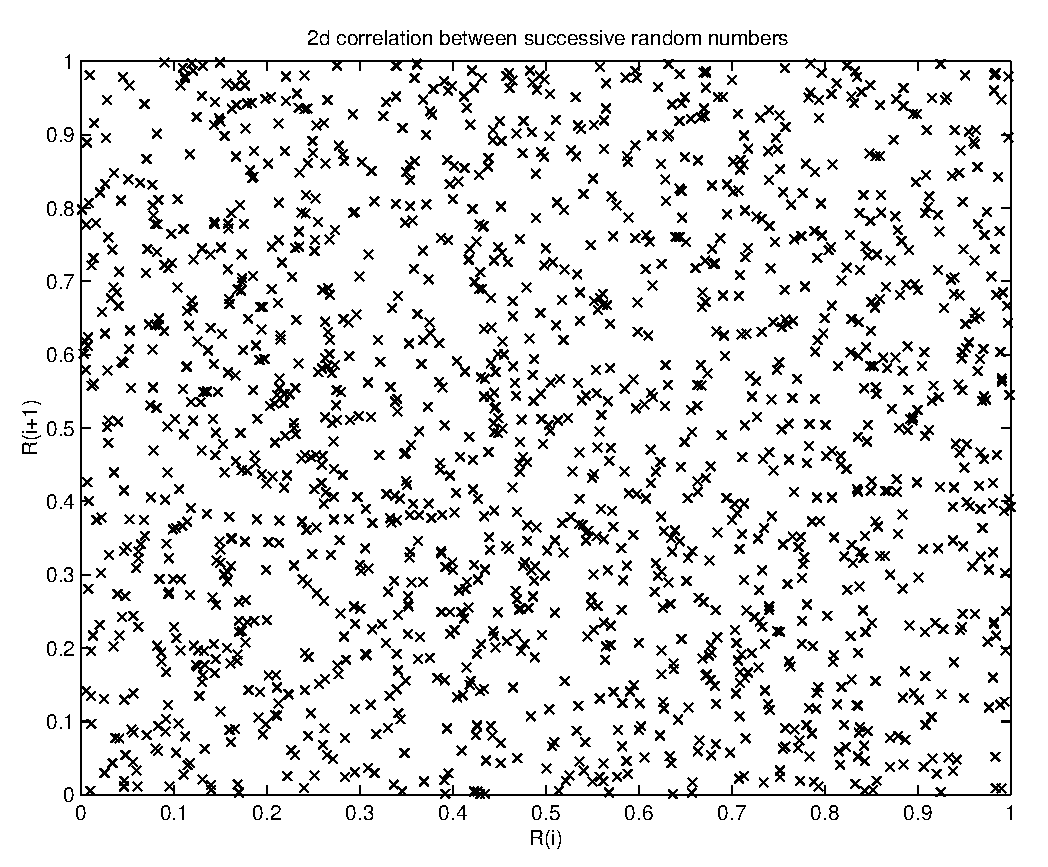
\includegraphics[width=10cm]{./Figures/f_trandom2_3.eps}
\caption{Correlation between successive values in a series of 3000 
random numbers generated for $a=65539$, $c=0$, $M=2^{31}-1$.}
\end{figure}


\begin{figure}
\label{F_TRANDOM2_4}
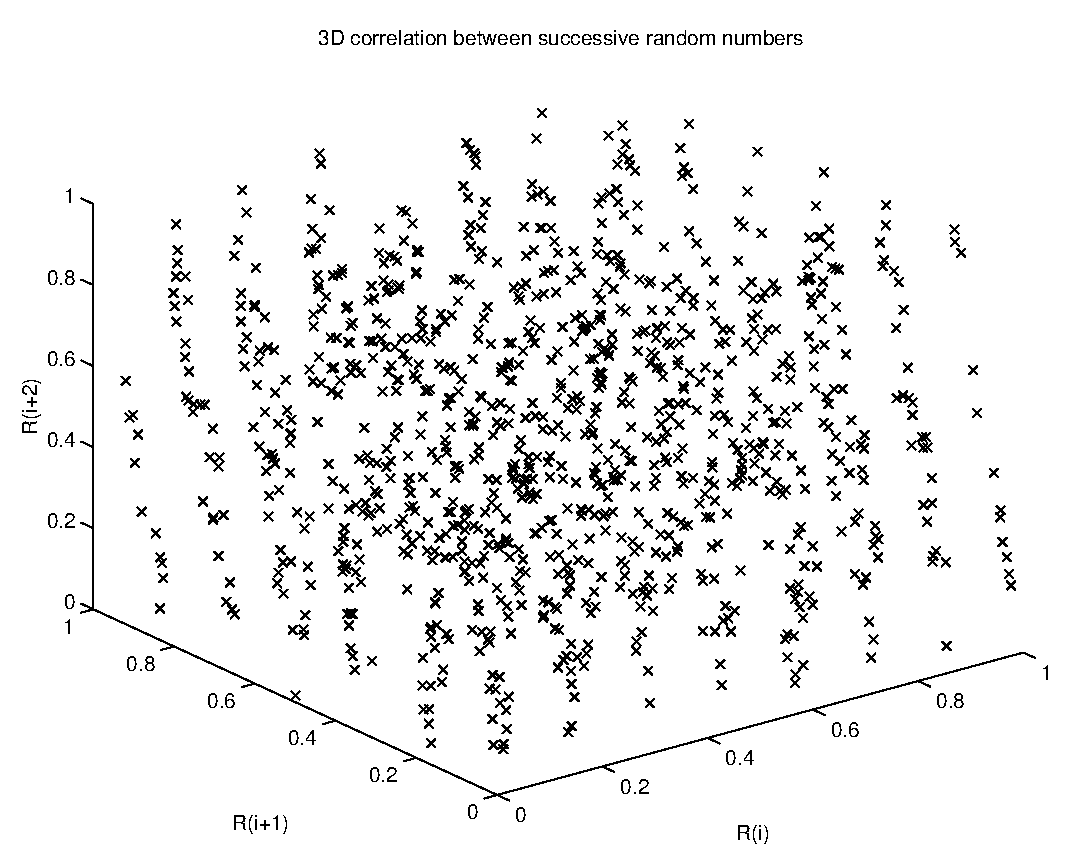
\includegraphics[width=10cm]{./Figures/f_trandom2_4.eps}
\caption{Correlation between successive values 
$R(i),R(i+1), R(i+2)$ in a series of 3000 random numbers generated
for $a=65539, c=0, M=2^{31}-1$.}
\end{figure}

The figures clearly reveal that the generator is not perfect.
In the exercise we will learn that choosing $a=16807$, the minimal
standard generator, 
significantly improves the performance. The performance of 
this minimal standard generator can be increased by shuffling
the output to remove low--order serial correlations (EXERCISE!!!!)
({\sf ran1} of Numerical Recipes).

In the book by Press et al. other "Quick and Dirty" linear 
congruential generators
are presented. Furthemore, serial correlations can be broken up by 
combining two linear congruential generators.

There are also other algorithms for the generation of random 
numbers: Shift--register generators (Lit: Kirkpatrick and Stoll), 
Fibonacci generators (lit: Knuth, James) or quasi--random numbers 
and we refer the reader to the original literature.

\section{The Transfomation method: Invertible distributions}
In the previous section we have learned how to generate random 
numbers with a uniform probability distribution, so that the 
probability $p(x)dx$ to generate a random number between $x$ and $x+dx$
is given by
\begin{equation*}
P(x)dx = \left\{ \begin{array}{ll}
                   dx & 0<x<1 \\
                   0   & {\rm otherwise}.
                  \end{array}
         \right.
\end{equation*}
With the help of the random variable transformation theorem it is easy
to transform uniform deviates into random numbers which are 
distributed according to invertible, one--to--one, distributions.
We know from Chap. 2 that if we take a uniform deviate $x$ and then 
transform it to a new variable $y(x)$ the probability distribtion
of $y$ is given by
\begin{equation}
p(y) = p(x) \left| \frac{dx}{dx}\right|.
\end{equation}
We want to derive a transformation which generates random numbers 
which are distributed according to a given
$p(y)$. Since $x$ is uniformly distributed the 
above equation reduces to
\begin{equation}
\label{INVERTIBLE}
\frac{dx}{dy} = p(y),
\end{equation}
which can be easily integrated
\begin{equation*}
x(y) = P(y) = \int^y p(y')dy'.
\end{equation*}
Hence, the transformation we are looking for is given by the 
inverse of $P(y)$. Thus, a random variable $Y$ with density $p(y)$
can be generated by uniform deviates trough
\begin{equation*}
Y = Y(X) = P^{-1}(X).
\end{equation*}
In the following we will apply this method to generate 
exponentially and gaussian distributed random numbers.

\subsection{Exponential distribution}
Let $p(y)= w\exp(-wy)$ for positive $y$. It follows from Eq. (\ref{INVERTIBLE})
that
\begin{equation*}
\frac{dx}{dy} = w \exp(-wy).
\end{equation*}
Therefore we get immediately
\begin{equation*}
x(y) = \int_0^{\infty} dy'w\exp(-wy') = 1-\exp(-wy).
\end{equation*}
The above expression is easily inverted
\begin{equation*}
y=-\frac{1}{w}\ln(1-x),
\end{equation*}
and since $x$ is equally distributed in $[0,1]$ we can generate 
exponentially distributed random numbers with the help of the 
formula
\begin{equation}
y = - \frac{1}{w} \ln(x).
\end{equation}
It is clear that in MATLAB such an exponentially distributed 
random number $Y$ can be generated with the help of the following 
line of code
\begin{verbatim}
y = - log( rand(1) )/w
\end{verbatim}
With the help of the simple program {\sf expdistr} we want to 
generate 1000 exponentially distributed random numbers and compare
them with the prescribed distribution. We check also the mean 
value and variance and compare them with the analytical expectation 
values.

\subsubsection{Listing of the program expdistr.m}

In Fig. (\ref{F_EXPDISTR}) we see the histogram of 1000 drawn exponentially 
distributed random numbers.
\begin{figure}
\label{F_EXPDISTR}
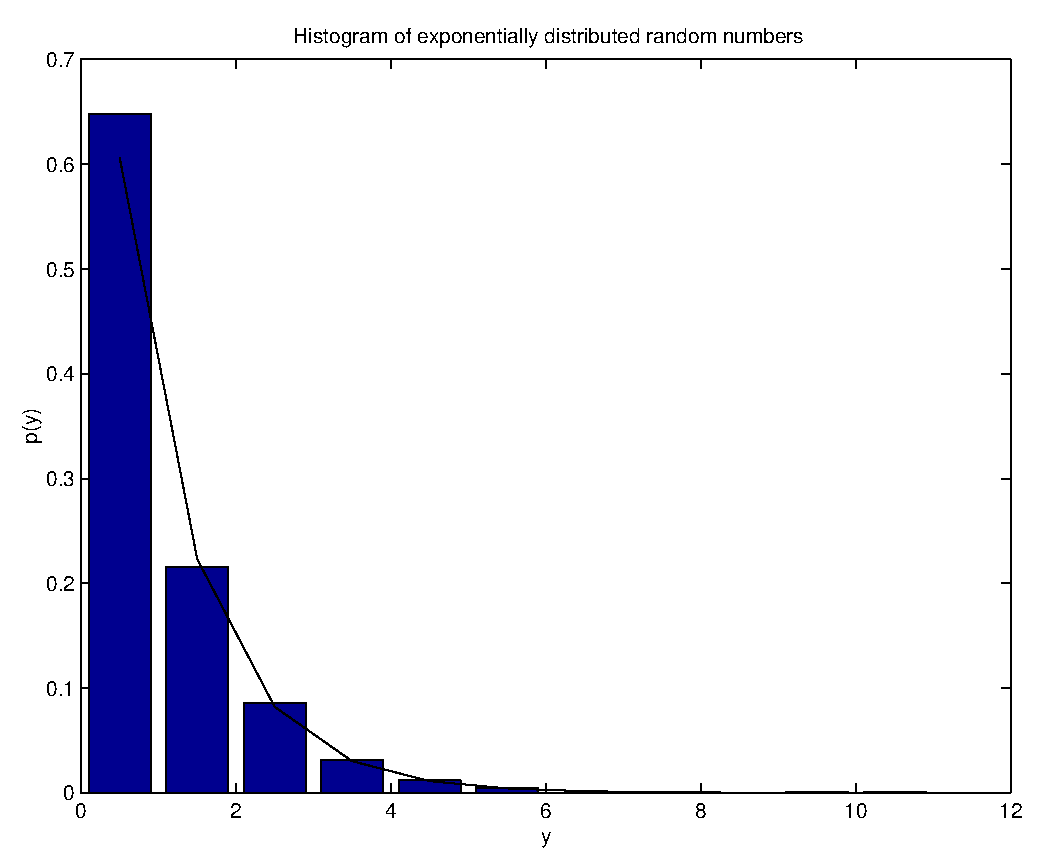
\includegraphics[width=10cm]{./Figures/f_expdistr.eps}
\caption{Histogram of 1000 exponentially distributed random numbers with
mean 1 generated according to the transformation method. The continuous
line represents the expected exponential distribution.}
\end{figure}

\subsection{Gaussian distributed random numbers}
Gaussian distributed random numbers can be obtained with the help 
of the multidimensional random variable transformation theorem.
Let us consider the transformation
\begin{eqnarray}
\label{GAUSS-GEN1}
y_1 & = & \sqrt{-2\log(x_1)} \cos(2 \pi x_2) \\
\label{GAUSS_GEN2}
y_2 & = & \sqrt{-2\log(x_1)} \sin(2 \pi x_2),
\end{eqnarray}
where $X_1$ and $X_2$ are uniformly distributed random numbers on 
the interval $[0,1)$. Equivalently we can write
\begin{eqnarray*}
x_1 & = & \exp[-\frac{1}{2}(y_1^2+y_2^2)] \\
x_2 & = & \frac{1}{2 \pi} \arctan\left( \frac{y_1}{y_2}\right).
\end{eqnarray*}
it is now straightforward  to show that the Jacobian determinant
reads
\begin{equation*}
\frac{\partial(x_1,x_2)}{\partial(y_1,y_2)} = 
   - \left[ \frac{1}{\sqrt{2 \pi}} \exp(-y_1^2/2)\right]
   \left[ \frac{1}{\sqrt{2 \pi}} \exp(-y_2^2/2)\right].
\end{equation*}
The right hand side of the above equation corresponds to the 
product of two independent Gaussian distributions. Thus it follows
from the multidimensional version of the random variable 
transformation  theorem for invertible distributions that the
two random number generated according to Eqs. (\ref{GAUSS-GEN1}) 
and (\ref{GAUSS-GEN2}) are Gaussian distributed. This algorithm 
which allows the generation of two Gaussian random numbers from 
two uniformly distributed ones is called the Box--Muller method.

It is clear that it easy to implement the above algorithm in 
MATLAB. This is done in the program {\sf gaussdistr.m} which generates
gaussian random numbers with mean value $mu$ and variance $sigma$.

\subsubsection{Listing of the program gaussdistr.m}

The corresponding histogram obtained by running the program for
n=1000, mu=0, sigma=2 can be seen in Fig. (\ref{F_GAUSSDISTR}).
\begin{figure}
\label{F_GAUSSDISTR}
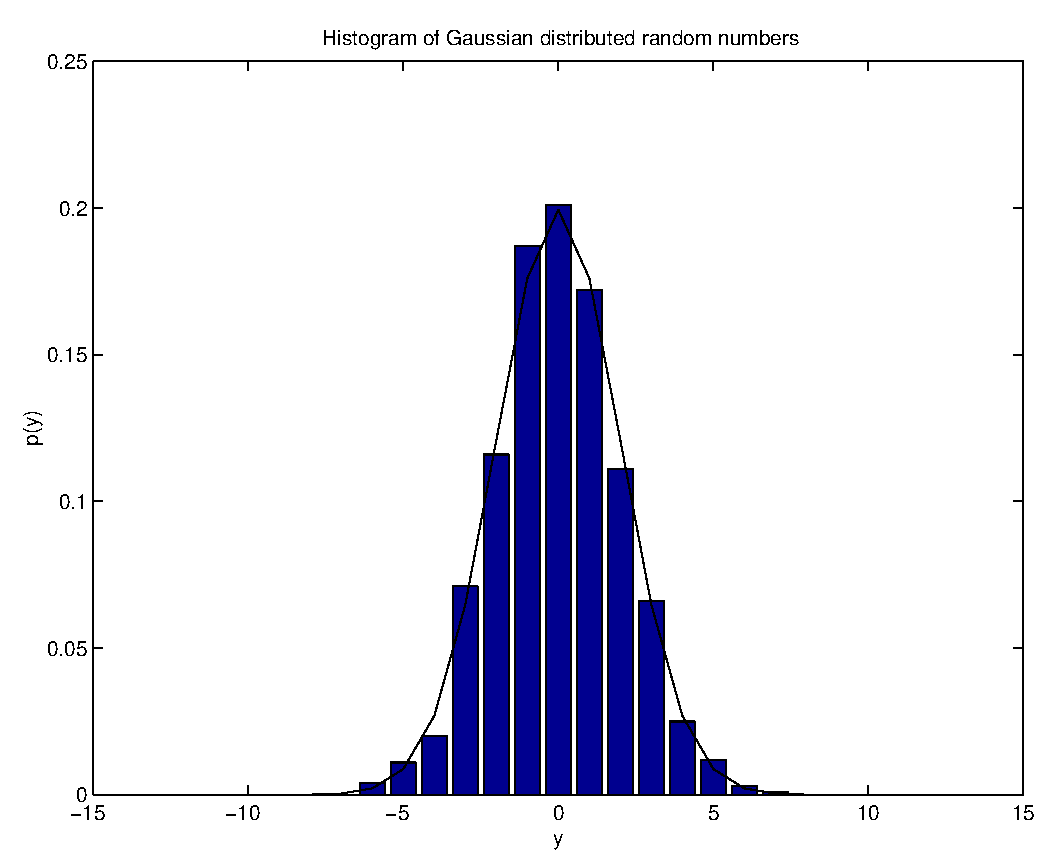
\includegraphics[width=10cm]{./Figures/f_gaussdistr.eps}
\caption{Histogram of 1000 Gaussian distributed random numbers with
mean 0 and variance 2 generated according to the Box-Muller method. 
The continuous line represents the expected Gaussian density.}
\end{figure}

Let us end this subsection by mentioned that normal distributed
random numbers can be generated in MATLAB with the help of 
the function {\sf randn}.

\section{The acceptance--rejection technique}
The acceptance--rejection technique is a method of wide 
applicability. In its original formulation it is due to 
von--Neumann. The basic idea is to sample a random number
from some known and appropriate probability distribution and to 
perform a test to determine whether or not it is acceptable for 
use or not. We follow Rubinstein but consider for simplicity only
the one--dimensional case.

Let us assume that the stochastic variable $X$ is defined on the 
interval $a \le x \le b$ and is distributed according to the
probability density $p(x)$. We write this probability distribution 
as
\begin{equation*}
p(x) = C d(x) q(x),
\end{equation*}
where $C$ is a normalization constant $C \ge 1$, $q(x)$ is also a 
probability distribution and $0 \le d(x) \le 1$. The probability 
distribution $q(x)$ is the importance function, and  we are 
supposed to know how to generate random variates distrubuted 
according to it.

The accepatnce--rejection method works as follows. We generate two
random variates, $\xi$ is uniformly distributed on the interval
$[0,1)$ and $Y$ is distributed according to $q(y)$. Then we test
whether or nor the equality
\begin{equation*}
\xi \le d(y)
\end{equation*}
holds or not. If  the conditione $\xi \le d(y)$ is satisfied, 
then $Y$ is accepted as 
a random variate distributed according to $p(x)$.  If
the condition is not satisfied, the pair $(\xi,y)$ is rejected, 
and we have to try again.

It is easy to demonstrate that the above methd works. Let us apply
Bayes'formula to the conditional probability $p(x|\xi \le d(y)$:
\begin{equation}
\label{A-R-BAYES}
p(x|\xi \le d(y) = \frac{{\rm Prob}(p(x|\xi \le d(y)|Y=x)q(x)}
                  {{\rm Prob}(\xi \le d(y))}.
\end{equation}
It is straightforward to compute
\begin{eqnarray*}
{\rm Prob}(p(x|\xi \le d(y)|Y=x) &=& {\rm Prob}(\xi \le d(x)) = 
          d(x) \\
{\rm Prob}(\xi \le d(y)) & = & \int {\rm Prob}(\xi \le d(Y|Y=x)) q(x) dx \\
               &= & \int q(x) d(x)dx = \int dx \frac{p(x)}{C} = 
                   \frac{1}{C}.
\end{eqnarray*}
Inserting into (\ref{A-R-BAYES}) we obatin finally
\begin{equation*}
p(x|\xi \le d(y) = p(x),
\end{equation*}
which completes the proof.

The above discussion also makes evident the role of the constant
$C$. The efficiency of the method depends on the inequality $\xi \le 
d(y)$, for independent trials the probability of success is given 
by $1/C$. $C$ represents the average number of passes which must 
be made with the algorithm in order to select a variate. It is 
clear, that in order for the method to be efficient it must be 
easy to generate random numbers according to $q(x)$ and the 
efficiency should be large, i.e., $C$ should be close to one.

In the original formulation by von--Neumann the comparison 
function was simply chosen to be the uniform distribution. If
$M$ is the maximum of $p(x)$ then we choose
\begin{eqnarray*}
q(x) & = & \frac{1}{b-a} \\
d(x) & = & \frac{p(x)}{M} \\
C & = & M(b-a).
\end{eqnarray*}
The von--Neumann algorithm then simply reads \\
1. Generate $\chi_1$ and $\chi_2$ uniformly distributed in 
    $[0,1)$. \\
2. Evaluate $Y=a+\chi_2(b-a)$. \\
3. If $\chi_1 \le p(x)/M$ then $Y$ is a variate distributed 
    according to $p(x)$. \\
4. Go to 1.

As a simple example we want to generate random numbers on $[0,1)$    
distributed according to
\begin{equation*}
p(x) = 3x^2; \;\;\; 0 \le x <1.
\end{equation*}
We choose $C=3$ and apply the von--Neumann algorithm. \\
1. Generate $\chi_1$ and $\chi_2$ uniformly distributed in 
    $[0,1)$. \\
2. Test the inequality $\chi_1 \le \chi_2^2.$     \\
3. If the equality holds we accept $\chi_2$ as a random number 
generated according to $p(x)$.

The above algorithm has been implemented in MATLAB in the program
{\sf neumann.m}, which we run for $n=1000$ and $n=5000$. The 
result of the latter run can be seen in Fig. (\ref{F_NEUMANN}).
\begin{figure}
\label{F_NEUMANN}
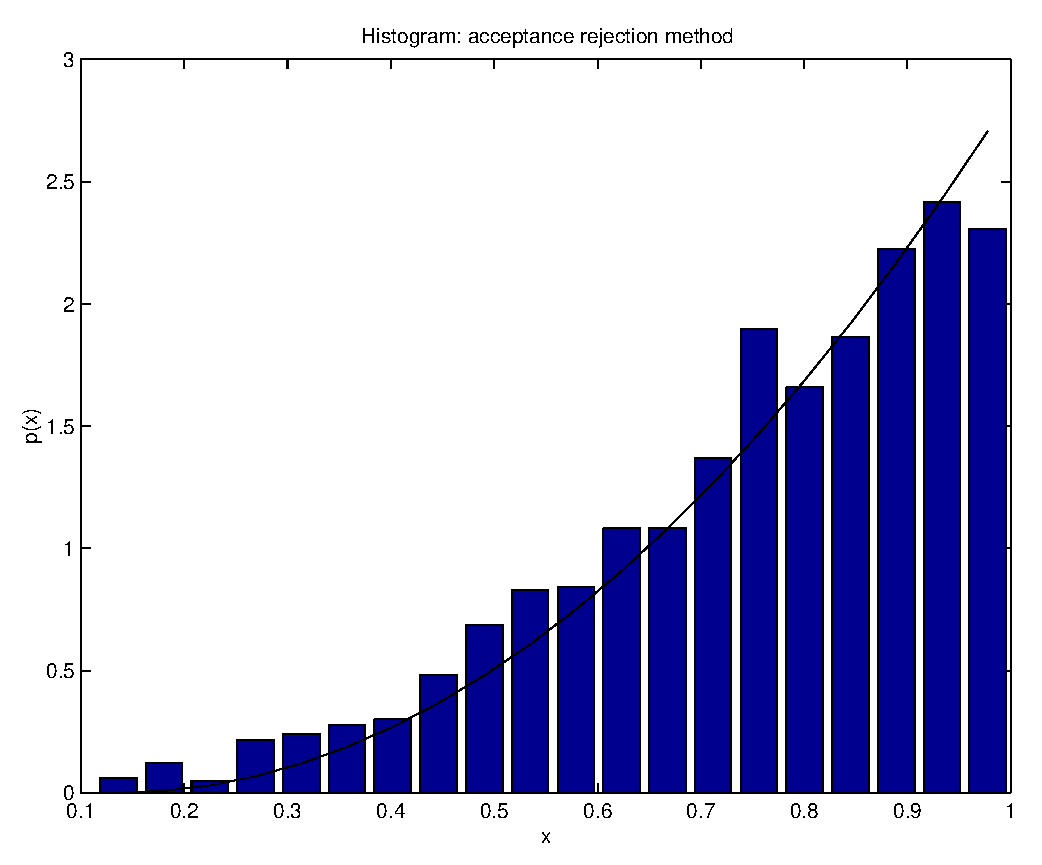
\includegraphics[width=10cm]{./Figures/f_neumann.eps}
\caption{Histogram of 5000 random numbers distributed
according to $p(x) = 3x^2$ generated with the von--Neumann
acceptance--rejection technique.
The continuous line represents the exact density $p(x)$.}
\end{figure}
In the program we count the number of successful trials. The ratio
of successful trials to the total number of drawn random pairs for 
the run shown
is 0.3328, which is in good agreement we the expected theoretical
value of $1/C=1/3$.

\subsubsection{Listing of the program neumann.m}




%\subsection{Poisson distributed random numbers}

\section{Variance reduction: Importance Sampling}
In this section we will see how the Monte--Carlo integration
algorithms can considerably be improved. The importance sampling 
technique will be our first encounter with a so--called variance 
reduction technique. We already know that the estimation of 
integrals by the Monte--Carlo method is affected with errors. The
basic idea of variance reduction techniques is to use known 
informations about the problem in order to improve the efficiency 
of the simulation. Obviuosly, if nothing is known about the 
problem no variance reduction can be achieved. On the other 
extreme, if we have full knowledge the variance will be reduced to 
zero, and there will be no need for a simulation. It is always 
important to be aware of what is known about the system.

We now consider the problem of estimating the integral
\begin{equation}
\label{INT_VARRED}
I = \int dx f(x).
\end{equation}
The central idea of importance sampling is to select random 
variates from regions in proportion to the importance these 
regions make to the integral we want to evaluate, instead of 
spreading them evenly. To this end we rewite the integral 
(\ref{INT_VARRED}) in the form
\begin{equation*}
I = \int \frac{f(x)}{p(x)} p(x) dx = \langle 
\frac{f(x)}{p(x)}\rangle,
\end{equation*}
where $X$ is a random variable with probability density $p(x)$.
$P(x)$ is called the importance sampling distribution.  Since the
integral is obviously the expectation value of the function $f(x)/p(x)$
it can be estimated using $N$ random numbers $X_i$ distributed 
according to $p(x)$
\begin{equation*}
\hat{I}_N = \frac{1}{N} \sum_{i=1}^N \frac{f(x_i)}{p(x_i)}.
\end{equation*}
The function $p(x)$ has to be chosen in such a way that the 
variance of $f(x)/p(x)$ 
\begin{equation*}
{\rm Var} = \langle (\frac{f(x)}{p(x)}-I)^2\rangle
   = \int_a^b \frac{f^2(x)}{p(x)}dx - I^2
\end{equation*}
is minimal. If $f(x)>0$ it follows from the above equation that
${\rm Var}=0$ if we choose $p(x)$ as $p(x) = f(x)/I$. 
Unfortunately, this choice implies that we have to know already 
the integral we want to solve. In general, the variance can 
essentially be reduced if $p(x)$ is chosen to resemble $f(x)$.

As an example we consider the integral
\begin{equation}
\label{I_MCI_IS}
I= \int_0^1 dx \exp(-x^2).
\end{equation}
In the first two columns of table (\ref{T_MCI_IS}) we show
the results of two estimates of the above integral with the 
help of the standard Monte--Carlo integration. In the third column 
we show the results of the importance sampling integration.

\begin{table}\label{T_MCI_IS}
\caption{Monte--Carlo estimates of the integral (\ref{I_MCI_IS})
using the standard method $p(x)=1$ and the importance sampling method
$p(x)=a\exp(-x)$}
\begin{center}
\begin{tabular}{llll}
 ~             & $p(x) =1$ & $p(x) =1$ & $p(x)=a\exp(-x)$ \\ \hline
$N$            & 1000      & 16384      & 1000           \\
$I$            & 0.736087  & 0.74504    & 0.748340        \\
$\sigma_I$     & 0.00131   & 0.000317   & $9.65 \times 10^{-5}$ \\
CPU time/trial (s) & 0.000660  & 0.003837   & 0.000860  \\
total CPU time (s) & 0.66      & 62.86      & 0.86 
\end{tabular}
\end{center}
\end{table}
The simulation was performed with the help of the program
{\sf mciis.m} whose listing can be seen below.

\subsubsection{Listing of the program mciis.m}
%\includelistings{.\Listings\mciis.m}

The importance sampling function is chosen to be $p(x)=a\exp(-x)$,
where the constant $a$ is chosen such that $p(x)$ is normalized
on the  unit interval. Accordingly the $N$ random numbers $X_i$
distributed according to $p(x)$ are generated with the help of the
inversion method. Since
\begin{equation*}
P(x) = \int_0^x dx' p(x') = a[1-\exp(-1)]
\end{equation*}
the exponentially distributed random numbers on the interval $[0,1)$
are generated according to
\begin{equation*}
X = - \log(1- \chi/a),
\end{equation*}
where the $chi$ are uniformly distributed random numbers on the 
interval $[0,1)$. The generation of these random numbers is 
performed in lines x to y.

It is important to remark that although the computation time per
trial is larger in the importance sampling technique the total CPU 
time is smaller compared to the standard Monte Carlo algorithm 
because a much smaller number of realizations is required in order
to achieve a desired accuracy (variance).





\section{Self--Avoiding random walks}
\subsection{Simple sampling}
\subsection{Importance sampling}
%%%%%%%%%%%%%%%%%%%%%%%%%%%%%%%%%%%%%%%%%%%%%%%%%%%%
%%%%%%%%%%%%%%%%%%%%%%%%%%%%%%%%%%%%%%%%%%%%%%%%%%%%%
%%%%%%%%%%%%%%%%%%%%%%%%%%%%%%%%%%%%%%%%%%%%%%%%%%%%%
%%%%%%%%%%%%%%%%%%%%%%%%%%%%%%%%%%%%%%%%%%%%%%%%%%%%%
%%%%%%%%%%%%%%%%%%%%%%%%%%%%%%%%%%%%%%%%%%%%%%%%%%%%%
%%%%%%%%%%%%%%%%%%%%%%%%%%%%%%%%%%%%%%%%%%%%%%%%%%%%%
%%%%%%%%%%%%%%%%%%%%%%%%%%%%%%%%%%%%%%%%%%%%%%%%%%%%%
\chapter{Stochastische Prozesse}
Master-Gleichungen

\chapter{Monte Carlo Methoden in der statistischen Mechanik}
Metropolis; Ising; Finite-Size Effects; Random Walks; SAW (?)
Simulated annealing; travelling salesman;

\chapter{Non-equilibrium MC}
Chemische Reaktionen, Diffusion; Reaktions-Diffusion, Turbulenz.

\chapter{Brownsche Dynamik Simulationen}
Omega-entwicklung; SDE;


\chapter{Rest}
stochastische Resonanzen; Muster Erkennung; random Walks;

\chapter{Stochastische Wellenfunktionsmethoden}


%%% Chapter 4 
\chapter{Markov processes and master equations}
This chapter is devoted
to the introduction of some mathematical concepts, which allow the
correct treatment of time--dependent probabilistic phenomena. 
Such processes occur in many branches of physics. A typical example,
is for instance, the dynamics of the velocity field in a turbulent fluid.
We will introduce stochastic processes as time dependent stochastic 
variables and we will 
learn how the dynamics of a particular class of stochastic 
processes, the so--called Markov processes  is described 
with the help of differential Chapman--Kolmogorov equations. 
These concepts will be applied
in the next chapters to typical examples from statistical physics.

\section{Stochastic processes}
We have already learned in Chap. 2 that once a stochastic variable 
$X$ has been defined it is possible to define other stochastic 
variables, say $Y$, as functions of $X$ by some mapping $f$. In 
particular, the quantity $Y$ may be a function of an additional
time variable $t$, i.e.,
\begin{equation*}
Y(t) = f(X,t).
\end{equation*}
Sloppy speaking, such a quantity $Y(t)$ is called a {\em stochastic
processes}. If we insert for $X$ one of its possible values $x$
we obtain an ordinary function
\begin{equation*}
y(t) = f(x,t),
\end{equation*}
which is a {\em realization} of the stochastic process
\cite{VAN_KAMPEN}. It is 
customary in statistical physics to regard the stochastic process 
as an {\em ensemble} of such realizations.

It follows immediately from the random variable transformation 
theorem that the probability density for $Y(t)$ to take the value
$y$ at time $t$ is given by
\begin{equation*}
P_1(y,t) = \int dx  \delta(y-f(x,t)) P(x)
\end{equation*}
and, accordingly, the joint probability density that $Y$ has the
value $y_1$ at time $t_1$, the value $y_2$ at time $t_2$, 
$\ldots$, and the value $y_n$ at time $t_n$ is given by
\begin{eqnarray*}
\lefteqn{P_n(y_1,t_1;y_2,t_2; \ldots, y_n,t_n)} \\
&& = \int dx \delta(y_1-f(x,t_1))\delta(y_2-f(x,t_2)) \cdots 
   \delta(y_n-f(x,t_n))  P(x).
\end{eqnarray*}
In such a way an infinite hierarchy of joint probability densities
$P_n$ $(n=1,2,\ldots)$ is defined, which allows the evaluation of 
expectation values like
\begin{eqnarray*}
\lefteqn{<Y(t_1) Y(t_2) \cdots Y(t_n)>} \\
&& = \int dy_1 \int dy_2 \cdots \int dy_n 
        y_1 y_2 \cdots y_n P_n(y_1,t_1;y_2,t_2; \ldots, y_n,t_n).
\end{eqnarray*}
It has been shown by Kolmogorov (\cite{VAN_KAMPEN}) that the 
hierarchy of joint probability densities introduced above 
completely specifies
a stochastic process if the following four consistency conditions 
are satisfied \\
(i) $P_n \ge 0$; \\
(ii) $P_n$ is a symmetric function of the pairs $(y_1,t_1)$, 
$\ldots$, $(y_n,t_n)$; \\
(iii) $\int dy_n P_n(y_1,t_1; \ldots , y_n,t_n) =
     P_{n-1}(y_1,t_1; \ldots ; y_{n-1},t_{n-1})$; \\
(iv) $\int dy_1 P(y_1,t_1) =1$.

Thus, the hierarchy of joint probability densities constitutes an 
alternative way to define stochastic processes. 
With increasing $n$ the description of the stochastic process gets
more precise. It is important to 
make the following remarks.  The condition (iii) implies that each 
density $P_n$ includes the knowledge of all previous densities
$P_k$ with $k<n$. Furthermore, the density $P_n$ does have the 
following property if two time arguments are identical
\begin{equation*}
P_n(x,t;y_1,t;y_2,t_2; \ldots ; y_{n-1},t_{n-1}) = 
P_{n-1}(x,t;y_2,t_2; \ldots ; y_{n-1},t_{n-1})
\delta(x-y_1).
\end{equation*}
The hierarchy of probability densities is also the starting point 
for the classification of stochastic processes. A stochastic 
process is said to be purely random if events at different times 
are not correlated. In this case the joint probability density 
factorizes, i.e. we have
\begin{eqnarray*}
P_2(y_1,t_1;y_2,t_2) &=& P_1(y_1,t_1) P_1(y_2,t_2) \\
P_3(y_1,t_1;y_2,t_2;y_3,t_3) &=& P_1(y_1,t_1) P_1(y_2,t_2)P_1(y_3,t_3) 
\\
\text{and so on.} &&
\end{eqnarray*}
This means that the value of $Y$ at time $t$ is completely 
independent of its values in the past and in the future. An even
more special case occurs when the $P_1(y_i,t_i)$ are independent 
of $t_i$. In this case the same probability law governs the 
process for all times. Such processes are called
{\em Bernoulli trials} (\cite{gardiner}). In the next section we 
will introduce the next most simple class, the {\em Markov processes},
in which the knowledge of only the presents determines the future.


\section{Markov processes}
In order to define the class of stochastic processes, which will be 
of central importance in the forthcoming theoretical discussions 
and in the examples of the next chapters, we will formulate
the {\em Markov assumption}. This assumption is formulated in 
terms of conditional probability densities which we 
will denote by
$T_n(x,t|y_1,t_1;y_2,t_2; \ldots, y_n,t_n)$. This quantity gives 
the probability that the stochastic process takes the value $x$ at 
time $t$ given that it had the value $y_1$ at time $t_1$, $y_2$
at time $t_2$, $\ldots$, $y_n$ at time $t_n$, where we assume that
$t_1< \cdots <t_n < t$.  The conditional probability density has 
the following properties \\
(i) $T_n \ge 0$, \\
(ii) $\int dx T_n = 1$,  \\
(iii) $T_n(x,t|y_1,t;y_2,t_2; \ldots, y_n,t_n) = \delta(x-y_1)$.\\
As we already know the joint probability density $P_n$ can be 
expressed with the help of Bayes' theorem through the conditional 
probability density $T_{n-1}$ as
\begin{eqnarray*}
\lefteqn{P_n(x,t;y_1,t_1;y_2,t_2; \ldots, y_{n-1},t_{n-1})} \\
&& = P_{n-1}(y_1,t_1;y_2,t_2; \ldots, y_{n-1},t_{n-1})
T_{n-1}(x,t|y_1,t_1;y_2,t_2; \ldots, y_{n-1},t_{n-1}).
\end{eqnarray*}
Now we are in the position to define the class of Markov 
processes. Let $t_1< \cdots <t_n < t_{n+1}$ be an ordered sequence 
of times. A Markov process is defined through the following 
condition for the conditional probability density of the
stochastic process
\begin{equation*}
T_{n}(y_{n+1},t_{n+1}|y_1,t;y_2,t_2; \ldots, y_{n},t_{n})
= T_{1}(y_{n+1},t_{n+1}|y_{n},t_{n}).
\end{equation*}
In other words, the conditional probability density at $t_{n+1}$
given the value of $y_n$ at time $t_n$ is uniquely determined and 
is not affected by any value of $y$ at earlier times. Thus, the
conditional probability density is determined completely by the 
knowledge of the most recent condition.
The above definition implies that for a Markov process all
$T_n$ with $n \ge 1$ can be determined from the
conditional probability density $T_1$, which will also be called
the one step 
transition probability density. As an immediate consequence a Markov 
processes is completely characterized by the knowledge of the
one step transition probability and by the probability density
$P_1$. With the help of these two functions we can reconstruct the 
whole hierarchy of probability densities. For example, we
have
\begin{eqnarray}
\label{P3}
P_3(y_1,t_1;y_2,t_2;y_3,t_3) &=& 
      P_2(y_1,t_1;y_2,t_2) T_2(y_3,t_3|y_1,t_1;y_2,t_2)   
         \nonumber \\
    & = & T_1(y_3,t_3|y_2,t_2) T_1(y_2,t_2|y_1,t_1)
           P_1(y_1,t_1).
\end{eqnarray}
Integrating the above equation (\ref{P3}) over $y_2$ we obtain 
\begin{equation}
P_2(y_1,t_1;y_3,t_3) = P_1(y_1,t_1) 
       \int dy_2 T_1(y_3,t_3|y_2,t_2) T_1(y_2,t_2|y_1,t_1).
\end{equation}
Dividing both sides by $P_1(y_1,t_1)$ we obtain an identity which 
must be obeyed by the transition probability of any Markov process
\begin{equation}
\label{CHAPMAN_KOLMOGOROV}
T_1(y_3,t_3|y_1,t_1) =  
       \int dy_2 T_1(y_3,t_3|y_2,t_2) T_1(y_2,t_2|y_1,t_1).
\end{equation}
The above identity is called the {\em Chapman--Komogorov 
equation}. It has a simple interpretation. The transition 
probability between two states $y_1$ and $y_3$ with $t_1 <t_3$
corresponds to the product of the transition probability between 
the initial state and some intermediate state and the transition 
between this intermediate state and the final state integrated
over all intermediate states.

As we already noted the functions $P_1$ and $T_1$ uniquely define 
a Markov process. However, these two functions are not arbitrary.
They must satisfy the Chapman--Kolmogorov equation and the obvious
consistency condition
\begin{equation}
\label{CONSISTENCY}
P_1(y_2,t_2) =  
       \int dy_1  T_1(y_2,t_2|y_1,t_1) P_1(y_1,t_1).
\end{equation}
For the sake of a compact notation we will write now $P=P_1$ and 
$T=T_1$.


\section{The differential Chapman--Kolmogorov equation}
We now derive a differential  form of the Chapman--Kolmogorov 
equation which is more practical for physical applications.
We will proceed in two steps. First, we introduce the concept
of generator of a stochastic process. Second, we will construct
with the help of the generator an equation of motion for the
transition probabilty density.

\subsection{The generator of a Markov process}
We consider the time evolution of the expectation value
of  a function $f(y)$.
Thus,
\begin{eqnarray*}
\frac{\partial}{\partial t} \langle f(y) \rangle &=&
 \frac{\partial}{\partial t} 
    \left\{  \int dy f(y) P(y,t)  \right\}  \\
 &= & \lim_{\Delta t \rightarrow 0} \frac{1}{\Delta t}
       \left\{  \int dy f(y) \left[P(y,t+\Delta t) - P(y,t) \right]  
       \right\}.
\end{eqnarray*}
Making use of the consistency condition (\ref{CONSISTENCY}) 
in the first term 
on the right--hand side of the above equation we obtain
\begin{equation*}
\frac{\partial}{\partial t} \langle f(y) \rangle =
   \lim_{\Delta t \rightarrow 0} \frac{1}{\Delta t}
    \left\{  \int dy \int dy' f(y) T(y,t+\Delta t|y',t) P(y',t) 
         - \int dy f(y) P(y,t) 
       \right\}.
\end{equation*}
We rename the integration variables in the positive 
term of the right--hand side of the above equation ($y \rightarrow y'$,
$y' \rightarrow y$) to obtain
\begin{equation*}
\frac{\partial}{\partial t} \langle f(y) \rangle =
   \lim_{\Delta t \rightarrow 0} \frac{1}{\Delta t}
    \left\{  \int dy  \int dy' \left[ f(y') T(y',t+\Delta t|y,t) 
         - \delta(y-y') f(y') \right] P(y,t) 
       \right\},
\end{equation*}
which we can also write as
\begin{equation*}
\frac{\partial}{\partial t} \langle f(y) \rangle =
\int dy P(y,t) \lim_{\Delta t \rightarrow 0} \frac{1}{\Delta t}
\left\{ \int dy' \left[ f(y') T(y',t+\Delta t|y,t) 
         - \delta(y-y') f(y') \right].
\right\}
\end{equation*}
At this point it is convenient to introduce the infinitesimal 
generator of a Markov process ${\cal{A}}$ as
\begin{equation}
\label{DEF_GENERATOR}
{\cal{A}}(t) f(x) = \lim_{\Delta t \rightarrow 0}
    \frac{1}{\Delta t} 
    \left[\int dy f(y)T(y,t+\Delta t|x,t) - f(x)  \right].
\end{equation}
$f(y)$ is some measurable function for which the above 
limit exists. Evidently ${\cal{A}}$ is a linear operator, which 
can be determined from the transition probability density. 
When the operator ${\cal{A}}$ operates on $f$ it describes the
change of the expectation value of $f$ in an infinitesimal time 
step. As a consequence of the Chapman--Kolmogorov equation each time 
step $t-t_1$ can be decomposed into a sequence of smaller time 
steps. So it is plausible to characterize the Markov
process by regarding infinitesimal time steps. 
The importance of the generator ${\cal{A}}$ lies in the fact
that together with some initial condition $P(x,t=0)$ it specifies
uniquely the Markov process.
The time evolution equation for the expectation value can be written 
in the compact and suggestive form
\begin{equation}
\label{EQ_EXPECTATION}
\frac{\partial}{\partial t} \langle f \rangle = 
\langle {\cal{A}} f \rangle.
\end{equation}


\subsection{The differential Chapman--Kolmogorov equation}
With the help of the generator we derive an equation of motion for
the transition probability $T$.
Multiplying equation (\ref{DEF_GENERATOR}) 
with $T(x,t|x',t')$ ($t'<t$) and 
integrating over $x$ we obtain
\begin{eqnarray*}
\lefteqn{\int dx \left[ {\cal{A}}(t) f(x) \right] T(x,t|x',t')} \\
&& = \lim_{\Delta t \rightarrow 0}
    \frac{1}{\Delta t} 
    \left[\int dy f(y)T(y,t+\Delta t|x',t') - 
        \int dx f(x) T(x,t|x',t')  \right],
\end{eqnarray*}
where we made use of the Chapman--Kolmogorov equation.
We now rename the variable $y$ on the right--hand side of the above 
equation and call it $x$ and perform the limit $\Delta t \rightarrow 
0$
\begin{equation}
\label{KOL_FORWARD_0}
\int dx \left[ {\cal{A}}(t) f(x) \right] T(x,t|x',t') =
  \int dx f(x) \frac{\partial}{\partial t} T(x,t|x',t').
\end{equation}
It is convenient to introduce the adjoint operator ${\cal{A}}^{\dagger}$
to the generator ${\cal{A}}$ according to the following definition
\begin{equation}
\label{ADJOINT}
\int dx \left[ {\cal{A}}(t) f(x) \right] T(x,t|x',t') \equiv
\int dx f(x) \left[ {\cal{A}}^{\dagger}(t)  T(x,t|x',t') \right].
\end{equation}
We will see in the next sections how the adjoint operator is
explicitely constructed.
Inserting Eq. (\ref{ADJOINT}) into Eq. (\ref{KOL_FORWARD_0})
and considering that (\ref{ADJOINT}) holds for any 
function $f(x)$ we conclude that the equation of motion for the 
transition probability is given by
\begin{equation}
\label{KOL_FORWARD}
\frac{\partial}{\partial t} T(x,t|x',t') =
{\cal{A}}^{\dagger}(t) T(x,t|x',t').
\end{equation}
We will call the above equation the {\em differential 
Chapman--Kolmogorov equation}. The differential 
Chapman--Kolmogorov equation is the central equation of this 
chapter. Together with some initial probability distribution it 
defines completely a Markov process. With its help it is possible
to compute time--dependent expectation values and multi--time 
correlation functions. Because of its importance, it is sometimes
named the {\em master equation} in the physical literature.


Let us end this subsection with an overview of this chapter. In Fig. 
(\ref{F_CHAP$_OVERVIEW}) we have schematically summerized the theory
of stochastic processes.  Particular emphasis is given to Markov
processes
which will be at the center of the present and of the next chapters.
In the next section we will construct
the differential Chapman--Komogorov equation for deterministic Markov 
processes, for jump processes and for diffusion processes.
\begin{figure}
\label{F_CHAP$_OVERVIEW}
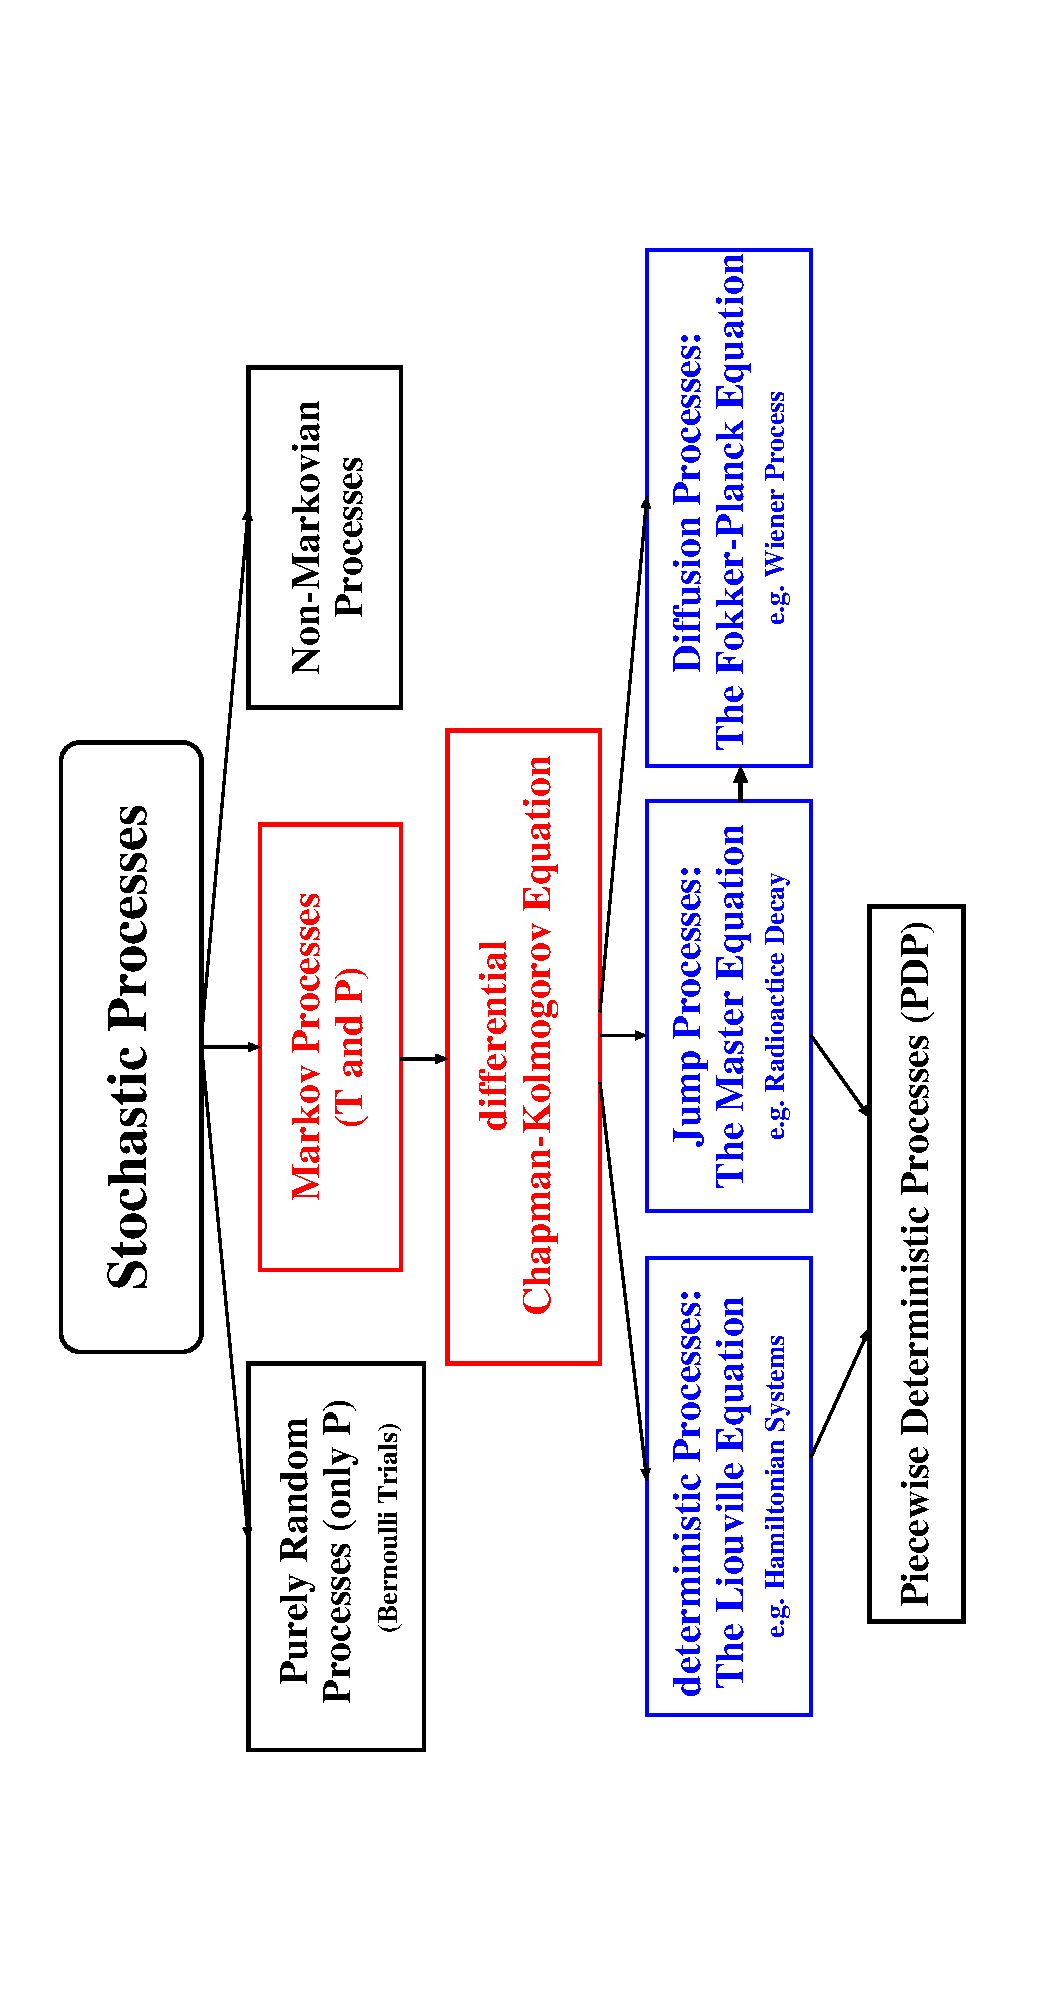
\includegraphics[width=10cm]{./Figures/f_chap4_overview.eps}
\caption{Overview of the theor of stochastic processes.}
\end{figure}

\section{The Liouville equation}
Let us consider a physical system whose dynamics is described
by a system of ordinary differential equations of first order
\begin{equation}
\label{ORDINARY_DIFF}
\frac{d}{dt} x(t) = g(x(t)),
\end{equation}
where $g$ is a function $R^d \rightarrow R^d$. 
It is clear that Hamiltonian systems belong to this class 
(\cite{ARNOLD}). The initial 
condition is
\begin{equation*}
x(0) = x \in R^d.
\end{equation*}
We denote the unique solution of this equation by $\phi(t,x)$,
where the $x$ stresses the dependence on the initial condition.

If $f:R^d \rightarrow R^d$ is a continuous differentiable function
then it follows from Eq. (\ref{ORDINARY_DIFF}) 
\begin{equation}\label{COORDINATE_FREE}
\frac{d}{dt} f(x(t)) = \sum_i \frac{\partial f}{\partial x_i}
          (x(t)) g^i(x(t)),
\end{equation}
where $g^i$ denotes the $i$--th component of $g$. 


With the help of these formal preliminaries it is easy to 
construct the generator of a deterministic Markov process.
Obviously we have for the expectation value
\begin{equation*}
Ef(x(t)) = f(\phi(x,t)),
\end{equation*}
where the symbol $E$ denotes the expectation value.

Inserting the above expectation value into the definition of a 
generator (\ref{DEF_GENERATOR}) we immediately obtain
\begin{eqnarray*}
{\cal{A}}_L(t) f & = & \lim_{t\rightarrow 0} \frac{1}{t}
                        \left[ Ef(x(t)) - f(x)\right] \\
             & = & \lim_{t\rightarrow 0} \frac{1}{t}
                        \left[ f(\phi(x,t)) - f(\phi(0,x))\right] \\
              & = & \frac{d}{dt} f(x) ,
\end{eqnarray*}
and finally, using Eq. (\ref{COORDINATE_FREE}),
\begin{equation*}
{\cal{A}}_L(t) f = \sum_i \frac{\partial f}{\partial x_i}(x) g^i(x).
\end{equation*}


Having determined the generator it is now straightforward to 
evaluate the corresponding differential Chapman--Kolmogorov 
equation. To this end we only 
have to determine the operator which is adjoint to
${\cal{A}}_L$ by partial integration. It is evident that we have
\begin{eqnarray}
\label{GEN_DET0}
\int dx \left[{\cal{A}}_L f(x) \right]h(x) &=&
          \sum_i \int dx \left[g^i 
           \frac{\partial f}{\partial x_i} \right] h(x) \nonumber \\
     & = & -\sum_i f \frac{\partial}{\partial x_i} g^i h(x).      
\end{eqnarray}
Since Eq. (\ref{GEN_DET0}) holds for any function $h(x)$
\begin{equation}
\label{GEN_DET_A}
{\cal{A}}_L^{\dagger} h(x) = -\sum_i \frac{\partial}{\partial x_i}
    \left(g_i h(x) \right).
\end{equation}
Inserting (\ref{GEN_DET_A}) into the differential Chapman--Kolmogorov 
equation
(\ref{KOL_FORWARD}) 
leads to the master equation for a deterministic Markov process
\begin{equation}
\frac{\partial}{\partial t} T(x,t|x',t') =
 - \sum_i \frac{\partial}{\partial x_i}
     \left(g_i(x)T(x,t|x',t')  \right).
\end{equation}
In statistical physics the above equation is called the Liouville 
equation.
 
The Liouville equation is the starting point for the microscopic 
description of matter for classical as well as for quantum 
mechanical systems. It is one of the fundamental equations of 
statistical physics. 

\subsection{Example: Classical statistical mechanics}
In order to give an example of the occurrence
of the Liouville equation we consider a closed classical system
with $N$ degrees of freedom, e.g., $N$ particles in a 
three--dimensional box. We know from classical mechanics, that the 
state  of such a system is completely specified by the set of $6N$
independent variables $\vec{p}^N=(\vec{p}_1, \ldots, \vec{p}_N)$ 
and $\vec{q}^N=(\vec{q}_1, \ldots, \vec{q}_N)$, where $\vec{p}_i$
and $\vec{q}_i$ denote the momentum and the position of the 
$i$--th particle. 

If the system is Hamiltonian (\cite{ARNOLD}), 
i.e., if we can define a Hamiltonian
$H(\vec{p}^N,\vec{q}^N)$, then the time evolution of the momentum 
and of the position of the particles is given by Hamilton's 
equations of motion
\begin{eqnarray*}
\frac{d}{dt} \vec{p}_i &=& - \frac{\partial H}{\partial \vec{q}_i} 
             \\
\frac{d}{dt} \vec{q}_i &=&  \frac{\partial H}{\partial \vec{p}_i} 
.
\end{eqnarray*}

In a real physical system it is not possible to specify exactly 
the state of the system. There is always some uncertainty in the 
initial conditions. Therefore, we regard $(\vec{p}^N,\vec{q}^N)$
as a stochastic variable which is initially distributed according 
to the joint probability density $P^N(\vec{p}^N,\vec{q}^N,0)$. 
The dynamics of this probability distribution
is described by the following 
Liouville equation
\begin{equation*}
\frac{\partial}{\partial t} P^N =  {\cal{A}}_L^{\dagger} P^N,
\end{equation*}
where
\begin{equation*}
{\cal{A}}_L^{\dagger} = -\sum_{i=1}^N \left( 
      \frac{\partial H}{\partial \vec{p}_i} 
            \cdot \frac{\partial}{\partial \vec{q}_i} 
         - \frac{\partial H}{\partial \vec{q}_i} 
             \cdot \frac{\partial}{\partial \vec{p}_i}.
      \right)
\end{equation*}
The Liouville equation is often written in the following form
\begin{equation*}
i \frac{\partial}{\partial t} P^N(\vec{p}^N,\vec{q}^N,t) =  
  {\cal{L}} P^N(\vec{p}^N,\vec{q}^N,t),
\end{equation*}
where
\begin{equation*}
{\cal{L}} =  i {\cal{A}}_L^{\dagger}.
\end{equation*}
The operator ${\cal{L}}$ is called the Liouville operator.
If the probability disribution at time $t=0$ is known the above 
Liouville equation may be integrated formally  
to find the probability density
at later times $t$
\begin{equation*}
P^N(\vec{p}^N,\vec{q}^N,t) = \exp(-i {\cal{L}}t)  
P^N(\vec{p}^N,\vec{q}^N,0).
\end{equation*}
The Liouville equation is the starting point for the evaluation of 
probability distributions in statistical mechanics. Extensive use 
of the Liouville equation is done in kinetic theory. From the 
Liouville equation it is possible to derive a hierarchy of 
equations for probability densities, the so--called 
BBGKY--hierarchy from which kinetic equations may be derived
(\cite{REICHL}).


\section{The master equation}
Let us now introduce jump processes (\cite{DAVIES,FELLER}).
We consider a system in a given state $x$.  
In order to characterize a jump process, i.e., a process
in which the system undergoes sudden discontinuous changes of its state,
we have to specify the probability for 
the system to remain in $x$ during the time interval $dt$ 
\begin{equation*}
(1-\lambda(x) dt)
\end{equation*}
and the probability that the system jumps from state $x$ to state
$x'$ during the time interval $dt$ 
\begin{equation*}
\lambda(x) Q(x',x) dt,
\end{equation*}
where
\begin{equation}
\label{NORM_Q}
\int dx' Q(x',x) =1.
\end{equation}
Then,
\begin{equation*}
Ef(x(dt+t)) = (1-\lambda(x)dt) f(x)
   + \lambda(x) dt \int dx'f(x') Q(x',x).
\end{equation*}
From the definition of the generator we obtain immediately the
generator of the jump process
\begin{equation}
\label{GEN_JUMP}
{\cal{A}}_M f(x) = \lambda(x) \int dx' \left( f(x') 
-f(x)\right)Q(x',x),
\end{equation}
where we made use of Eq. (\ref{NORM_Q}).
Again, in order to derive the Kolmogorov forward equation we have 
to construct the adjoint operator to ${\cal{A}}_M$.
We start from Eq. (\ref{KOL_FORWARD_0})  
\begin{equation}
\label{KOL_FORWARD_J0}
\int dx \left[ {\cal{A}}_M(t) f(x) \right] T(x,t|x',t') =
  \int dx f(x) \frac{\partial}{\partial t} T(x,t|x',t').
\end{equation}
and insert the generator (\ref{GEN_JUMP}) into the left--hand side 
of the above equation
\begin{eqnarray*}
\lefteqn{\int dx \left[ {\cal{A}}_M(t) f(x) \right] T(x,t|x',t')} 
\\
&=& \int dx \left[ \lambda(x)
       \int dx'' \left(f(x'') -f(x) \right) Q(x'',x) \right] T(x,t|x',t') 
       \\
& = & \int dx \int dx'' \lambda(x) f(x'') Q(x'',x) T(x,t|x',t') \\
& & - \int dx \int dx'' \lambda(x) f(x) Q(x'',x) T(x,t|x',t').
\end{eqnarray*}
By renaming $x \rightarrow x''$ and $x'' \rightarrow x$  in the first line of the
above equation we get
\begin{eqnarray}
\label{ADJOINT_JUMP}
\lefteqn{\int dx  f(x) \int dx'' \lambda(x'')  Q(x,x'') T(x'',t|x',t')}
     \nonumber \\
& & - \int dx f(x) \int dx'' \lambda(x)  Q(x'',x) T(x,t|x',t') \nonumber \\
& \equiv & \int dx f(x) \left[ {\cal{A}}_M^{\dagger}(x) 
          T(x,t|x',t')      \right]
\end{eqnarray}
From Eq. (\ref{KOL_FORWARD_J0}) and from Eq. (\ref{ADJOINT_JUMP}) 
we conclude that the differential Chapman--Kolmogorov equation 
of a jump process
reads
\begin{eqnarray} 
\label{KOL_FORWARD_J1}
\lefteqn{\frac{\partial}{\partial t} T(x,t|x',t') =} \nonumber \\ 
&& \int dx'' \lambda(x'') Q(x,x'') T(x'',t|x',t')
 - \int dx'' \lambda(x) Q(x'',x) T(x,t|x',t').
\end{eqnarray}
Because of Eq. (\ref{NORM_Q}) we can write the above equation also 
in the form
\begin{eqnarray} 
\label{KOL_FORWARD_J2}
\lefteqn{\frac{\partial}{\partial t} T(x,t|x',t') =} \nonumber \\ 
&& \int dx'' \lambda(x'') Q(x,x'') T(x'',t|x',t')
 - \lambda(x) T(x,t|x',t').
\end{eqnarray}
Usually the differential Chapman--Kolmogorov equation for a jump process is 
written in a more suggestive form. To this end we introduce the 
total transition rate pro time unit for a transition from state $x'$ 
into  state $x$ to occur
\begin{equation*}
w(x,x') = \lambda(x') Q(x,x')
\end{equation*}
and write the differential Chapman--Kolmogorov equation 
for a jump process in its final form
\begin{equation}
\label{MASTER_JUMP}
\frac{\partial}{\partial t} T(x,t|x',t') =
 \int dx'' \left( w(x,x'') T(x'',t|x',t')
 - w(x'',x) T(x,t|x',t') \right).
\end{equation}
The above equation is called the master equation. 
The name master equation appears for the first time in a paper by
Nordsieck, Lamb and Uhlenbeck (\cite{NORDSIECK}). 
It was chosen to denote an equation from which
all relevant equations and results can be derived. 

In the physical literature Eq. (\ref{MASTER_JUMP}) is written in 
the simplified form
\begin{equation}
\label{MASTER_JUMP_P}
\frac{\partial}{\partial t} P(x,t) =
 \int dx'' \left( w(x,x'') P(x'',t)
 - w(x'',x) P(x,t) \right).
\end{equation}
This equation has the following meaning (\cite{VAN_KAMPEN}). Take a 
time $t'$ and a state $x'$ and consider 
the solution of Eq. (\ref{MASTER_JUMP_P})
for $t \ge t'$ with the initial condition $P(x,t') = 
\delta(x-x')$. This solution is the conditional transition 
probability $T(x,t|x',t')$ of the Markov process for each choice
of $x'$ and $t'$. It is important to keep in mind that 
Eq. (\ref{MASTER_JUMP_P})
is always to be interpreted as an equation for $T$ and not for 
$P$.

In the above form the physical meaning of the master equation is 
also evident. The master equation is a balance equation for the
probability to find the system in some state. The first term in 
the master equation describes the gain of state due to transitions 
from the other states. The second term is the loss due to the 
transitions from the given state into the others. Evidently,
the term with $x=x'$ does not contribute to the integral.

If the state space of the stochastic process is discrete, i.e.
all integer numbers $n$,
the master equation for the time evolution of $P(n,t)$ will assume 
the following discrete form
\begin{equation}
\label{MASTER_JUMP_P_N}
\frac{\partial}{\partial t} P(n,t) =
 \sum_{n'} \left( w(n,n') P(n')
 - w(n',n) P(n,t) \right).
\end{equation}
We will discuss in the next section how the stochastic processes 
defined in terms of a master equation can be simulated 
numerically.


\section{Stochastic simulation}
In principle there are two ways to treat numerically
stochastic processes which are defined in terms of master
equations. In the first approach one solves numerically the
master equation as a differential equation for the probability
density. Although this deterministic method is direct we will not consider it 
here for the following reason. It  turns out that the direct 
numerical solution of the master equation is not particularly 
efficient from a computational point of view. The second approach,
which we will introduce in this section relies upon the simulation 
of the underlying stochastic process. In other words one considers 
a particle and lets it jump from one state to another with certain 
given transition rates. Such a procedure is called the generation 
of a realization of the stochastic process. If a sufficiently 
great number of realizations has been generated the interesting 
statistical quantities can be evaluated as ensemble averages.

In fact the numerical performance of the direct approach gets 
worse compared to the stochastic simulation with increasing 
dimension of the system considered. We already met a similar 
situation, when we considered numerical algorithms for the 
computation of integrals. There the direct integration of 
multidimensional integrals turned out to be less efficient than 
the Monte--Carlo integration.

In order to formulate a stochastic simulation algorithm we 
consider for simplicity the master equation of a one--step 
process. Sometimes such processes are also called birth--and--death
processes. The range of such processes consists of all integers
$n$ and the matrix of the transition probabilities per unit time
allows only jumps between adjacent sites
\begin{equation*}
w(n',n) \neq 0 \;\;\; \text{for} \;\;\; n'=n \pm 1
\end{equation*}
and
\begin{equation*}
w(n',n) = 0 \;\;\; \text{otherwise}.
\end{equation*}
Exploiting the above structure we can write the master equation 
for the discrete one--dimensional process (\ref{MASTER_JUMP_P_N})
\begin{eqnarray*}
\dot{P}(n,t) &=& w(n,n+1)P(n+1,t) + w(n,n-1)P(n-1,t) \\
       && -w(n+1,n)P(n,t) -w(n-1,n)P(n).
\end{eqnarray*}
Now it is convenient to introduce the following notation
\begin{eqnarray*}
r(n+1) \equiv w(n,n+1) \\
g(n-1) \equiv w(n,n-1),
\end{eqnarray*}
so that the master equation for a general one--step process 
may be written in the following 
suggestive form
\begin{equation}
\label{MASTER_ONE_STEP}
\dot{P}(n,t) = r(n+1)P(n+1,t) + g(n-1)P(n-1,t)
        -[r(n)+ g(n)]P(n,t).
\end{equation}

Let us now assume that at time $t$ the particle is in state
$n$. The total transition rate to leave this state, i.e. to jump 
out of this state either to state $n+1$ or to state $n-1$, is 
given by
\begin{equation}
\label{TOTAL_RATE_ONE_JUMP}
\lambda(n) = r(n) + g(n).
\end{equation}
As we already know  the quantity $\lambda(n) dt$ is the 
probability that the next jump occurs within the infinitesimal 
time step $dt$. Accordingly the probability that the next jump 
occurs after $(N+1)$ time steps $dt$ is given by
\begin{equation*}
q=[1-\lambda(n)dt]^N \lambda(n)dt,
\end{equation*}
where $[1-\lambda(n)dt]^N$ denotes the probability that no jump
occurs during the first $N$ steps. We now write $(N+1)dt =t$, so 
that we have
\begin{equation*}
q= \left( 1 - \frac{\lambda(n) t}{N+1}\right)^N \lambda(n) dt.
\end{equation*}
We now perform the limit $dt \rightarrow 0$ for fixed $t$. This 
limit implies, of course, $N \rightarrow \infty$ and hence the 
probability that a jump occurs after time $t$ is given by
\begin{equation*}
q= \lambda \exp(-\lambda t) dt = f(t) dt.
\end{equation*}
The waiting time distribution for the time of the next jump is an
exponential distribution.
It is now clear what we have to do in order to determine the time 
of the next jump in the stochastic simulation.  
We simply have to draw random times $\tau$, 
which are distributed according to the density $f(t)$. Since $f(t)$
is an exponential distribution, these random times can easily be 
drawn with the help of the inversion method
\begin{equation}
\label{TAU_ONE_STEP}
\tau = - \frac{1}{\lambda(n)} \log(\xi),
\end{equation}
where $\xi$ is a uniformly distributed random number on the 
interval $[0,1)$. 

Having determined the stochastic time of the
next jump we still have to decide which transition actually takes 
place. We have only two possibilities: In case of a jump the 
particle can reach the state $(n-1)$ with probability
\begin{equation*}
y_1 = \frac{r(n)}{\lambda(n)}
\end{equation*}
or the state  $(n+1)$ with probability
\begin{equation}
y_2 = 1 -y_1 = \frac{g(n)}{\lambda(n)}.
\end{equation}
Thus, the algorithm for the simulation of a one--step--process
reads: \\

(i) Draw a uniformly distributed random number $\xi_1$ on $[0,1)$
   and compute the random jump time $\tau$ according to 
   (\ref{TAU_ONE_STEP}). 
   
(ii) Draw a uniformly distributed random number $\xi_2$ on 
$[0,1)$. If the condition $(\xi_2 < y_1)$ is satisfied we set 
$\nu =+1$.  Otherwise we set $\nu =-1$.

(iii) Advance the process
\begin{eqnarray*}
t &\longrightarrow& t+\tau \\
n & \longrightarrow & n + \nu.
\end{eqnarray*}

The flow chart of the algorithm can be seen in Fig. 
(\ref{F_ONESTEP_ALGORITHM}).
\begin{figure}
\label{F_ONESTEP_ALGORITHM}
\includegraphics[width=7cm]{./Figures/f_onestep_algorithm.eps}
\caption{Flow chart of a stochastic simulation of a 
    one--step process. The symbols used
     are explained in the text.}
\end{figure}
The algorithm has been implemented in the program {\texttt{onestep.m}}
whose listing can be seen below. The program {\texttt{onestep.m}} makes
use of a function called {\texttt{decayymaster.m}} in which the
transitions rates $g(n)$ and $r(n)$ are specified. In the 
following subsection we will discuss three typical one--step 
processes. The specific form of the function \texttt{decaymaster} 
will be given there.

\subsubsection{Listing of the program {\texttt{onestep.m}}}
\inputlisting{./Listings/onestep.m}

The program will be applied in the next subsections.


\subsection{Radioactive decay}
As a first example we consider the master equation 
description of the radioactive decay. To this end let
$P(n,t)$ be the probability density to find $n$ radioactive nuclei
at time $t$. The probability for a nucleus to decay in unit time will
be denoted by $\gamma$. The radioactive decay is a typical example
of a one--step process. It is defined through
the transition rates
$g(n) \equiv 0$ and $r(n)= \gamma n$, where $\gamma$ is the decay constant.
Substitution of the above $g(n)$ and $r(n)$ into the master equation
for the one--step process
(\ref{MASTER_ONE_STEP}) yields the master equation of the radioactive 
decay
\begin{equation}
\frac{\partial}{\partial t} P(n,t) = 
\gamma (n+1) P(n+1,t) - \gamma n P(n,t).
\end{equation}
Before we apply the stochastic simulation algorithm to the 
generation of trajectories of the stochastic process we consider
for one moment the above master equation.

The above equation has to be solved for the initial condition
$P(n,0)= \delta(n,n_0)$. 
It is interesting to establish the
relation between the master equation and the macroscopic 
description in terms of differential equations we already met in 
the introduction.
To this end we consider
\begin{eqnarray*}
\sum_{n=0}^{\infty} n \dot{P}(n,t) &=&
       \gamma \sum_{n=0}^{\infty} n(n+1)P(n+1) 
         - \gamma  \sum_{n=0}^{\infty} n^2 P(n) \\
  &=& \gamma \sum_{n=0}^{\infty} (n-1)n P(n) 
         - \gamma  \sum_{n=0}^{\infty} n^2 P(n) \\
  & = & - \gamma \sum_{n=0}^{\infty} n P(n) .
\end{eqnarray*}
Thus we have found the following dynamical equation for the 
average of the stochastic 
variable $N(t)$
\begin{equation}
\frac{d}{dt} \langle N(t) \rangle = - \gamma \langle N(t) \rangle.
\end{equation}
Note that the mean value of the stochastic process obeys the 
differential equation for the concentration. It is clear that the 
above equation has the following solution for the initial value
$\langle N(0)\rangle = n_0$
\begin{equation*}
\langle N(t) \rangle = n_0 \exp(-\gamma t).
\end{equation*}

Let us now turn to the stochastic simulation. In order to use
the program \texttt{onestep.m} we still have to specify
the function \texttt{decaymaster.m}. The listing of this
function can be seen below.
\subsubsection{Listing of the function {\texttt{decaymaster.m}}}
\inputlisting{./Listings/decaymaster.m}

Now we are in the position to simulate the stochastic process of
radioactive decay. We run the program for the following parameters
\texttt{n0=500}, \texttt{tend=30}, and \texttt{nreal=10}.
The decay rate is $\gamma=0.1$.
The result of the simulation can be seen in Fig. (\ref{F_OS_DECAY}).

\begin{figure}
\label{F_OS_DECAY}
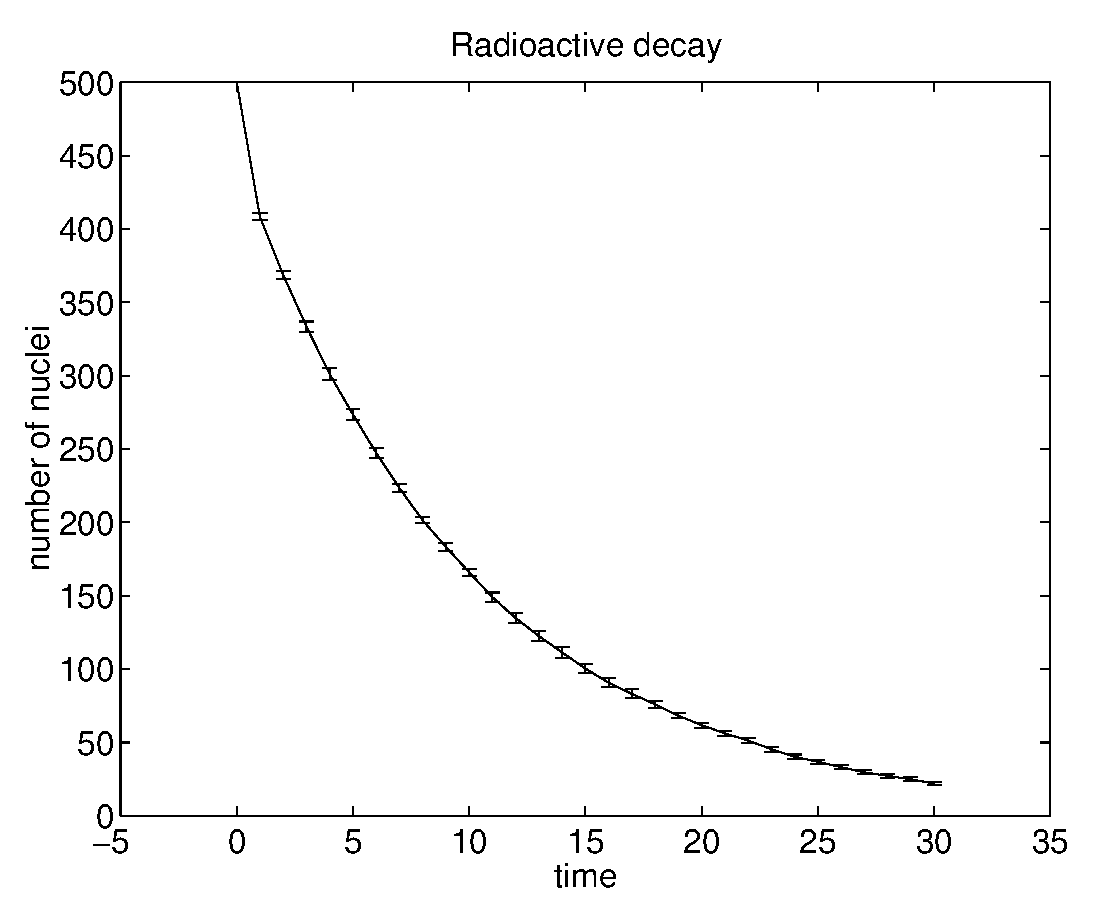
\includegraphics[width=10cm]{./Figures/f_os_decay.eps}
\caption{Stochastic simulation of radioactive decay. The initial
  number of decaying nuclei is {\texttt n0}$= 100$. {\texttt tend}
is 30 and the ensemble average was taken over 10 realizations.
The decay rate is $\gamma=0.1$.}
\end{figure}  

\subsection{The Poisson process}
A further important one--step process is the Poisson process, which
is defined by
\begin{equation}
r(n) = 0; \;\;\; g(n) = q = \text{const}.
\end{equation}
Inserting the above transition rates into the master equation
(\ref{MASTER_ONE_STEP}) we get the master equation defining
the Poisson process
\begin{equation}
\label{MASTER_POISSON}
\frac{\partial}{\partial t} P(n,t|n',t') =
  q [ P(n-1,t|n',t') - P(n,t|n',t')].
\end{equation}
The Poisson process describes a random walk over the integers
$0,1,2,\ldots$. The steps of the walk are all of length $l$ and are 
only to the right. They are performed at random times with 
probability per unit time equal to $q$.

It is instructive to consider the analytical solution of the 
above master equation (\ref{MASTER_POISSON}). The analytical
solution will be constructive with the help of a very useful 
technique which is based upon the characteristic function
\begin{equation*}
G(s,t) = \langle \exp(ins)\rangle = \sum_n P(n,t|n',t') \exp(ins).
\end{equation*}
The  equation of motion for the characteristic function is easily 
obtained with the help of (\ref{MASTER_POISSON}). We find
\begin{equation*}
\frac{\partial}{\partial t} G(s,t) = 
       q \left[ \exp(is) -1 \right] G(s,t).
\end{equation*}
Assuming that at time $t'$ the one--sided random walk starts at
$n'=0$, the initial condition of the above differential equation
reads
\begin{equation*}
G(s,0) = 1.
\end{equation*}
In this case the solution of the above differential equation of 
motion  for the characteristic function is easily found. It reads
\begin{equation*}
G(s,t) = \exp\left\{ tq \left[ \exp(is)-1 \right]\right\}.
\end{equation*}
To read out the analytical solution for the transition probability
$P(n,t|0,0)$ it is convenient to write the above solution in the
form
\begin{eqnarray*}
G(s,t) &= & \exp(-tq) \exp \left[ tq \exp(is)\right] \\
       &= & \sum_{n=0}^{\infty} \exp(-tq) 
             \frac{[tq\exp(is)]^n}{n!}.
\end{eqnarray*}
For $s=0$ and from the definition of the characteristic function
it follows immediately that
\begin{equation*}
P(n,t|0,0) = \exp(-tq) \frac{(tq)^n}{n!},
\end{equation*}
which evidently is a Poisson distribution. As we know the 
characteristic function allows the determination of all moments of 
the stochastic process through the relation
\begin{equation*}
\langle n^m(t) \rangle = \left. 
       \left( -i \frac{\partial}{\partial s} \right) G(s,t)  
       \right|_{s=0}.
\end{equation*}
Applying the above formula we find
\begin{equation*}
\langle n(t) \rangle = qt
\end{equation*}
and
\begin{equation*}
\langle n^2(t) \rangle = qt + (qt)^2.
\end{equation*}
Accordingly, the variance of the Poisson process is given by
\begin{equation*}
\text{Var}(n) = \langle n^2(t) \rangle - \langle n(t) \rangle^2 = 
   qt.
\end{equation*}
The simulation of the Poisson process is straightforward. We make 
use of the program \texttt{onestep.m} and simply write a new 
function \texttt{poissonmaster.m} according to the 
master equation (\ref{MASTER_POISSON}) whose listing can be
seen below.

\subsubsection{Listing of the function {\texttt{poissonmaster.m}}}
\inputlisting{./Listings/poissonmaster.m}

To begin we generate one realization of the Poisson process. To 
this end we run the program with the following parameters:
\texttt{nstart=0}, \texttt{tend=30}, \texttt{nreal=1}. In the 
function \texttt{poissonmaster} we have chosen the transition rate
to be \texttt{q=1}. One realization of the Poisson process can be
seen in Fig. (\ref{F_OS_POI_R}).
\begin{figure}
\label{F_OS_POI_R}
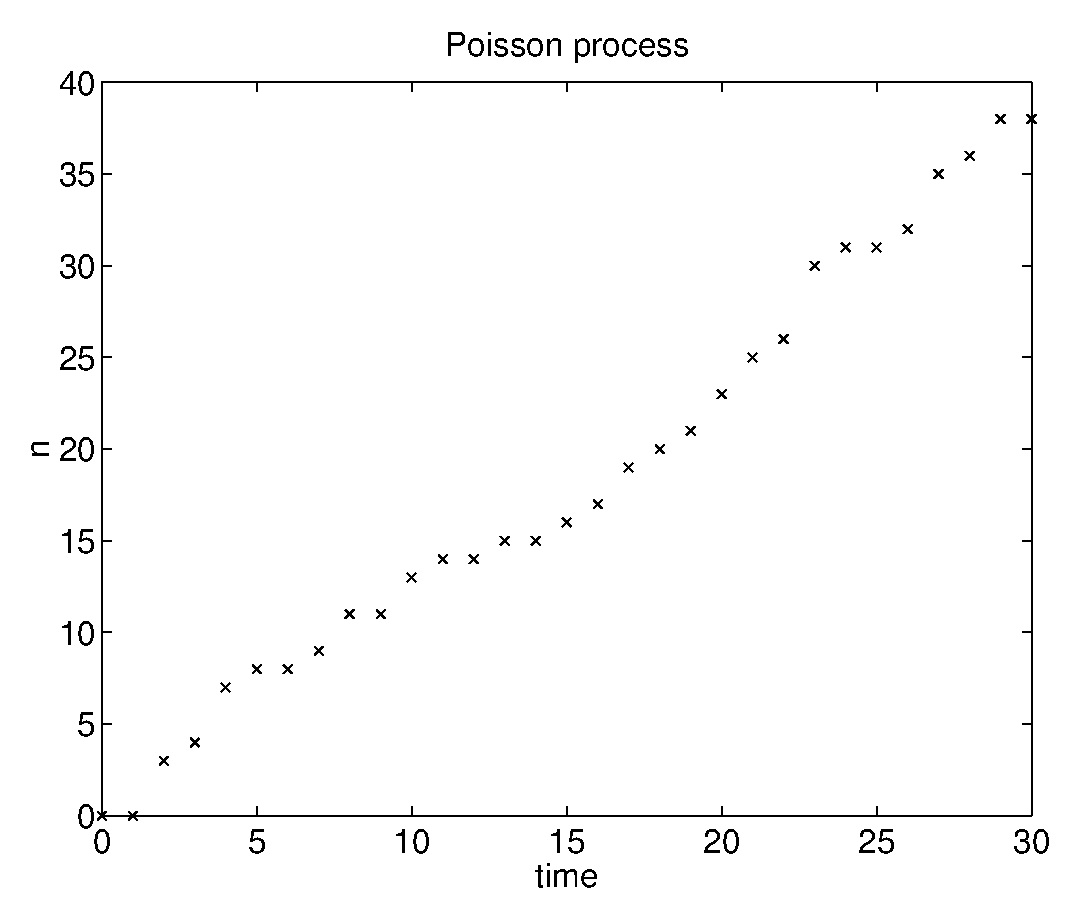
\includegraphics[width=10cm]{./Figures/f_os_poi_r.eps}
\caption{Stochastic simulation of the Poisson process. The 
one--sided random walk starts at \texttt{nstart=0}.  
{\texttt tend} is 30 and \texttt{nreal=1}.
The jump rate is \texttt{q=1}.}
\end{figure}  
In Fig. (\ref{F_OS_POI_1}) we show an ensemble average over 20
realizations of the Poisson process. The other parameters are 
unchanged.
\begin{figure}
\label{F_OS_POI_1}
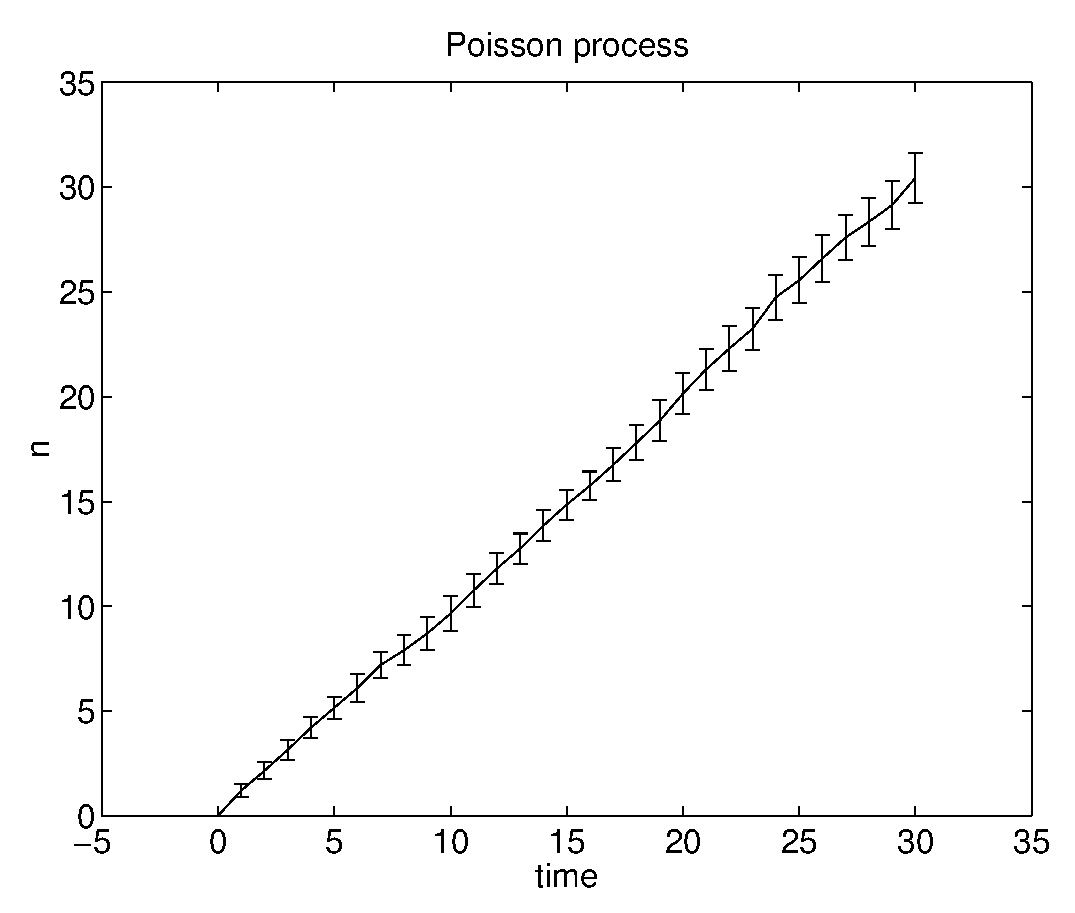
\includegraphics[width=10cm]{./Figures/f_os_poi_1.eps}
\caption{Stochastic simulation of the Poisson process. The 
one--sided random walk starts at \texttt{nstart=0}.  
{\texttt tend} is 30 and \texttt{nreal=20}.
The jump rate is \texttt{q=1}.}
\end{figure}
It is interesting to consider the limit of continuous space for the
Poisson process. Let us denote the distance travelled by 
\begin{equation*}
x=nl.
\end{equation*}
As a function of the new stochastic variable $x$ the 
characteristic function $\tilde{G}$ is
\begin{equation*}
\tilde{G}(s,t) = \langle \exp(isx) \rangle = 
     \exp\{tq[\exp(ils)-1] \}.
\end{equation*}
We perform the limit $l \longrightarrow 0$ keeping 
\begin{equation*}
ql=v=\text{const}
\end{equation*}
and obtain keeping only the terms linear in $l$ in the Taylor
expansion of $\exp(ils)$
\begin{equation*}
\lim_{l\rightarrow 0}\tilde{G}(s,t) = \exp(itvs).
\end{equation*}
So, in the continuum limit the transition probability is
\begin{equation*}
P(x,t|0,0) = \delta(x-vt).
\end{equation*}
Thus, the Poisson process has a deterministic limit. This can also 
be seen by considering, that in the same limit the master equation
for the Poisson process turns into the Liouville equation
\begin{equation*}
\frac{\partial}{\partial t} P(x,t|0,0) = -v 
\frac{\partial}{\partial x} P(x,t|0,0),
\end{equation*}
whose solution is the deterministic process we have just derived.
This behaviour can also be seen in the simulation. To this end
we run the program \texttt{onestep} with the function 
\texttt{poissonmaster} choosing \texttt{q=10}. The result of the 
simulation can be seen in Fig. (\ref{F_OS_POI_2}).
\begin{figure}
\label{F_OS_POI_2}
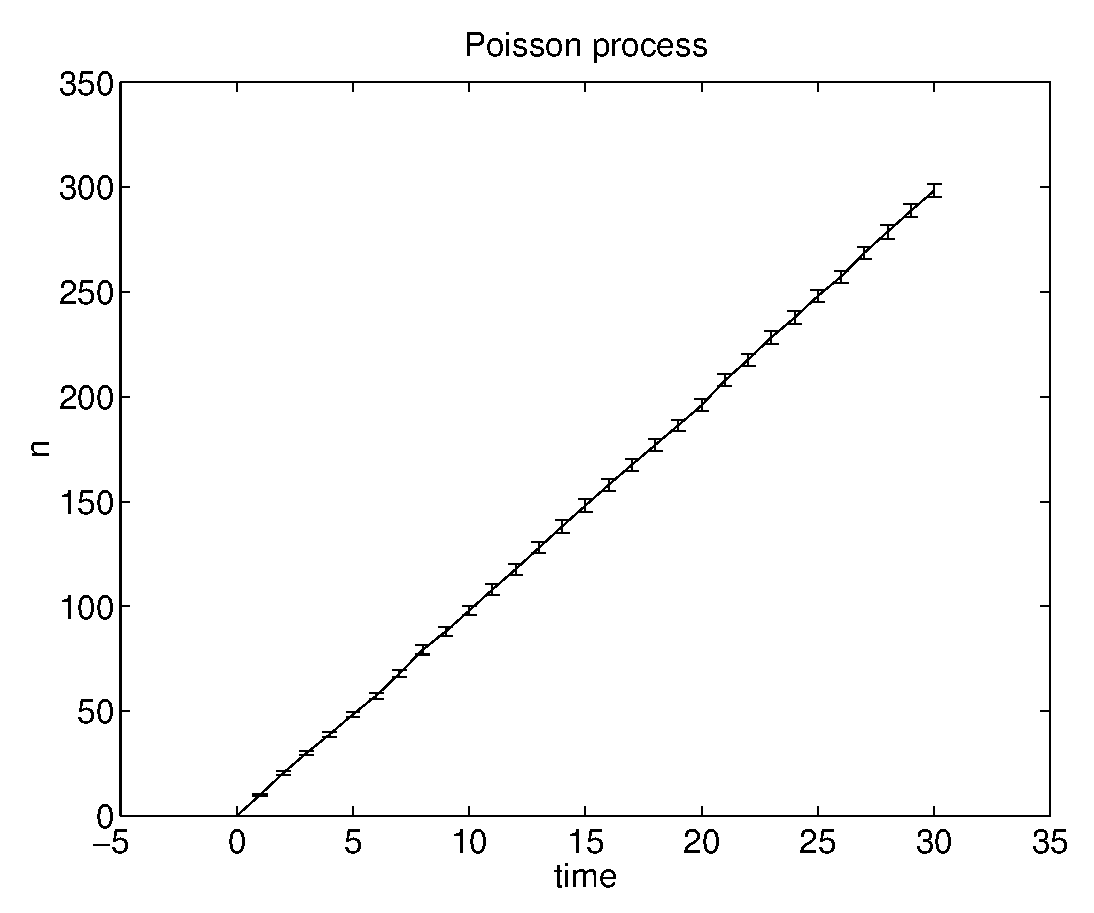
\includegraphics[width=10cm]{./Figures/f_os_poi_2.eps}
\caption{Stochastic simulation of the Poisson process. The 
one--sided random walk starts at \texttt{nstart=0}.  
{\texttt tend} is 30 and \texttt{nreal=20}.
The jump rate is \texttt{q=10}.}
\end{figure}
As we can see for a larger value of \texttt{q} the variance of the
process gets smaller. Thus the dynamics of the process is nearly 
deterministic.

\subsection{The continuous time random walk}
In this subsection we want to consider the master equation for
the one--dimensional random walk. The steps of the walker are of 
length $l$. The positions of the walker are $nl$ and are labelled
by the integer $n$. We already considered the random walk problem 
in Chapter 2.  There the walker was allowed to take steps 
to the left and to the right at some 
discrete times $N\tau$, where the time step $\tau$ was fixed.
Now, we consider a random walk which is continuous in time. The 
walker is allowed to take steps to the left or to the right with 
the probability per unit time $q$. This process is again described 
by a master equation for a one--step process (\ref{MASTER_ONE_STEP})
by choosing
\begin{equation*}
r(n) =g(n) =q.
\end{equation*}
Thus the master equation for the continuous time random walk
reads
\begin{eqnarray}
\label{MASTERWALK}
\frac{\partial}{\partial t} P(n,t|n',t') &=& 
       q \left\{ P(n+1,t|n',t') + P(n-1,t|n',t')\right. \\
       && \left.  - 2 P(n,t|n',t')  \right\}. \nonumber
\end{eqnarray}
Again the above master equation is easily solved with the help of 
the characteristic function $G(s,t)$. It is easy to check that the
characteristic function satisfies the equation
\begin{equation*}
\frac{\partial}{\partial t} G(s,t) = q [\exp(is) +\exp(-is) -2] G(s,t).
\end{equation*}
Assuming that the walker starts at time $t'=0$ in $n'=0$ we find
$G(s,0)=1$ and the solution of the above equation reads
\begin{equation*}
G(s,t) = \exp\{[ \exp(is) +\exp(-is) -2  ]tq\}.
\end{equation*}
With the help of the above expression for the characteristic 
function the moments are easily evaluated. We find
\begin{eqnarray*}
\langle n(t) \rangle &=& 0, \\
\langle n^2(t) \rangle &=& 2tq.
\end{eqnarray*}
Again we find the typical behaviour of a diffusive process.

The continuous time random walk is also easily simulated with the
help of the program \texttt{onestep}. To this end we have to write
a new function \texttt{walkmaster.m} which implements the 
appropriate transition rates.

\subsubsection{Listing of the function \texttt{walkmaster.m}}
\inputlisting{./Listings/walkmaster.m}

We run the program with the following parameters: 
\texttt{nstart=0}, \texttt{nreal=10}, \texttt{tend=30}, and
\texttt{q=1}. The result of the simulation can be seen in
Fig. (\ref{F_CTRW}).
\begin{figure}
\label{F_CTRW}
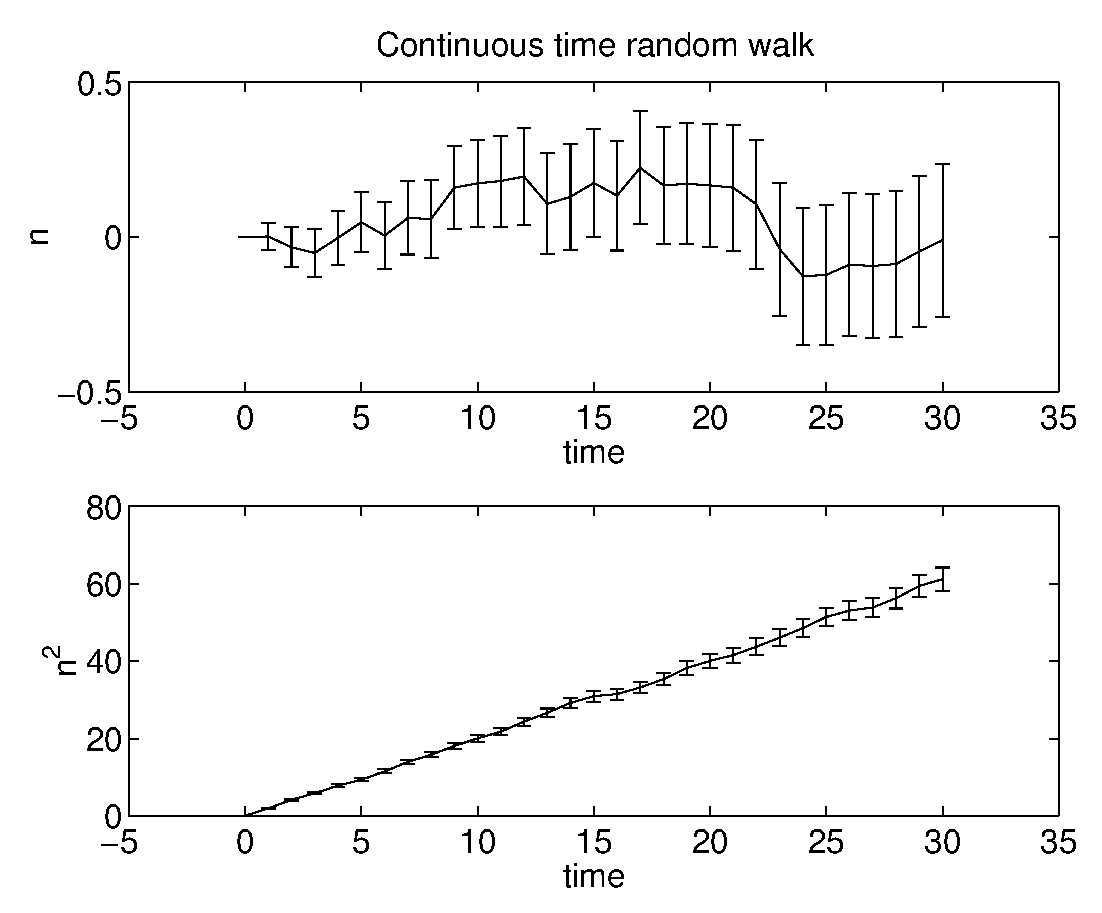
\includegraphics[width=10cm]{./Figures/f_ctrw.eps}
\caption{Stochastic simulation of the continuous time
random walk. The 
random walk starts at \texttt{nstart=0}.  
{\texttt tend} is 30 and \texttt{nreal=20}.
The jump rate is \texttt{q=1}.}
\end{figure}

It is of particular interest to look at the continuous space limit
of the continuous time random walk. Again we write for the 
distance travelled by the walker $x=nl$. The characteristic
function as a function of $x$ reads
\begin{eqnarray*}
\tilde{G}(s,t) &=& G(sl,t) = \langle \exp(ixs) \rangle \\
                &=& \exp\{[\exp(ils) + \exp(-ils)-2]tq \}.
\end{eqnarray*}
The limit of infinitesimally small steps $l \longrightarrow 0$ 
leads to
\begin{equation}
\label{CHAR_WALK_X}
\tilde{G}(s,t) = \exp(-s^2tD),
\end{equation}
where
\begin{equation*}
D=\lim_{l\rightarrow 0} (l^2q).
\end{equation*}
The quantity $D$ can be interpreted as the mean square distance 
traveled  per unit time.  The characteristic function (\ref{CHAR_WALK_X})
is the characteristic function of a Gaussian process of the form
\begin{equation*}
P(x,t|0,0) = \frac{1}{(4\pi Dt)^{1/2}} \exp\left( -x^2/4Dt 
\right).
\end{equation*}
This is the transition probability of a so--called {\em Wiener process},
which can be regarded as a continuous time random walk in the 
limit of infinitesimally small step size. We will consider the 
Wiener process in more detail in the next section.

The following remark may serve as an introduction to the next 
section. Of course, we can also expand directly the master equation
(\ref{MASTERWALK}) as a function of $x$ up to second order terms 
in $l$ and get
\begin{equation*}
\frac{\partial}{\partial t} P(x,t|0,0) =
     (l^2q) \frac{\partial^2}{\partial x^2} P(x,t|0,0),
\end{equation*}
which is a special type of Fokker--Planck equation, as we will see 
in the next section.

\section{The Fokker--Planck equation}
In this section we want to derive the Fokker--Planck equation
(\cite{RISKEN}),
which is a special type of master equation (\cite{VAN_KAMPEN})
in the limit of small jumps.
We begin by expressing the transition probability $w$ as a 
function of the size $r$ of the jump and of the starting point
\begin{equation*}
w(y,y') = w(y';r); \;\;\; r=y-y'.
\end{equation*}
The master equation (\ref{MASTER_JUMP_P}) then reads
\begin{equation}
\label{MASTER_SMALL_JUMP}
\frac{\partial}{\partial t} P(y,t) =
  \int dr w(y-r;r)P(y-r,t) - \int dr w(y;-r)P(y,t).
\end{equation}
In order to consider the limit of small jumps essentially
two assumptions will be needed. The first is that
the function
$w(y;r)$ will be a sharply peaked function of $r$ and will
vary slowly with $y$. To be more precise we assume that a $\delta >0$
exists such that
\begin{eqnarray*}
w(y';r)  & \approx & 0 \;\;\; \text{for} \;\;\; |r|> \delta \\
w(y'+\Delta y;r) & \approx & w(y';r) \;\;\; \text{for} \;\;\; |\Delta y| < 
\delta.
\end{eqnarray*}
The second assumption is that the solution $P(y,t)$ of the master equation 
in this limit will be a slowly varying function of $y$.

If these assumptions hold it is safe to expand the shift from $y$
to $y-r$ in the first integral in 
Eq. (\ref{MASTER_SMALL_JUMP}) in a Taylor series
\begin{equation}
\label{MASTER_EXPAND}
\frac{\partial}{\partial t} P(y,t) = \sum_{\nu=0}^{\infty}
   \frac{(-1)^{\nu}}{\nu!} \left( \frac{\partial}{\partial y} 
   \right)^{\nu}
    \left\{  a_{\nu}(y) P(y,t) \right\}
    - P(y,t) \int_{-\infty}^{\infty} dr w(y;-r),
\end{equation}
where we have defined
\begin{equation*}
a_{\nu}(y) = \int_{-\infty}^{\infty} dr r^{\nu} w(y;r).
\end{equation*}
Since the zeroth term in the sum and the second term of 
Eq. (\ref{MASTER_EXPAND}) cancel the small jumps expansion 
of the master equation reads
\begin{equation}
\frac{\partial}{\partial t} P(y,t) = \sum_{\nu=1}^{\infty}
   \frac{(-1)^{\nu}}{\nu!} \left( \frac{\partial}{\partial y} 
   \right)^{\nu}
    \left\{  a_{\nu}(y) P(y,t) \right\}.
\end{equation}
The above expansion is called the Kramers--Moyal expansion. 
Formally, we can write
\begin{equation}
\frac{\partial}{\partial t} P(y,t) = {\cal{A}}_{KM}^{\dagger}(y)
         P(y,t),
\end{equation}
where we introduced the adjoint generator
\begin{equation*}
{\cal{A}}_{KM}^{\dagger}(y) = \sum_{\nu=1}^{\infty}
   \frac{(-1)^{\nu}}{\nu!} \left( \frac{\partial}{\partial y} 
   \right)^{\nu}
     a_{\nu}(y).
\end{equation*}
It is easy to show by partial integration that the corresponding
generator  reads
\begin{equation*}
{\cal{A}}_{KM}(y) = \sum_{\nu=1}^{\infty}
   \frac{1}{\nu!}  a_{\nu}(y)
    \left( \frac{\partial}{\partial y} 
   \right)^{\nu}.
\end{equation*}
It is clear that dealing with the {\em Kramers--Moyal} expansion will 
not be easier than dealing with the original master equation.

A particularly interesting and useful approximation to a jump process is 
obtained by keeping only terms up to the second order in $\nu$
\begin{equation}
\label{FOKKER_PLANCK}
\frac{\partial}{\partial t} P(y,t) =
-\frac{\partial}{\partial y} \left\{ a_1(y) P(y,t) \right\}
   + \frac{1}{2} \frac{\partial^2}{\partial y^2} 
      \left\{ a_2(y) P(y,t) \right\}.
\end{equation}
The above equation is called the {\em Fokker--Planck equation}.
The first term on the right--hand side is usually called the drift
term since it is essentially Liouvillian. The second term
on the right--hand side is the diffusion term. In a later section
we will learn how to deal with this equation.

\subsection{The Wiener process}
Let us consider the important special case 
of vanishing drift, i.e. $a_1=0$, and diffusion coefficient
equal to one, i.e. $a_2=1$. The generator takes the form 
\begin{equation}
\label{WIENER_GENERATOR}
{\cal{A}}_W = {\cal{A}}_W^{\dagger} = \frac{1}{2} 
     \frac{\partial^2}{\partial y^2},
\end{equation}
and it defines a Wiener process. We already met the corresponding
Fokker--Planck equation, 
when we considered the continuous space limit of the the 
continuous time random walk.
Now we want to write down this Fokker--Planck equation in the form
\begin{equation*}
\frac{\partial}{\partial t}T(w,t|w_0,t_0) =
  \frac{1}{2} \frac{\partial^2}{\partial x^2} T(w,t|w_0,t_0).
\end{equation*}
The above equation can easily be solved with the help of the 
characteristic function
\begin{equation*}
G(s,t) = \int dw T(w,t|w_0,t_0) \exp(isw),
\end{equation*}
where we have assumed that the initial condition on the transition 
probability is
\begin{equation*}
T(w,t_0|w_0,t_0) = \delta(w-w_0).
\end{equation*}
The characteristic function satisfies the equation
\begin{equation*}
\frac{\partial}{\partial t}G(s,t) = - \frac{1}{2} s^2 G(s,t),
\end{equation*}
whose solution is, given the initial condition $G(s,t_0)=\exp(isw_0)$, 
\begin{equation*}
G(s,t) = \exp\left[isw_0 -s^2(t-t_0)/2\right].
\end{equation*}
Performing the inverse Fourier transformation of the above 
expression we find the transition probability
\begin{equation}
\label{TRANS_WIENER}
T(w,t|w_0,t_0)= \frac{1}{[2 \pi (t-t_0)]^{1/2}}
     \exp\left[ -(w-w_0)^2/2(t-t_0)\right].
\end{equation}
Thus, the transition probability density is a Gaussian with
\begin{eqnarray*}
\langle W(t) \rangle &=& w_0 \\
\langle [W(t)-w_0]^2\rangle &=& t-t_0.
\end{eqnarray*}
An initially sharp peaked distribution spreads in time.
It is important to make some remarks on the Wiener process $W(t)$.

The mean square of the Wiener process diverges linearly with time.
As we already know this behaviour is typical for diffusion 
processes and the trajectories of the Wiener process are very 
variable. We will look at the trajectories of the Wiener process 
soon. 

Although the paths of the Wiener process are continuous they are 
not differentiable since the derivative at any point is 
almost certainly infinite (\cite{gardiner}).

The Wiener process plays a central role in the description of 
diffusion processes by means of stochastic differential equations.
The reason is that the increments of the Wiener process
\begin{equation*}
\Delta W_i \equiv W(t_i) - W(t_{i-1}) \equiv W_i -W_{i-1} 
\end{equation*}
are statistically independent. This can be seen in the following 
way. Let us consider the joint probability density
\begin{eqnarray*}
P(w_n,t_n; w_{n-1},t_{n-1}; \ldots ; w_0,t_0) &=&
\prod_{i=0}^{n-1} T(w_{i+1},t_{i+1}|w_i,t_i) P(w_0,t_0).
\end{eqnarray*}
Exploiting the explicit form of the transition probabilities
(\ref{TRANS_WIENER}) the above joint probability density can be 
cast in the following form
\begin{eqnarray*}
\lefteqn{P(w_n,t_n; w_{n-1},t_{n-1}; \ldots ; w_0,t_0) =} \\
& & \prod_{i=0}^{n-1} 
\left\{ \frac{1}{[2 \pi (t_{i+1}-t_i)]^{1/2}}
\exp[-(w_{i+1}-w_i)^2/2(t_{i+1}-t_i)]
\right\}
P(w_0,t_0).
\end{eqnarray*}
Expressed in terms of the increments $\Delta W_i$ the above 
equation reads
\begin{eqnarray*}
\lefteqn{
P(\Delta w_n,\Delta t_n; \Delta w_{n-1},\Delta t_{n-1}; \ldots ; w_0,t_0) =} \\
& &\prod_{i=1}^{n} 
\left\{ \frac{1}{[2 \pi \Delta t_i)]^{1/2}}
\exp[-\Delta w_i^2/2 \Delta t_i]
\right\}
P(w_0,t_0),
\end{eqnarray*}
where we have introduced the variables
\begin{equation*}
\Delta t_i = t_{i} - t_{i-1}.
\end{equation*}
Thus, the increments $\Delta W_i$ are evidently statistically
independent and are distributed according to
\begin{equation*}
P(\Delta w,\Delta t) = \frac{1}{[2 \pi \Delta t)]^{1/2}}
\exp[-\Delta w^2/2 \Delta t].
\end{equation*}

At this point it is convenient to introduce a short hand notation 
for Gaussian distributed random numbers. The Gaussian random 
variable $X$ with mean $m$ and variance $\sigma^2$ will be denoted
by
\begin{equation*}
X \equiv {\bf N}(m,\sigma^2).
\end{equation*}
In particular we will name the random variable $\xi$
\begin{equation*}
\xi \equiv {\bf N}(0,1)
\end{equation*}
the unit normal random variable. In this notation we can write
for the Wiener $W(t)$ process
\begin{equation*}
W(t) = {\bf N} ( W_0, (t-t_0) )
\end{equation*}
and for the increment $\Delta W$
\begin{equation*}
\Delta W(t) = {\bf N} (0, 
     \Delta t ).
\end{equation*}

For later convenience we give two rules concerning the 
transformation of Gaussian random variables. First, let $a$ and $b$
be two numbers, then we have
\begin{equation*}
a +b {\bf N}(m,\sigma^2) = {\bf N} ( a+bm, b^2\sigma^2).
\end{equation*}
In particular we have for a unit normal random variable
\begin{equation*}
a+b\xi = {\bf N}(a,b^2).
\end{equation*}
Second, if ${\bf N}(m_1,\sigma_1^2)$ and ${\bf N}(m_2,\sigma_2^2)$ 
are statistically independent, then
\begin{equation*}
{\bf N}(m_1,\sigma_1^2) + {\bf N}(m_2,\sigma_2^2) =
   {\bf N}(m_1+m_2,\sigma_1^2+\sigma_2^2).
\end{equation*}
The above rule expresses the fact that, as we know, that Gaussian 
random variables remain Gaussian distributed under addition.
The rules just given can be demonstrated with the help of the 
random variable transformation theorem.

With the help of the first above rule it is clear that the 
increment $\Delta W$ can be expressed as
\begin{equation*}
\Delta W = \sqrt{\Delta t} \xi,
\end{equation*}
where $\xi$ is the unit normal random variable.

Let us now generate numerically some realizations of the Wiener 
process. To this end we need a way of calculating for a given 
value of the Wiener process $W(t)$ at time $t$ the value of the
process at time $t+\Delta t$. We will present an algorithm which
is exact for any positive value of $\Delta t$ (\cite{GILLESPIE}).

The algorithm exploits the fact that we know analytically the
conditional transition probability density. $T(w,t|w',t')$ is a 
Gaussian  with  mean $w'$ and variance $\sigma^2=2(t-t')$.
Accordingly, given $W(t)$ the increment $\Delta W(t)$
\begin{equation}
\label{ADVANCE_WIENER}
W(t+\Delta t) = W(t) + \Delta W(t)
\end{equation}
is distributed according to a Gaussian with zero mean and variance
$\sigma^2=2\Delta t$. The above formula is the update formula
for the algorithm for the generation of realizations of the Wiener
process. The algorithm essentially consists of the following 
steps:

(i) Let $W(t)$ be given.

(ii) Draw a Gaussian distributed random number $\Delta W$
with zero mean and variance $\sigma^2=2\Delta t$).

(iii) Advance the stochastic process according to the formula
(\ref{ADVANCE_WIENER}).

(iv) Goto (i) until the desired final time is reached.

A flow diagram of the program \texttt{wiener.m} can be seen in 
Fig. (\ref{F_WIENER_ALGORITHM}). 
\begin{figure}
\label{F_WIENER_ALGORITHM}
\includegraphics[width=6cm]{./Figures/f_wiener_algorithm.eps}
\caption{Flow diagram of the program \texttt{wiener.m}}
\end{figure}
\subsubsection{Listing of the function \texttt{wiener.m}}
\inputlisting{./Listings/wiener.m}

Let us run the program two times with the following parameters
\texttt{xstart=0}, \texttt{tend=50}, \texttt{deltat=0.01}, 
\texttt{nreal=1} in order to generate two realizations of the 
Wiener process. The two independent realizations can be seen 
on Figs. (\ref{F_WIENER_R1}) and (\ref{F_WIENER_R2}). The great 
variability of the realizations is evident. 
\begin{figure}
\label{F_WIENER_R1}
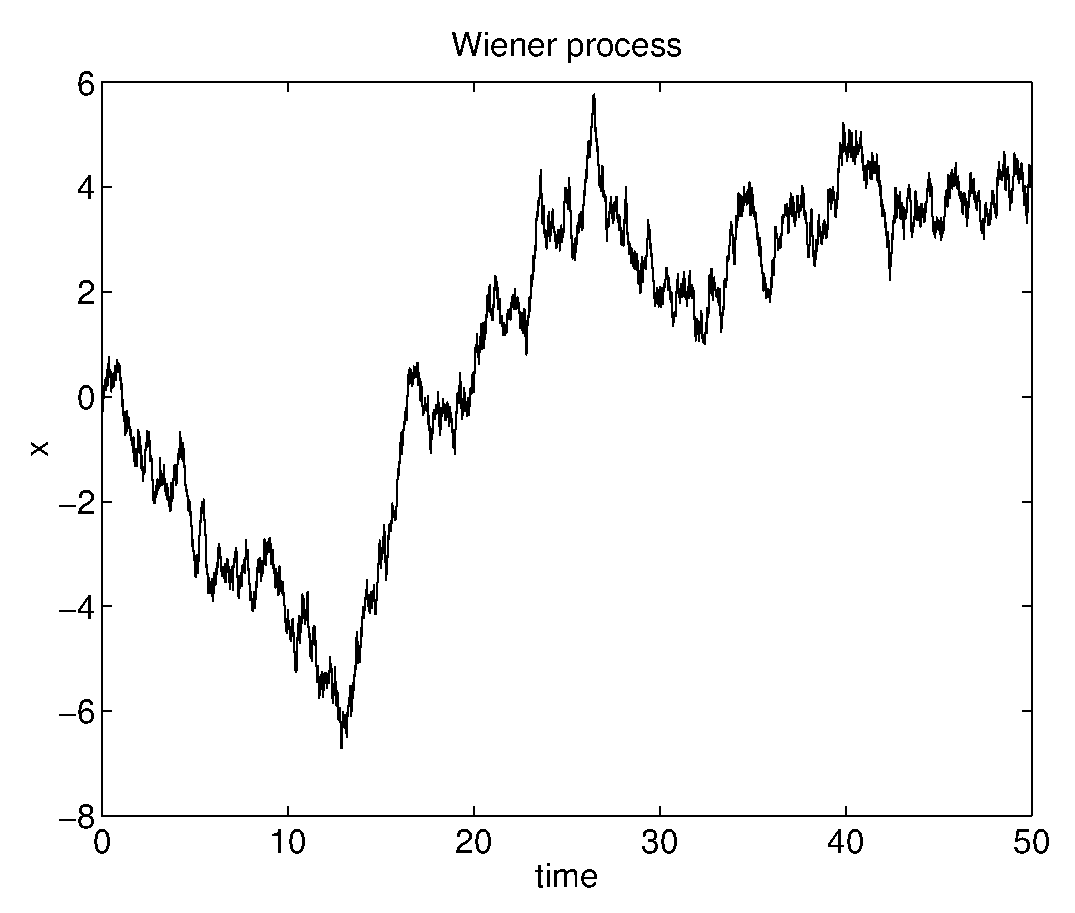
\includegraphics[width=10cm]{./Figures/f_wiener_r1.eps}
\caption{One realization of the Wiener process.
The parameters used in the simulation are \texttt{xstart=0},
\texttt{tend=50}, \texttt{deltat=0.01}, and \texttt{nreal=1}.}
\end{figure}
\begin{figure}
\label{F_WIENER_R2}
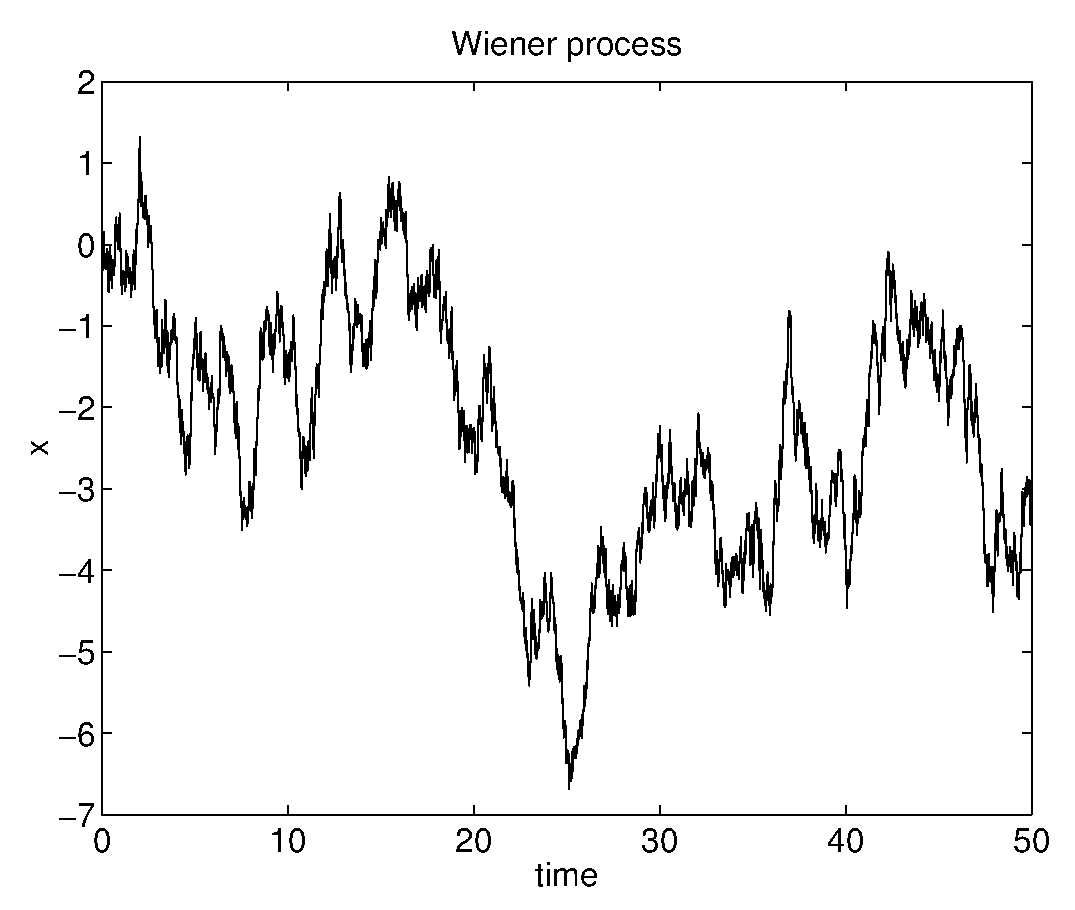
\includegraphics[width=10cm]{./Figures/f_wiener_r2.eps}
\caption{One realization of the Wiener process.
The parameters used in the simulation are \texttt{xstart=0},
\texttt{tend=50}, \texttt{deltat=0.01}, and \texttt{nreal=1}.}
\end{figure}
In Fig. (\ref{F_WIENER}) we show an ensemble average of the
Wiener process over 1000 realizations.
\begin{figure}
\label{F_WIENER}
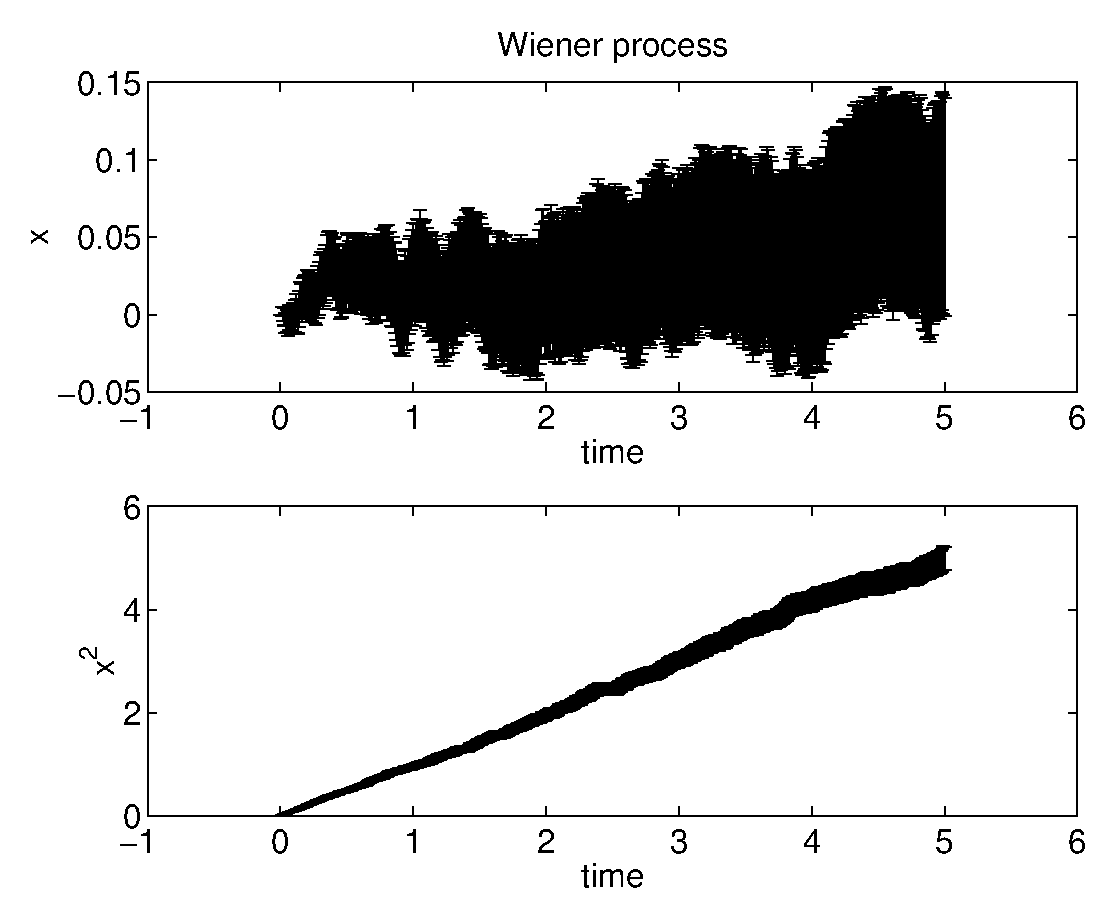
\includegraphics[width=10cm]{./Figures/f_wiener.eps}
\caption{One realization of the Wiener process.
The parameters used in the simulation are \texttt{xstart=0},
\texttt{tend=5}, \texttt{deltat=0.01}, and \texttt{nreal=1000}.}
\end{figure}

\subsection{The Ornstein--Uhlenbeck Process}
Up to now we have considered only Fokker--Planck equations 
without drift. 
As a simple example of a Fokker--Planck equation with an 
additional linear drift we consider
\begin{equation}
\label{ORNSTEIN}
\frac{\partial}{\partial t} T(x,t|x',t') = 
\frac{\partial}{\partial x} [qx T(x,t|x',t')] 
+ \frac{1}{2} D \frac{\partial^2}{\partial x^2} T(x,t|x',t').
\end{equation}
The above Fokker--Planck equation defines the Ornstein--Uhlenbeck
process. 

Again, we can look at the equation of motion for the characteristic
function of the Ornstein--Uhlenbeck process
\begin{equation*}
G(s,t) = \int_{-\infty}^{\infty} dx \exp(isx) T(x,t|x',t').
\end{equation*}
The equation reads
\begin{equation*}
\frac{\partial}{\partial t}G(s,t) = -qs \frac{\partial}{\partial s} 
G(s,t) - \frac{1}{2} Ds^2 G(s,t).
\end{equation*}
The above partial differential equation may be solved by the 
method of characteristics (\cite{gardiner}). Its solution
for $T(x,t_0|x_0,t_0)=\delta(x-x_0)$ requires the
initial condition 
\begin{equation*}
G(s,0) = \exp(ix_0s)
\end{equation*}
and reads
\begin{equation*}
G(s,t) = \exp\left[ -\frac{Ds^2}{4q}[1-\exp(-2q(t-t_0))] + 
 isx'\exp(-q(t-t_0)) 
\right].
\end{equation*}
Hence, the transition probability $T(x,t|x',0)$ is a Gaussian
with mean
\begin{equation}
\label{MEAN_ORNSTEIN}
\langle X(t) \rangle = x_0\exp(-q(t-t_0))
\end{equation}
and variance
\begin{equation}
\label{VAR_ORNSTEIN}
\text{Var} \{ X(t) \} = \frac{D}{2q} [1- \exp(-2q(t-t_0))].
\end{equation}
Since the Ornstein--Uhlenbeck process is a Gaussian process we can write
\begin{equation*}
X(t) = {\bf N}(X_0\exp(-2q(t-t_0)), 
     \frac{D}{2q} (1-\exp(-2q(t-t_0)) ).
\end{equation*}
In contrast to the Wiener process the Ornstein--Uhlenbeck process
has a stationary distribution in the limit $t\longrightarrow \infty$
which is a Gaussian with zero mean and variance $D/2q$.



We now turn to the numerical simulation of realizations of the 
Ornstein--Uhlenbeck process. The problem is to find a way of
determining  from the value of the process $X$ at time $t$
its value at a later time $t+\Delta t$. As for the generation of 
trajectories of the Wiener process it is possible to construct
an update formula for the Ornstein--Uhlenbeck process which is 
exact for any positive value of the time increment $\Delta t$
(\cite{GILLESPIE96}). In order to derive an update formula we
replace in Eqs. (\ref{MEAN_ORNSTEIN}) and (\ref{VAR_ORNSTEIN})
for the mean and variance of the Ornstein--Uhlenbeck process
$t$ by $t+\Delta t$ and $t_0$ by $t$ and accordingly $x_0$ by
$X(t)$. Since we know that the Ornstein--Uhlenbeck process
is Gaussian distributed it is now clear that the update
formula reads
\begin{equation}
X(t+\Delta t) = X(t) \exp(-qt) 
+ \left[ \frac{D}{2q} [1-exp(-2q\Delta t)] \right]^{1/2} \xi,
\end{equation}
where $\xi$ is a Gaussian distributed random number with zero 
mean and unit variance. Since we know how to generate Gaussian 
distributed random numbers the algorithm for the generation of 
realizations of the Ornstein--Uhlenbeck process with diffusion constant
$D$ and inverse relaxation time $q$ reads

(i) Specify the values of $D$, $q$, $x_0$, $\Delta t$.

(ii) Compute the constant coefficients 
\begin{equation*}
\mu \equiv \exp(-q \Delta t)
\end{equation*}
and
\begin{equation*}
\sigma \equiv \left[ \frac{D}{2q} [1-exp(-2q\Delta t)] 
\right]^{1/2}.
\end{equation*}

(iii) Initialize setting $X=x_0$ and $t=0$.

(iv) Replace $t$ by $t+\Delta t$. Terminate the simulation if $t$
exceeed $t_{\text{end}}$.

(v) Generate a Gaussian distributed random number $\xi$ and 
update the process replacing $X$ by $\mu X + \sigma \xi$.

(vi) Goto (iv).

In Fig. (??) we show the flow diagram of the program 
\texttt{ornstein.m} which will be used to generate the 
realizations. The listing of the program can be seen below.

\subsubsection{Listing of the program \texttt{ornstein.m}}
\inputlisting{./Listings/ornstein.m}

One realization of the Ornstein--Uhlenbeck process generated with 
help of the algorithm we have just constructed can be seen in Fig.
(\ref{F_ORNSTEIN_R})

\begin{figure}
\label{F_ORNSTEIN_R}
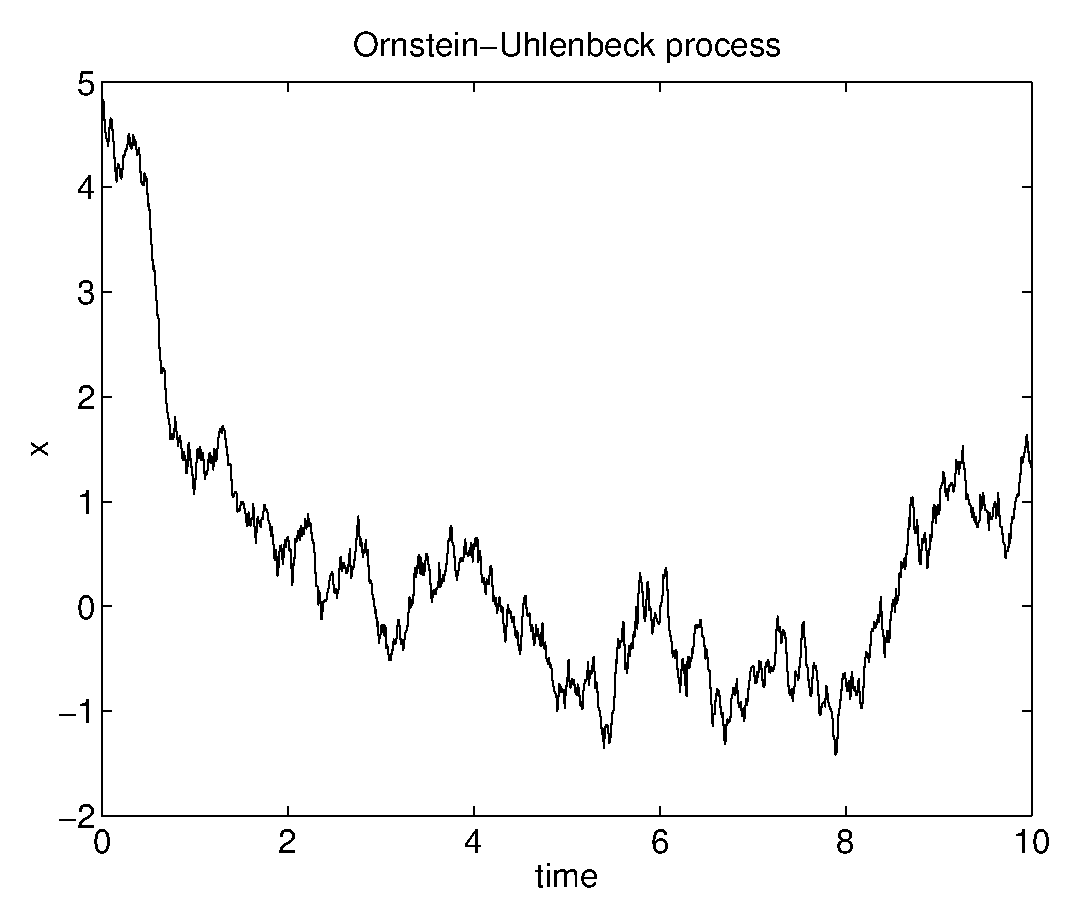
\includegraphics[width=10cm]{./Figures/f_ornstein_r.eps}
\caption{One realization of the Ornstein--Uhlenbeck process. The
 parameters used in the simulation are \texttt{xstart=5},
\texttt{tend=10}, \texttt{deltat=0.01}, \texttt{nreal=1},
\texttt{q=1}, and \texttt{D=1}.}
\end{figure}

The average over 10 realizations of the Ornstein--Uhlenbeck 
process can be seen in Fig. (\ref{F_ORNSTEIN}).
\begin{figure}
\label{F_ORNSTEIN}
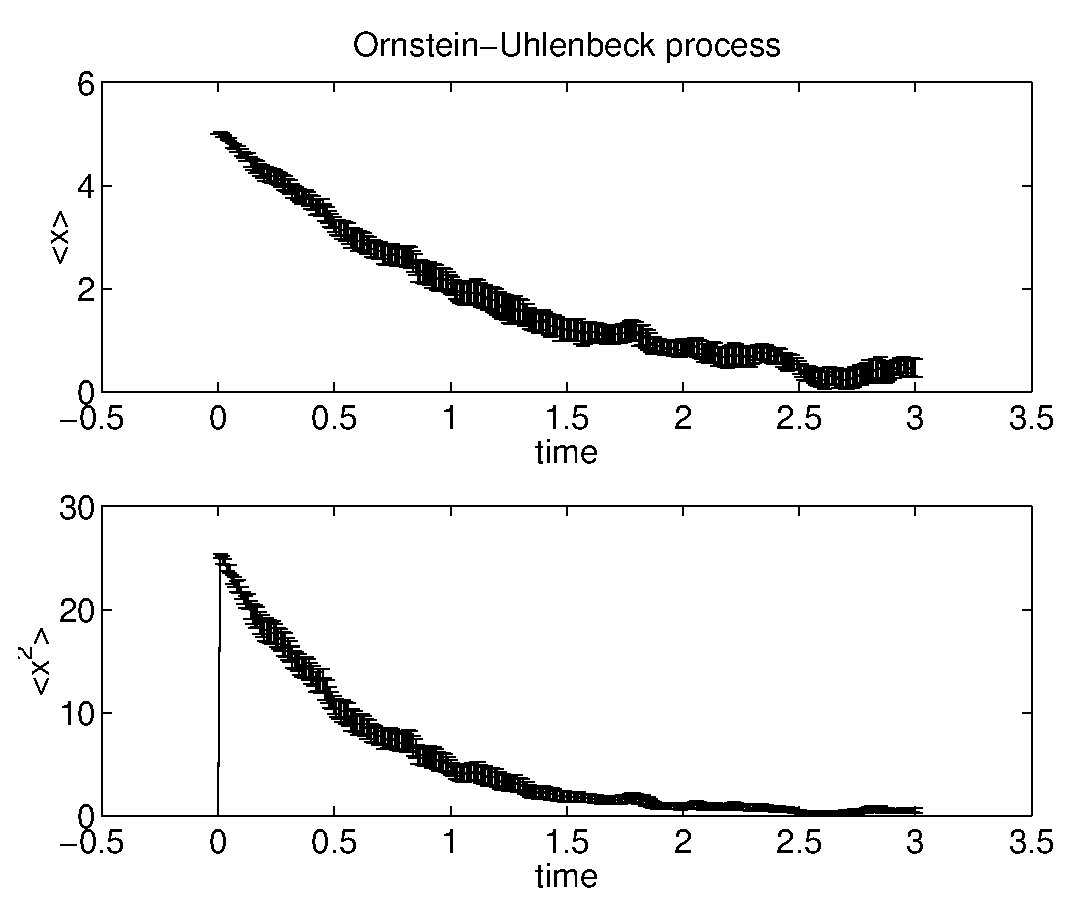
\includegraphics[width=10cm]{./Figures/f_ornstein.eps}
\caption{The average over 10 realizations of the Ornstein--Uhlenbeck 
process. The
 parameters used in the simulation are \texttt{xstart=5},
\texttt{tend=50}, \texttt{deltat=0.01}, \texttt{nreal=10},
\texttt{q=1}, and \texttt{D=1}.}
\end{figure}

%%%%%%%%%%%%%%%%%%%%%%%%%%%%%%%%%%%%%%%%%%%%%%%%%%%%%%%%%%%%%%%%%%%
%%%%%%%%%%%%%%%%%%%%%%%%%%%%%%%%%%%%%%%%%%%%%%%%%%%%%%%%%%%%%%%%%%
\section{Exercises}

\begin{Ex}
\label{Linear_One_Step}
\textbf{Linear one-step process - quantized harmonic oscillator in a %
    radiation field  \cite[page 143]{kampen}} \\
Let $n=0,1,2.\ldots$ numerate the state of a quantized harmonic oscillator 
with energy $h\nu(n+1/2).$ Transitions between the states are induced by the
interaction of the oscillator with the radiation field. The transition 
probability is given by the dipole moments. The only allowed transitions
according to the dipole moments are from $n$ to $n+1$ and from $n$ to $n-1$
(see quantum mechanics lecture).

Therefore the transition rates (probabilities per unit time) are:
\begin{itemize}
\item $g(n-1)=\beta n$ for the transition $(n-1) \rightarrow n$ and
\item $r(n)=\alpha n$ for the transition $n \rightarrow (n-1).$
\end{itemize}
$\alpha$ and $\beta$ are two constants, which depend only on the radiation
density at the frequency $\nu$ and not on $n.$ 

Finally the Master equation for this special one-step process reads
$$ \frac{\partial}{\partial t} P(n,t) = \alpha n P(n+1,t) +\beta(n+1)P(n-1,t)
     -(\alpha n+\beta(n+1))P(n,t).$$

Write a program to simulate the given Master-equation for the one-step
process using the numerical scheme, learned in the lecture.
Choose the parameters $\alpha$ and $\beta$. The result should be a
plot of $P(n,t)$ for different $n$. Plot also $P(n)$ at large $t$, which 
gives the distribution of the
harmonic oscillators with $n$ (and therefore the energy) in the steady state.

The exact stationary solution of the Master-equation
is $P_S(n)= \text{const} \cdot \left(\frac{\beta}{\alpha}\right)^n.$ 
\end{Ex}

\begin{Ex}
\label{Nonlinear_One_Step}
\textbf{Non-linear one-step process - growth of a competitive %
    population \cite[page 163]{kampen} } \\
The number of individuals of some species is called $n.$ The death rate for
this population is $\alpha$ and the birth rate (e.g. by fission)
is $\beta.$ $\alpha$ and $\beta$ are fixed and independent of the
age, otherwise it would not be a Markov process. Both rates are per unit time.

This would be still a linear one-step process. So consider an additional
rate: the competition rate between the individuals of the population.
This rate is an additional death rate and is $\gamma(n-1).$

Therefore the transition rates (probabilities per unit time) are:
\begin{itemize}
\item $g(n)=\beta n$ for the transition $n\rightarrow n+1$
\item $r(n)=\alpha n+\gamma n(n-1)$ for the transition $n \rightarrow n-1.$
\end{itemize}
$\alpha$, $\beta$ and $\gamma$ are constants, which do not depend on $n.$

Finally the Master equation for this one-step process reads
$$ \frac{\partial}{\partial t} P(n,t) = (\alpha n+\gamma n(n-1))P(n+1,t) +
     \beta n P(n-1,t) - (\alpha n+\beta n+\gamma n(n-1))P(n,t).$$

Write again a program to simulate the Master equation and again choose suitable
parameters $\alpha, \beta,\gamma.$ View the time dependence of the population $n$
and try to find out the behaviour of the stationary solutions.

The equation for the first moment (so called macroscopic equation) is called
the {\em Malthus-Verhulst equation} and reads
$$ \dot{<n>} = (\beta-\alpha)<n>-\gamma <n>^2.$$
If you neglect the nonlinear term on the right hand side, 
you get {\em Malthus law}. Then
the solution is just an exponential growth of the population. 

The solutions to the nonlinear equation can be calculated and you get
$$ <n>=\frac{\beta-\alpha}{\gamma} \quad\text{and}\quad <n>\equiv 0 ,$$
where the first one is the stable solution (a so called attractor) 
and the second one is unstable.

{\em example parameters:} $\alpha=0.5, \beta=1, \gamma=0.05 .$
\end{Ex}

\begin{Ex}
\label{Random_Telegraph}
\textbf{The Random Telegraph Process \cite[page 77]{gardiner}} \\
The Random-Telegraph process is the most simple Markov-process possible.
It is a discrete process, which has only two possible states, called
$n=0$ and $n=1$. The master-equation reads
\begin{eqnarray}
 \frac{\partial}{\partial t} P(0,t\mid n'') &= bP(1,t\mid n'')-aP(0,t\mid n'') \\
 \frac{\partial}{\partial t} P(1,t\mid n'') &= aP(0,t\mid n'')-bP(1,t\mid n''). \\
\end{eqnarray}
$a$ and $b$ are the transition rates from state $0\rightarrow 1$
and $1\rightarrow 0$. Examples of this equation are processes, which jump
from one state to the other and back (e.g. spin flipping). 

We can rewrite the two above equations into one equation, resulting in 
the familiar master-equation - DO IT. (you have to ????)
Then write a program to
simulate the master-equation. Use $n=1$ as the initial condition.
For the long time behavior - the stationary solution - the initial
condition is not significant. Try different settings for 
the parameters $a$ and $b$.

Compare the results of the simulation with the exact analytical results.
For $t\to\infty$ the stationary solution for the first moment is:
$$ P(0)=\frac{b}{a+b}, \quad P(1)=\frac{a}{a+b} ,$$  
and
$$ <n> = \sum_{n=0}^1 nP(n)=P(1)=\frac{a}{a+b} .$$
And for the stationary covariance (for the second moment set $t=t'$) 
we get $(t\ge t')$
$$ <n(t)n(t')> = \left(\frac{a}{a+b}\right)^2+\frac{ab}{(a+b)^2}
        e^{-(a+b)(t-t')} .$$

{\em Comment:} This is an example of an ergodic process (a process with
identical ensemble mean and time mean), where you can 
explicitly prove the ergodicity. 
Because if the correlation time is finite, the
system is ergodic. And in this case the correlation time is
$$t_C := \frac{1}{\text{var}(n(0))}\int_0^\infty dt |\text{var}(n(t))| = 
              \frac{1}{(a+b)}$$ 
and therefore finite.
\end{Ex}

\begin{Ex}
\label{Monomolecular_Reaction}
\textbf{Monomolecular Chemical Reaction $A \leftrightarrows X$  %
       \cite[page 183]{schnakenberg} } \\
A further example of a discrete one-step process is a chemical reaction,
where an atom can be either bound to a molecule (call it state X) 
or be by itself (call it state A). We assume that we have an A-reservoir,
so that there are always enough atoms to become absorbed by a molecule. 
The number of molecules (state X) is called $N$, the number of atoms $A.$ 
Another example of
this situation would be an atom in the ground state at a given temperature.
The atom jumps to a higher state and back, depending on the temperature;
assuming low temperatures (A-reservoir).

For chemical reactions the transition rates are given by the rate-constant
$k$, depending on the temperature. The derivation is based on the 
Sto�zahlansatz. So the transition of atoms to molecules is proportional
to the number of atoms in the reservoir $A$ and the transition of molecules
releasing an atom is proportional to the number of molecules $N.$
$$ W_{N+1,N} = A \quad \text{and} \quad W_{N-1,N} = kN .$$

Then the master-equation is
$$ \frac{\partial}{\partial t} P(N,t) = AP(N-1,t)+k(N+1)P(N+1,t)-(A+kN)P(N,t).$$

Again write a program to simulate the master-equation. Use $k=1, A=100$ for
the parameters and $N(0)=A$ as initial value.
Then compare the simulation results with the analytical results:
$$ <N(t)> = A+ (<N(0)>-A)e^{-t} \longrightarrow A \quad\text{for}\quad 
                 t\to\infty,$$
$$ P_{\text{stat}}(N) = \frac{A^N}{N!} e^{-kA} \qquad 
          \text{Poisson-distribution} . $$ 
Also try different parameters and initial conditions.

{\em Comment:} In this example we assumed that there is enough time for the 
reactants to diffuse in the volume. That means the diffusion of atoms and 
molecules is very fast compared to the time a reaction takes place.
If the two time scales are almost the same, we also have to simulate
the diffusion. Such systems are known as reaction-diffusion systems
- we will discuss them later on.
\end{Ex}

\begin{Ex}
\label{Payroll}

\end{Ex}

%%%%%%%%%%%%%%%%%%%%%%%%%%%%%%%%%%%%%%%%%%%%%%%%%%%%%%%%%%%%%%%%%%%%%


\bibliographystyle{peter}
\bibliography{V_98,simulit}

%%%%%%%%%%%%%%%%%%%%%%%%%%%%%%%%%%%%%%%%%%%%%%%%%%%%%%%%%%%%%%%%%%
%%%%%%%% Ende von Kap. 4 %%%%%%%%%%%%%%%%%%%%
%%%%%%%%%%%%%%%%%%%%%%%%%%%%%%%%%%%%%%%%%%%%%%%%%%%%%%%%%%%%%%%%%%%%%


%%% Chapter 5 

\chapter{Stochastic Differential Equations}

In the previous section we have derived an exact simulation algorithm
for the generation of trajectories of the Ornstein--Uhlenbeck process.
The ``exact'' update formula was
\begin{equation*}
X(t+\Delta t) = X(t) \exp(-q \Delta t) +
  \left[ \frac{D}{2q}(1-\exp(-2q\Delta t)) \right]^{1/2} \xi(t),
\end{equation*}
where we have now written $\xi(t)$ to stress the fact that at each
time step $t$ we have to draw another Gaussian distributed random 
number. The update formula is exact in the sense that it holds for
arbitrary values of $\Delta t$.

However, it will turn out to be convenient to have an update formula
which works for small values of $\Delta t$. To this end we expand the
exact update formula to first order in $\Delta t$ and obtain
\begin{eqnarray}
X(t+\Delta t)& =& X(t) (1- q \Delta t) + 
   \left[ \frac{D}{2q} (2q \Delta t) \right]^{1/2} \xi(t) \nonumber
   \\
\label{SDE_APPROX} 
  & = & X(t) - qX(t) \Delta t + \sqrt{D} \sqrt{\Delta t} \xi(t).
\end{eqnarray}
In the limit $\Delta t \rightarrow 0$ this approximate update formula
turns exact.  We recognize immediately that the stochastic increment in
this discretized version of the Ornstein--Uhlenbeck process scales
with the square root of the time increment $\Delta t$.

Note that in deriving the above discretized update formula we have 
intentionally omitted the terms linear in $\Delta t$ stemming from 
the expansion of the factor in front of the stochastic term. In 
doing so we have achieved that the update formula has an important
property. Namely, it is selfconsistent in the following sense
(\cite{GILLESPIE}). Let us apply the above formula twice, starting from,
\begin{equation*}
X(t+2\Delta t) = X(t+\Delta t) 
 - qX(t+ \Delta t) \Delta t + \sqrt{D} \sqrt{\Delta t} \xi(t+\Delta t).
\end{equation*}
Inserting (\ref{SDE_APPROX}) we immediately obtain keeping 
terms up to first order in $\Delta t$
\begin{equation*}
X(t+2 \Delta t) = X(t) - q X(t) 2 \Delta t +
   \sqrt{D} \sqrt{\Delta t} [\xi(t) + \xi(t+\Delta t)].
\end{equation*}
Since $\xi(t)$ and $\xi(t+\Delta)$ are statistically independent
Gaussian stochastic processes we have
\begin{equation*}
\xi(t) + \xi(t+\Delta t) = {\bf N}(0,1) + {\bf N}(0,1) =
  {\bf N}(0,2) = \sqrt{2} {\bf N}(0,1),
\end{equation*}
so that we finally have
\begin{equation*}
X(t+2 \Delta t) = X(t) - q X(t) 2 \Delta t +
   \sqrt{D} \sqrt{2 \Delta t} \xi(t).
\end{equation*}
This selfconsistency of the discretized stochastic differential 
equation expresses essentially the fundamental properties
of the propagator of a Markov process as they are defined in
the Chapman--Kolmogorov equation.


Due to the presence of a stochastic term, the Gaussain stochastic
process $\xi(t)$, the above equation is a discretized version of a 
so--called {\em stochastic differential equation} (SDE). It is the aim
of this section to introduce into some  peculiarities of stochastic
differential equations. In particular we will also show the
equivalence of stochastic processes defined in terms of stochastic differential
equations and in terms of Fokker--Planck equations.

The above expression is a special case of the  {\em standard form} of
a stochastic differential equation (some times stochastic
differential equations are also called {\em Langevin} equations):
\begin{equation}
\label{SDE_LANGEVIN_DISCR}
X(t+dt) = X(t) + A(X(t),t)dt + \sqrt{D(X(t),t)} \xi(t) dt^{1/2},
\end{equation}
where we have replaced $\Delta t$  by $dt$ to stress the infinitesimal
character of the above equation. The term proportional to $dt$ is
called the {\em drift term}, whereas the term proportional to
$\sqrt{dt}$ is called the diffusion term. 

The above definition of the stochastic process $X(t)$
in terms of a stochastic differential equation  cleary shows that
the stochastic process $X(t)$ is continuous, but, in general, not 
differentiable. This can be seen by writing
Eq. (\ref{SDE_LANGEVIN_DISCR}) as
\begin{equation*}
\label{eq:XiinSDE}
\frac{X(t+dt) - X(t)}{dt} = A(X(t),t) + \frac{\sqrt{D(X(t),t)} \xi(t)}
                                              {\sqrt{dt}}.
\end{equation*}
Obviously, the limit $dt \rightarrow 0$ of the above equation does not
exist, unless $D\equiv 0$. Thus, a purely stochastic Markov process
is everywhere continuous but nowhere differentiable. Nevertheless it is
customary in the physical literature to ``pretend'' (\cite{GILLESPIE})
that $dx/dt$ exists even for
non vanishing $D$. In fact we know that we can write (see section
\ref{sec:WienerProcess})
\begin{equation*}
\frac{\xi(t)}{\sqrt{dt}} = \frac{1}{\sqrt{dt}} {\bf N}(0,1) =
{\bf N}(0,1/dt).
\end{equation*}
So, we may define a Gaussian {\em white noise process} as
\begin{equation*}
\eta(t) \equiv \lim_{dt \rightarrow 0}  {\bf N}(0,1/dt).
\end{equation*}
With the help of the above definition, we can now formally write
(compare with \ref{eq:XiinSDE})
\begin{equation*}
\frac{d}{dt} X(t) = A(X(t),t) + \sqrt{D(X(t),t)} \eta(t).
\end{equation*}
This equation is called the white noise form of the Langevin equation.
The white noise process introduced above does have the following
averaged properties:
\begin{eqnarray*}
\langle \eta(t) \rangle &=& 0 \\
\langle \eta(t) \eta(t') \rangle &=& \delta(t-t'),
\end{eqnarray*}
which satisfy the requirement of no correlation at different
times. Note, that the white noise process  $\eta$ has
infinite variance. Accordingly, the spectral density, i.e.,
the Fourier transform of the correlation function of $\eta$ is 
constant. This is the reason for calling $\eta$ a white noise
process.

It is important to establish precisely the relationship
between the white noise process and the Wiener process
(\cite{GILLESPIE}).
We know already that the special Wiener process $dW(dt)$
is a normal random variable with mean zero and variance $dt$
\begin{equation*}
dW(dt) = {\bf N}(0,dt).
\end{equation*}
It follows from the theorems of Gaussian probability densities
that
\begin{equation*}
{\bf N}(0,dt) =  dt {\bf N}(0,1/dt).
\end{equation*}
Because of the definition of the Gaussian white noise process we 
can conclude that
\begin{equation*}
dt \eta(t) = dW(dt)
\end{equation*}
and hence we have formally in the limit $dt \rightarrow 0$
\begin{equation*}
\frac{dW}{dt} = \eta(t).
\end{equation*}
This equation asserts that the derivative of the Wiener process is 
the white noise process. However, we know already that the Wiener
process is not differentiable so that the white noise process must 
be ill--defined. We will see shortly how these formal difficulties 
may easily be circumvented in the proper definition
of stochastic differential equations. Before doing so we will 
consider for a 
moment the most classical Langevin equation of statistical 
physics, namely the one describing Brownian motion.

\section{The Langevin Equation and Brownian Motion}
In 1908 Langevin considered the problem of the dynamical 
description of Brownian motion (\cite{VAN_KAMPEN}). 
He suggested that the equation of 
motion of a Brownian particle with mass $m=1$ be described by the
following differential equation for the velocity $V$
\begin{equation}
\label{LANGEVIN}
\frac{d}{dt} V = -\gamma V + L(t),
\end{equation}
where the terms on the right hand--side of the above equation 
model the forces which the surrounding molecules excerpt on the 
Brownian particle. Since these forces are unknown in detail the 
following assumptions were postulated. The Brownian particle 
moving in the fluid of surrounding particles feels
a dissipative drag force which is proportional to its velocity, $\gamma$  being 
the friction coefficient. Furthermore, the Brownian particle hits
the surrounding particles. These collisions cause irregular 
changes in the velocity of the Brownian particle. Thus, the external force
$L(t)$ is modeled as a zero mean, temporally uncorrelated
randomly fluctuating force. The first two moments of the
stochastic process $L(t)$ are assumed to 
have the following properties
\begin{eqnarray*}
\langle L(t) \rangle &=& 0 \\
\langle L(t) L(t') \rangle &=& \Gamma \delta(t-t').
\end{eqnarray*}

The Langevin equation is the prototype of a stochastic 
differential equation, i.e. of a differential equation whose
coefficients are random functions of the time with some given
statistical properties. 
It is clear that choosing $L(t)=\sqrt{\Gamma} \eta(t)$,
where $\eta(t)$ is a Gaussian white noise process, the Langevin 
equation of Brownian motion describes an Ornstein--Uhlenbeck
process.
The stochastic process $V(t)$ is 
completely defined once an initial condition $V(0)=V_0$ is specified.
Its formal solution reads
\begin{equation*}
V(t) = V_0 \exp(-\gamma t) + \exp(-\gamma t) 
    \int_0^t dt' \exp(\gamma t') L(t').
\end{equation*}
Taking the average over an ensemble of Brownian particles all
having the same initial condition we find for the mean value of 
the velocity
\begin{equation*}
\langle V(t) \rangle = V_0 \exp(-\gamma t),
\end{equation*}
where we made use of the statistical properties of the Langevin 
force $L(t)$. Accordingly, the second moment of the velocity field
is found to be
\begin{eqnarray*}
\langle V^2(t) \rangle &=& V_0^2 \exp(-2\gamma t)
          + \exp(-2 \gamma t) \int_0^t dt'' \int_0^t dt'
             \exp(\gamma (t' + t'')) \langle L(t') L(t'') \rangle 
             \\
          &=& V_0^2 \exp(-2\gamma t) + \frac{\Gamma}{2 \gamma}
             [1-\exp(-2 \gamma t)].
\end{eqnarray*}
Up to now the constant $\Gamma$ was left unspecified. From 
equilibrium statistical physics (theorem of equipartition of energy) 
we  expect that for long times 
\begin{equation*}
\langle V^2(t\rightarrow \infty) \rangle = kT.
\end{equation*}
Hence we have
\begin{equation}
\label{FDT1}
\Gamma = 2 \gamma kT
\end{equation}
and we have established a relation between the attrition 
coefficient $\gamma$ and the random fluctuations.
Eq. (\ref{FDT1}) is a simple version of the so--called
fluctuation--dissipation theorem.


\section{Stochastic Integration}
It is the aim of this section to show how the formal problems
arising in the formulation of Langevin equations can be avoided.
Let us begin by formulating the Langevin equation in a discrete 
way,
\begin{equation*}
dX(t) = a(X(t),t) dt + b(X(t),t) \eta(t) dt,
\end{equation*}
where $a(X(t),t)$ is a deterministic drift and $b(X(t),t)$ is the 
diffusion term, $\eta(t)$ being a Gaussian white noise process.
We proceed by integrating the above equation from $t_0$ to $t$
and obtain for each sample path
\begin{equation*}
X(t) = X(t_0) + \int_{t_0}^t ds a(X(s),s) 
+ \int_{t_0}^t b(x(s),s) \eta(s) ds.
\end{equation*}
Since the Wiener process $W(t)$ can be represented as the integral
over a white noise process, i.e.,
\begin{equation}
W(t) = \int_{t_0}^t ds \eta(s)
\end{equation}
the integral form of the Langevin equation can be written as
\begin{equation}
\label{SDE_INTEGRAL}
X(t) = X(t_0) + \int_{t_0}^t ds a(X(s),s) 
+ \int_{t_0}^t b(x(s),s) dW(s).
\end{equation}
The above expression is 
expected to make sense because the Wiener process is continuous. 
We will see shortly that the above 
equation does have a precise meaning. In fact
from here on a solution of a stochastic differential equation will be 
interpreted as a solution 
of the corresponding integral equation, which will be written
in the short--hand notation
\begin{equation*}
dX(t) =   a(X(t),t) dt + b(x(t),t) dW(t).
\end{equation*}

Of course, the second integral in Eq. (\ref{SDE_INTEGRAL}) is not 
an ordinary integral.  It is an integral with respect to the 
Wiener process $W(t)$. Such integrals are called {\em stochastic 
integrals} and we will define and discuss them now. For a precise
mathematical definition of stochastic integrals see \cite{GARD, 
POTTER,KLOEDEN_AN,OETTINGER}. We will follow here the more
{\em physical} line of reasoning of \cite{gardiner}.

\subsection{Definition of the Stochastic Ito Integral}
The starting point for the definition of the Ito integral is the
following reasoning. For $b(X(t),t)=b=\text{const}$, the stochastic 
integral
\begin{equation*}
I = \int_{t_0}^t bdW(s)
\end{equation*}
is expected to be defined and to be equal to
\begin{equation*}
I = b \{ W(t) - W(t_0) \}.
\end{equation*}
In general it seems to be safe to treat the stochastic 
integral 
\begin{equation*}
I(f) = \int_{t_0}^t f(X(s),s) dW(s)
\end{equation*}
as a kind of Riemann--Stieltjes integral, i.e., as a limit of 
partial sums. To do so we divide the interval $[t_0,t]$ into $n$
subintervals
\begin{equation*}
t_0 \le t_1 \le t_2 \le \cdots \le t_{n-1} \le t_n \equiv t
\end{equation*}
and define intermediate points $\tau_i$
\begin{equation*}
t_{i-1} \le \tau_i \le t_i.
\end{equation*}
The stochastic integral $I(f)$ is then defined as the limit
of the partial sums
\begin{equation*}
S_n = \sum_{i=1}^n f(\tau_i) \left[  W(t_i) - W(t_{i-1}) \right].
\end{equation*}
In general it turns out that the definition of the stochastic 
integral depends on the particular choice of the intermediate 
point $\tau_i$. In the definition of the Ito stochastic integral
the intermediate points are chosen to be at the beginning of
the corresponding time interval, i.e.,
\begin{equation*}
\tau_i = t_{i-1}.
\end{equation*}
Accordingly the Ito stochastic integral is defined as the limit of 
the partial sums
\begin{equation*}
S_n = \sum_{i=1}^n f(t_{i-1}) [  W(t_i) - W(t_{i-1}) ].
\end{equation*}
The limit of the sequence of partial sums is to be understood in the
following sense. The random variable $S_n$ is said to converge to $S$
 in the mean square limit if
\begin{equation*}
\lim_{n \rightarrow \infty}
 <(S_n -S)^2> =0.
\end{equation*}
The above limit is usually written as
\begin{equation*}
\text{ms-} \lim_{n \rightarrow \infty} S_n = S.
\end{equation*}
In this sense the Ito stochastic integral of the function $f(t)$ is
defined as
\begin{equation*}
\int_{t_0}^t f(x(t'),t') dW(t') = \text{ms-}\lim_{n \rightarrow \infty}
   \left\{ \sum_{i=1}^{n} f(t_{i-1}) [W(t_i) - W(t_{i-1})] 
   \right\}.
\end{equation*}

\subsection{The Stratonovich Stochastic Integral}
\label{STRATONOVICHSUB}
An alternative definition of a stochastic  integral has been given by
Stratonovich. He suggested the following definition
\begin{equation}
\label{STRATONOVICHDEFI}
S\int_{t_0}^t f(x(t'),t') dW(t') = \text{ms-}\lim_{n \rightarrow \infty}
   \left\{ \sum_{i=1}^{n} f( \frac{x(t_{i})+ x(t_{i-1})}{2}, t_{i-1}) 
[W(t_i) - W(t_{i-1})]   \right\}.
\end{equation}
The $S$ in front of the integral denotes a Stratonovich integral
in contrast to the Ito integral.
Note, that in this definition the integrand is evaluated in an
averaged way.

\subsection{Ito Calculus}
We now want to derive some very useful formulas. In order to do so 
we have to introduce a special class of functions. A function $g(t)$
is called a {\em nonanticipating function} of $t$ if for all
$s$ and $t$ such that $t<s$, $g(t)$ is statistically independent 
of $W(s)-W(t)$. In other words $g(t)$ is independent of the 
behaviour of the Wiener process in the future of $t$. Within the 
context of the stochastic differential equations such functions 
are quite reasonable since they express the fact that the future 
does not affect the present. This guarantees, evidently, 
causality.

We are now in the position to give the proof of the fundamental 
equation of Ito calculus, namely, that
\begin{equation*}
dW(t)^2 = dt 
\end{equation*}
and that
\begin{equation*}
dW(t)^{2+N} =0 
\end{equation*}
for $N \ge 1$. These formulas will allow for a comfortable 
handling of stochastic differentials.

We begin by proofing that
\begin{equation}
\label{PROOFDW2DT}
\int_{t_0}^t \left[ dW(t') \right]^2 g(t') = \int_{t_0}^t dt' 
g(t')
\end{equation}
for a nonanticipating function $g(t)$. By definition of the 
stochastic Ito integral we have
\begin{eqnarray*}
\int_{t_0}^t \left[ dW(t') \right]^2 g(t') & = & 
\text{ms-}\lim_{n \rightarrow \infty} \sum_i g_{i-1} \Delta W_i^2 \\
   & = & \lim_{n \rightarrow \infty} 
    < \left[ \sum_i g_{i-1} \Delta W_i^2 \right]^2>.
\end{eqnarray*}
Eq. (\ref{PROOFDW2DT}) is of course to be understood in the mean
square sense, so we consider the following expression
\begin{eqnarray*}
I & = & \lim_{n \rightarrow \infty} 
< \left[ \sum_i g_{i-1} (\Delta W_i^2  -\Delta t_i)\right]^2   > 
\\
& = & \lim_{n \rightarrow \infty} 
<  \sum_i (g_{i-1})^2 (\Delta W_i^2  -\Delta t_i^2)
+\sum_{i>j} 2 g_{i-1}g_{j-1} (\Delta W_j^2  -\Delta t_j)
 (\Delta W_i^2  -\Delta t_i) >.
\end{eqnarray*}
We can now exploit the fact that in the first sum in the above expression
the $(g_{i-1})^2$ and $(\Delta W_i^2  -\Delta t_i^2)$ and accordingly in the 
second sum $g_{i-1}g_{j-1} (\Delta W_j^2  -\Delta t_j)$ and 
$(\Delta W_i^2  -\Delta t_i)$ are statistically independent from 
each other because the function $g$ is nonanticipating and because 
of the properties of the Wiener process. This statistical 
independence permits to factorize the mean value. So we find
\begin{equation*}
I = 2 \lim_{n \rightarrow \infty} 
\left[ \sum_i \Delta t_i <(g_{i-1})^2> \right],
\end{equation*}
where we have used the following properties of the Wiener process
\begin{equation*}
<\Delta W_i^2> = \Delta t_i
\end{equation*}
and
\begin{equation*}
<(\Delta W_i^2 - \Delta t_i)^2> = 2 \Delta t_i^2.
\end{equation*}
Hence we can conclude that
\begin{equation*}
\text{ms-}\lim_{n \rightarrow} 
\left( \sum_i g_{i-1} \Delta W_i^2 - \sum_i g_{i-1} \Delta t_i \right)
=0.
\end{equation*}
Since 
\begin{equation*}
\text{ms-}\lim_{n\rightarrow \infty} \sum_i g_{i-1} \Delta t_i =
\int_{t_0}^t dt' g(t')
\end{equation*}
we have completed the proof of Eq. (\ref{PROOFDW2DT}).
The importance of Eq. (\ref{PROOFDW2DT}) is the following one. Because
of the definition of stochastic differential equations $dW(t)$
occurs only in integrals, so that we can explicitly write
\begin{equation*}
dW(t)^2 \equiv dt.
\end{equation*}
Accordingly, it is straightforward to show that in the same sense
\begin{equation*}
dW(t)^{2+N} \equiv 0, \;\;\; \text{for} \;\;\; N>0.
\end{equation*}
In the following it will be of some importance to have 
multiplication rules for stochastic differentials. The following
multipication table sums up the rules for products of stochastic 
differntials.
\begin{table}
\caption{Multiplication table for products of stochastic differentials.}
\begin{center}
\begin{tabular}{|c||c|c|c|}\hline 
$\times$ & $dW$ & $dW^2$ & $dt$ \\ \hline \hline
$dW$     & $dt$ & $0$    & $0$   \\ \hline
$dW^2$   &  $0$ & $0$    &  $0$  \\ \hline
$dt$     &  $0$ & $0$    & $0$  \\ \hline
\end{tabular}
\end{center}
\end{table}
As an example of the application of the above formulas we consider the
integration of a polynomial. Let us look at
\begin{eqnarray*}
d[W(t)]^n & = & [W(t) + dW(t)]^n - W(t)^n \\
          & = & \sum_{r=1}^n \binom{n}{r} W(t)^{n-r} dW(t)^r .
\end{eqnarray*}
Using the fact that $dW(t)^r = 0$ for $r>2$ we conclude that
\begin{equation*}
d[W(t)]^n = n W(t)^{n-1}dW(t) +
\frac{n(n-1)}{2} W(t)^{n-2} dt
\end{equation*}
so that
\begin{equation*}
\int_{t_0}^t W(t')^n dW(t') = \frac{1}{n+1}  [W(t)^{n+1} - W(t_0)^{n+1}]
   -\frac{n}{2} \int_{t_0}^t W(t')^{n-1} dt.
\end{equation*}



\section{Ito Stochastic Differential Equations}
Having defined stochastic integrals the proper definition of a
stochastic differential equation can be given (Again we follow 
\cite{gardiner}. The mathematically interested reader should
consult \cite{GARD,KLOEDEN_AN,POTTER}). The stochastic variable
$X(t)$ obeys the Ito stochastic differential equation
\begin{equation}
\label{ITOSDE}
dX(t) = a(X(t),t) dt + b(X(t),t) dW(t)
\end{equation}
if for all $t$ and $t_0$ the following integral equation holds
\begin{equation}
X(t) = X(t_0) + \int_{t_0}^t ds a(X(s),s) 
     + \int_{t_0}^t dW(s) b(X(s),s).
\end{equation}

\subsection{Ito's Formula}
In this subsection we want to consider a function
$f$ of the stochastic variable $X(t)$ and derive an Ito stochastic
differential equation for $f$. We begin by expanding the differential 
$df(x(t))$ to second order in $dW(t)$
\begin{eqnarray*}
df(X(t)) & = & f(X(t)+dX(t)) - f(X(t)) \\
         & = & f'(X(t)) dX(t) + \frac{1}{2} f''(X(t)) dX(t)^2 + \ldots.
\end{eqnarray*}
Inserting the Ito stochastic differential equation (\ref{ITOSDE})
for $dX(t)$ we get
\begin{eqnarray*}
df(X(t)) &=&  f'(X(t)) \{a(X(t),t)dt + b(X(t),t) dW(t) \} \\
      & & + \frac{1}{2} f''(X(t)) b(X(t),t)^2 [dW(t)]^2 + \ldots ,
\end{eqnarray*}
where we have discarded all other terms of higher order. Using
finally $[dW(t)]^2 =dt$ we get
\begin{eqnarray}
\label{ITOFORMULA}
df(X(t)) &=& \{a(X(t),t) f'(X(t)) +  \frac{1}{2} f''(X(t)) b(X(t),t)^2
\} dt  \nonumber \\
    & & + b(X(t),t)f'(X(t)) dW(t).
\end{eqnarray}
The above equation is Ito's formula and expresses the fact that 
in general for stochastic differential equations
the change of variables is not given by the rules of 
ordinary calculus.


\subsection{The Equivalence of Stochastic Differential Equations 
  and of the Fokker--Planck Equation}
Let us now look at the time development of the expectation value 
of an arbitrary function
$f(X(t))$.
Using Ito's formula we immediately have
\begin{eqnarray*}
\frac{<df(X(t))>}{dt} & = & \left< \frac{df(X(t))}{dt} \right> = 
               \frac{d}{dt} <f(X(t)) > \\
       & = & < a(X(t),t) f'(X(t)) +   \frac{1}{2} f''(X(t)) b(X(t),t)^2   >.
\end{eqnarray*} 
Since, $X(t)$ is a Markov process it does have a conditional
probability density $T(x,t|x_0,t_0)$ and accordingly we can write
\begin{eqnarray*}
\frac{d}{dt} <f(X(t)) > &=& \int dx f(x) \frac{\partial}{\partial t} 
         T(x,t|x_0,t_0) \\
          & = & \int dx 
       [a(X(t),t) f'(X(t)) +   \frac{1}{2} f''(X(t)) b(X(t),t)^2] T(x,t|x_0,t_0).
\end{eqnarray*}
The above equation can now be integrated by parts. Disregarding
surface terms we obtain
\begin{equation*}
\int dx f(x) \frac{\partial}{\partial t} T = \int dx f(x)
   \{ - \frac{\partial}{\partial x}[a(x,t)T] + \frac{1}{2} 
        \frac{\partial^2}{\partial x^2}[b(x,t)^2 T] \}.
\end{equation*}
Since, by construction $f$ is an arbitrary function of $x$ we can
conclude that
\begin{equation*}
 \frac{\partial}{\partial t} T(x,t|x_0,t_0) =
    - \frac{\partial}{\partial x}[a(x,t)T(x,t|x_0,t_0)] + \frac{1}{2} 
        \frac{\partial^2}{\partial x^2}[b(x,t)^2 T(x,t|x_0,t_0)].
\end{equation*}
We immediately recognize that the above equation is a Fokker--Planck
equation. Hence we have shown the equivalence of a diffusion
process defined in terms of a stochastic differential equation with
drift coefficient $a(x(t),t)$ and a diffusion coefficient
$b(X(t),t)^2$ and the above Fokker--Planck equation.

\section{The Stratonovich Stochastic Differential Equation}
In subsection \ref{STRATONOVICHSUB} we have seen that it is 
possible to give other definitions of the stochastic integral.
One such definition is the Stratonovich stochastic integral defined 
in Eq. (\ref{STRATONOVICHDEFI}). It is clear that it is then possible 
to define stochastic differential equations using the 
Stratonovich integral, i.e.,
\begin{equation}
\label{STRATOSDE}
X(t) = X(t_0) + \int_{t_0}^t ds \alpha(x(s),s) +
      S \int_{t_0}^t dW(s) \beta(x(s),s).
\end{equation}
In the mathematical literature it is customary to write
the Stratonovich integral in the form
\begin{equation*}
\int_{t_0}^t  \beta(x(s),s) \circ dW(s) 
\equiv S\int_{t_0}^t  \beta(x(s),s) dW(s) ,
\end{equation*}
where the notation $\circ$ is called the {\em Ito circle}. From
here on we will also stick to this notation.
It is the aim of this subsection to show that stochastic 
differential equations defined in terms of the Stratonovich 
integral are equivalent to some appropriate Ito stochastic 
differential equations.

To this end we assume that the above $x(t)$ is also a solution of the Ito 
stochastic differential equation
\begin{equation}
\label{ITOSDEINS}
dx(t) = a(x(t),t) dt + b(x(t),t) dW(t)
\end{equation}
and try to derive expressions for the corresponding $\alpha$ and $\beta$
in Eq. (\ref{STRATOSDE}).

We begin by establishing the relation between the Ito and the 
Stratonovich integral. By definition of the Stratonovich integral 
we have
\begin{equation}
\label{STRATOIAPP}
\int_{t_0}^t  \beta(x(s),s) \circ dW(s) \approx
 \sum_i \beta \left( \frac{x(t_i) + x(t_{i-1})}{2},t_{i-1} \right)
  [W(t_i) -W(t_{i-1})].
\end{equation}
Using
\begin{equation*}
x(t_i) = x(t_{i-1}) + dx(t_{i-1})
\end{equation*}
the argument of the $\beta$ function can be written as
\begin{equation*}
\beta \left( \frac{x(t_i) + x(t_{i-1})}{2},t_{i-1} \right) =
 \beta \left( x(t_{i-1}) + \frac{1}{2} dx(t_{i-1}) ,t_{i-1}\right).
\end{equation*}
Then, with the help of the Ito stochastic differential equation 
(\ref{ITOSDEINS}) in the form
\begin{equation*}
dx(t_i) = a(x(t_{i-1}),t_{i-1}) (t_i -t_{i-1}) + 
   b(x(t_{i-1}),t_{i-1}) (W(t_i) -W(t_{i-1}))
\end{equation*}
and of Ito's formula we get
\begin{eqnarray*}
\beta \left( \frac{x(t_i) + x(t_{i-1})}{2},t_{i-1} \right) & = &
 \beta(t_{i-1}) + \left[ a(t_{i-1}) \frac{\partial}{\partial x} 
 \beta(t_{i-1}) + \frac{1}{4} b^2(t_{i-1})
                  \right] \frac{1}{2}(t_{i} - t_{i-1}) \\
 &  + & \frac{1}{2} b(t_{i-1}) \frac{\partial}{\partial x} 
 \beta(t_{i-1}) [W(t_i) - W(t_{i-1})].
\end{eqnarray*}
The above expression can now be inserted back into the Eq. 
(\ref{STRATOIAPP}). Exploiting the fact that Ito calculus allows us to set 
$dW^2=dt$ and to drop the terms $dt^2$ and $dtdW$ we find
\begin{eqnarray*}
\int_{t_0}^t  \beta(x(s),s) \circ dW(s) & \approx &
\sum_i \beta(x(t_{i-1}),t_{i-1}) [W(t_i) - W(t_{i-1})] \\
 &  + & \frac{1}{2} \sum_i b(x(t_{i-1}),t_{i-1}) 
 \frac{\partial}{\partial x} \beta(x(t_{i-1}),t_{i-1}) (t_i - 
 t_{i-1}).
\end{eqnarray*}
Since the first term on the right side of the above equation is a
partial sum of an Ito integral we conclude from the above discrete
formula that
\begin{equation}
\int_{t_0}^t  \beta(x(s),s) \circ dW(s) = 
\int  \beta(x(t'),t') dW(t') 
 + \frac{1}{2} \int b(x(t'),t') 
 \frac{\partial}{\partial x} \beta(x(t'),t') dt'.
\end{equation}
The above formula gives us the relation between the Ito and the 
Stratonovich integral of a function $\beta(x(t),t)$ in which $x(t)$
is the solution of the Ito stochastic differential equation
(\ref{ITOSDEINS}). The relation between the Ito and the 
Stratonovich form of stochastic differential equations can be seen 
by setting
\begin{eqnarray*}
\alpha(x(t),t) & = & a(x(t),t) - \frac{1}{2} b(x(t),t) 
\frac{\partial}{\partial x} b(x(t),t), \\
\beta(x(t),t) & = & b(x(t),t).
\end{eqnarray*}
We then get the following important equivalence.

The Ito stochastic differential equation
\begin{equation}
dx = a dt + b dW(t)
\end{equation}
is equivalent to the Stratonovich stochastic differential equation
\begin{equation}
dx = [a- \frac{1}{2} b \frac{\partial}{\partial x}b] dt + b \circ 
dW(t).
\end{equation}
Conversely, the Stratonovich stochastic differential equation
\begin{equation*}
dx = \alpha dt + \beta \circ dW(t)
\end{equation*}
is equivalent to the Ito stochastic differential equation
\begin{equation*}
dx = [\alpha + \frac{1}{2} \beta \frac{\partial}{\partial x} 
\beta]dt + \beta dW(t).
\end{equation*}

\subsection{Ito or Stratonovich?}
We have just seen that a given stochastic differential 
equation can be interpreted in two ways: in the sense of Ito and 
in the sense of Stratonovich. Each of the two interpretations can be converted
equivalently in the other version of the stochastic differential 
equation. Thus, the question arises: When modeling a physical 
system which interpretation should we use? 

At the basis of the problem is the fact that 
in the {\em more physical} Langevin equations we are confronted
with a $\delta$ correlated white noise process.
Hence, the proper 
mathematical analysis of stochastic differential equations was based 
on the {\em mathematically safe} Wiener process and we were led
automatically to the ambiguities of defining Riemann sums for 
stochastic integrals.

All these difficulties can be circumvented by the following 
reasoning. Real processes in nature do have finite correlation 
times. Their spectrum might be flat, but not up to infinite 
frequencies. Such a noise term is called colored  noise and could 
have zero mean and the following correlation function
\begin{equation*}
< \eta(t) \eta(t+\tau) > = \frac{\sigma^2}{2m} \exp(- m |\tau|).
\end{equation*}
The corresponding colored noise Langevin equation would read
\begin{equation}
\dot{X}(t) = a(X(t),t) + b(X(t),t) \eta(t).
\end{equation}
For such a colored noise process the Riemann sums do converge and 
no ambiguity exists in choosing an interpretation.

In other words the ambiguities vanish by performing first the 
integration of the above colored noise Langevin equation and then 
perform the white noise limit $\sigma \rightarrow \sigma m$ and 
$m \rightarrow \infty$. Proceeding in this way we automatically 
get the Stratonovich interpretation of the stochastic differential 
equation. This is the content of the Wong-Zakai theorem 
(\cite{HORSTHEMKE}). A good discussion of the Ito--Stratonovich
dilemma can be found in \cite{VAN_KAMPEN}.



\section[The Euler--Maruyama Method]%
{The numerical integration of stochastic differential 
equations: The Euler--Maruyama method}
Let us begin this section by review some basic facts of numerical 
methods for the simulation of {\em deterministic} ordinary 
differential equations (\cite{GARCIA,PRESS}). 
To this end we consider the initial value 
problem
\begin{eqnarray*}
\frac{dx}{dt} &=& a(t,x), \\
   x(t_0) & = & x_0.
\end{eqnarray*}
The most widely used numerical algorithms for the solution of the 
above problem are \index{finite differences} techniques. The simplest such 
method is the \index{Euler method}. The basic idea of the Euler 
method is to approximate the derivative on the right hand of the 
differential equation by the first order approximation
\begin{equation*}
\frac{dx}{dt} = \frac{x(t+\Delta t) - x(t)}{\Delta t} + O(\Delta 
t).
\end{equation*}
An approximate solution of the initial value problem can then be 
constructed by iterating the following recursion relation
\begin{equation*}
x(t+\Delta t) = x(t) + a(t,x)\Delta t.
\end{equation*}
Alternatively, introducing the time discretization
$t_0 < t_1 < \ldots t_n$ with equal increments $\Delta t$
the Euler algorithm can be formulated as
\begin{equation}
\label{EULERODE}
x_{n+1} = x_{n} + a(t_n,x_n) \Delta t,
\end{equation}
where it is intended that $x_n = x(t_n)$. Once, the initial value 
$x_0$ has been specified the approximation $x_1, x_2, \ldots, x_n$ 
can be determined by applying Eq. (\ref{EULERODE}) recursively.


Let us now turn our attention to the easiest finite difference 
method for the integration of stochastic differential equations
\cite{HONERKAMP,KLOEDEN_NUM,OETTINGER}.
Essentially, we have already met the easiest method for the 
numerical integration of stochastic differential equation while 
motivating them at the beginning of this chapter.
Assume that we are interested in the solution of the following
initial value problem for an Ito stochastic differential equation
\begin{eqnarray*}
dX(t) &=& a(X(t),t) dt + b(X(t),t) dW(t), \\
X(t_0) &=& X_0,
\end{eqnarray*}
where $X_0$ is the initial condition at time $t_0$. The simplest 
discretization scheme for the above differential equation
is the Euler scheme, which in the context of stochastic 
differential equations is sometimes called the Euler--Maruyama
method. For a given partition 
$t_0 < t_1 < \cdots < t_{n-1} < t_n=t_{end}$ 
the Euler scheme is given by
\begin{eqnarray*}
\tilde{X}_n &=& \tilde{X}_{n-1} +a (\tilde{X}_{n-1},t_{n-1}) \Delta 
t_n + b(\tilde{X}_{n-1},t_{n-1}) \Delta W_n, \\
\tilde{X_0} &=& X_0,
\end{eqnarray*}
where $\Delta t_n = t_n - t_{n-1}$ and $\Delta W_n$
is the Wiener increment
\begin{equation*}
\Delta W_n = W(t_n) - W(t_{n-1}).
\end{equation*}
Usually, we have $\Delta t_n = \Delta t = \text{const}$, so that
we can generate the Wiener increment with the help of the formula
\begin{equation*}
\Delta W_n = \xi \sqrt{\Delta t},
\end{equation*}
where $\xi$ is a gaussian distributed random variable with mean 
zero and unit variance. The random variable $\tilde{X}_n$ 
generated by this iterative scheme is expected to approximate the 
stochastic process $X(t)$. Sometimes the above scheme is also 
termed the stochastic difference equation associated with the 
corresponding stochastic differential equation.

In order to characterize the quality of the approximation schemes 
for stochastic differential equations we have to introduce the 
concept of strong convergence. We say that a discrete 
approximation $\tilde{X}$ with maximum time step $\Delta t$
converges strongly to $X$ at time $t_{end}$ if
\begin{equation*}
\lim_{\Delta t \rightarrow 0} <|X(t_{end}) - \tilde{X}(t_{end})|> 
=0.
\end{equation*}
The order of convergence $\nu$ determines the numerical efficiency
of a given numerical approximation scheme. If there exists a 
positive constant $c$, which is independent of $\Delta t$ such 
that for sufficiently small $\delta t$ we have
\begin{equation*}
<|X(t_{end}) - \tilde{X}(t_{end})|^2>^{1/2} \le c (\Delta t)^{\nu},
\end{equation*}
then we say that the approximation scheme converges strongly with
order $\nu$. 
The above criterion is simply the generalization of the usual 
deterministic convergence criterion and reduces to it when the 
diffusion coefficient vanishes and the initial condition is
deterministic (\cite{KLOEDEN_AN}). 
The concept of a strongly  convergent scheme is relevant for the
following reason: A strongly convergent scheme gives 
approximations to the individual trajectories of the 
stochastic process. This is very important when the simulation is 
expected to resolve characteristic features of the trajectories of 
a stochastic process.

It can be shown that the Euler scheme  has strong 
order of convergence $\nu = 0.5$. Thus the oder of strong 
convergence of the stochastic Euler scheme is quite poor.

Fortunately, quite often one is not interested in constructing the 
individual realizations of the stochastic process but only in some 
averaged quantities, e.g., in some moments of the stochastic 
process. This is always the case, if the stochastic differential 
equation is regarded as an efficient numerical tool for the
solution of a given Fokker--Planck equation. Namely, the latter 
contains only information about the moments of the stochastic 
process and not about the trajectories themselves. In these cases
one is interested in the {\em weak} solutions of stochastic 
differential equations. An approximation scheme is said to 
converge weakly with order $\nu$ at time $t_{end}$ if for 
sufficiently smooth functions $g$ there exists a positive constant 
$c$, which does not depend on $\Delta t$ such that for 
sufficiently small $\Delta t$ we have
\begin{equation*}
|<g(X(t_{end})> - <g(\tilde{X}(t_{end}))>| \le c (\Delta t)^{\nu}.
\end{equation*}
Under suitable smoothness conditions for the functions $g$ the 
Euler scheme can be shown to have order of weak convergence 
$\nu=1$.

\subsection{The Ornstein-Uhlenbeck Process}
As a first example of the application of the Euler algorithm
we consider again the Ornstein--Uhlenbeck process.
The implementation of the stochastic Euler algorithm has been 
realized in the program \texttt{sdeornstein}.

\subsubsection{Listing of the program \texttt{sdeornstein.m}}
\inputlisting{./Listings/sdeornstein.m}

The algorithm is very similar to the algorithm for the generation 
of exact trajectories of the Ornstein--Uhlenbeck process. 
Instead of looking at the realizations we estimate the expectation
value for $<X^2>$ at the fixed final time \texttt{tend=4} 
(\texttt{tstart=0}). Choosing $q=1$ and $D=1$ the exact value of
$<X^2(t=4)>$ is expected to be
\begin{equation*}
<X^2(t=4)> = \frac{1}{2}(1-\exp(-8)) = 0.4998.
\end{equation*}
Since we know from the general discussion of the Euler algorithm
that the expectation values converge to the exact result linearly 
with the time step we have included in the program a \texttt{for}
loop over \texttt{istep} time steps \texttt{deltat} to see explicitly this
dependence. At the end of the simulation we perform a linear fit
of the results with the help of the function \texttt{polyfit} in 
order to be able to extrapolate the results to $\Delta t =0$.

The results of the simulation for 50.000 realizations 
and \texttt{deltat=0.2, 0.1, 0.05, 0.025} are summarized in the following 
table 
\begin{table}
\caption{Results of the simulation of the Ornstein--Uhlenbeck 
process with the stochastic Euler method for different values of 
the time step. The parameters of the Ornstein-Uhlenbeck process
are \texttt{q=1}, \texttt{D=1}. The simulation was run from
\texttt{tstart=0} to \texttt{tend=4} for 50000 realizations.
The timesteps used are \texttt{deltat=0.2, 0.1, 0.05, 0.025}.}
\begin{center}
\begin{tabular}{|c|c|c|} \hline \hline
$\Delta t$ & $<X^2>$ & $\sigma$ \\ \hline \hline
0.2      & 0.557979 & 0.00354552 \\ \hline
0.1      & 0.523506 & 0.00331771  \\ \hline
0.05     & 0.511591 & 0.00322181  \\ \hline
0.025    & 0.506859 & 0.00320129  \\ \hline \hline
\end{tabular}
\end{center}
\end{table}
The same data have been plotted in Fig. (\ref{F_SDEORN_50}).
\begin{figure}
\label{F_SDEORN_50}
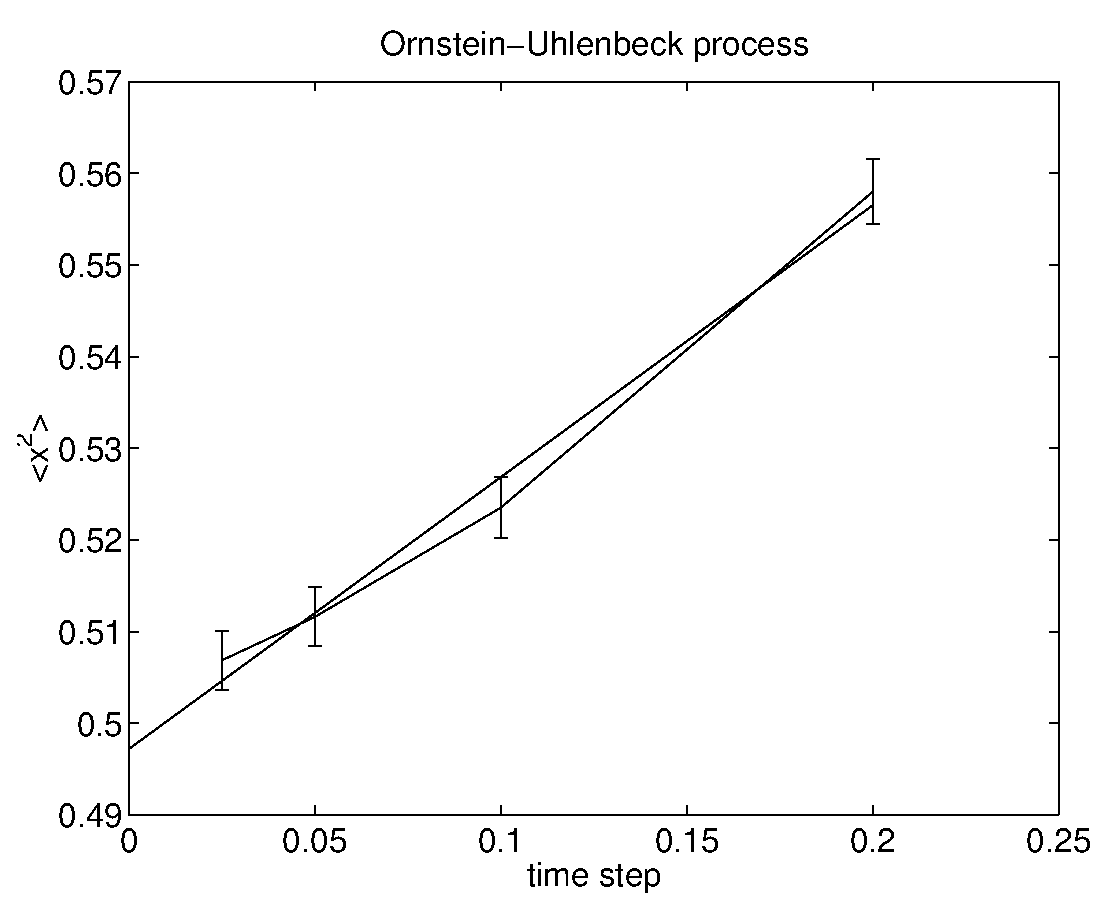
\includegraphics[width=10cm]{./Figures/f_sdeorn_50.eps}
\caption{Results of the simulation of the Ornstein--Uhlenbeck 
process with the stochastic Euler method for different values of 
the time step. The parameters of the Ornstein-Uhlenbeck process
are \texttt{q=1}, \texttt{D=1}. The simulation was run from
\texttt{tstart=0} to \texttt{tend=4} for 50000 realizations.
The timesteps used are \texttt{deltat=0.2, 0.1, 0.05, 0.025}.} 
\end{figure}
The figure clearly shows the expected linear convergence of the 
estimate to the expected exact result. The linear extrapolation 
leads to the estimate $<X^2>|_{t=4}=0.497182$, which is in very 
good agreement with the expected exact result. The simulation took
1729 sec on the laptop.

\subsection{Noise Induced Transitions}
In this second example of the application of the stochastic Euler 
method we want to simulate a stochastic differential equation with
multiplicative noise and consider noise induced transitions.

Let us begin by looking at the following deterministic dynamical 
system
\begin{equation*}
\frac{d}{dt} x(t) = \frac{1}{2} - x(t),
\end{equation*}
for $x \in [0,1]$. Obviously, this dynamical system has one 
fix point at $x_0=1/2$. This fix point can be shown to be 
asymptotically stable. 

We now want to perturb this system by adding a multiplicative 
noise term on the right hand of the above equation of motion.
To be precise we want to replace the deterministic equation of 
motion by the Ito stochastic differential equation
\begin{equation}
\label{SDENOISEIN}
dX(t) = (\frac{1}{2} - X(t))X(t)dt + \epsilon X(t) (1-X(t)) dW(t),
\end{equation}
where $\epsilon <0$

In order to understand the results of the simulation  we want to 
look at the stationary solution of the corresponding 
Fokker--Planck equation. The latter reads
\begin{equation*}
\frac{\partial}{\partial t} = - \frac{\partial}{\partial x} [a(X(t)) P(X,t) ]
      + \frac{1}{2} \frac{\partial^2}{\partial 
      x^2}[b(X(t))P(X,t)],
\end{equation*}
where we have used
\begin{equation*}
a(X(t)) = \left(\frac{1}{2} - X(t)\right) X(t)
\end{equation*}
and
\begin{equation*}
b(X(t)) = [\epsilon X(t) (1-X(t))]^2.
\end{equation*}
Of course, the stationary solution has to satisfy
\begin{equation*}
\lim_{t \rightarrow \infty} \frac{\partial}{\partial t} P(X,t) =0
\end{equation*}
and hence
\begin{equation*}
\frac{d}{dx} [a(X(t)) P(X,t) ] - \frac{1}{2} \frac{\partial^2}{\partial 
      x^2}[b(X(t))P(X,t)] =0.
\end{equation*}
The above equation can be written as
\begin{equation}
\label{DDXJ}
\frac{d}{dx} J(x) =0,
\end{equation}
with 
\begin{equation*}
J(x) = a(X(t)) P(X,t)  - \frac{1}{2} \frac{\partial}{\partial 
      x}[b(X(t))P(X,t)].
\end{equation*}
In order to satisfy Eq. (\ref{DDXJ}) $J$ must be constant. If we 
assume that the stationary density $P_S(x) \longrightarrow 0$ for 
$|x| \longrightarrow \infty$ then the constant in question must be 
zero and we can conclude that
\begin{equation*}
\frac{d}{dx} [b(x) P_S(x)] = 2 a(X)P_S(x).
\end{equation*}
Dividing both sides by $b(x)P_S(x)$ we get
\begin{equation*}
\frac{d [b(x) P_S(x)]}{b(x) P_S(x)} = \frac{2a(x)}{b(x)}.
\end{equation*}
Integrating the above expression gives
\begin{equation*}
\ln [b(x) P_S(x)] = \int_c^x dx' \frac{2a(x')}{b(x')}
\end{equation*}
or
\begin{equation*}
P_S(x) = \frac{N}{b(x)} \exp\{-\phi (x)\},
\end{equation*}
where
\begin{equation*}
\phi(x) = - \int_c^x dx' \frac{2a(x')}{b(x')}.
\end{equation*}
The factor $N$ is a normalization constant to be chosen such that
\begin{equation*}
\int_a^b P_S(x) dx =1.
\end{equation*}

Transposing the above sketched general theory to the stochastic 
differential equation of interest  we get the stationary density,
which is sometimes also called the invariant density,
\begin{equation*}
P_S(x) = \frac{N}{x(1-x)} \exp\left( - \frac{1}
           {\epsilon^2 x(1-x)}\right)
\end{equation*}

Now we are in the position to simulate the stochastic differential
equation (\ref{SDENOISEIN}). This will be done with the help of 
the program \texttt{sdenoisein.m}.

\subsubsection{Listing of the program \texttt{sdenoisein.m}}
\inputlisting{./Listings/sdenoisein.m}
The program generates trajectories of the stochastic process with 
the help of the Euler algorithm. At the end of the simulation we evaluate 
numerically the stationary distribution with the help
of the MATLAB plotting function \texttt{hist}.

In a first run we perform a simulation of 5000 trajectories for 
the following parameters \texttt{xstart=0.5}, \texttt{epsilon=1},
\texttt{tend=4}, and \texttt{deltat=0.01}. The initial condition
was always chosen to be \texttt{xstart=0.5}. The resulting histogram
of the invariant density can be seen in Fig. 
(\ref{F_SDENOISEIN_1}).

\begin{figure}
\label{F_SDENOISEIN_1}
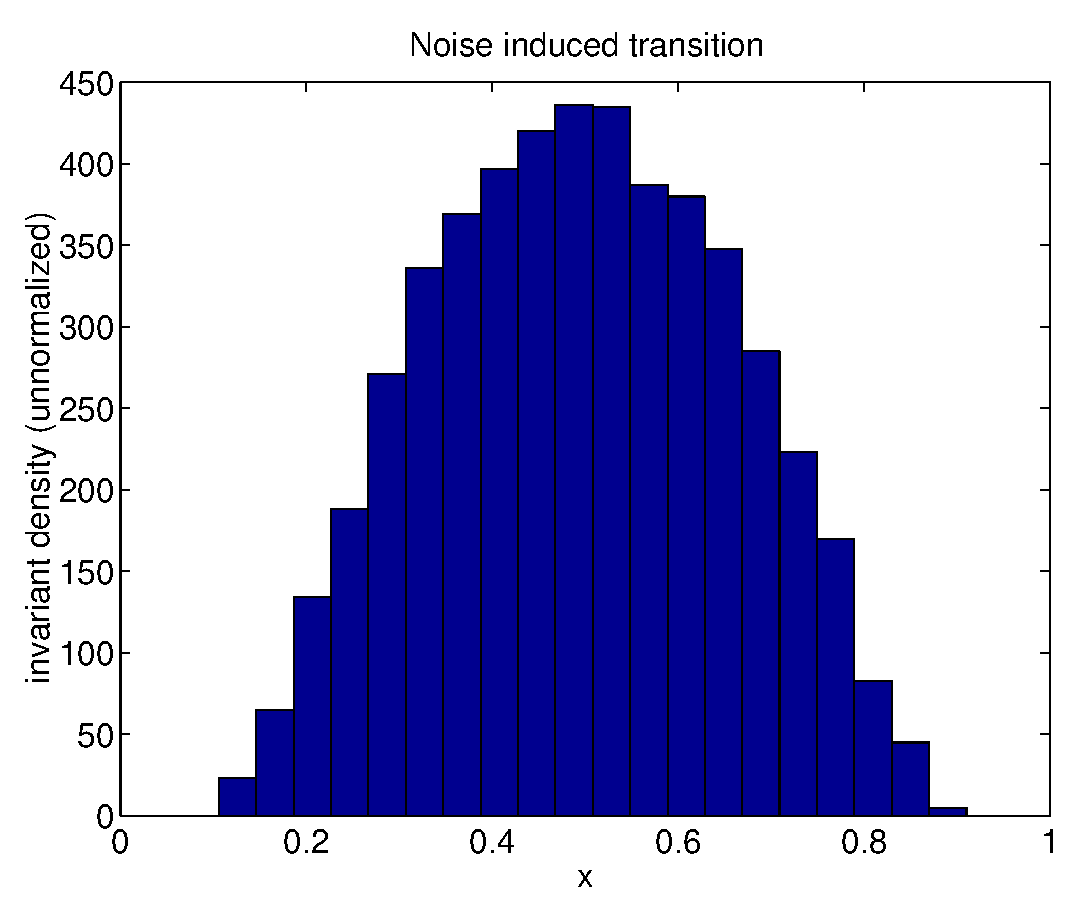
\includegraphics[width=10cm]{./Figures/f_sdenoisein_1.eps}
\caption{Histogram of the invariant density of the stochastic differential 
equation with multiolicative noise. The simulation was run from
\texttt{tstart=0} to \texttt{tend=4} for 5000 realizations.
The initial condition was chosen to be \texttt{xstart=0.5}.
The timestep used was \texttt{deltat=0.01} and the multiplicative noise 
constant was \texttt{epsilon=1}.} 
\end{figure}

It is clear from the histogram that the most probable value of $X$ 
lies around 0.5 and is therefore identical with the fixed point of 
the corresponding deterministic process.

Now we run the program with the same parameters as above but 
choose the multiplicative noise constant to be \texttt{epsilon=3}.
The result of this second simulation can be seen in Fig. 
(\ref{F_SDENOISEIN_2}).
\begin{figure}
\label{F_SDENOISEIN_2}
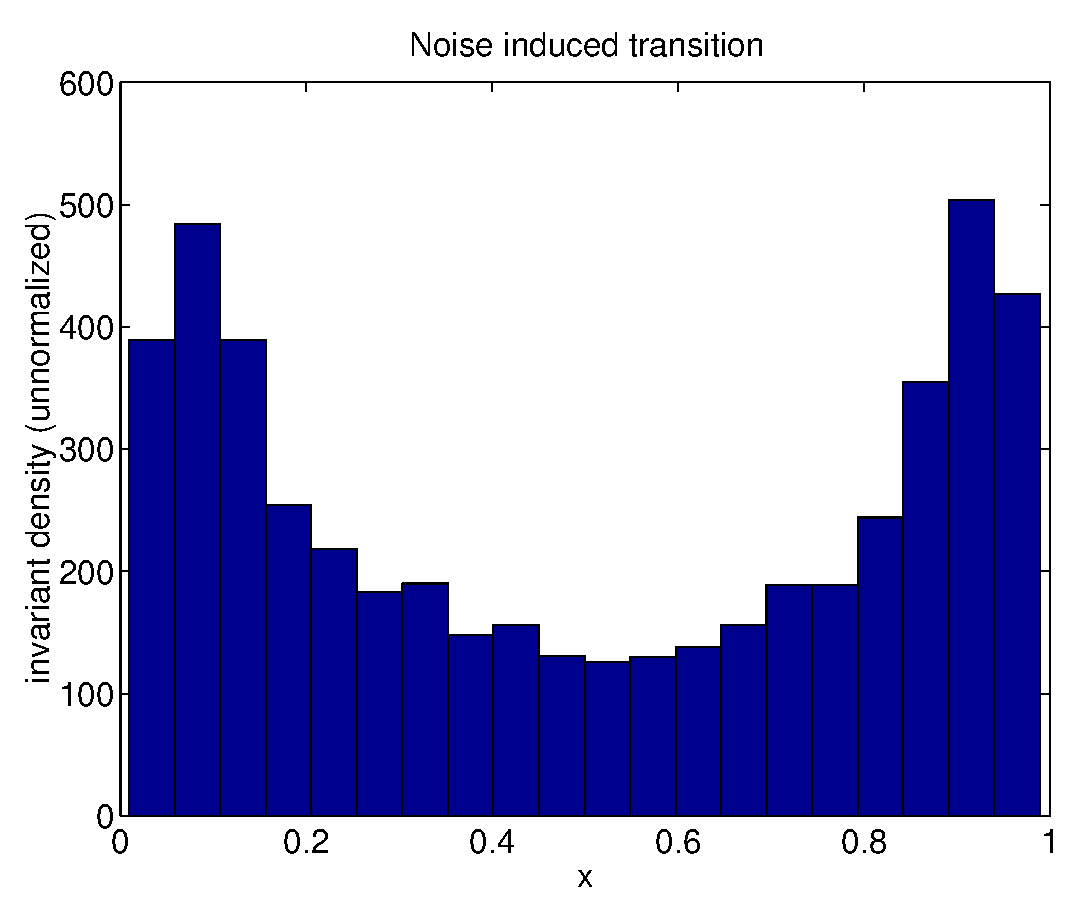
\includegraphics[width=10cm]{./Figures/f_sdenoisein_2.eps}
\caption{Histogram of the invariant density of the stochastic differential 
equation with multiolicative noise. The simulation was run from
\texttt{tstart=0} to \texttt{tend=4} for 5000 realizations.
The initial condition was chosen to be \texttt{xstart=0.5}.
The timestep used was \texttt{deltat=0.01} and the multiplicative noise 
constant was \texttt{epsilon=3}.} 
\end{figure}
It is evident from this figure that the invariant density changes 
its character. Now there is no longer one value of $X$ which is 
more probable. The histogram shows a minimum for $X=0.5$ and two 
equally high maxima at around 0.1 and 0.9. As a consequence of 
the larger noise the system undergoes a "stochastic bifurcation" 
which changes the number of the maxima of the invariant density. 
Such a phenomenon is called a {\em noise induced transition}.

Let us now try to see whether this observation is in agreement 
with the stationary density we have derived at the beginning of 
this subsection. The maxima of the stationary distribution are 
easily evaluated from the equation
\begin{equation*}
0 = \frac{d}{dx}P_S(x_m)
\end{equation*}
which explicitly reads
\begin{equation*}
0= (1-2x_m) [1- \epsilon^2 x_m (1-x_m) ].
\end{equation*}
For $0 < \epsilon <2$ the invariant density has an extremum, 
namley a maximum at $x_m =x_0= 1/2$, which is the fixed point of the 
deterministic equation of motion. For $\epsilon > 2$ the invariant
density posses a minimum at $x_0 =1/2$ and two maxima of equal 
height at $x_{m1,m2}$
\begin{equation*}
x_{m1,m2} = \frac{1}{2} \left(1 \pm  \sqrt{1 - (4/\epsilon^2)} 
\right).
\end{equation*}
Thus for the value of \texttt{epsilon=3} chosen in the second 
simulation the maxima are expected  to be at 0.8727 and 0.1273 
respectively. The histogram reproduced in Fig. (\ref{F_SDENOISEIN_2})
is in agreement with this theoretical prediction.


\section{Stochastic Resonance}
In order to get aquainted with 
the numerical integration of stochastic differential equations we discuss a
phenomenon which occurs as
the response of a nonlinear system in the presence of noise: stochastic 
resonance. For a comprehensive introduction see \cite{Lanzara,Bulsara}. 
We already know that the effect of noise on the time evolution of 
deteministic linear system is rather trivial. If the statistical properties of
the input noise are known it is straightforward to compute the statistical
properties of the output signal. For nonlinear systems the situation changes
dramatically. The presence of the noise influences the evolution of the
system often in a counterintuitive way. The numerical integration of the
corresponding stochastic differential equations allows us to look at the
realizations of the process and to gain insight in these interesting
phenomena. 

The phenomenon of stochastic resonance was proposed by Benzi \textit{et al.}
\cite{Benzi1,Benzi2} in a series of papers in which they address the problem
of the periodic switching of the Earth's climate between periods of relative
warmth and ice ages. It is known from the statistical analysis of continental
ice volume over the last million years that this switching is random and that 
it occurs with an approximate period of 100000 years. It is as well known that
the eccentricity of the Earth orbit varies with roughly the same period. 
However,
the associated variations of the solar energy influx on the earth surface are
so small, that climatologists doubt that  such a small external periodic force
effect might induce such climatic changes. In their seminal papers Benzi
\textit{et al.} represent the global climate with the help of a bistable
``climatic potential''. One minimum of the potential represents a small
temperture typical of an ice age, the other one a more  warm climate.
These authors then show that the weak periodic variation of the eccentricity
together with other random perturbations modelled as additive noise (e.g.
short--term climate fluctuations) might explain the periodicity observed for
the transition between one and the other of the two stable climate 
states. They name this
phenomenon stochastic resonance for the following reason: the
signal--to--noise ratio, i.e. the response of the system, is maximized when a
parameter of the stochastic force is tuned to an optimal value.

It is the aim of this section to introduce the basic principles of stochastic
resonance \cite{McNamara,Gammaitoni} and to simulate a simple model 
showing this phenomenon.
It is clear from the example discussed above that the basic mechanism  of 
stochastic resonance relies upon three essential ingredients:
a bistable system, a periodic driving signal, and a noise signal.

The simplest version of a one--dimensional nonlinear dynamical system 
is the damped anharmonic oscillator with the following equation of motion
\begin{equation}
m \frac{d^2x}{dt^2} + \gamma \frac{dx}{dt} = - \frac{dU(x)}{dx} 
 + \sqrt{D} \chi(t).
\end{equation}
The above Langevin equation describes the motion of a classical particle of
mass $m$ in a potential $U(x)$ and with an additive stochastic force
$\chi(t)$,
where $\chi(t)$
is a Gaussian white noise characterized by
\begin{equation}
\langle \chi(t) \rangle =0; \;\;\; \langle \chi(t) \chi(t')\rangle =
\delta(t - t').
\end{equation}
The potential $U$ is bistable and we assume that it has the simple form
(see figure \ref{fig:BistablePotential})
\begin{equation}
U(x) = -a \frac{x^2}{2} + b \frac{x^4}{4}.
\end{equation}
\begin{figure}[htbp]
  \begin{center}
    \includegraphics[width=\textwidth]{Figures/BistablePotential.eps}
    \caption{The potential $U(x)=-a \frac{x^2}{2} + b \frac{x^4}{4}$ 
      for $a=1$ and $b=1$.}
    \label{fig:BistablePotential}
  \end{center}
\end{figure}
For $a> 0$ the potential $U$ is bistable with an unstable state at $x=0$
and two stable states at $x_s = \pm \sqrt{a/b}$. The stable states are
separated by a barrier of height $\Delta U = a^2/4b$. The system remains
dynamically stable for $b>0$, and becomes monostable for $a \le 0$.
Furthermore we assume that the system is overdamped by neglecting the inertial
term $m d^2x/dt^2$. 
Rescaling the resulting Langevin equation with the damping constant
$\gamma$  we finally obtain the so--called stochastic Ginzburg--Landau
equation
\begin{equation}
\label{Stoch_Ginzburg_Landau}
\frac{dx(t)}{dt} = ax - bx^3 + \sqrt{D} \chi(t),
\end{equation}
an equation which is often encountered in the theory of nonequilibrium
critical phenomena. 

\subsection{Reaction Rate Theory}
Let us now investigate some fundamental properties of the above dynamical
system. We begin by considering the case $D=0$ (no fluctuations). If the 
system is initially in a stable state it remains there for ever. 
The typical local
time scale is the relaxation time $\tau_r$ inside the wells. This time scale 
can be determined by considering small variations around the 
minimum of the well.
To do so we linearize Eq. (\ref{Stoch_Ginzburg_Landau}) 
around the stable state $x_s = \sqrt{a/b}$ with the help of
\begin{equation}
x(t) = x_s + \delta x(t)
\end{equation}
and obtain
\begin{equation}
\frac{d(\delta x)}{dt} = -2a \delta x.
\end{equation}
Thus, the  time scale $\tau_r$ of the relaxation inside the wells is
\begin{equation}
  \tau_r = \frac{1}{2a} = \frac{1}{U''(x_s)}.
\end{equation}

The situation changes in the presence of noise. The fluctuating forces allow
the system to jump between the two stable states. If the noise strength $D$ 
is small compared to the barrier height, these jumps are rare events. 
It is a well--know result of Kramers reaction--rate theory (see e.g.
\cite{Haenggi:Kramers}) that the mean escape time $T_e(x)$ out of one basin of
attraction can be written for sufficiently low noise ($\Delta U/D \gg 1$)in 
the form of the Arrhenius law
\begin{equation}
  \label{eq:Arrhenius}
  T_e(x) = A \exp(\Delta U(x)/D),
\end{equation}
where $A$ is a prefactor which depends on the form of the potential. For the
special potential we consider here, performing a Gaussian approximation of the
potentail around the minimum and the maximum and using the condition
$\Delta U/ D >> 1$ one gets the so--called Kramers
formula (or Arrhenius formula) for the escape time of a bistable system
\begin{equation}
\label{eq:Kramers}
  \tau_k = \frac{2\pi}{\sqrt{|U''(0)|U''(x_s)}} \exp [ 2 \Delta U / D ].
\end{equation}
The escape time $\tau_k$ is the global time scale of the bistable system.
The physical content of the assumptions we stated above is the following
one: The Kramers time $\tau_k$ is derived under the assumption that the
probability density within a well is roughly in equilibrium when the escape
takes place. Thus, the condition $\Delta U/D \gg 1$ guarantees that the two
time scales, the relaxation time and the Kramers time are different. The
system relaxes quickly (on a short time scale) to a local equilibrium at the
stable states and approaches global equilibrium (transitions over the barrier)
on a slow time scale. It follows from Eq. (\ref{eq:Kramers}) that
\begin{equation}
  \frac{\tau_k}{\tau_r} = 2 \sqrt{2} \pi \exp(2 \Delta U /D) \gg 1.
\end{equation}
The rate to jump over the barrier $W_k$ is obviously the inverse escape time
\begin{equation}
  w_k = \tau_k^{-1} = \frac{a}{\sqrt{2} \pi} \exp(-2 \Delta U/D).
\end{equation}

\subsection{The Stochastic Resonance}
Having reviewed some basic results of the theory of nonlinear stochastic
systems we are now ready to look at the phenomenon of stochastic resonance.
In the preceeding subsections we made use only of two of the basic ingredients
of the recipe for stochastic resonance. The phenomenon only occurs in the
presence of a periodic driving signal. If we add such a signal to the bistable
system just considered its dynamics will be governed by the following Langevin
equation
\begin{equation}
  \frac{dx}{dt} = - \frac{\partial U(x,t)}{\partial x} + \sqrt{D} \chi(t), 
\end{equation}
where the bistable potential takes now the form
\begin{equation}
\label{eq:bistablepotential}
  U(x,t) = -a \frac{x^2}{2} +b \frac{x^4}{4} - Ax \cos(\omega_s t),
\end{equation}
where $A$ and $\omega_s= 2 \pi/T_s$ are the amplitude 
and the frequency of the periodic
signal. As a consequence of the periodic forcing term the potential tilts
periodically between up  and down. When the periodic force is at its
maximum (or minimum)  the difference between the escape rates from the two
states is maximum. The periodic forcing is assumed to be so
weak that it can not let the particle roll periodically from one potential
well into the other one. Nevertheless, the noise--induced hopping beween the
two wells  may become synchronized with the weak periodic forcing. This is 
signature of stochastic resonance. Stochastic resonance manifests itself by a
synchronization of activated hopping between the potential minima with the
weak periodic forcing. 

The manifestation of the phenomenon may be visualized with the help of the
output signal. It is clear that in the absence of the periodic driving
the escape process is induced by the fluctuating force and is random. Thus, in
this case the output signal $x(t)$ looks like dichotomous noise. The
probability density of residence times between two jumps is exponential
\begin{equation}
  P(t) = \frac{1}{\tau_k} \exp(-t/\tau_k),
\end{equation}
where the Kramers time can be
interpreted as the mean residence time spent by the system in one well.
The periodic driving force alters this situation. The modulation synchronizes
the hopping. The output signal reveals a quasiperiodic contribution to the
jump process, which has a maximum if the system jumps, on average, two times
per cycle of the external forcing. This is the stochastic resonance condition,
which for small driving frequencies $\omega_s \ll \omega_k$ 
can be approximated by \cite{Jung}
\begin{equation}
\label{eq:ResonanceCondition}
  T_s = 2 \tau_k = \frac{2 \pi \sqrt{2}}{a} \exp(2 \Delta U / D).
\end{equation}
The same condition formulated in terms of the noise intensity reads
\begin{equation}
\label{eq:ResonanceConditionD}
  D_0 = \frac{2 \Delta U}{\ln(a/(\sqrt{2} \omega_s))}.
\end{equation}
At this resonance condition the coherent contribution of the jump process has
a maximum.

Now that we have learned the basic aspects of stochastic resonance let us 
write a program to simulate it. Before doing so it is very helpful to write
the basic equations of motion in dimensionless form. To this end we write
the bistable potential (\ref{eq:bistablepotential}) in the form
\begin{equation}
  \label{eq:bistabledimless}
  U(x,t) = \Delta U \left[ -2\left( \frac{x}{x_s} \right)^2 
                           + \left( \frac{x}{x_s} \right)^4 \right] - 
                 U_1 \left(\frac{x}{x_s} \right) \cos(\omega_s t),.
\end{equation}
where $U_1 = A x_s$. The Langevin equation of motion can then be written as
\begin{equation}
  \label{eq:langevindimless1}
  \frac{dx}{dt} = 4 \Delta U \left( \frac{x}{x_s^2} - 
                   \frac{x^3}{x_s^4} \right)
                  + \frac{U_1}{x_s} \cos(\omega_s t)
                  + \sqrt{D} \xi(t).
\end{equation}
If we devide the above equation through $4 \Delta U$ and multiply it by $x_s$
\begin{equation}
  \label{eq:langevindimless2}
  \frac{1}{x_s} \frac{x_s^2}{4 \Delta U} \frac{dx}{dt} 
 =  \left( \frac{x}{x_s} - 
                   \frac{x^3}{x_s^3} \right)
                  + \frac{U_1}{ 4 \Delta U } \cos(\omega_s t)
                  + \frac{x_s}{4 \Delta U}\sqrt{D} \xi(t).
\end{equation}
If we now choose the unit of length to be $x_s$ and the time unit to be
$1/a$, note that $x_s^2/4 \Delta U = 1/a$, the dimensionless form of the above
equation reads
\begin{equation}
  \label{eq:langevindimless3}
  dx 
 =  \left( x - 
              x^3 \right)dt 
                  + \frac{U_1}{ 4 \Delta U} \cos(\omega_s t)dt
                  + \sqrt{D} \eta(t) \sqrt{dt},
\end{equation}
where for notational convenience we have named $x$ and $t$ to denote the 
corresponding dimensionless quantities and $D$ denotes the dimensionless
noise intensity. Recall, that in the units defined above $D$ has the dimension
$a x_s^2$.

%%%% ????????????? \inputlisting{StochasticResonance.java}

Before running the program let us formulate the resonace condition in
dimensionless units. It follows from Eq. (\ref{eq:ResonanceConditionD}) that
\begin{equation}
  \label{eq:ResonanceConditionDless}
  D_0= \frac{1}{2 \ln (1/\sqrt{2} \omega_s)}.
\end{equation}
To give a numerical example, for $\omega_s= 0.1$ the  time scale matching
condition states that we have to choose $D= 0.2556$. Let us run now the
program keeping first $\omega_s$ fixed and varying $D$ and then keeping $D$
fixed and varying $\omega_s$.



Here comes the simulation and the discussion.


Now we could discuss:
\begin{itemize}
\item the periodic response
\item the signal to noise ratio
\end{itemize}

Let us finally look at the spectrum of the output signal. ...



Since its original formulation the phenomenon of stochastic resonance has been
observed in several physical and biological systems. These observations are
reviewed in 
\cite{Gammaitoni} and the introductory article \cite{Bulsara} .


%%%%%%%%%%%%%%%%%%%%%%%%%%%%%%%%%%%%%%%%%%%%%%%%%%%%%%%%%%%%%%%%%%

\section{Exercises}

\begin{Ex}
\label{Johnson_Noise}
\textbf{Johnson Noise \cite[]{gillespie:96} } \\
Johnson noise is the thermally generated electrical noise appearing in a conductor. 
Assume we have a rigid wire loop of self-inductance $L$ and resistance $R$ at
absolute temperature $T$. We can visualize this using the figure below. 
\begin{center}
\includegraphics[width=5cm]{f_johnson.eps}
\end{center}
There is no external potential, just the interactions between the conducting
electrons and the vibrations of the atomic lattice give rise to a temporally \text{var}ying
electromotive force in the loop (for details see \cite[]{gillespie:96}). 

The circuit equation gives (the integral of the electric potential around the 
loop must be zero)
$$ -RI(t)+V(t)-L\frac{dI(t)}{dt}=0.$$
Taking averages gives (assume $<V(t)>=0$) $$ -L\frac{d<I(t)>}{dt} =R<I(t)> .$$
If we can measure $I(t)$ we have an experimental way of determining $R$ and $L$.

We rewrite the first equation using $\tau:=L/R$ and $V(t):=Lc^{1/2}\Gamma(t)$, where
$\Gamma(t)$ is a Gaussian white noise and $c>0$ constant:
$$ \frac{dI(t)}{dt}=-\frac{1}{\tau}I(t)+c^{1/2}\Gamma(t) .$$
This is just the Langevin-equation for an Ornstein-Uhlenbeck process with
relaxation time $\tau$ and diffusion constant $c.$
The diffusion constant $c$ can be calculated by using the equipartition
theorem of statistical mechanics and applying the results for the 
Ornstein-Uhlenbeck process. We get $c=2kTR/L^2.$

Write a program to solve the Langevin equation for $I(t)$ with the initial
condition $I(t)=i_0.$ Use the Euler method for solving stochastic
differential equations. Use the three different sets of parameters:
\begin{itemize}
\item $\tau=1, c=1, i_0=0, \Delta t=0,001 $
\item $\tau=1, c=1, i_0=0, \Delta t=0,0001 $
\item $\tau=0,001, c=1.000.000, i_0=0, \Delta t=0,001 $
\end{itemize}
(Remark: the first and the third parameter set lead to the same
constant $\tau c^{1/2}$ for discussing $\tau\to 0$, the limit to Gaussian
white noise.)

The exact solution is ($\mathbf{N}( , )$ denotes a normal distribution):
$$ I(t)= \mathbf{N}\left(i_0e^{- \frac{R}{L}(t-t_0)} , \frac{kT}{L}
        \left(1-e^{-2\frac{R}{L}(t-t_0)}\right) \right) .$$

Also calculate the (auto-)covariance function $ C_I(t'):=\text{cov}(I_s(t),I_s(t+t')) $
(the subscript $s$ indicates that the process should be stationary)
and analyze the spectrum thereof - use a log-log plot for the
spectrum. The spectrum is the cosine transform of $C_I$.
\end{Ex}


%%%%%%%%%%%%%%%%%%%%%%%%%%%%%%%%%%%%%%%%%%%%%%%%%%%%%%%%%%%%%%%%%%%%%

\bibliographystyle{peter}
\bibliography{V_98,simulit}



%%% Local Variables: 
%%% mode: latex
%%% TeX-master: t
%%% End: 


%%% Chapter 6 
\include{Chap6}

%%% Chapter 7 
\chapter{Molecular Dynamics}

\section{Introduction}
\subsection{Statistical Properties of Fluids}
With this chapter we begin the description of the application
of stochastic methods to the simulation of physical systems. Computer
simulations are an essential tool for the understanding of complex physical
systems which complement the more traditional theoretical and experimental
approaches. Computer simulations offer the possibility to investigate  the
structural, dynamical and thermodynamical properties of interesting systems. 
Within statistical physics essentially two different simulation approaches
have been developed: Molecular Dynamics (MD) methods, which we will consider
in this chapter  and Monte Carlo methods
(MC), which will be introduced in the next one.

The basic idea of the Molecular Dynamics approach is the following one: We
know that fluids, e.g. gases and liquids, are systems which are composed of a
large number of particles which are mutually interacting. 
Although the most
fundamental description of matter at the microscopic level is, of course,
quantum mechanical, in the framework of Molecular Dynamics it is assumed that
we can describe the motion of a single atom or molecule  by the classical
laws of motion, i.e., by Hamilton equations of motion. This assumption is
justified, if the mean de Broglie wavelength of an atom is much smaller
then the mean distance between atoms. This condition is satisfied if the
density of the fluid is sufficiently low  or if the temperature of the fluid
is sufficiently high. Thus, it is the aim of Molecular Dynamics to
understand the macroscopic thermodynamic and dynamical properties of a fluid
starting from the microscopic equations of motions of its atoms. To put it
differently: Molecular Dynamics is the direct simulation of the
equations of motion of a system composed of $N$ classical mutually 
interacting particles. The main numerical problem we have to address in this
chapter is the development of an algorithm for the numerical integration of
the equations of motion of $N$ particles.

The numerical solution of classical equations of motion looks like a
deterministic process. Why is it then relevant for us? 
The answer is very easy. Molecular Dynamics is a beautiful
example of a deterministic Markov process. The temporal evolution of the system
is of course deterministic, but the initial condition, the initial
configuration of the atoms in the fluid is random! 
The initial position as well as the initial velocities of the particles are
random. A Molecular Dynamics
simulation solves the Liouville equation, which as we know 
is the typical example of the differential Chapman--Kolmogorov equation 
of a deterministic Markov process.

\subsection{Some Historical Comments}
The Molecular Dynamics method has been proposed by Alder and Wainwright
in 1957 \cite{AlderWainwright57,AlderWainwright59}. They investigated a fluid
composed of hard spheres. In this pioneering simulation the particles moved
with constant velocity between two elastic collisions. The first simulation of
a real fluid was published in 1964 by Rahman \cite{Rahman}. He simulated
liquid Argon assuming a Lennard-Jones potential for the pair interaction
between the atoms (see below). The equations of motion were integrated using a
stepwise algorithm. It is worth mentioning a citation classic in this context,
namely the paper by Verlet \cite{Verlet67,Verlet68}, in which the 
algorithm for the  integration of the equations of motion, 
which bears his name has been proposed. Since this time Molecular Dynamics
developed to a standard tool in statistical physics. We just want to mention
some important steps. 1968 a diatomic molecular
fluid was simulated for the first time \cite{HarpBerne}. 1971 Rahman and
Shillinger reported the simulation of liquid water. In the same year Woodcock
investigated a fluid with Coulomb interactions -- melted KCl. In 1973 
Barojas, Levesque and Quentrec simulate rigid molecules. In 1977 Camman, Gelin
and Karplus apply Molecular Dynamics to the investigation of proteins. 
The Molecular Dynamics simulation we mentioned were all concerned with
equilibrium properties of fluids. 

At the beginning of the seventies
Non--Equilbrium Molecular Dynamics (NEMD) was developed, which allowed also the
investigation of the behaviour of fluids in typical non-equilibrium situations,
e.g., fluids in thermal gradients, or fluid in shear flow.

At the beginning of the eighties two important papers appeared which reported
on the possibility to include also quantum mechanical effects in the MD
simulations.

\subsection{The Equations of Motion}
The classical Molecular Dynamics algorithm solves the equation of motion for a
set of $N$ particles. A mechanical system with $3N$ degrees of freedom is
fully characterised by a set of $3N$ generalised coordinates $q_i$, 
$i=1, \ldots, 3N$ and of $3N$ generalised momenta $p_i$, 
$i=1, \ldots, 3N$. For a given Hamiltonian $H$ the equations of motion
read
\begin{displaymath}
  \dot{q}_i = \frac{\partial H}{\partial p_i} \;\;\; \mbox{for} 
 \;\;\; i=1, \ldots, N
\end{displaymath}
and
\begin{displaymath}
  \dot{p}_i = - \frac{\partial H}{\partial q_i} 
      \;\;\; \mbox{for} \;\;\; i=1, \ldots, N.
\end{displaymath}
In many cases the potential is conservative and Cartesian coordinates
$x_i$ and the velocities $v_i = p_i/m_i$ are used, where $m_i$ denotes the
mass of particle $i$. In these cases the Hamiltonian may be written as
\begin{displaymath}
  H(\{p_i,x_i\}) = \sum_{i=1}^N \frac{p_i^2}{2m_i} + V(\{x_i\}).
\end{displaymath}
For this special case the equations of motion read
\begin{equation}
   \label{HamiltonEqs}
  \dot{x}_i = v_i \;\;\; \mbox{and} \;\;\; m_i \dot{v}_i = F_i,
\end{equation}
where the forces are
\begin{displaymath}
  F_i = - \frac{\partial}{\partial x_i} V(\{x_i\}).
\end{displaymath}
It is clear from Eq. (\ref{HamiltonEqs}) that the calculation of the
velocities $v_i$ is not essential, since the Hamiltonian equations of motion 
(\ref{HamiltonEqs}) are  equivalent to the Newtonian ones
\begin{displaymath}
  m_i \frac{\partial^2}{\partial t^2}{x}_i = F_i(\{x_i\}).
\end{displaymath}
Having recalled the equations of motion of classical system composed of $N$
particles we have to address the two following questions which are essential
to all Molecular Dynamics simulations: How do we calculate the forces? How do
we integrate the equations of motion? These questions will be addressed in the
following two sections.


\section{Simple Models and Interaction Potentials}
In the first Molecular Dynamics simulation the classical fluid of interest was
liquid Argon. In liquid argon the atoms are chemically inert and can be
assumed to be spherical. For this reason the forces between any two atoms 
depend only on the distance between the atoms. Thus, considering a system of
$N$ atoms the potential energy may be written as
\begin{displaymath}
  V =  \underbrace{\sum_i V_1(\vec{r}_i)}_{\textrm{external field}} + 
       \underbrace{\sum_{i}\sum_{j>i} V_2(\vec{r}_i,\vec{r}_j)}_{
            \textrm{Pair interaction}} +
       \underbrace{\sum_{i} \sum_{j>i} \sum_{k>j>i} V_3(\vec{r}_i,\vec{r}_j,
        \vec{r}_k)}_{\textrm{3-particle interaction}}
       + \cdots,
\end{displaymath}
where the first sum on the right--hand side represents the potential of an
external field, the second sum represents the pair interactions, the 
third sum represents the three particle interaction, and so on. Of course, the
calculation of the three particle interaction and of interaction of higher
order are very expensive from a computational point of view. Fortunately, in
praxis these contributions to the potential can be neglected. For simple
fluids, like Argon, the pairwise
interaction $V_2$ depends only on the magnitude of the separation 
$|\vec{r}_i - \vec{r}_j|$ between the atoms $i$ and $j$. For the moment we
will also assume that there is no external field acting on the particles, so
that we are left only with the pair interaction potential $V_2$.

This potential can, of course, be determined from first principles using
quantum mechanics. These calculations turn out to be very difficult and so one
relies upon phenomenological forms for the potential $V_2$. For argon and other
noble atoms with closed electronic shells, the mutual polarisation of each
atom induces an attractive interaction, which is known as the van der Waals
interaction. This interaction has the form
\begin{displaymath}
  V_{vdW} \approx -I \left( \frac{\sigma}{r}\right)^6,
\end{displaymath}
where $I$ is the ionisation potential of the atom, and $\sigma$ is a
length scale characterising the size of the atom. 

When two argon atoms approach each other so closely that their electron
shells overlap, the Pauli exclusion principle causes an effective repulsive
force. This force increases rapidly with decreasing separation between
the atoms. This effect is called \textit{core repulsion}. The most common
phenomenological form
of the potential $V_2$ is the Lennard--Jones potential
\begin{displaymath}
  V_{LJ} = 4 \epsilon \left[\left( \frac{\sigma}{r}\right)^{12}
                           - \left( \frac{\sigma}{r}\right)^6 \right]. 
\end{displaymath}
A plot of the Lennard--Jones potential can be seen in Fig. 
(\ref{Fig:LennardJones}).
It is important to notice that $V_{LJ}=0$ at $r= \sigma$ and that 
$V_{LJ}(r)$ is essentially equal zero for $r>3\sigma$. The parameter 
$\epsilon$ is the depth of the potential at the minimum. The minimum occurs at
the separation $r= 2^{1/6}\sigma$. The parameters
$\epsilon= 1.65 \times 10^{-21} J$ and $\sigma = 3.4 A$ are in good agreement
with the experimental properties of liquid argon.
 
\begin{figure}
\label{Fig:LennardJones}
\caption{Plot of the Lennard--Jones potential $V_{LJ}$. The potential is
  characterised by the length scale $\sigma$ and by the energy $\epsilon$.}
\end{figure}

In order to study some special properties of fluids it is sometimes useful to
consider less general potentials. The hard--sphere potential is defined as
\begin{displaymath}
  V_{hs}(r) = \left\{ 
                \begin{array}{ll}
                 \infty, &\hspace{1cm} (r<\sigma) \\
                 0, & \hspace{1cm} (\sigma \le r).
                \end{array}
             \right.
\end{displaymath}
The hard sphere potential is depicted in Fig. (\ref{Fig:HardSphere}).

\begin{figure}
\caption{Plot od the hard shere potential.}
\label{Fig:HardSphere}
\end{figure}

The Lennard--Jones potential may be approximated by the square well potential
\begin{displaymath}
  V_{sw}(r) = \left\{
              \begin{array}{ll}
                   \infty, & \hspace{1cm} (r < \sigma_1) \\
                    - \epsilon, & \hspace{1cm} (\sigma_1 \le r < \sigma_2) \\
                    0, & \hspace{1cm} (\sigma_2 \le r)  
               \end{array}
              \right. 
\end{displaymath}
The square well potential is depicted in Fig. (\ref{Fig:SquareWell}).

\begin{figure}
\label{Fig:SquareWell}
\caption{Plot of the square well potential}
\end{figure}

The soft sphere potential is defined as
\begin{displaymath}
  V_{ss}(r)= \epsilon \left( \frac{\sigma}{r} \right)^{\nu},
\end{displaymath}
where $\nu$ is a parameter controlling the strength of the potential. For
increasing $\nu$ the potential gets "harder". In Fig. (\ref{Fig:SoftSphere})
we plot the soft sphere potential for two values of $\nu$.

\begin{figure}
\label{Fig:SoftSphere}
\caption{Plot of the soft sphere potential for $\nu=1$ and $\nu=12$.}
\end{figure}

We mentioned in the introduction to this chapter that Molecular Dynamics
simulations may also be used to investigate fluids with Coulomb interaction.
In this case the potential reads
\begin{displaymath}
  V_{zz} (r_{ij}) = \frac{z_i z_j}{4 \pi \epsilon_0 r_{ij}},
\end{displaymath}
where $z_i$ and $z_j$ denote the charge of the ion $i$ and $j$, respectively.


\section{Algorithms for the Integration of Newton's Equations of Motion}
In this section we want to get acquainted with algorithms for the numerical
integration of Newton's equations of motion. We will write them for notational
convenience as
\begin{displaymath}
  \frac{d^2}{dt^2} x(t) = f(x),
\end{displaymath}
where $x(t)$ and $f$ are vectors with $3N$ coordinates. 
Probably, you will already have heard a course on numerical methods for
physics and will therefore suppose that the right algorithms are Runge--Kutta
algorithms. As you may remember Runge--Kutta algorithms require the 
evaluation of the force several times per time step. Unfortunately,
in Molecular Dynamics simulations the evaluation of the forces is the most
time consuming step during the simulation. So, Runge--Kutta methods are not a
good choice. We will therefore have to look at algorithms which require at
most one or two evaluations of the forces per time step.

In the following we will consider finite difference methods in order to compute
the values of $x_{n+1}$ and $v_{n+1}$ at time $t_{n+1} = t_n + h$,
where $h$ denotes the time step of the integration. $\Delta t$ must be
chosen in such a way that the integration methods generates a stable
solution. For a conservative system $h$ must be chosen small enough to
ensure that the total energy is conserved within the required accuracy.

\subsection{Euler Methods}
The easiest but not particularly precise choice are Euler algorithms. 
We write Newton's equation of motion in the following form
\begin{displaymath}
  \frac{d}{dt} x = v(t)
\end{displaymath}
and
\begin{displaymath}
  \frac{d}{dt} v = f(t).
\end{displaymath}
In order to derive an integration algorithm we look at 
$x_{n+1} = x(t_n +h)$ and $v_{n+1} = v(t_n +h)$ and expand in a
Taylor series around $x(t_n)$ and $v(t_n)$, respectively. Keeping terms up to
second order in $h$ we obtain the Euler method
\begin{eqnarray*}
  x_{n+1} &=&  x_n + h v_n + \frac{1}{2} h^2 f_n  \\
  v_{n+1} & = & v_n + h f_n.
\end{eqnarray*}
The Euler algorithm can be improved by expanding it to a predictor--corrector
scheme. The predictor step of the modified Euler algorithm reads
\begin{eqnarray*}
  y_{n+1} &=& x_n + h v_n + \frac{1}{2} h^2 f_n  \\
   f^{\ast} & = & \frac{1}{2} \left( f_n + f(y_{n+1}) \right)
\end{eqnarray*}
and the corresponding corrector step is
\begin{eqnarray*}
  x_{n+1} & = & x_n + h v_n + \frac{1}{2} h f_n \\
          & = & y_{n+1} + \frac{1}{4} 
           \left( f(y_{n+1}) - f_n \right) \\
    v_{n+1} & = & v_n + h f^{\ast},
\end{eqnarray*}
where $f_{n+1} = f(x_{n+1})$.
This modified Euler algorithm is more accurate then the original version, but
it implies a double evaluation of the forces. By choosing
\begin{displaymath}
  f_{n+1} = f(y_n)
\end{displaymath}
only one evaluation of the forces is necessary. This last predictor/corrector
Euler algorithm turns out to be less accurate then the modified Euler
algorithm.

\subsection{The Gear Algorithm}
Some Molecular Dynamics simulations employ the Gear algorithm. The Gear
algorithm is a systematic predictor--corrector scheme. In the first predictor
step the positions and the velocities are developed in a Taylor series. Then
the accelerations, which in general are different from those predicted by the
Taylor expansion,  are calculated from the new positions. From the difference
of the two accelerations one calculates in the second corrector step corrections
to the positions and the velocities. Depending on the order of the Taylor
expansion which are considered one obtains Gear algorithms of different order.

Here, we just want to present the algorithm and refer the interested reader to
the original literature \cite{Gear}. The algorithm is based on the definition
of the vector
\begin{displaymath}
  \vec{x}_n = (x_n, h x_n', \frac{1}{2} h^2 x_n'', \frac{1}{3!} h^3 x_n'''
           , \ldots).
\end{displaymath}
With the help of this vector the predictor step is formulated as
\begin{displaymath}
  \vec{y}_{n+1} = A \vec{x}_n,
\end{displaymath}
and the corrector step reads
\begin{displaymath}
  \vec{x}_{n+1} = \vec{y}_{n+1} + \vec{a} \frac{1}{2} h^2
               \left( f(y_{n+1}) - y_{n+1}''\right).
\end{displaymath}
The coefficients of the matrix $A$ and of the vector $\vec{a}$ in the
predictor and in the corrector step have to be chosen differently for every
different order. To give an example, in the Gear algorithm of 4th order
the matrix $A$ is
\begin{displaymath}
  A = \left( \begin{array}{cccc}
                    1 & 1 & 1 & 1 \\
                    0 & 1 & 2 & 3 \\
                    0 & 0 & 1 & 3 \\
                    0 & 0 & 0 & 3
              \end{array} 
          \right)
\end{displaymath}
and the vector $\vec{a}$ is given by
\begin{displaymath}
  \vec{a} = \left( 
             \begin{array}{c}
               1/6 \\
               5/6 \\
               1 \\
               1/3
              \end{array}
             \right).
\end{displaymath}
For the Gear algorithm of 5th order $A$ and $\vec{a}$ have to be chosen as
\begin{displaymath}
A =   \left( 
             \begin{array}{ccccc}
                    1 & 1 & 1 & 1 & 1\\
                    0 & 1 & 2 & 3 & 4\\
                    0 & 0 & 1 & 3 & 6\\
                    0 & 0 & 0 & 3 & 4 \\
                    0 & 0 & 0 & 0 & 1
              \end{array}
             \right)
\end{displaymath}
and
\begin{displaymath}
  \vec{a} = \left( 
                 \begin{array}{c}
                   19/20 \\
                    3/4 \\
                    1 \\
                    1/2 \\
                    1/12
                  \end{array}
                    \right).
\end{displaymath}

\subsection{Verlet and Beeman Algorithm}
\subsubsection{The Verlet Algorithm}
One of the most popular algorithms for the integration of Newton's equations
of motion is the Verlet algorithm. The Verlet algorithm is less accurate then
the Gear algorithm but it is simpler and requires much less memory. 
Let us consider the Taylor expansion of $x(t_n + h)$ and of $x(t_n - h)$
\begin{eqnarray*}
  x_{n+1} & = &  x_n + h x_n' + \frac{1}{2} h^2 x_n'' 
         + \frac{1}{3!} h^3 x_n''' + \cdots \\
x_{n-1} & = &  x_n - h x_n' + \frac{1}{2} h^2 x_n'' 
         - \frac{1}{3!} h^3 x_n''' + \cdots 
\end{eqnarray*}
Adding the two above expansions we get
\begin{displaymath}
  x_{n+1} = 2 x_n - x_{n-1} + h^2 f(x_n).
\end{displaymath}
This is the Verlet algorithm. Note that velocities do not appear in the above
equation. If knowledge about the velocities is needed, i.e., for computing
the kinetic energy, they can be computed as central differences
\begin{equation}
\label{Eq:VerletV}
  v_n = (x_{n+1} - x_{n-1})/2h.
\end{equation}
Note, that the Verlet algorithm is not self--starting, since it requires the
knowledge of $x_n$ and $x_{n-1}$. If initially only $x_n$ and $v_n$ are known,
$x_{n+1}$ can be computed in the first step as
\begin{displaymath}
  x_{n+1} = x_n + h v_n + \frac{1}{2} h^2 f(x_n).
\end{displaymath}
The global errors associated with the Verlet algorithm are third order for the
positions and second--order for the velocities.

\subsubsection{The Velocity Form of the Verlet Algorithm}
A mathematically equivalent version of the Verlet algorithm is the so called
velocity Verlet algorithm, which is given by
\begin{displaymath}
  x_{n+1} = x_n + v_n h + \frac{1}{2} f_n h^2
\end{displaymath}
and
\begin{displaymath}
  v_{n+1} = v_n + \frac{1}{2}(f_{n+1} + f_n) h.
\end{displaymath}
The velocity Verlet algorithm is self--starting and minimises the errors. The
equivalence of the two algorithms is best seen in the following way.
Adding the expressions for $x_{n+1}$ and for $x_{n-1}$ and eliminating the
velocities with the help of the corresponding expression we obtain immediately
the Verlet algorithm from the velocity Verlet algorithm. In the following we
will refer the velocity Verlet algorithm as \textit{the} Verlet algorihm. 

\subsubsection{The Beeman Algorithm}
Another well--known algorithm is the Beeman algorithm, which also avoids the
round--off errors of the original Verlet algorithm. It can be written in the
following form
\begin{equation}
\label{Eq:BeemanX}
  x_{n+1} = x_n + v_n h + \frac{1}{6} (4 f_n - f_{n-1}) h^2
\end{equation}
and
\begin{equation}
\label{Eq:BeemanV}
  v_{n+1} = v_n + \frac{1}{6} (2 a_{n+1} + 5 f_n - f_{n-1})h.
\end{equation}
The equivalence of the Beeman algorithm with the Verlet algorithm can be
demonstrated in the following way. It follows from (\ref{Eq:BeemanV})
that
\begin{equation}
  \label{eq:BeemanV1}
  h v_{n-1} = x_n - x_{n-1} - \frac{1}{6} h^2(4 f_{n-1} - f_{n-2}).
\end{equation}
Inserting (\ref{eq:BeemanV1}) into Eq. (\ref{Eq:BeemanV}) for $v_n$ we obtain
\begin{equation}
  \label{eq:BeemanV2}
  v_n = x_n - x_{n-1} + \frac{1}{3} h^2 f_n + \frac{1}{6} h^2 f_{n-1}.
\end{equation}
Finally, the original Verlet algorithm is recovered by inserting the above
equation (\ref{eq:BeemanV2}) into Eq. (\ref{Eq:BeemanX}).

The velocity Verlet
algorithm is probably the most popular integrator for MD applications. It is
however important to remark that it is not necessary to use it. The only
criterion for the quality of an algorithm is, for systems without
thermalization, the conservation of energy. All the algorithms we presented
have a stable mean value of the total energy. Of course, the 
actual value of the
energy may fluctuate. As a matter of fact such deviations are less relevant in
algorithms with a higher precision, however the latter may show a drift in the
mean value of the energy.

\subsection{The Comparison of the Algorithms}
In order to compare the algorithms we consider the harmonic oscillator
\begin{displaymath}
  \frac{d^2}{dt^2}x = - x,
\end{displaymath}
with initial condition $x(0) = 1$ and $v(0)= 0$.
The exact solution to the above equation is of course
\begin{displaymath}
  x(t) = \cos t \;\;\; v(t) = - \sin t.
\end{displaymath}

Das gibt eine schoene Uebung!!!!!!!!
Plot Vergleich error,...


\section{The Algorithm for the Simulation}
\subsection{Periodic Boundary Conditions}
We have seen in the previous section that a Molecular Dynamics code has to 
store at
least $3N$ coordinates of the $N$ molecules we are interested in. To this
minimal requirements we have to add $3N$ velocities, $N(N-1)/2$ pair energies,
$3N$ forces and so on. It is clear that depending on the computer at our
disposal the number $N$ of particles can not be made arbitrarily large. Since
the aim of a Molecular Dynamics simulation is to 
understand the properties of a bulk system, which is typically
composed of $N=10^{23} - 10^{25}$ particles, it is clear that we can
only simulate a fraction of this particles. Typically Molecular Dynamics
simulation operate with $10^3$ up to $10^5$ particles. It is clear that it
would not be clever to enclose these particle in a box. In contrast to bulk
systems the fraction of particles near the walls would be very large, and 
surface effects would have a dominant role. For example, if we consider
a cubic lattice of 512 particles, 296 particles will be on the surface of the
cube. This amounts to 58\% of the total number of the particles.

In oder to minimise surface effects and simulate more closely the properties
of a bulk system the following trick is used. One considers a cubic box. The
length of the side of the box is $L$. The box contains $N$ particles and it is
assumed to be in the bulk of the fluid. The box is understood as an
element of a lattice of identical cells, which also contain $N$ particles,
which are spatially distributed as in the original cell. A particle near the
border of the cell is surrounded not only from the particles in the original
box but also from the neighbouring particles in the surrounding boxes. If a
particle leaves the box in the course of the simulation through one side of the
cubic cell, an identical particle enters the box from the opposite side, so
that the number of particles in the box remains constant. These kind of
boundary conditions are called \textit{periodic boundary conditions}
\index{boundary conditions!periodic} they are illustrated in Fig. 
(\ref{fig:PeriodicBoundary}). Usually, only the coordinates of the original
particles or of their images in the simulation box are saved.

\begin{figure}[htbp]
  \begin{center}
    
    \caption{Periodic boundary conditions.}
    \label{fig:PeriodicBoundary}
  \end{center}
\end{figure}

In praxis we have to proceed as follows. Let \verb|x[i],y[i],z[i]| 
be the coordinates of the
particle with number \verb|i|, and let \verb|L| be the length of the side of
the simulation box.
After each change of the
position of the particles during the MD simulation we have to perform the
following operations
\begin{verbatim}
if (x[i] > L ) x[i] = x[i] - L;
if (x[i] < 0 ) x[i] = x[i] + L;
if (y[i] > L ) y[i] = y[i] - L;
if (y[i] < 0 ) y[i] = y[i] + L;
if (z[i] > L ) z[i] = z[i] - L;
if (z[i] < 0 ) z[i] = z[i] + L;
\end{verbatim}

\subsection{Potential Cutoff}
\index{potential cutoff}
Because of the periodic boundary conditions we have to compute the forces in
an infinite system. Of course, this is not feasible. Consider the
Lennard--Jones potential. 
If the distance between two particles is $3 \sigma$ the potential energy is
about a half \% of the minimal value $-\epsilon$. It would imply a waste in
computational power to try to calculate this small rest. In praxis, for all
neutral systems with Lennard--Jones like potential it is safe to calculate 
pair--interaction energies only up to the so--called cutoff radius, $r_c$, and
to set the potential energy and the forces for large distances equal to zero,
i.e.,
\begin{displaymath}
  V(r) = \left\{ 
              \begin{array}{ll}
             V(r),& \;\;\; \textrm{for} \;\;\; r<r_c \\
                0, & \textrm{otherwise}.
               \end{array}
           \right.
\end{displaymath}
For the Lennard--Jones potential the cutoff radius is usually chosen to be
$r_c \approx 2.5 \sigma$.

\subsection{The Minimum Image Convention}
\index{minimum image convention}
If the cutoff radius $r_c$ is smaller than half of the length of the
simulation box $L$, the minimum image convention may be used. 
The interaction partners of particle $i$ are those $N-1$ particles (images)
which lie within an imaginary box, which has the same size as the original
simulation box, but is centred around the position of particle $i$. Through
this convention the particles in the simulation box interact only with
particles which are either themselves in the simulation box or which are
shifted in each coordinate by a factor of $+L$ of $-L$ 
(see Fig. (\ref{fig:MinimumImage})).

\begin{figure}[htbp]
  \begin{center}
    
    \caption{The minimum image convention.}
    \label{fig:MinimumImage}
  \end{center}
\end{figure}

We consider the interaction between particle \verb|i| and particle \verb|j|.
The coordinate differences for the particles in the simulation box are denoted
by \verb|xij|, \verb|yij|, and \verb|zij|. These can be simply evaluated as
\begin{verbatim}
xij = x[i] - x[j];
yij = y[i] - y[j];
zij = z[i] - z[j];
\end{verbatim} 
The minimum image convention \index{minimum image convention} is realized
through the following code
\begin{verbatim}
if (xij > L/2 ) xij = xij - L;
if (yij < -L/2) xij = xij + L;
\end{verbatim}
and similarly for \verb|yij| and \verb|zij|. From the infinite number of
images of particle $j$ we pick out that copy of it, whose distance from 
particle $i$ may be  less than $r_c$. The minimum distance convention
pair--distance is then computed as
\begin{verbatim}
rij = Math.sqrt(xij*xij + yij*yij + zij*zij);
\end{verbatim}
It is important to remark that in the minimum image convention each particle
interacts exactly with $(N-1)$ particles.

\subsection{Reduced Variables}
In a MD simulation the equations of motion of the particles are integrated
many times. It is therefore important to keep numerical roundoff errors as
small as possible. A prerequisite for small roundoff errors is to choose units
in such a way that the quantities which we want to compute are of the order of
unity. The fluids we are concerned with here are Lennard--Jones fluids. So it
is natural to assume that the  
units of distance and energy are Lennard--Jones parameters $\sigma$ and
$\epsilon$. The units of mass is typically chosen to be the mass of one atom
$m$. All other quantities can be expressed in terms of $\sigma$, $\epsilon$
and $m$. Accordingly, velocities are measured in units of 
$(\epsilon/m)^{1/2}$, and time is measured in units of  
$\sigma(m/\epsilon)^{1/2}$. All program variables are expressed in reduced
units. Table (\ref{tab:SystemUnitsMD}) summarises the 
system of units used in typical
molecular dynamics simulations  and shows the corresponding values for argon.

\begin{table}[htbp]
  \begin{center}
    \begin{tabular}{lll} \hline \hline
    quantity    & unit                 & value for argon \\ \hline
    length      & $\sigma$             &    $3.4 \times 10^{-10} m$ \\
    energy      &   $\epsilon$         & $1.65\times 10^{-21} J$ \\
    time        & $\sigma (m/\epsilon)^{1/2}$ & $2.17 \times 10^{-12}s$ \\
    velocity    & $(\epsilon/m)^{1/2}$ & $1.57 \times 10^2 m/s$ \\
    force       & $\epsilon/\sigma$    & $4.85 \times 10^{-12} N$ \\
    temperature & $\epsilon/k$         & $120 K$ \\
    pressure    & $\epsilon/\sigma^2$  & $1.43 \times 10^{-2}Nm^{-1}$ \\
    \hline \hline  
      \end{tabular}
    \caption{The system of units used in molecular dynamics simulation of
    particles interacting via a Lennard--Jones potential. The numerical values
    for $\sigma$, $\epsilon$ and $m$ are for argon. The quantity $k$ is
    Boltzmann's constant and has the value $k=1.38 \times 10^{-23} J/K$. The
    unit of pressure is for a two--dimensional system.}
    \label{tab:SystemUnitsMD}
  \end{center}
\end{table}
As an example, let us consider a typical molecular program  with a
dimensionless time
step of $\Delta t= 0.01$ which runs for 10000 steps. The total time of the run
is $10000 \times 0.01 = 100$ in reduced units or $2.17 \times 10^{-10}s$ for
argon. 

%%%%%%%%%%%%%%%%%%%%%%%%%%%%%%%%%%%%%%%%%%%%%%%%5
\section{Advanced AWT Features and GUIs}
\label{sec:AWTAdvanced}
Before going on, we want to discuss some advanced features of the Java
AWT package, so that you are able to understand all the code
of the upcoming simulations.

\subsection{Mouse Cursor}
If you want to use different cursors for the mouse, you have to take
a look at the java.awt.Cursor class. You can define a cursor for every
component displayed on the screen. So if you have a canvas and want to 
notify the user that there is a calculation going on in this canvas,
you just employ the commands:
\begin{verbatim}
Canvas canv;
canv.setCursor(Cursor.WAIT_CURSOR); // calculation starts
.....
canv.setCursor(Cursor.DEFAULT_CURSOR); // calculation is finished
\end{verbatim}

\subsection{ScrollPanes}
To use a ScrollPane you just instantiate one, use a Panel inside the
ScrollPane if you want to put many components in it and at last
add the ScrollPane to a Container (like a Frame). 
\lstinputlisting{Listings_Java/ScrollPaneDemo.java} 

\subsection{Properties and Resources}
Properties are like Xdefaults in a UNIX environment and deliver
information about the run-time environment. By reading the property list
a program can set defaults, choose colors and fonts and more. In Java 1.1
there are 21 system properties defined. Only 9 of them can be accessed
by applets, but an application has access to all of them.

So for example, you can get the file seperator to distinguish between
the \verb|/| on UNIX systems and the \verb|\| on Windows systems. You
could just use (both as application or applet accesible):
\begin{lstlisting}{}
  String s = System.getProperty (file.separator);
  System.out.println(s);
\end{lstlisting}
Some important properties are listed in table \ref{tab:Properties}.
The properties are usually defined in a file somewhere in the java
installation. You can also define your own properties and use them
for example to read parameters from local files in a browser. This is
the only way to do this, because of security reasons.
\begin{table}[htbp]
  \begin{center}
    \begin{tabular}{l|c|c|c}
      Name & Description & Sample Values & Access in Applet \\
      \verb|file.separator| & File separator & \verb|/| or \verb|\| & YES \\
      \verb|java.vendor| & JVM vendor & \verb|Netscape Communications| & YES \\
      \verb|line.separator| & Line separator & \verb|\n| & YES \\
      \verb|os.arch| & Operating system architecture & \verb|x86| or \verb|80486| & YES \\
      \verb|os.name| & Operating system name & \verb|Linux| or \verb|Windows NT| & YES \\
      \verb|path.separator| & Path separator & \verb|:| or \verb|;| & YES \\
      \verb|user.home| & User�s home directory & \verb|/home/john| & NO \\
      \verb|user.name| & User�s login name & \verb|john| & NO \\
   \end{tabular}
    \caption{A list of important properties to be read out by a Java program.}
    \label{tab:Properties}
  \end{center}
\end{table}

Another interesting topic are the resource bundles. With this you can
supply a file containing language depenedent information to your
Java program. This is similar to using your own properties (called
server properties). The package responsible for the functionality is
the \verb|java.util.Properties| package. For a complete description look
at the API documentation or take a look at \cite[]{JavaAWTReference}. 


\subsection{paint(), repaint() and update()}
It is now time to sort out these three methods, often used and
often confused with each other. To get a deeper understanding of 
this topic and some of the other adavanced aspects of the AWT, you 
actually need an understanding of threads, which will be discussed
in great detail in section \ref{sec:JavaThreads}. For now it is
enough to know that a thread is a ``separate'' program running
beside yours. 

In the molecular dynamics simulation we want to paint the trajectories
of the individual particles in a display area (in Java this is called
a Canvas). But if we change the positions of one particle (or more),
we want the display to be refreshed, so that we can actually see
the change on the display. Because this is not automatically done in
Java if you change a component, you have to tell the JVM to update
the component in question. 

For example if you have a textfield, where you display the actual time
of the simulation, it changes very often and of course you want
the display to be updated all the time (do not forget that this is
very time consuming). The first and easiest possibility is to call the 
\verb|repaint()| method of a component (or a container). 
The repaint method then in
turn calls the \verb|update()| method of all components contained in the 
component for which the repaint method has been called.
Each of the update methods then calls the corresponding 
\verb|paint()| method, which finally displays the change on the 
screen (see also figure \ref{fig:PaintMethod}).

Here an example: you create a \verb|Panel|, which contains two labels.
Now you start a simulation and change the second label. Now to 
update the display you have to call the \verb|repaint()| method
of the \verb|Panel| object, which then updates the two labels.

The drawback (or advantage) of the \verb|repaint()| method is that
it does not update the components at once, but waits for some time
to do it. If you call it again before update() starts, it does
not start it twice, but only once. So it kind of collects and
directs all calls to the update methods. 

In our example you might want to redisplay the labels at once, because
your simulation calculation is going on and does not allow the
repaint method to start. In this case you have to call the 
\verb|update()| method of the label components yourself and it will 
redisplay it at once. 

A third possibility would be to call the \verb|paint()| methods of the
components to be repainted, but this is mostly cumbersome and
should be avoided.

All this is very important for laying out a new program like the one
we want to write now: a molecular dynamics program. 


\subsection{Events}
\label{sec:JavaEvents}
Now we come to a very important part of writing GUIs: user interaction.
A program which has graphical output is nice, but we still miss
the possibility top input data or text using the graphical
interface. In Java this is hidden in the \verb|java.awt.event| class.

The event model we are discussing in a moment has been
introduced into Java in version 1.1 and we are not going to 
discuss the old event model of Java 1.0. 

If a user presses a key or pushes a mouse button or moves the mouse
an \emph{event} occurs. You can specify an object (e.g. a button), which should
be notified if a special event, like e.g. a mouse button is pushed, occurs.
There are many different \emph{events} (mouse button, key pressed, etc.)
and you can \emph{register} an \emph{event listener} for a certain
event to an object (called \emph{event source}, mostly components). 
For example you could register a listener
for a mouse button pushed on a button. For that you have to implement
the appropiate interface in your program and register the event
listener.

As an example we have already met the case of a closable frame. By default
the frame has a close button decoration on the rigth upper corner. But
pushing the mouse button on this decoration does not have any
impact. Usually you want the frame to be closed and the program 
to exit in that case. So we have to implement an interface for the
pushing of a mouse button and register a listener with the frame:
\lstinputlisting{Listings_Java/ClosableFrame.java}

In line 9-11 we instantiate a frame and set the size thereof. Then
we display it on screen. In line 13-15 we add the listener
(here a \verb|WindowListener|) to the frame and in the same lines
implement the interface (here the \verb|WindowAdapter| with the
\verb|windowClosing| event). This shortcut of using events is 
called ``inner classes''. It is the most easy way, if you do not want
to write a separate class in a separate file. A second possibility
is to implement the listener and override the corresponding methods
(here you would implement a WindowListener and override the 
windowClosing() method). 

Each event source (component) can have multiple event listeners
registered on it. So you could specify a reaction for a mouse button
on a label or a key pressed on the label. You could also register the
same event listener on different event sources: a mouse button
can be pressed on a button or on a canvas.

The events are represented by objects, which gives information
about the event and identifies the event source (remember there could
be more event sources for a certain event). For example the \verb|Button|
component has a method called \verb|addActionListener|, which you
can use. If you have registered this listener and the user clicks
the mouse button on the button, the program stops and the listener
is notified by firing an action event. The listener then calls the
\verb|actionPerformed(ActionEvent event)| method, 
which is the only available one
for this listener, and executes the code therein. The arguments
of the call to this method is a only a single \verb|ActionEvent|.
This object tells you exactly which kind of event has occured.

To see what kind of
events are possible for a particular event source (component) you can
take a look at the API documentation. Look at the methods of the
listener classes of the \verb|java.awt.event| package.
Because for some of the listeners there are many different events
possible (like the MouseListener) and you do not want to overwrite
all the methods to implement the listener, you can use the socalled
adapter classes. We have already met them above, where we have used
the WindowAdapter. The WindowAdapter implements all 7 empty methods
necessary to have a WindowListener and you can just override the
methods you really need, like window closing above.
\begin{figure}[htbp]
  \begin{center}
    \includegraphics[width=\textwidth]{Figures/JavaEvents.eps}
    \caption{The most important event classes in Java and their structure.
      In these classes you can find the events available in Java. There
      are many events also outside of the AWT, which are not
      relevant for us.}
    \label{fig:JavaEvents}
  \end{center}
\end{figure}
\begin{figure}[htbp]
  \begin{center}
    \includegraphics[width=\textwidth]{Figures/EventListeners.eps}
    \caption{The most important AWT listeners and their class structure.
      Look at the API documentation of the listeners to find all the
      available methods to be overriden, this shows you what kind
      of actions are possible to detect.}
    \label{fig:EventListener}
  \end{center}
\end{figure}
\begin{figure}[htbp]
  \begin{center}
    \includegraphics[width=\textwidth]{Figures/EventAdapters.eps}
    \caption{The available adapter interfaces for the AWT listener.
      These classes ease the writing of listeners by only overriding
      the methods you need, you just implement the appropriate event 
      adapter interfaces.}
    \label{fig:EventAdapters}
  \end{center}
\end{figure}

At last a short summary or instruction of how to implement events in Java:
\begin{enumerate}
\item Choose a component (=event source), 
  which you want to be responding to an event, e.g. a \verb|Button|.\\
  \verb|Button but = new Button("Push Me");|
\item Take a look at the API documentation of the component, here the
  class \verb|java.awt.Button|. At the beginning of the description of
  the class methods, you find all relevant listeners available. Here
  only the \verb|addActionListener()| method is meaningful.
\item Now you know what listener to take and can register the listener
  with the component by using the above method. You only have to write
  the code for the reaction to the event (=to implement the listener
  interface). If there is only one method to be implemented or you
  want to implement all possible methods of a listener, you just write
  your own listener by either using the implement keyword for your
  class and overriding the method names or you can user inner classes.\\
  \begin{verbatim}
    /** inner class version */
    but.addActionListener(new ActionListener() {
            public void actionPerformed(ActionEvent e) {
                // here we could react to the pushed button 
            }});
  \end{verbatim}
  \lstinputlisting{Listings_Java/ButtonListenerTest.java}
\end{enumerate}
You should always remember not to write time intensive code in
listeners, because you interrupt the whole program and only one
listener method is awake at one time. So if you push the button again
it will wait until the first listener method of the pushed button 
is done. This makes programs not very responsive.
  

\subsection{A Complete GUI for the Molecular Dynamics Program}
putting it all together !  ????

\subsection{Features not Discussed in this Book}
Not mentioned: Cut and Paste (Clipboard), Images, Sound 

%%%%%%%%%%%%%%%%%%%%%%%%%%%%%%%%%%%%%%%%%%%%%%%%%%5
\section{A Molecular Dynamics Program}
Hier soll das Programm MolDyn eingefuehrt und erlaeutert werden.
Typisches Bild zeigen. Ablaufdiagramm. Javac mit option fuer grosse jobs!
Ansprechen: Anfangsbedingungen der Orte, Anfangsbedingungen der
Geschwindigkeiten (no drift!!); usw.

Check der Gesamtenergie, Trajektorien angucken. Sensitivity of initial
conditions: Drift in der Geschwindigkeit; alle Geschwindigkeiten gleich

Nur Listing mit dem code; kein GUI!!! 

GUI als Appendix !!!


%%%%%%%%%%%%%%%%%%%%%%%%%%%%%%%%%%%%%%%%%
\section{The Analysis of the Results}
We already mentioned that the aim of a Molecular Dynamics simulation is to
investigate macroscopic properties of a fluid starting from the microscopic
dynamics of a system of particles. In this section we want to sketch some of
the basic techniques which allow the extraction of useful information from the
raw data. It is important to keep in mind that the conventional molecular
dynamics simulation we described so far keep the energy constant. In other
words, it is based upon the micro canonical ($E,V,N$) ensemble.



\subsection{The Pair Correlation Function}
The best way to characterise the structure of a monoatomic fluid is to look at
the pair-correlation function $g(r)$. The radial distribution function $g(r)$
is a measure of the correlations of the positions of the particles, which are 
induced by the interactions. Let $n(\vec{r})$ denote the local particle
density. This quantity will vary from point to point, and it will fluctuate
around the mean value 
\begin{displaymath}
  n = \langle n(\vec{r}) \rangle = \frac{N}{V}.
\end{displaymath}
The local densities at two neighbouring points $\vec{r}_1$ and $\vec{r}_2$
will not be completely independent from each other. In fact, in the time
average they show certain correlations. The right measure for these
statistical correlations is the density--density pair correlation function
\begin{displaymath}
  G(\vec{r}_1,\vec{r}_2) = \frac{n(\vec{r}_1)n(\vec{r}_2)}{n^2}.
\end{displaymath}

The microscopic definition of the local density is, of course,
a sum of $\delta$--functions concentrated around the position of the particles
\begin{displaymath}
  n(\vec{r}) = \sum_{i=1}^N \delta(\vec{r} - \vec{r}_i),
\end{displaymath}
and the density--density correlation function is accordingly given by
\begin{displaymath}
   G(\vec{r}_1,\vec{r}_2) = \frac{1}{n^2} 
          \left\langle 
            \sum_{i=1}^N \sum_{j=1}^N \delta(\vec{r}_1 - \vec{r}_i)
                                      \delta(\vec{r}_2 - \vec{r}_j).
          \right\rangle 
\end{displaymath}
Introducing $\vec{r}_{12} = \vec{r}_2 - \vec{r}_1$ and 
$\vec{r}_{ij} = \vec{r}_j - \vec{r}_i$ the above equation can be written in
the equivalent form
\begin{displaymath}
  G(\vec{r}_1,\vec{r}_2) = G(\vec{r}_{12}) =
              \frac{1}{n} \delta(\vec{r}_{12}) +
              \frac{V}{N^2} 
               \left\langle
               \sum_{i=1}^N \sum_{j=1; j\neq i}^N 
               \delta(\vec{r}_{12} - \vec{r}_{ij}).
                \right\rangle      
\end{displaymath}
The function
\begin{displaymath}
g(\vec{r}_{12}) = \frac{V}{N^2} 
               \left\langle
               \sum_{i=1}^N \sum_{j=1; j\neq i}^N 
               \delta(\vec{r}_{12} - \vec{r}_{ij}).
                \right\rangle 
\end{displaymath}
is called the pair correlation function. For an isotropic Lennard--Jones fluid
the pair correlation function does not depend upon the direction of the vector 
$\vec{r}_{12}$, but only on its absolute value,
\begin{equation}
\label{eq:gMDdef}
g(\vec{r}_{12}) =
g(r)= \frac{V}{4 \pi r^2N^2} 
               \left\langle
               \sum_{i=1}^N \sum_{j=1; J\neq i}^N 
               \delta(r_{12} - r_{ij}).
                \right\rangle 
\end{equation}
The pair correlation function $g(r)$ has a clear physical meaning.
$n g(r)$ is nothing but the mean number of particles in a spherical shell
between $(r, r+dr)$ around a given particle. For large values of $r$ the
product $ng(r)$ converges against the mean particle density $n$, i.e. we have
\begin{displaymath}
  g(r\rightarrow \infty) = 1.
\end{displaymath}
For short distances the interaction between the particles is repulsive, so
that we must have
\begin{displaymath}
  g(r \rightarrow 0) = 0.
\end{displaymath}
The qualitative behaviour of $g(r)$ can be seen in 
Fig. (\ref{Fig:QualitativePair}). After a forbidden region for $r<\sigma$ 
which is caused by the fact that particles cannot penetrate each other, 
there is a sharp maximum which corresponds to the first shell of neighbouring
molecules. This first shell induces a second forbidden region characterised by
a minimum in $g(r)$ which in turn induces again a maximum characterising a
second shell of atoms, and so on until $g(r)$ reaches its 
asymptotic value of 1. 

\begin{figure}[htbp]
  \begin{center}
    
\caption{Qualitative behaviour of the pair correlation function $g(r)$ for 
         a Lennard--Jones fluid.}
    \label{Fig:QualitativePair}
  \end{center}
\end{figure}

In a simulation the function $g(r)$ can be determined in the following way.
$ng(r)$ denotes the probability to find given a particle at $r=0$ 
another particle in a distance $r$. This probability can be estimated from the
relative frequency, with which distances between the particles are found. For
the computation of $g(r)$ for $0< r < 3\sigma$ we divide this length 
$(3\sigma)$ into 100 parts $i=1,\ldots,100$ of equal length 
$\Delta r = 3 \sigma/100$. In the code we will denote this quantity by 
\verb|deltar|. For a given configuration of the $N$ particles we count how
many of the pair distances fall in each of the intervals. Algorithmically, we
have to calculate the distance $r_{ij}$ for each pair of particles. For each
$r_{ij}$ we determine the number of the corresponding channel in the histogram
according to
\begin{displaymath}
n = [r_{ij}/\Delta r] +1,
\end{displaymath}
where $[x]$ denotes the nearest integer number smaller than $x$. The value of
$g(n)$ in the $n$th channel can then be increased by 1, and so on.
This part of the code may look like
\begin{verbatim}
for (int i=1; i< N; i++) {
    for (int j=i+1; j < N+1; j++) {
    xx = x[i] - x[j];
    yy = y[i] - y[j];
    zz = z[i] - z[j];
    // periodic boundary conditions
    if (xx > L/2)  xx = xx - L;
    if (xx < -L/2)  xx = xx + L;
    if (yy > L/2)  yy = yy - L;
    if (yy < -L/2)  yy = yy + L;
    if (zz > L/2)  zz = zz - L;
    if (zz < -L/2)  zz = zz + L;
    r2 = xx*xx + yy*yy + zz*zz;
    r = Math.sqrt(r2);
    n= Mqath.floor(r/deltar) + 1;
    if (n < 100) g[n] = g[n] +2 
    }
}
\end{verbatim}
Note that we have always added 2 on \verb|g[n]| since we have counted pairs of
particles only once. The above procedure should not be performed at each time
step, since during one time step the configurations do not change
significantly. In order to increase the statistics it is better to use
statistically independent configurations. In principle, we should check for
the statistical independence. In practice, it is sufficient to consider a
configuration as independent after 10 -- 50 molecular dynamics steps.

Having evaluated a sufficient number of statically independent configurations 
we have to normalise the function $g(n)$. For an ideal gas with
$ng(r) = n$ we would find in the $i$--th spherical shell
between $(i-1)\Delta r$ and $i \Delta r$ around one particle
for each configuration in the mean
\begin{displaymath}
  \Delta N(i) = \frac{4(N-1)\pi}{3V}
            [i^3 - (i-1)^3] \Delta r^3
\end{displaymath}
particles.The actual number of pairs per configuration has to be divided by
this number. The corresponding code, which have to be placed at the end of the
simulation,  reads
\begin{verbatim}
for (int i=1; i< 101; i++){
    deltan = Math.Pi*(N-1)/(3*Volume)
              * (Math.pow(i,3) - Math.pow(i-1,3)*Math.pow(deltar,3);
    g[i] = g[i] / (Nconfig*deltan*(N-1)); 
}
\end{verbatim}
where \verb|Nconfig| denotes the number of configurations which have been
analysed. 

The computation of $g(n)$ can, of course, be placed in a part of the
program where the distances are computed anyway. However, since we have to
compute the function only every 10--50 steps an eventual redundant 
calculation of the distances does
not affect significantly the performance of the code.

The pair correlation function is of great theoretical and practical
importance. The function $g(r)$ is directly accessible in neutron and Roentgen
scattering experiments. From a theoretical point of view there is an exact
relation between the pair potential $U(r)$ and $g(r)$. 
This exact relation is the starting point for several theoretical
investigations. E.g., with some simplifying
assumptions  this relation makes possible the  theoretical calculation of
$g(r)$. 

For a given pair potential $U(r)$ the canonical configurational 
partition function of a $N$ particle system reads
\begin{displaymath}
  Q = \frac{1}{N!} \int_V \ldots \int_V
  \exp\left(
     - \frac{1}{2} \sum_i \sum_{j \neq i} U(r_{ij})/kT \right) 
          d\vec{r}_1 \ldots d\vec{r}_N.
\end{displaymath}
The above simply means that the probability to find a certain configuration, 
say $(\vec{r}_1, \ldots, \vec{r}_N)$ is given by
\begin{displaymath}
  \frac{1}{N!Q} 
  \exp\left(
     - \frac{1}{2} \sum_i \sum_{j \neq i} U(r_{ij})/kT \right) 
          d\vec{r}_1 \ldots d\vec{r}_N .
\end{displaymath}
Hence, the probability to find a particle at $\vec{r}_1$ and, at the same time
a particle at $\vec{r}_2$ regardless of the position of the other particles
is given by the two--particle distribution function
\begin{displaymath}
  n(\vec{r}_1, \vec{r}_2) = \frac{1}{(N-2)! Q}
      \int_V \ldots \int_V
  \exp\left(
     - \frac{1}{2} \sum_i \sum_{j \neq i} U(r_{ij})/kT \right)
          d\vec{r}_3 \ldots d\vec{r}_N.    
\end{displaymath}
It is now possible to demonstrate that the above function is related to the
pair correlation function through the equation
\begin{displaymath}
  g(r) = g(\vec{r}_1, \vec{r}_2) = \frac{1}{n^2}  n(\vec{r}_1, \vec{r}_2).
\end{displaymath}
It is this equation which is at the basis of several microscopic theories of
fluids. 

By far the most important
property of the function $g(r)$ is that it allows the determination  of
thermodynamic equilibrium quantities. The internal energy $U_i$ is 
nothing but the mean potential energy of the total system,
\begin{displaymath}
  U_i = \left\langle 
         \frac{1}{2} \sum_{i=1}^N \sum_{j=1, j \neq i}^N 
                       U(r_{ij}) 
         \right\rangle.
\end{displaymath}
Writing
\begin{displaymath}
  U(r_{ij}) = \int dr U(r) \delta(r- r_{ij}),
\end{displaymath}
we obtain the following expression for the internal energy
\begin{displaymath}
  U_i = \frac{1}{2} \int dr U(r)  
            \left\langle \sum_{i=1}^N \sum_{j=1, j \neq i}^N 
                      \delta(r- r_{ij})
            \right\rangle.        
\end{displaymath}
Inserting the definition (\ref{eq:gMDdef} ) 
of the pair correlation function $g(r)$ in the above
equation we get the energy equation \index{energy equation}
\begin{displaymath}
  U_i = \frac{N^2}{2V} \int_V d\vec{r} U(r) g(r).
\end{displaymath}
 
In a similar way we can deduce from the virial theorem \index{virial theorem}
the following equation  for the pressure $p$
\begin{displaymath}
  p = \frac{NkT}{V} - \frac{1}{6V}
            \left\langle
               \sum_{i=1}^N \sum_{j=1, j \neq i}^N 
                 \vec{r}_{ij} \cdot \vec{F}_{ij}
             \right\rangle ,
\end{displaymath}
which can be expressed with the help of the pair correlation function 
in the following form
\begin{displaymath}
p = \frac{NkT}{V} - \frac{n^2}{6} \int_V d\vec{r} r 
             \frac{\partial U(r)}{\partial r} g(r).  
\end{displaymath}

\begin{figure}[htbp]
  \begin{center}
    
    \caption{The pressure }
    \label{fig:PressureMD}
  \end{center}
\end{figure}

\subsection{Thermodynamic Quantities}
From the principle of equipartition of energy it follows
that at equilibrium each degree of freedom in the system has a kinetic energy
$\frac{1}{2} kT$. Hence for $N$ particles in a 3d simulation the 
kinetic energy will be given by
\begin{displaymath}
  \left\langle \frac{m_i}{2}v_i^2  \right\rangle     =\frac{3}{2} NkT.
\end{displaymath}
The above expression is at the basis of the evaluation of the temperature,
since the quantity between angular brackets is easily evaluated as a time
average. 

\begin{figure}[htbp]
  \begin{center}
    
    \caption{The temperature as a function of time in Molecular Dynamic 
             simulation of a micro-canonical ensemble.}
    \label{fig:TempMicroCanMD}
  \end{center}
\end{figure}

Hier fehlen noch einige Bemerkungen.

Def. von Pot. Energie, usw. Diesen Abschnitt vor g(r)!!!!!!

\subsection{Dynamical Quantities}
Up to now we have considered only static equilibrium properties of the fluid.
Time--dependent correlation functions are important tools for the description
of dynamical phenomena. In particular we are interested in understanding the
transport of particles from the equilibrium properties of the fluid. 
A typical example is the calculation of the diffusion
coefficient from the one particle velocity autocorrelation function $C(\tau)$
\begin{displaymath}
  C(\tau) = \frac{\langle \vec{v}(\tau) \vec{v}(0) \rangle}{v^2},
\end{displaymath}
or from the square of the displacement 
$\Delta(t) = \vec{r}(t) - \vec{r}(0)$. As we will
see shortly the two methods are equivalent. 

In a molecular dynamics simulation the velocity autocorrelation function is
computed as a histogram of the function $C(\tau)$ from the velocities of the
particles $\vec{v}_i(t_k)$:
\begin{displaymath}
  C(n \Delta t) =  \frac{1}{N<v^2>} \frac{1}{S} \sum_{s=1}^S \sum_{i=1}^N
                     \vec{v}_i(t_s) \cdot \vec{v}_i(t_s +n\Delta t).
\end{displaymath}
Of course, the time $t_s$ have to be chosen such that only statistical
independent pieces of the trajectories are evaluated. Usually it is sufficient
to choose $\Delta t-s =50 \Delta t$.

An autocorrelation function for a Lennard-Jones fluid can be seen in 
Fig. (\ref{fig:AutoCorrMD}).

\begin{figure}[htbp]
  \begin{center}
    
    \caption{Plot of the velocity autocorrelation function of a 
            Lennard--Jones fluid.}
    \label{fig:AutoCorrMD}
  \end{center}
\end{figure}

The figure makes evident that the particles forget rather rapidly their
starting velocity. As a consequence of the interaction with the
neighbouring atoms the magnitude and the direction of the velocity changes
rapidly and the product $\vec{v}(0) \vec{v}(\tau)$ decreases to zero. Since
each particle is surrounded by a shell of neighbours after some time there is
a reversal of the direction of motion. This explains the negative part of the
autocorrelation function. For higher temperature or lower densities this
effect does not occur. For larger time the memory of the original motions 
completely lost and the correlation function tends definitely to zero.

As we mentioned at the beginning of this subsection the velocity
autocorrelation function is deeply related to the diffusive Brownian motion of
the atoms in the fluid. In particular we have the  simple relation between
the velocity autocorrelation function and the displacement
\begin{equation}
\label{eq:DisplAutoCorrMD}
  \frac{d^2}{dt^2} \langle \Delta(\tau)^2 \rangle =
      2 \langle \vec{v}(0) \vec{v}(\tau) \rangle
\end{equation}
The above relation is easily demonstrated by looking at
\begin{eqnarray*}
  \frac{d}{dt}  \Delta(\tau)^2  
          & = &     \frac{d}{dt} [\vec{r}(t) - \vec{r}(0)]^2 \\
          & = & 2 \vec{v} \cdot [\vec{r}(t) - \vec{r}(0) ]  \\
          & = & 2 \int_0^t d\tau \vec{v}(t) \cdot \vec{v}(\tau).
\end{eqnarray*}
Because of the symmetry of $\langle \vec{v}(0) \vec{v}(\tau) \rangle$ 
for arbitrary times $t$ we conclude that
\begin{displaymath}
  \frac{d}{dt}  \Delta(\tau)^2 = 2 \int_0^t d\tau \vec{v}(\tau) 
          \cdot \vec{v}(0).
\end{displaymath}
The statement (\ref{eq:DisplAutoCorrMD}) follows immediately.

We know also that the displacement $\langle \Delta^2 \rangle$ 
is related to the diffusion
constant by the relation 
\begin{displaymath}
  \lim_{\tau \rightarrow \infty}\langle \Delta^2(\tau) \rangle / \tau = 6D.
\end{displaymath}
A very important relation follows now
\begin{displaymath}
  D = \frac{1}{3} \int_0^{\infty}  d\tau
            \langle \vec{v}(0) \vec{v}(\tau) \rangle .
\end{displaymath}
The above equation is a typical example of a Kubo relation. Similar relations
hold also for other thermodynamic transport coefficients.


\section{Molecular Dynamics at Constant Temperature}
Up to now the equilbrum properties of the system were fixed by the volume of
the simulation cell, by the initial position of the particles and by the
initial velocities. In such a micro canonical ensemble ($NVE$) it is easy to
determine the constant energy as the sum of the potential and the kinetic
energy. As we have seen in the previous runs of the program \verb|MolDyn| the
temperature and the pressure of the fluid fluctuate around some mean values,
which can be computed as time averages. In many thermodynamic applications
we are interested in having an ensemble at constant temperature, i.e. a
canonical ensemble ($NVT$). It is therefore the subject of the section to
derive a canonical molecular dynamics simulation algorithm.

\subsection{Velocity Rescaling}
The easiest way to keep the temperature fixed to a wished temperature
is to rescale the velocities at each time step. Let us be more precise. We
denote by $T_0$ the desired temperature and by $K_0$ the corresponding kinetic
energy. By $T$ and $K$ we denoted the actual temperature, respectively kinetic
energy of the $N$--particle system. After each time step we rescale 
the velocities according to the prescription
\begin{displaymath}
  \vec{v}_i \longrightarrow \left( \frac{T_0}{T} \right)^{1/2} \vec{v}_i
          = \left( \frac{K_0}{K} \right)^{1/2} \vec{v}_i.
\end{displaymath}
To put it differently, after each time step $\delta t$ we correct the velocity
by an amount $\delta \vec{v}_i$
\begin{displaymath}
  \vec{v}_i \longrightarrow \vec{v}_i + \delta \vec{v}_i
\end{displaymath}
where
\begin{displaymath}
  \delta \vec{v}_i = \left[ \left( 
                  \frac{K_0}{K}\right)^{1/2} -1  
                       \right]\vec{v}_i 
                    = \left[ \left(
                        \frac{K_0}{K_0 + \delta K}\right)^{1/2} -1 
                       \right]\vec{v}_i.  
\end{displaymath}
In the above expression we have introduced the change in the kinetic energy 
$\delta K = K- K_0$, $|\delta K| \ll 1$. Expanding the terms on the squared
brackets up to terms of first order in $\delta K$ we obtain
\begin{displaymath}
  \delta \vec{v}_i \approx - \frac{K}{2K_0} \vec{v}_i.
\end{displaymath}
Since, the total energy $K + E_{pot}$ is constant the change in the kinetic
energy corresponds to a change of the potential energy
\begin{displaymath}
\delta K = - \delta E_{pot}.  
\end{displaymath}
The change in the velocity can therefore be written as
\begin{displaymath}
  \delta \vec{v}_i \approx - \zeta_G \vec{v}_i \delta t,
\end{displaymath}
where 
\begin{displaymath}
  \zeta_G = - \frac{1}{2K_0} \frac{E_{pot}}{\delta t}.
\end{displaymath}
The parameter $\zeta_G$ is proportional to the change of the potential energy
in a time step. In the next subsection, we will see that the simple rescaling
algorithm introduced here may be given a more profound theoretical foundation.

\subsection{The Gaussian Thermostat}
In 1929 Gauss formulated a general principle of mechanics for the 
description of systems with holonom and nonholonom constraints. 
The Gaussian principle of least Zwang introduces as a measure of the constraint
\begin{displaymath}
  Z = \sum_k m_k (\ddot{\vec{x}}_k - \vec{F}_k )^2,
\end{displaymath}
where, of course,
\begin{displaymath}
  \ddot{\vec{x}}_k = \vec{F}_k
\end{displaymath}
describes the free motion. In the Gaussian notation the quantity $Z$ is called
the sum over the squared of the "lost forces". The constraint equations of
motion are obtained from the variational principle
\begin{displaymath}
  \delta Z =0.
\end{displaymath}
During the variation of the functional $Z$ we have to keep fixed (i) 
the state of the system
\begin{displaymath}
  \delta \vec{x}_k =0; \;\;\; \delta \dot{\vec{x}}_k =0,
\end{displaymath}
(ii) the (nonholonomic) constraint
\begin{displaymath}
f_i(\vec{x}_1, \ldots, \vec{x}_N; \dot{\vec{x}}_1, \ldots, \dot{\vec{x}}_N);
 \;\;\; i=1, \ldots, r  
\end{displaymath}
and (iii) the forces acting on the system and the masses
\begin{displaymath}
  \delta \vec{F}_k =0; \;\;\; \delta m_k =0.
\end{displaymath}
By the method of Lagrangian multipliers we obtain
\begin{displaymath}
  \delta Z = 2 \sum_k ( m_k \ddot{\vec{x}}_k - \vec{F}_k - 
                        \sum_{i=1}^r \lambda_i 
                        \frac{\partial f_i}{\partial \vec{x}_k}
                       ) \delta \ddot{\vec{x}}_k =0.
\end{displaymath}
Note that we made use of the fact that it follows from
\begin{equation}
\label{eq:GaussMultip}
  \sum_k \left\{ \frac{\partial f_i}{\partial \vec{x}_k}  \delta \vec{x}_k
              + \frac{\partial f_i}{\partial \dot{\vec{x}}_k} 
                       \delta \dot{\vec{x}}_k \right\} =0.
\end{equation}
that
\begin{displaymath}
  \sum_k \frac{\partial f_i}{\partial \dot{\vec{x}}}_k \delta \ddot{\vec{x}}_k
          =0.
\end{displaymath}
It follows now from Eq. (\ref{eq:GaussMultip}) that the equations of motion 
read
\begin{equation}
\label{eq:GaussEq}
  m_k \ddot{\vec{x}}_k = \vec{F}_k + \sum_{i=1}^r \lambda_i 
                   \frac{\partial f_i}{\partial \dot{\vec{x}}_k}.
\end{equation}

Let us now apply the Gaussian principle to a dynamical system which we want to
keep at a fixed temperature. The constraint is
\begin{equation}
\label{eq:GaussConstraintT}
  f(\dot{\vec{x}}_1, \ldots,\dot{\vec{x}}_N) =
         \sum_{i=1}^N \frac{1}{2} m_i \dot{\vec{x}}_i^2 - \frac{3}{2}NkT_0 =0.
\end{equation}
Since,
\begin{displaymath}
  \frac{\partial f}{\partial \dot{\vec{x}}_i} =  m_i \dot{\vec{x}}_i
\end{displaymath}
the constraint equation of motion follows immediately from 
the Gaussian principle
(Eq. (\ref{eq:GaussEq}))
\begin{equation}
  \label{eq:GaussThermo1}
   m_k \ddot{\vec{x}}_k = \vec{F}_k + \lambda m_k \dot{\vec{x}}_k.
\end{equation}
In order to determine the Langrange multiplier $\lambda$ we take the time
derivative of the constraint (\ref{eq:GaussConstraintT}) and find
\begin{equation}
\label{eq:GaussThermo3}
  \sum_i m_i \dot{\vec{x}}_i \cdot \ddot{\vec{x}}_i =0.
\end{equation}
Multiplying Eq. (\ref{eq:GaussThermo1}) by $\vec{x}_k$ and summing over all
particles  we get
\begin{displaymath}
  \sum_k m_k \dot{\vec{x}}_k \cdot \ddot{\vec{x}}_k = 
      \sum_k  \dot{\vec{x}}_k \cdot\vec{F}_k + 
           \lambda \sum_k m_k \dot{\vec{x}}_k^2.
\end{displaymath}
Exploiting Eq. (\ref{eq:GaussThermo3}) we  obtain the Lagrangian
multiplier $\lambda$
\begin{equation}
\label{eq:gaussianThermo4}
  \lambda = - \frac{\sum_k  \dot{\vec{x}}_k \cdot\vec{F}_k}
                   {\sum_k m_k \dot{\vec{x}}_k^2}
\end{equation}
The equations of motion thermalized with the Gaussian "thermostat" finally
read
\begin{displaymath}
  m_k \ddot{\vec{x}}_k = \vec{F}_k - \zeta_G m_k \dot{\vec{x}}_k
\end{displaymath}
where the constant factor $\zeta_G = - \lambda$.
The equivalence of the above thermostat and of the rescaling of the velocities
is now easily recognised. It follows immediately from Eq. 
(\ref{eq:gaussianThermo4})  that
\begin{displaymath}
2 K \zeta_G = - \frac{d E_{pot}}{dt}.    
\end{displaymath}
Thus, if at the beginning of the simulation the desired kinetic energy is
$K_0$ then, the rescaling the velocities is equivalent to
modifying the equations of motion according to the Gaussian principle.

\section{Non--Equilibrium Molecular Dynamics}
So far we have considered systems at equilibrium. Non--equilibrium molecular
dynamics (NEMD) is a generalisation of molecular dynamics which tries to
investigate non equilibrium properties of fluids \cite{EvansNEMD}. 
A typical non equilibrium
situation is plane Couette flow. A simple shear flow in the $x$ direction with
the velocity gradient in the $y$ direction 
is characterized by the shear rate $\gamma$ which is given by
\begin{displaymath}
  \gamma = \frac{\partial v_x}{\partial y}.
\end{displaymath}
In other words the velocity gradient is of the form
\begin{displaymath}
  \vec{v}(\vec{r}) = \gamma y \hat{n}_x,
\end{displaymath}
where $\hat{n}_x$ is the unit vector in the $x$--direction. Such a steady
uniform shearing motion 
may be imagined to be driven by moving boundaries normal to the $y$
axis  at $y = \pm \infty$. The velocity field
of a plane Couette flow is depicted in Fig. (\ref{Fig:CouetteFlow}).

\begin{figure}[htbp]
  \begin{center}
    
    \caption{The velocity field in a plane Couette flow.}
    \label{Fig:CouetteFlow}
  \end{center}
\end{figure}

A typical question to be answered by a NEMD simulation could be the following
one: Does the viscosity $\eta$ of the fluid depend on the shear rate? We will
not discuss here the theoretical foundations of this question. Quantities like
the viscosity  may be calculated directly by evaluating the corresponding
kinetic expressions or with the help of Green--Kubo formulas. Here, we want
only to sketch how a NEMD simulation may be performed \cite{Evans}.
A peculiarity of the driven Couette flow is that it is possible to design an
algorithm which uses only the boundary conditions to drive the
non--equilibrium state.

Again we consider a cubic simulation cell with periodic boundary conditions.
At the   origin of the simulation cube the streaming velocity is chosen to be
zero, 
\begin{displaymath}
  \vec{u}(\vec{0}) = 0.
\end{displaymath}
It is important to be aware of the fact that in a flow the velocity of a
particle, say $i$, is the sum of two contributions: a peculiar velocity
$\vec{c}_i$  and a streaming velocity
\begin{displaymath}
  \dot{\vec{r}}_i = \vec{c}_i + \vec{u}(\vec{r}_i).
\end{displaymath}
Of course, the peculiar velocity is periodic, while the streaming velocity is
not! 

At time $t=0$, i.e. before the shear flow is switched on, we have the usual
periodic boundary condition
\begin{displaymath}
  \vec{r}_i = (\vec{r}_i) \mathrm{mod}L.
\end{displaymath}
Simple shear flow may be be generated by moving image particles undergoing an
ideal Couette flow with the prescribed shear rate. Let us switch on the flow 
at time $t=0$. Then, at a later time $t$ the image cells above (below)  the
simulation box have moved in the $x$ direction to the right (left) by a
distance $(\gamma tL) \mathrm{mod} L$ where $L$ is the linear dimension of the
cubic box (see Fig. (\ref{fig:NEMD_Periodic})).

\begin{figure}[htbp]
  \begin{center}
    
    \caption{Moving periodic images for the simulation of a plane Couette flow.}
    \label{fig:NEMD_Periodic}
  \end{center}
\end{figure}

Formally we have the following situation. Particle $i$ and its two images
$i'$ and $i''$ are located at time $t_1$ at the positions 
\begin{displaymath}
  \vec{r}'_i(t_1) = \int_0^{t_1} dt 
                    \left( \vec{c}_i + \gamma y_i \hat{n}_x 
                    \right) = \vec{r}_i + \gamma L \hat{n}_x t_1
\end{displaymath}
and, respectively,
\begin{displaymath}
  \vec{r}''_i(t_1) = \vec{r}_i - \gamma L \hat{n}_x t_1.
\end{displaymath}
Thus, the method of imaging particles in a system under shear is easily
formulated. If particle $i$ passes through either face of the cube which is
parallel to the $y$--axis, the periodic boundary conditions are unchanged
\begin{displaymath}
  \vec{r}^{\mathrm{new}}_i = (\vec{r}_i) \mathrm{mod} L.
\end{displaymath}
If particle $i$ passes through either face which is parallel to the $x$ axis
then it is replaced in the simulation cube by one of its images $i'$ or $i''$.
If particle $i$ passes through the top face ($y=L)$ then its coordinate
$\vec{r}_i$ is replaced by $\vec{r}{''}_i$,
\begin{displaymath}
  \vec{r}^{\mathrm{new}}_i = (\vec{r}{''}_i) \mathrm{mod} L 
                           = (\vec{r}_i - \gamma L \hat{n}_x t_1) 
                           \mathrm{mod} L.
\end{displaymath}
Obviously, the streaming velocity at $\vec{r}_i$ is different to that at
$\vec{r}_i''$, so we have to correct the velocity accordingly and 
$\dot{\vec{r}}_i$ becomes
\begin{displaymath}
  \dot{\vec{r}}^{\mathrm{new}}_i = \dot{\vec{r}}_i''
                            = \dot{\vec{r}}_i - \gamma L \hat{n}_x.
\end{displaymath}
Analogously, if the particle $i$ passes through the bottom face
of the simulation cube ($y=0$) then $\vec{r}_i$ is replaced by
$\vec{r}_i'$
\begin{displaymath}
  \vec{r}^{\mathrm{new}}_i = (\vec{r}{'}_i) \mathrm{mod} L 
                           = (\vec{r}_i + \gamma L \hat{n}_x t_1) 
                           \mathrm{mod} L.
\end{displaymath}
and its velocity becomes
\begin{displaymath}
  dot{\vec{r}}^{\mathrm{new}}_i = \dot{\vec{r}}_i'
                            = \dot{\vec{r}}_i + \gamma L \hat{n}_x
\end{displaymath}
These are the so--called "sliding brick" periodic boundary conditions.

There are also alternative methods to simulate Couette flow. These methods are
based on the use of shearing periodic boundary conditions as well as on 
Non--Newtonian equations of motion \index{Non--Newtonian equations of motion}.
They can be applied to shear flows with
time dependent shear rates. The discussion of these more refined simulation
techniques (SLLOD dynamics) \index{SLLOD dynamics}
\cite{Allen} are beyond the sope of the present book. 

With the help of the above NEMD algorithm it is possible to calculate the
(Non--Newtonian) viscosity \index{viscosity!Non--Newtonian} of 
the fluid from the Cartesian components of the
stress tensor \index{stress tensor} $\sigma_{\mu \nu} = - p_{\mu \nu}$ or
of the pressure tensure \index{pressure tensor} $p_{\mu \nu}$. The latter is
the sum of the kinetic and the potential contributions:
\begin{eqnarray*}
  p_{\mu \nu} & = & p_{\mu \nu}^{\mathrm{kin}} +p_{\mu \nu}^{\mathrm{pot}}, \\
  V  p_{\mu \nu}^{\mathrm{kin}} = \sum_{i=1}^N m_i c^i_{\mu} c^i_{\nu} \\
  V p_{\mu \nu}^{\mathrm{pot}} = \frac{1}{2} \sum_{ij} 
                    r_{\mu}^{ij} F_{\nu}^{ij}. 
\end{eqnarray*}
In the above equations $\vec{r}^{ij} = \vec{r}_i - \vec{r}_j$ is the relative
position vector of particles $i$ and $j$ and $\vec{F}^{ij}$ is the force
acting between them. The Greek subscripts $\mu$, $\nu$ assume the values
$x$, $y$, $z$ and denote the Cartesian components of the corresponding
vectors. For the flow geometry we consider here the (non--Newtonian) viscosity
$\eta$ is obtained through
\begin{displaymath}
  \eta = \frac{\sigma_{xy}}{\gamma} = -\frac{p_{xy}}{\gamma}.
\end{displaymath}
In the simulation the kinetic and the potential contribution to the pressure
tensor and to the viscosity can be computed separately. Usually it is
necessary to estimate them as time averages over $10^3$ to $10^6$ time steps.
For dense fluids the potential contribution will be the dominant terms,
whereas for dilute gases the kinetic contribution will be the more important. 
It is interesting to look at the shear--rate dependence of the viscosity. Four
regimes can be identified. In the first {\textit{Newtonian}} regime
at low shear rates ($\gamma < 0.1$ in Lennard--Jones units) the 
viscosity is independent from the shear rate. For $0.2 \gamma <2$ a week
\textit{shear thinning} \index{shear thinning} is observed. 
This means that the viscosity decreases
for increasing shear rate. At larger shear rates for $2 < \gamma < 20$ a
\textit{strong shear thinning} is observed. And finally for even larger shear
rates $\gamma >20$ \textit{shear thickening} \index{shear thickening} 
is observed, i.e., the viscosity increases with increasing shear rate
\cite{Hess}. 


Code der Simulation: Nur periodic boundary conditions; Trajektorien anschauen
fuer grosse Scherraten; g(r); usw.

Appendix: The GUI!!!




%%%%%%%%%%%%%%%%%%%%%%%%%%%%%%%%%%%%%%%%%%%%%%%%%%%%%%%%%%%%%%%%%%%%%

\bibliographystyle{peter}
\bibliography{V_98,simulit}







%%% Local Variables: 
%%% mode: latex
%%% TeX-master: "V_98"
%%% End: 


%%% Chapter 8 
\chapter{Monte-Carlo Methods}

\section{The M(RT)$^2$ algorithm}
\label{sec:MRT2}

In a certain sense this chapter is the logical continuation of Chap. xx,
in which we have learned how to sample random variables according to a 
prescribed distribution. We want to discuss an advanced sampling technique
first described in a paper by  Metropolis, Rosenbluth, Rosenbluth, Teller and
Teller, which we will name the M(RT)$^2$--algorithm \cite{Metropolis}. 
In the literature the same algorithms often referred to 
simply as the Metropolis algorithm. The method bears some relation to the
rejection techniques: tentative values that are proposed explicitly may be
accepted or rejected. 

The M(RT)$^2$--algorithm is often used as synonym for Monte Carlo
algorithms. This stems from the fact that it is very simple and, at the same
time, very powerful. It can be used to sample essentially any density
function. The only disadvantage of the method is that the sampling is  correct
only asymptotically and that successive sampled variables are often strongly
correlated. Besides the original paper there are many excellent introductions
to the Monte Carlo algorithm \cite{BinderRepProg, BinderHeermann}. Here, we
will follow a more general approach \cite{Kalos}

It is well--known from statistical physics that the equilibrium properties are
essentially independent from the kinetics of the system. We consider a system
described by a point $X$ in some phase space $\Omega$. The time evolution of
the system is governed by a stochastic transitions. Thus the kinetics of the
system is defined in terms of a conditional transition probability density
function $W(X|Y)$, describing the probability for a system known to be in
state $Y$ to jump in  state near $X$. The quantity $W(X|Y)$ models the
physical process.

A system evolves towards equilibrium and stays there if on average the system
is likely to move from $Y$ into $X$ as to move exactly in the reverse
direction. If the probability density to observe the system in equilibrium is
$P_{\mathrm{eq}}(X)$ then the kinetics must satisfy
\begin{displaymath}
  W(X|Y) P_{\mathrm{eq}}(Y) = W(Y|X) P_{\mathrm{eq}}(X). 
\end{displaymath}
Of course, $W(X|Y) P_{\mathrm{eq}}(Y)$ is the probability for moving from $Y$
to $X$, since it is the  product of the probability of being in $Y$ times the
conditional probability to move from $Y$ to $X$. The above relation is called
detailed balance \index{detailed balance}.

In statistical physics, a model of the system would be defined in terms of 
$W(X|Y)$. A typical task would be the determination of the equilibrium
distribution. It is important to realize that the aim of the 
M(RT)$^2$ algorithm is the opposite! The typical task of a MC simulation, as
we will see in the applications discussed below, is to calculate averages of
some quantities for a \textit{given}  ensemble, i.e., for the canonical one. 
Formulated more abstractly, the task of the M(RT)$^2$ algorithm 
is to find a convenient kinetics, i.e. a $W(X|Y)$, that will equilibrate the
system towards a given  $P_{\mathrm{eq}}(X)$. In this way we are then able to
compute in a simple way ensemble averages. The basic idea of the
M(RT)$^2$ algorithm is to write $W(X|Y)$ in the form
\begin{displaymath}
 W(X|Y) = A(X|Y) T(X|Y), 
\end{displaymath}
where $T(X'|Y)$ is a distribution which proposes the transition from $Y$ to 
$X'$. The $T(X'|Y)$ are normalised such that
\begin{displaymath}
  \int dX T(X|Y) =1.
\end{displaymath}
By comparison of $P_{\mathrm{eq}}(X')$ with $P_{\mathrm{eq}}(Y)$  
and taking into account $T$, the system is either moved to $X'$ (move
accepted)  or the system stays at $Y$ (move rejected). Of course, the
probability of acceptance $A(X'|Y)$ has to be calculated so that the detailed
balance condition is satisfied. In other words:
\begin{displaymath}
  A(X|Y) T(X|Y) P_{\mathrm{eq}}(Y) = A(Y|X) T(Y|X) P_{\mathrm{eq}}(X).
\end{displaymath}
It is helpful to define at this point the quantities
\begin{displaymath}
  q(X|Y) = \frac{ T(Y|X) P_{\mathrm{eq}}(X)}{T(X|Y) P_{\mathrm{eq}}(Y)} \ge 0.
\end{displaymath}
This quantity plays a central role in the calculation of the probabilities to
accept or reject a move. A possibility to define the acceptance probability
$A$ is namely
\begin{displaymath}
  A(X|Y) = \min (1,q(X|Y)).
\end{displaymath}
For a given $P_{\mathrm{eq}}(X)$, when $X$ is assumed to be some
vector in $\mathbf{R}^n$, the M(RT)$^2$ algorithm establishes a random
walk. At each step in the random walk there is a transition density 
$T(X|Y)$ for a move from $Y$ to $X$. Let us now denote the steps of this
random walk by $X_1$, $X_2$, \ldots $X_N$. Each of the $X_i$  is a random
variable with a corresponding probability density $\Phi_1$, \ldots,
$\Phi_N$. As we will demonstrate, by a correct choice of $A$, the asymptotic
distribution of $X$ will be $P_{\mathrm{eq}}(X)$.

We are now in the position to describe the algorithm. We assume that at 
the $n$th step of the random walk the value of $X$ is $X_n$.

(i) Sample a possible next value for $X$, say $X_{n+1}'$ from
    $T(X'_{n+1}|X)$.

(ii) Compute the probability for accepting $X'_{n+1}$. If $q(X'_{n+1}|X) > 1$
then $A(X'_{n+1}|X) = 1$ and $X'_{n+1}$ is accepted. If $q(X'_{n+1}|X) < 1$,
then $A(X'_{n+1}|X) =q(X'_{n+1}|X)$. Thus, with probability   $A(X'_{n+1}|X)$
we accept the move $X_{n+1} = X'_{n+1}$, otherwise we reject the move and
$X_{n+1} = X_{n}$.

Having defined the algorithm let us now look at the asymptotic properties of
the random walk. Let $\Phi_n(X)$ be the distribution of the values $X_n$. The
distribution $\Phi_{n+1}$  is the sum of two contributions. The first one is
the probability of moving in the vicinity of $dX$ of $X$ when we successfully
move from any point $Y$:
\begin{displaymath}
  \int dY A(X|Y) T(X|Y) \Phi_n (Y).
\end{displaymath}
The second one is the probability not to move away from $X$, i.e.,  that a
move out of $X$ is not accepted:
\begin{displaymath}
  \Phi_n(X) \int dY [ 1 - A(Y|X) ] T(Y|X).
\end{displaymath}
Summing up the two contributions we find
\begin{eqnarray}
\label{eq:PhiNRecursion}
  \Phi_{n+1}(X) &=& \int dY A(X|Y) T(X|Y) \Phi_n(Y) \nonumber \\
                && + \Phi_n(X) \int dY [ 1 - A(Y|X) ] T(Y|X),
\end{eqnarray}
which is a recursion relation to the determination of $\Phi_n$. It can be
proven that the dynamical system \index{dynamical system:ergodic} 
generated by the M(RT)$^2$ algorithm is
ergodic: the random walk \index{random walk} starting at $X$ may 
return in the neighbourhood of $X$
but does not do so periodically. According  to a theorem by Feller, if the
random walk defines a system that is ergodic, then there exists an asymptotic
probability density function and is unique if, $P_{eq}(X)$ is a fixed point of
the above recursion
\begin{displaymath}
  \Phi_n(X) = P_{\mathrm{eq}}(X) \Rightarrow \Phi_{n+1}(X) = 
             P_{\mathrm{eq}}(X).
\end{displaymath}
If we now set $\Phi_n(X) = P_{\mathrm{eq}}$ into Eq. (\ref{eq:PhiNRecursion})
we obtain
\begin{eqnarray*}
  \label{eq:PhiNRecursion2}
  \Phi_{n+1}(X) &=& \int dY A(X|Y) T(X|Y) P_{\mathrm{eq}}(Y)  \\
                && + \int dY [ 1 - A(Y|X) ] T(Y|X) P_{\mathrm{eq}}(X). 
\end{eqnarray*}
Because of the detailed balance condition we are left with
\begin{displaymath}
  \Phi_{n+1}(X) = \int T(Y|X) P_{\mathrm{eq}}(X),
\end{displaymath}
and because of the normalisation of the conditional transition probability 
$T$ we finally get
\begin{displaymath}
  \Phi_{n+1}(X) = P_{\mathrm{eq}}(X).
\end{displaymath}
Thus, we have shown that $P_{\mathrm{eq}}(X)$ is the asymptotic distribution of
the random walk.
From the practical point of view, this means that we have always to throw
away $L$ steps of the random walk until the steps are sampled from
$P_{\mathrm{eq}}(X)$. $L$ may be difficult to estimate in advance. However it
is clear that it may be minimised by choosing $\Phi_1(X)$ as close as possible
to $P_{\mathrm{eq}}(X)$.

In a Monte Carlo simulation we want to evaluate quantities of the form
\begin{displaymath}
  G = \frac{\int dX g(X) P_{\mathrm{eq}}(X) }{\int dX P_{\mathrm{eq}}(X) }.
\end{displaymath}
For example, in a Monte Carlo simulation of a many body system $G$ might be
the energy. In view of the above remark, the averaging in the MC simulation
begins only after the initial $L$ steps have been thrown away:
\begin{displaymath}
  G = \sum_{n=L}^{L+N-1} \frac{g(X_n)}{N}.
\end{displaymath}
It is also important to keep in mind that the successive $X_n$ are not
independent and that there may be correlations. Thus the calculated variance
of $G$ will be larger than if the steps were independent. We will return to
this point later. 

A last remark. The form for the probability of accepting a move is not
restricted to the one given above. Another relation which may be used is
\begin{displaymath}
  A'(X|Y) = \frac{q(X|Y)}{1 +q(X|Y) }.
\end{displaymath}

\section{The Ising Model}
A typical application of the M(RT)$^2$--algorithm in statistical physics is
the numerical investigation of the order--disorder transitions. The Ising
model is the easiest model for interacting microscopic degrees of freedom. One
considers a lattice composed of two different types of objects, say $A$ and
$B$.  The objects interact only with their nearest neighbours. The interaction
between object $A$ and object $B$ is $V_{AB}$. The qualitative behaviour of
the system at temperature $T=0$ is easily investigated. We consider two cases:

(i) If $V_{AB} > (V_{AA}+V_{BB})/2$ then the configuration which is
energetically favoured is one in which objects $A$ all neighbour one another
and objects $B$ all neighbour one another. The lattice is split into domains, 
one containing only objects $A$, the other containing only objects $B$.

(ii) If $V_{AB} < (V_{AA}+V_{BB})/2$, the configuration in which objects 
$A$ and $B$ alternate will be energetically favoured.

Obviously the above configurations both belong to ordered states. Raising  the
temperature of the system, the thermal energy $kT$ will tend to randomise the
positions of $A$ and $B$, which at some temperature of the system will behave
completely disordered. The mathematical model of such systems is the Ising
model. It was originally proposed as a model of ferromagnetism 
\index{ferromagnetism}. It has been
also applied successfully to lattice gases \index{lattice gases}, 
binary alloys, melting of DNA,
econophysics \index{econophysics}. 
The Ising model can be solved analytically in 1 and 2
dimensions. No analytical solution in 3 dimensions is known so far. In one
dimension it does not exhibit a phase transition, but in two and three it
does.

We now want to apply the M(RT)$^2$ algorithm to the Ising model. The Ising
model is a simple model of magnetism and is one of the most studied models in
physics. It is known from experiment that the magnetisation of a permanent
magnet diminishes in strength as the magnet is heated, i.e., temperature is 
increased. Above a certain temperature, called the Curie point 
\index{Curie point}, the magnetisation disappears completely. The Ising model
is a simple physical model to explain this phenomenon from a microscopic point
of view. Historically, the model was first proposed by  Lenz in 1920 and it was
investigated by his student Ernst Ising\cite{Ising}, and usually bears 
his name in the literature. The Ising model is the standard model to study
phase transitions. As we will see analytical solutions exist only in 1 and 2
dimensions. In 3 dimensions it has to be studied numerically. The fact that it
can be easily simulated is probably one of the reasons of its great
popularity. The history of the Ising model has been reviewed in Ref. 
\cite{SGBrush}. 

\subsection{The Model}
The microscopic Ising model is based upon th e observation that the atoms of a
magnetic substance are themselves tiny small magnets. The  spontaneous
magnetisation in the bulk of the substance is explained as the result of the
alignment of the "atomic" magnets, usually called  "spins", as a consequence
of their mutual interaction. The assumptions at the basis of the Ising model
are the following ones: (1) the spins are arranged on a regular lattice;
(2) each spin can point only in one of two directions, "up" and "down"; (3)
there exists an interaction energy $-J$ between two neighbouring spins which
point in the same direction, and an energy $J$ if they point in opposite
directions. It is clear that at temperature $T=0$ for positive $J$, the Ising
model will be in a configuration (of lowest energy) with all spins
aligned. This alignment persist, at least partially, up to some nonzero but
finite temperature, the Curie point. We are now in the position to specify
mathematically the Ising model.

We consider a solid of $N$ identical atoms arranged on a regular lattice. Each
atom has a net electron spin $\vec{S}$ and an associated intrinsic magnetic
moment $\vec{\mu}$ 
\begin{displaymath}
  \vec{\mu} = g \mu_0 \vec{S},
\end{displaymath}
where $\mu_0$ is the Bohr magneton \index{Bohr magneton} and $g$ is a factor
of order $O(1)$. In the presence of an external magnetic field $H_0$ in
$z$--direction the Hamiltonian describing the interaction between the magnetic
field and the atoms reads
\begin{displaymath}
  \mathcal{H} = - g \mu_0 \sum_{j=1}^N  \vec{S}_j \cdot \vec{H_0}
              = - g \mu_0 \sum_{j=1}^N S_{jz} H_0,
\end{displaymath}
where the index $j$ runs over all atoms. Of course, atoms interact also with
neighbouring atoms. The magnetic dipole--dipole interaction is generally to 
small to explain ferromagnetism. The dominant interaction is the exchange
interaction between neighbouring spins, which is a direct consequence of the
Pauli exclusion principle \index{Pauli exclusion principle}. Sloppy speaking,
two electrons with parallel spins in neighbouring atoms can not come
arbitrarily near since they occupy the same state. In the opposite case, two
electrons with anti--parallel spins are in different states, and the Pauli
principle does not forbid their approaching. This electrostatic interaction
between neighbouring atoms depends on the relative orientation of the
spins. The exchange interaction \index{exchange interaction}
between two atoms $i$ and $j$ can be written as
\begin{displaymath}
  \mathcal{H}_{ij} = - J \vec{S}_i \vec{S}_j,
\end{displaymath}
where $J$ measures the strength of the interaction. If $J>0$, the interaction
energy is lower if the spins are  parallel. The state of minimal energy is one
which favours configurations in which all the spins are parallel. This is the
situation leading to  ferromagnetism. If $J<0$ it is energetically favourable
for the spins to be antiparallel. 

Since $J$ is a function of the overlapping of the electron wave functions, it
is a function of the distance between the atoms and decreases rapidly. It is
therefore safe to assume that atoms interact only with nearest neighbours and
to regard consequently $J$ as constant. 

According to the assumption of the
Ising model, we consider only components of the spin in the $z$--direction and
we write the exchange interaction as
\begin{displaymath}
  \mathcal{H}_{ij} = -J s_j s_k.
\end{displaymath}
In the above formula we have adopted the  notation $s_i = \pm 1$, where
$s_i$ is the $z$--component of the spin at lattice site $i$. $s_i = +1$ is an 
"up" spin, and $s_i= -1$ is a "down" spin. The total Hamiltonian 
$\mathcal{H}'$ of the exchange interaction reads
\begin{displaymath}
 {\cal{H}}' =  J \sum{\textrm{nn}(ij)} s_j s_k, 
\end{displaymath}
where nn() denotes a sum only over nearest neighbours. Finally, the Ising
Hamiltonian is
\begin{displaymath}
{\cal{H}} = - J \sum_{\textrm{nn}(ij)} s_i s_j - H_0 \sum_i s_i,  
\end{displaymath}
where we have absorbed the factors $\mu_0$ and $g$ into $H_0$.

The problem is now to calculate the thermodynamic functions of the system as,
e.g., the mean magnetic moment $\bar{M}$ as a function of the temperature and
of the external magnetic field. According to the principles of statistical
mechanics, the thermodynamics of the system can be derived from the partition
function 
\begin{displaymath}
  Z = \sum{\textrm{configurations}} \exp(- {\cal{H}}/kT).
\end{displaymath}
The summation has to be taken over all possible spin
configurations. Mathematically, the point is to find a closed expression for
$Z$. If there is a Curie point it will manifest itself in this expression as a
point of non-analyticity in the variable $T$.

In 1925 Ising solved this problem for the 1 dimensional case and found no
Curie point. The existence of a spontaneous magnetisation in 2 and 3
dimensions was established by Peierls \index{Peierls} in 1936, and in 1944 
Onsager \index{Onsager} published the exact solution for the 2 dimensional
case ($H_0=0$) \cite{Onsager}. 
The analytical solution of the Ising model in 3 
dimensions and o f the 2 dimensional Ising model with external field 
remain unknown. The thermodynamic properties can be studied by computer
simulation as we will see shortly. We will not present here the exact
solution of the ising model in 1 and 2 dimensions and refer the reader to the
original literature and to excellent textbooks. Here we prefer, in order to
review some of the basic features of the physics of phase transitions to
recall the mean field approach of Pierre Weiss. 

\subsection{The mean field theory}
In order to understand better the physics behind the Ising model, we want to
treat it in the most simple approximation showing phase transitions and some of
their characteristic features. The basic idea of mean field approximations is
the following one: Pick up a specific spin, say $j$. The interaction of this
spin with the  external magnetic field and the internal field due to the other
spins in the lattice is described by the Hamiltonian
\begin{displaymath}
  H_j = - g \mu_0 H_0 s_j - J s_j \sum_{k=\textrm{nn}(j)}^N s_k.
\end{displaymath}
In order to simplify the second term i the above equation we assume that each
spin interacts with the same internal field due to the other spins in the
lattice. Thus, we replace the sum over all neigbors by the mean value
\begin{displaymath}
  J \langle\sum_{k=\textrm{nn}(j)}^N s_k \rangle \equiv
      g \mu_0 H_m = J qm,
\end{displaymath}
where $H_m$ is a parameter having the dimensions of the magnetic field. $m$
denotes the mean magnetisation per spin and $q$ is the number of nearest
neighbours. The mean field Hamiltonian reads
\begin{displaymath}
  \langle H_j \rangle = - g \mu_0 H_0 s_j - 2 J s_j q m 
                      = -(g \mu_0 H_0 + 2 Jq m) s_j. 
\end{displaymath}
We have reduced the original $N$--spin Hamiltonian to an effective 1 spin
Hamiltonian. Accordingly, the partition function for 1 spin reads
\begin{displaymath}
  Z_1 = \sum_{s_1=\pm1} \exp(- \beta s_1 \langle H_1 \rangle)
      = 2 \cosh \beta (q J m + H).
\end{displaymath}
We know from statistical mechanics, that the free energy per spin is given by
\begin{displaymath}
  f= - \frac{1}{\beta} \ln Z_1 = -kT \ln(2 \cosh \beta (qJm +H)).
\end{displaymath}
So that the mean magneization per spin is
\begin{equation}
\label{eq:MeanMagn}
  m = - \frac{\partial f}{\partial H} = \tanh \beta (qJm + H).
\end{equation}
Evidently the above equation is a self--consistent equation for $m$. The
solution to this equation can be found at best graphically. The correct value
of $m$ is the crossing point of the plots of the two sides of the equation.

\begin{figure}[htbp]
  \begin{center}
    
    \caption{The graphical solution of Eq. (\ref{eq:MeanMagn}).}
    \label{fig:GraphicalM}
  \end{center}
\end{figure}

Let us look at the case $H=0$. Obviously, $m=0$ is a solution and it
corresponds to a disordered paramagnetic state. However, it is more interesting
to look at the possibility of spontaneous magnetisation and to this end we set
$H=0$. . The slope of the
function $\tanh(\beta q J m)$ varies monotonically from the initial value
$\beta q J$ to zero. Since the slope of the function $m$ is unity a nonzero
solution to Eq. (\ref{eq:MeanMagn}) exists  for $\beta q J \ge 1$ or 
$kT \le qJ$. The critical temperature $T_c$ separating the $m=0$ solution from
the $m \ne 0$ solution is given by
\begin{displaymath}
  kT_c = Jq.
\end{displaymath}
For $H=0$ the magnetisation is small near $T=T_c$, and we can expand the 
$\tanh (\beta qJm)$ term in Eq. (\ref{eq:MeanMagn}) to obtain
\begin{equation}
\label{eq:MeanMagnExp}
  m= \beta q J m - \frac{1}{3} (\beta q J m)^3 + \ldots .
\end{equation}
Again we find the disordered paramagnetic state $m=0$ as a solution to Eq. 
(\ref{eq:MeanMagnExp}). The second solution is
\begin{equation}
\label{eq:MeanMagnExp2Sol}
  m = \frac{\sqrt{3}}{(\beta q J)^{3/2}} (\beta q J -1)^{1/2},
\end{equation}
corresponding to the ordered ferromagnetic state. By substituting the two
solutions for $m$ into the expression for the mean field mean energy at $H=0$
it is easy to verify, that the $m=0$ solution provides a lower free energy for
$T>T_c$ and conversely the $m\ne 0$ solution at $T<T_c$. We can now set $kT_c =
qJ$ into the expression (\ref{eq:MeanMagnExp2Sol}) and we find  for $T$ near
$T_c$ that the magnitization vanishes as
\begin{displaymath}
  m \approx \left( \frac{T_c - T}{T_c}\right)^{1/2}.
\end{displaymath}
Another quantity of interest near $T_c$ is the zero--field susceptibility (per
spin) $\chi$
\begin{displaymath}
  \chi = \lim_{H \rightarrow 0} \frac{\partial m}{\partial H}. 
\end{displaymath}
With the help of Eq. (\ref{eq:MeanMagn}) we obtain
\begin{displaymath}
  \chi = \frac{\beta(1- \tanh^2 \beta q J m)}
              {1 - \beta q J (1- \tanh^2(\beta q J m))}.
\end{displaymath}
For $T$ near $T_c$ we find
\begin{displaymath}
  \chi \approx \frac{1}{T-T_c},
\end{displaymath}
which is the famous Curie--Weiss law.

Let us consider shortly the case $H \ne 0$. Expanding Eq. (\ref{eq:MeanMagn})
to third order in $H$ with $\beta = \beta_c = 1/(qJ)$ the magnetisation at
$T_c$ is found to be
\begin{displaymath}
  m = m + \beta_c H - \frac{1}{3} (m+ \beta_c H)^3 + \ldots .
\end{displaymath}
If $m$ and $H$ are so small that 
\begin{displaymath}
  \beta_c H \ll m
\end{displaymath}
then
\begin{displaymath}
 0 = beta_c H - \frac{1}{3}m^3
\end{displaymath}
and hence
\begin{displaymath}
  m = (3 \beta_c H)^{1/3}.
\end{displaymath}

Further quantities of interest are the mean energy and the heat capacity. The
mean energy per spin is simple the average value of the interaction energy
\begin{equation}
\label{eq:IsMeanEnergy}
  \langle e \rangle = - \frac{1}{2} q J m^2.
\end{equation}
For $T >T_c$ we know that the magnetisation vanishes, $m=0$, and hence the
mean energy as well as the heat capacity vanish for all temperatures $T>T_c$.
For $T>T_c$ the mean energy is found by inserting (\ref{eq:MeanMagnExp}) 
into (\ref{eq:IsMeanEnergy})
\begin{displaymath}
  \langle e \rangle = - \frac{1}{2} qJ [\tanh(\beta(qJm+H))]^2.
\end{displaymath}
The specific heat $C$ for $T<T_c$ is now easily evaluated with the help of the
equation
\begin{displaymath}
  C = \frac{\partial \langle e \rangle}{\partial T}.
\end{displaymath}
For $T \rightarrow T_c$ from below $C \rightarrow 3k/2$. Hence mean field
theory predicts a jump in the specific heat at $T=T_c$.

Remarkably mean field theory predicts a critical point. The critical point is
characterized by an order parameter. Here it is the
magnetisation. Unfortunately, the theory is too simple. For example it
predicts a critical temperature which does not depend upon the dimension of
the system but only on the  number of nearest neighbours. The prediction of a
phase transition for the 1d Ising model is qualitatively incorrect. The mean
field prediction for $T_c$ in a 2d square lattice is $kT_c/(Jmq) = 4$ whereas
the exact result is
\begin{displaymath}
  \frac{kT_c}{J} = \frac{2}{\ln (1+ \sqrt{2})} \approx 2.269.
\end{displaymath}
However, mean field theory predicts correctly that many physical quantities
exhibit a power law behaviour near the critical point
\begin{eqnarray*}
  m(T) &\approx&  (T_c -T)^{\beta} \;\;\; (T< T_c) \\
 \chi(T) & \approx & |T- T_c|^{- \gamma} \\
m(T=T_c) & = & \approx H^{1/\delta}.
\end{eqnarray*}
The quantities $\beta$, $\gamma$ and $\delta$ are called critical 
exponents \index{critical exponents}. A comparison of the mean field exponents
with the analytical values in 2 dimensions and simulation results in 3
dimensions are found in table \ref{tab:CriticalExponents}.

\begin{table}[htbp]
  \begin{center}
  \begin{tabular}{lcclc}\hline \hline
  Quantity               & Exponent & d=2 (exact) & d=3 (sim) & MFT \\ \hline
specific heat            & $\alpha$ & 0 (log)     & 0.113     & 0 (jump) \\
order parameter          & $\beta$  & 1/8         & 0.324     & 1/2      \\
susceptibility           & $\gamma$ & 7/4         & 1.238     & 1        \\
$M\approx H^{-1/\delta}$ & $\delta$ & 15          & 4.82      & 3        \\
Correlation length       & $\nu$    & 1           & 0.629(4)  & 1/2      \\
$c(r)$ at $T=T_c$        & $\eta$   & 1/4         & 0.031(5)  & 0    \\
\hline \hline
  \end{tabular}
    \caption{Comparison of the critical exponents for the 2 and 3 
         dimensional Ising model with mean fied theory.}
    \label{tab:CriticalExponents}
  \end{center}
\end{table}

Additional information about the phase transition can be obtained from the
behaviour of the spin correlation function $c_{ij}$
\begin{displaymath}
  c_{ij} = \langle s_i s_j \rangle - m^2,
\end{displaymath}
where we have assumed that $\langle s_i \rangle =\langle s_j \rangle =m$.
It can be shown, that the spin correlation function is related to the
susceptibility 
\begin{eqnarray*}
  \chi &=& \frac{1}{NkT} \sum_{i,j=1}^N (\langle s_i s_j \rangle -
                        \langle s_i  \rangle   \langle s_j \rangle ) \\
       & = &  \frac{1}{NkT} \sum_{i,j=1}^N c_{ij} \\
       & = & \frac{1}{kT} \sum_{j=2}^N c_{1j},
\end{eqnarray*}
since all lattice sites are equivalent. Near $T_c$ the susceptibility $\chi$
diverges, and hence the number of correlated spins must increase as 
$(T_c -T)/T_c \rightarrow 0$.  In fact the neighbourhood of the critical point
is characterized by long--range corre�lations. To characterize these
correlations we write $c_{ij}$ as
\begin{displaymath}
  c(r) = \frac{\exp(-r/\xi)}{r^{d-2+\eta}}.
\end{displaymath}
$r$ is the distance between the two spins. $\xi$ is called the correlation
length and increases as $T \rightarrow T_c$, as
\begin{displaymath}
  \xi \approx \left( \frac{T - T_c}{T_c} \right)^{\nu}.
\end{displaymath}
At $T=T_c$ $\xi$ is infinite and $c(r)$ decays as a power law characterized by
the critical exponent $\nu$
\begin{displaymath}
  c(r) \approx \frac{1}{r^{d-2+ \eta}}.
\end{displaymath}
As a last comment let us remark that the critical exponents $\alpha$, $\beta$,
$\gamma$, $\delta$, and $\eta$ are not independent, but obey some scaling
relations. 
\cite{GouldSpornickTobochnik}

\section{The Monte Carlo simulation}
In the preceeding section we have convinced ourselves of the necessity of an
efficient numerical algorithm for the Ising model. We will now apply the
M(RT)$^2$ algorithm to the Ising model in order to compute numerically the
expectation values we are interested in, e.g.,  the mean energy and th mean
magnetisation . The necessity of a good algorithm based on the idea of
importance sampling is made evident by the huge number of possible
configurations. Consider for example the  the 2 dimensional Ising model on a
$50 \times 50$ square lattice. The number of terms to be summed up in order to
obtain  the state function is $2^{50\times 50} = 2^{2500} \approx 10^{753}$! 
It is therefore impossible to sum up equally distributed random
configurations.

Of course, we will have to sample configurations which are distributed according
to the Boltzmann distribution, i.e.,
\begin{displaymath}
  P_{eq}[\{\sigma_i\}] \approx \exp(- \beta H[\{\sigma_i\}]).
\end{displaymath}
In order to extend the idea of the random walk in the space of spin
configurations we have to construct the conditional transition probability 
$W(\{\sigma_i'\}|\{\sigma_i \})$ according to the prescription of the 
M(RT)$^2$ algorithm
\begin{displaymath}
\stackrel{W}{\longrightarrow} \{\sigma_i\} 
\stackrel{W}{\longrightarrow} \{\sigma_i' \} 
\stackrel{W}{\longrightarrow} \{\sigma_i'' \} 
\stackrel{W}{\longrightarrow} \cdots.   
\end{displaymath}
Of course, $W$ will have to satisfy the detailed balance condition
\begin{displaymath}
  W(\{\sigma_i'\}|\{\sigma_i \}) P_{eq}[\{\sigma_i \} ] =
 W(\{\sigma_i\}|\{\sigma_i' \}) P_{eq}[\{\sigma_i' \} ].
\end{displaymath}
The Markov chain, i.e., the random walk. is realized through local updates of
single spins. Formally, we can write for the transition probability for
flipping one spin and thus for "jumping" from the configuration
$X= ( \ldots, s_{\alpha}, \ldots)$ to the next configuration
$X'= ( \ldots, -s_{\alpha}, \ldots)$
\begin{displaymath}
  T(\{ \sigma_i |\{ \sigma_i' \}) = 
        \sum_{i,j=1}^N f_{ij} \delta (\sigma_{ij}' + \sigma_{ij}),
\end{displaymath}
where $\delta(\sigma_{ij}' + \sigma_{ij})$ describes the flipping of spin
$\sigma_{ij}$: $\sigma_{ij}' \longrightarrow -\sigma_{ij}$. Of course $f_ij$
is constant and $f_{ij}=1/N^2$. Since $T$ is essentially constant
$T(X|Y) = T(Y|X)$ and the quantity $q(X|Y)$, which as w  remember enters the
expression for the acceptance of the move is simply given by the ratios of the
$P_{eq}$
\begin{displaymath}
 q(X'|X) = \frac{P_{eq}[X]}{P_{eq}[x']}.
\end{displaymath}
Denoting by $E(X)$ and by $E(X')$ the  the energy of the configuration before
and after the spin flip we have
\begin{displaymath}
  q(X'|X) = \exp(- \beta (E(X) - E(X'))).
\end{displaymath}
The new configuration can be accepted with probability
\begin{eqnarray*}
  A(X'|X) &=& \min (1, q(X'|X)) \\
          & = & \left\{
                  \begin{array}{ll}
                   \exp(- \beta (E(X) - E(X'))); & \;\;\; E(X') > E(X) \\
                    1;                           & \;\;\; E(X') < E(X). 
                   \end{array} 
                \right.
\end{eqnarray*}
The simplicity of the M(RT)$^2$ algorithm is made evident by formulating it
locally. It is clear from the expression of $q$ that we need
only know the energy difference $E(X') - E(X)$. Assume that the spin
$\sigma_{\nu}$  has been flipped $\sigma_{\nu} \longrightarrow -\sigma_{\nu}$
in changing the configuration from $X$ to $X'$. The index $\nu$ denotes a pair
of indices $i,j$. So we can write for the energy difference
\begin{displaymath}
  \Delta E_{\nu} = E(-s_{\nu}) - E(+s_{\nu}),
\end{displaymath}
where all other $(n-1)$spins remain unchanged. We consider first the case of
vanishing external magnetic field $(H=0)$. We have
\begin{eqnarray*}
E(+s_{\nu}) &=& - J s_{\nu} u_{\nu} + \cdots \\
E(-s_{\nu}) &=& +  J s_{\nu} u_{\nu} + \cdots,
\end{eqnarray*}
where 
\begin{displaymath}
  u_{\nu} \equiv \sum_{\textrm{nn}(\nu)} s_{nu}.
\end{displaymath}
The terms indicated by $\cdots$ do not contain $s_{\nu}$ and are equal. Thus
the energy difference can be written as
\begin{displaymath}
  \Delta E_{\nu} =  E(-s_{\nu}) - E(+s_{\nu})
                 = 2 J s_{\nu} u_{\nu}.
\end{displaymath}
Hence we can write $q$ as
\begin{displaymath}
  q(-s_{\nu}|s_{\nu}) = \exp(- \beta J s_{\nu} u_{\nu}).
\end{displaymath}
IN two dimensions we have of course 4 nearest neighbours and $U_{\nu}$ can
assume only the values $0$, $\pm2$, $\pm 4$. Hence $s_{\nu}u_{\nu}$ and
consequently $q$ can assume only 10 different values, which, in principle,
can be computed in advance.

Summarising the M(RT)$^2$ algorithm schematically reads:

1. Choose a spin $s_{\nu}$.

2. Calculate $u_{\nu}$, $\Delta E_{\nu}= 2J s_{\nu} u_{\nu}$, and
   $\eta \equiv \beta \Delta E_{\nu}$.

3. If $\eta < 0$, then flip the spin $s_{\nu} \rightarrow - s_{\nu}$;
   go back to 1..

4. If $\eta >0$, choose a random number $r$ equally distributed in $[0,1)$.
   If $r < \exp(-\eta)$ flip the spin $s_{\nu} \rightarrow - s_{\nu}$, else do
   not flip the spin; go back to 1. 

We have seen that $A$ can also be chosen to be
\begin{displaymath}
  A(Y|X) = \frac{q(Y|X)}{1 + q(Y|X)}.
\end{displaymath}
For the Ising model this means
\begin{eqnarray*}
  A(Y|X) &=& \frac{\exp(- \beta \Delta E)}{1 +\exp(- \beta \Delta E) } \\
         & = & \left(1 + \exp( \beta \Delta E) \right)^{-1} \\
         & = & \frac{1}{2} [1 - s_{\nu} \tanh(\beta J u_{\nu})].
\end{eqnarray*}
This is the so--called Glauber version of the M(RT)$^2$ algorithm, which
explicitly reads:

1. Choose a spin $s_{\nu}$.

2. Calculate $u_{\nu}$, $\Delta E_{\nu}= 2J s_{\nu} u_{\nu}$, and
   $\eta \equiv \beta \Delta E_{\nu}$.

3. Choose a random number $r$ equally distributed in $[0,1)$. If
\begin{displaymath}
  r < \frac{1}{1 + \exp(\eta)}
\end{displaymath}
perform the flip  $s_{\nu} \rightarrow - s_{\nu}$, otherwise $s_{\nu}$ is
unchanged; go back to 1.

In principle, the choice of the spin $s_{\nu}$ in step 1. of both versions of
the algorithm should occur at random. In practice, in order to save CPU time,
one sweeps across the lattice.


\subsection{The code}

Listing und Beschreibung.

\begin{figure}[htbp]
  \begin{center}
    
    \caption{Configurations of the two dimensional Ising model on a 100 $\times$ 100 lattice at $\beta/\beta_c = 0.5, 0.7, 0.9, 0.95, 0.98$. Notice the growth of correlations from hight temperatures to the critical region.}
    \label{fig:IsingConfigurations}
  \end{center}
\end{figure}

\begin{figure}[htbp]
  \begin{center}
    
    \caption{Magnetisation as a function of the reduced temperature $kT/2J$ for $L=40$, $L=50$ and $L=100$.}
    
  \end{center}
\end{figure}

\begin{figure}[htbp]
  \begin{center}
    
    \caption{Magnetic susceptibility.}
  \end{center}
\end{figure}


\begin{figure}[htbp]
  \begin{center}
    
    \caption{The energy as a function of T.}
    \label{fig:IsingEnergy}
  \end{center}
\end{figure}


\begin{figure}[htbp]
  \begin{center}
    
    \caption{The specific heat as a function of T.}
    
  \end{center}
\end{figure}


\section{Data analysis}
This section is devoted to the analysis of the data generated with the help of
the Monte Carlo simulation of the Ising model. The thermal quantities of
interest are, as we know, the mea energy $<E>$ and the heat capacity C.
It is clear that we will calculate the mean energy in the simulation as the
average of the energy of each configuration of the lattice, i.e.,
\begin{displaymath}
  < E> = <  - J \sum_{\textrm{nn}(ij)} s_i s_j - H_0 \sum_i s_i >.
\end{displaymath}
A straightforward way to calculate the heat capacity at constant external
magnetic field is from its definition $C=\partial <E>/ \partial T$. However,
it is better to determine $C$ from the statistical fluctuations of the energy
in the canonical ensemble. To recall this formula we write for the heat
capacity at constant volume
\begin{displaymath}
  C_V = \frac{\partial <E>}{\partial T} = 
       - \frac{1}{k T^2} \frac{\partial <E>}{\partial \beta}.
\end{displaymath}
From the definition of $<E>$
\begin{displaymath}
<E> = \frac{1}{Z} \sum_{s=1}^M E_s \exp(-\beta E_s),
\end{displaymath}
where the index $s$ runs over all $M$ accessible micro states of the system,
we have
\begin{displaymath}
  <E> = - \frac{\partial}{\partial \beta} \ln Z.
\end{displaymath}
Hence, we find
\begin{displaymath}
  \frac{\partial <E>}{\partial \beta} = 
   - \frac{1}{Z^2} \frac{\partial Z}{\partial \beta}
      \sum_s E_s \exp(- \beta E_s) 
    - \frac{1}{Z} 
      \sum_s E_s^2 \exp(- \beta E_s), 
\end{displaymath}
which finally can be written in the desired form for the specific heat
\begin{displaymath}
  C =   \frac{1}{kT^2}  \left(<E^2> -  <E>^2  \right).
\end{displaymath}

Other quantities of interest are the mean magnetisation $<M>$ and the zero
field magnetic susceptibility $\chi$.
 The former is calculated from its
definition 
\begin{displaymath}
  M = \sum_{i=1}{N} s_i
\end{displaymath}
and the latter from the fluctuations of the magnetisation
\begin{displaymath}
  \chi = \frac{1}{kT} \left( <M^2> - <M>^2  \right)
\end{displaymath}

\subsection{Estimation of errors}
The Monte Carlo as well as the Molecular Dynamics simulation 
of physical systems produce raw data, e.g. the energy or the magnetisation of
the system, in form of a finite time series of correlated data. Typically,
stationary states, i.e. the equilibrium state, are investigated and the first
step in the data analysis is the estimation of the mean values which are
computed as time averages. Since the times is finite the mean values do
fluctuate: they are random variables as well. Performing the simulation another
time will lead to different estimate. So the second step of the data analysis
is the estimation of the variance of finite time averages.
We now discuss in some detail the analysis of the data
\cite{FlyvbjergPetersen,Flyvbjerg}.

\subsubsection{Preliminary considerations}
Let us consider a Monte Carlo simulation in which some quantity, say $x$ is
computed. The simulation is performed over $n$ steps and $x_1$, $x_2$,
$\ldots$,  $x_n$ denote the result of the $n$ consecutive measurements of the
fluctuating quantity $x$. In order to be precise we denote by 
$\langle \ldots \rangle$ the expectation value with respect to the exact, in
general unknown, probability distribution $p(x)$
\begin{displaymath}
  \langle x \rangle = \int dx x p(x). 
\end{displaymath}
By $\bar{\ldots}$ we denote the average over the set 
$\{ x_1, x_2, \ldots, x_n$,
\begin{displaymath}
  \bar{x} \equiv \frac{1}{n} \sum_{i=1}^n x_i,
\end{displaymath}
which is the quantity we compute in practice. As is usual we assume ergodicity
\index{ergodicity}: the ensemble average $\langle x \rangle$ is equal to the
"time" average $\lim_{n \rightarrow \infty} \bar{x}$. As we know already,
we estimate the expectation value $\mu \equiv \langle x \rangle$ by the
average value
\begin{equation}
\label{eq:IsingMean}
  m \equiv \bar{x} = \frac{1}{n} \sum_{i=1}^n x_i.
\end{equation}
What we now need is the estimator for the variance of $m$,
\begin{equation}
\label{eq:IsingVariance}
  \sigma^2(m) = \langle m^2 \rangle - \langle m \rangle^2.
\end{equation}
Inserting, Eq. (\ref{eq:IsingMean}) into Eq. (\ref{eq:IsingVariance}) we find
that
\begin{eqnarray}
\label{eq:IsingVariance2}
   \sigma^2(m) & = & \frac{1}{n^2} \sum_{i,j}^n 
           \left( \langle x_i x_j \rangle  - \langle x_i \rangle  
                                            \langle x_j \rangle   \right)
                    \nonumber             \\
               & = &  \frac{1}{n^2} \sum_{i,j}^n \gamma_{i,j}
\end{eqnarray}
where we have introduced the correlation function 
$\gamma_{i,j}=
\langle x_i x_j \rangle - \langle x_i \rangle \langle x_j \rangle$ .
Using the invariance of the correlation function under time translations we
define 
\begin{displaymath}
  \gamma_t \equiv \gamma_{i,j}; \;\;\; t = |i-j|
\end{displaymath}
and rewrite Eq. (\ref{eq:IsingVariance2}) in the form
\begin{equation}
\label{eq:IsingVariance3}
  \sigma^2(m) = \frac{1}{n} \left[ \gamma_0 +
                        2 \sum_{t=1}^{n-1} \left(1 - \frac{t}{n}  \right) 
                                        \gamma_t \right].
\end{equation}
The above equation is often used as an estimate for $\sigma^2(m)$ inserting an
estimate for $\gamma_t$ at the appropriate place. Doing so requires some care
since the most obvious estimator $c_t$ for $\gamma_t$ 
\begin{equation}
\label{eq:IsingCt1}
  c_t = \frac{1}{n-t} \sum_{k=1}^{n-t} (x_k - \bar{x}) (x_{k+t} - \bar{x})
\end{equation}
is a biased estimator. It is easy to check that the expectation value of $c_t$
is not $\gamma_t$, but
\begin{equation}
\label{eq:IsingCt2}
  \langle c_t \rangle = \gamma_t  - \sigma^2(m) + \Delta_t,
\end{equation}
where $\Delta_t$ depends on the correlation functions $\gamma_{i,j}$. 
Although it is possible to construct with the help of
some approximations of the above expression unbiased estimators based on 
the correlation functions we prefer to describe here another way for the
estimation of $\sigma^2(m)$.

\subsubsection{The "Blocking" method}
The method we want to describe now is to be preferred from a computational
point of view and because it gives information about the quality of the
estimate of $\sigma^2(m)$. The method is based on the repeated "blocking" of
data and works in the following way.

The data $x_1, \ldots, x_n$ are transformed into a new data set 
$x_1', \ldots, x_n'$ which is half as large
\begin{eqnarray}
  x_i' & = & \frac{1}{2} (x_{2i -1} + x_{2i}), \label{eq:IsingBlock1} \\
   n' & = & \frac{n}{2}. \label{eq:IsingBlock2}
\end{eqnarray}
For the new "blocked" data set we define a new average value as
\begin{displaymath}
  m' = \bar{x'} = \sum_{i=1}^{n'} x_i'.
\end{displaymath}
Obviously, the mean averages $m$ and $m'$ for the original and for the
"blocked"  data sets are equal
\begin{displaymath}
  m' = m.
\end{displaymath}
Accordingly, we define "blocked" correlation functions $\gamma'_{i,j}$ and
$\gamma_t'$ for the new primed data set 
\begin{displaymath}
  \gamma'_{i,j}=
\langle x'_i x'_j \rangle - \langle x'_i \rangle \langle x'_j \rangle.
\end{displaymath}
It is easy to check that $\sigma^2(m)$ is invariant under the blocking
transformation. To this end we calculate first
\begin{equation}
\label{eq:IsingGammaPrime}
  \gamma'_t = \left\{ 
                 \begin{array}{ll}
                  \gamma_0/2 + \gamma_1/2 & \textrm{for} \;\;\; t=0. \\
                   \frac{1}{4} \gamma_{2t-1} + \frac{1}{2} \gamma_{2t} 
                     + \frac{1}{4} \gamma_{2t+1} & \textrm{for} \;\;\; t>0.
                 \end{array} 
               \right. 
\end{equation}
and then
\begin{displaymath}
  \sigma^2(m') = \frac{1}{{n'}^2}  \sum_{i,j=1}{n'} {\gamma'}_{i,j} =
      \sigma^2(m).
\end{displaymath}
The invariance of the blocking transformation implies that no information is 
lost in considering the blocked data set. From Eq. (\ref{eq:IsingVariance3}) 
we know that
\begin{displaymath}
  \sigma^2(m) \ge \frac{\gamma_0}{n}
\end{displaymath}
and from (\ref{eq:IsingBlock2}) and (\ref{eq:IsingGammaPrime}) 
it follows that $\gamma_0/n$ increases every time the
"blocking" transformation is applied, unless $\gamma_1=0$. In the
latter case $\gamma_0/n$ is invariant.
The idea of the blocking method is very simple. If the computed
$\sigma^2(m')$ is not the same as the original $\sigma(m)$ we have to apply
again the blocking transformation to the data set
until the estimated $\sigma^2(m')$  is approximately the same as that 
calculated from the previous data set.

It is easy to show that 
\begin{displaymath}
  (\frac{\gamma_t}{n})_{t=0,1,2,\dots} \approx (\delta_{t,0})_{t=0,1,2,\dots}
\end{displaymath}
is a fixed point of the linear blocking transformation. 
At the fixed point  $\gamma_t =0$ for $t>0$ and hence 
\begin{displaymath}
\sigma^2(m)= \gamma_0/n.
\end{displaymath} 
In order to estimate 
$\sigma^2(m)$ we have to replace $\gamma_0$ in the above expression by its
estimate  $c_0$ which is defined in (\ref{eq:IsingCt2}). Because of Eq.
(\ref{eq:IsingCt2}) and of $\Delta_0=0$ solving for $\sigma 2(m)$ we obtain
\begin{displaymath}
\sigma^2(m)  \ge  \frac{\langle c_0\rangle}{n-1}.
\end{displaymath}
Of course, the identity is satisfied at the fixed point.



In practice one proceeds as follows. Starting from the original data set
$x_1, \ldots, x_n$ one estimates $\sigma^2(m)$ using $c_t$ as an estimate for 
$\gamma_t$, i.e. one calculates 
\begin{displaymath}
  \frac{c_0}{n-1}
\end{displaymath}
as an estimate for 
\begin{displaymath}
  \frac{\langle c_0\rangle}{n-1} \le \sigma^2(m).
\end{displaymath}
Then, the blocking transformation is applied to the data set and
\begin{displaymath}
\frac{c'_0}{(n-1)}
\end{displaymath}  
is computed. The process is repeated until $n'=2$. The sequence of values
obtained for $c_0/(n-1)$ will increase until it remains constant within the
fluctuations. This constant value is the estimate for $\sigma^2(m)$.

\begin{figure}[htbp]
  \begin{center}
    
    \caption{Estimates for $\sigma^2(m)$ obtained with the blocking method.}
    
  \end{center}
\end{figure}

\subsection{Finite size effects}
WICHTIG!!!!! Es gibt eine exakte Lsg. fuer das diskrete LxL 2D Ising modell
mit periodischen randbedingungen. Dies koennte man in den Figuren plotten.
A. E. Ferdinand and M. E. Fisher, Phys. Rev. 185 (1969) 832
WICHTIG !!!!!!!!

Another point which he have to consider in Monte Carlo simulations of phase
transitions is that the correlation length $\xi$ can not diverge near the
critical point. similarly, also the divergencies in other quantities are
rounded and shifted. This fact is illustrated in 
Fig. (\ref{fig:IsingFiniteSize}) where we plot the specific heat of the 
2d Ising model as a function of $\beta$ for various lattice sizes.


\begin{figure}[htbp]
\label{fig:IsingFiniteSize}
  \begin{center}
    
    \caption{Finite size scaling behaviour of the two dimensional 
       Ising model on $L \times L$ square lattices. (Exact solutions of
       Ferdinand and Fisher??).}
    
  \end{center}
\end{figure}

Because of the finiteness of the system near $T_c$ the role of the correlation
length $\xi$ is taken over by the linear size of the system
\begin{displaymath}
  \xi(T) \approx L \approx |T -T_c|^{- \nu}.
\end{displaymath}
Hence we can write
\begin{displaymath}
  | T- T_c| \approx L^{-1/\nu}
\end{displaymath}
and we see that near $T_c$  the usual scaling laws are replaced by
\begin{eqnarray*}
  m(T) & \approx & (T_c - T)^{\beta} \rightarrow L^{-\beta/\nu}, \\
  C(T) & \approx & | T- T_c|^{- \alpha} \rightarrow L^{\alpha/\nu}, \\
  \chi(T) & \approx & | T- T_c|^{- \gamma} \rightarrow L^{\gamma/\nu}.
\end{eqnarray*}
In order to estimate the critical exponents one usually fits the above 
finite--size scaling laws.



\section{The cluster algorithm}
The simulations of the Ising model have shown that as the temperature is
decreased, in the absence of an external field,  clusters of spins of both
signs tend to expand as we approach the transition. In this situation the
generation of new configuration with the help of local algorithms is a
difficult task since the system is almost trapped in a subset of phase
space. To overcome this difficulty cluster algorithms have been proposed
\cite{Swendsen}. The basic idea is to rearrange large blocks of spins instead
of individual spins. We will describe here the Swendsen--Wang algorithm and
will follow the presentation found in \cite{Schnakenberg}.

The prescription for the cluster update algorithms is motivated by an
appropriate equivalent representation of the state function of the Ising model.
As we know
\begin{displaymath}
  Z = \sum_{ \{ \sigma_i\} } \exp \left( \beta \sum_{nn(ij)} 
          \sigma_i \sigma_j \right).
\end{displaymath}
Using the fact that the product $\sigma_i \sigma_j$ of two Ising spins
can assume only the two values $\pm 1$, we find that
 \begin{displaymath}
\exp(\beta \sigma_i \sigma_j) =  \exp(\beta) [(1-p) + p 
 \delta_{\sigma_i \sigma_j} ],
\end{displaymath}
where we have introduced $p = 1- \exp(-2 \beta)$.
Thus above sum can be rewritten as \cite{Kasteleyn,Fortuin}
\begin{displaymath}
  Z  =  \sum_{ \{ \sigma_i\} } \prod_{nn(ij)} 
                \exp(\beta) [(1-p) + p \delta_{\sigma_i \sigma_j} ] .
\end{displaymath}
With the help of the trivial identity
\begin{displaymath}
  a + b = \sum_{n=0}^{1} (a \delta_{n,0} + b \delta_{n,1}
\end{displaymath}
we can write
\begin{displaymath}
  Z =  \sum_{ \{ \sigma_i\} } \sum_{n_{ij}} \prod_{nn(ij)}
      \exp(\beta) [(1-p)\delta_{n_{ij},0} + 
             p \delta_{\sigma_i \sigma_j} \delta_{n_{ij},1} ]    ,
\end{displaymath}
where we have introduced the bond variable $n_{ij}$ which can take the values 
$n_{ij}=0$ or $1$, corresponding to deleted or active bonds.
The idea of the cluster algorithm consists in identifying clusters of spins
with parallel spins  that are connected by active bonds and by updating all
the spins in cluster at one time. 

As we just mentioned each spin configuration contains connected domains
of parallel spins, i.e., nearest neighbour spins show in the same direction.
These domains play a central role in the Swendsen--Wang algorithm:

(i) The starting point is a configuration, say $K$. For each nearest neighbour
   pair within a domain of parallel spins in $K$ we establish with probability 
   \begin{displaymath}
     p_b = 1 - \exp(-2 \beta J)
   \end{displaymath}
    a \textit{bond}. A cluster is a region of the lattice where all lattice
    sites are connected by bonds. In this way the spin configuration is
    converted into a cluster configuration.

(ii) Each cluster is assigned a new spin value, $s=1$ with probability
   1/2 or $s=-1$ with probability 1/2.  

(iii) The new configuration $K'$ is obtained by reassigning the value of 
     the spins at each site in a cluster. All sites
   in a given cluster assume the same spin assigned in 2. to the given cluster.
   

It is clear that if the original configuration contains sizeable cluster the
new configuration $K'$ will be very different from it. With the help of a
local algorithm the new configuration would have been obtained only after a
very long time. We now have to check that the above algorithm leads to the
correct simulation of the equilibrium properties. 

To this end we consider the transitions between two spin configurations $K$
and $K'$ over a cluster configuration $C$. It follows from the algorithm that
if the transition $K \rightarrow K'$ is possible also the transition $K'
\rightarrow K$ is allowed, and hence
\begin{displaymath}
  K \leftrightarrow C \leftrightarrow K'.
\end{displaymath}
Since step (i) in the above algorithm and step (ii) and (iii)  
are independent we have
\begin{eqnarray}
\label{eq:ClusterWW}
  W(K'|K) &=&  W(K'|C) W(C|K), \\
 W(K|K') &=&  W(K|C) W(C|K'). \nonumber
\end{eqnarray}
The spins $s=\pm 1$ are assigned with equal probability to the clusters,
so it is obvious that we have
\begin{displaymath}
  W(K|C) = W(K'|C),
\end{displaymath}
and hence it follows from Eq. (\ref{eq:ClusterWW})
  \begin{displaymath}
    \frac{W(K'|K)}{W(K|K')} = \frac{W(C|K)}{W(C|K')}.
  \end{displaymath}
Let us now $r$ be the number of nearest neighbours pairs, which do have in $K$
parallel spins, but which in $C$ belong in different clusters. In the step 1.
$K \rightarrow C$ bond have not been established between these pairs with the
probability $1- p_b$. Correspondingly, $r'$ denotes the same number in $K'$. 
Then we have
\begin{equation}
\label{eq:ClusterWdW}
  frac{W(C|K)}{W(C|K')}  = (1-p_b)^{r-r'} = \exp[-2 \beta (r-r') J].
\end{equation}
Let $q$ denote the number of nearest neighbours pairs in $K$ having different
spins, correspondingly $q'$ in $K'$, and $c$ the number of nearest neighbour
pairs, which are separated in $C$ by cluster borders. Then we have
\begin{displaymath}
  r+q = r' + q' = c
\end{displaymath}
and hence
\begin{displaymath}
  r - r' = -(q-q').
\end{displaymath}
Thus Eq. (\ref{eq:ClusterWdW}) may be written as
\begin{displaymath}
 frac{W(C|K)}{W(C|K')}  =  \exp[2 \beta (q-q') J].
\end{displaymath}
The last expression can be rewritten in amore appropriate 
way by considering that the energies $E(K)$ and $E(K')$ of the configurations
$K$ and $K'$ can be written as 
\begin{eqnarray*}
  E(K) &=& -d L^d J + 2 q J,  \\
  E(K') &=& -d L^d J + 2 q' J
\end{eqnarray*}
and hence
\begin{displaymath}
   E(K) -  E(K') = 2 (q-q') J,
\end{displaymath}
so that finally
\begin{displaymath}
 frac{W(K'|K)}{W(K|K')} = \exp[\beta (E(K) - E(K'))]. 
\end{displaymath}
We immediately recognise again the detailed balance condition. This completes
the proof of the Cluster algorithms.

Prior to presenting the Java code of the Cluster algorithm for the 2
dimensional Ising model it may be helpful do give a more detailed 
description of the practical implementation of the three steps (i), (ii), and
(iii) introduced above. The experience with the Hoshen--Kopelman algorithm 
\index{Hoshen--Kopelman algorithm} for
percolation problems will turn out to be very useful. Again we follow Ref.
\cite{Schnakenberg}.

First let us remark that we will make use of helical boundary conditions.
The spin configuration will be represented in a linear array denoted by
$s_{\nu}$, where the index $\nu$ may assume the values 
$\nu=1, 2, \ldots, N=L^2$, where $L$ denotes  the number of spins in one
dimension. The index $\nu$ is easily obtained from the Cartesian coordinates
$i$, $j$
\begin{eqnarray*}
  \nu &=& i + j L; \;\;\; \textrm{for} \;\;\; d=2, \\
  \nu &=& i + j L + k L^2; \;\;\; \textrm{for} \;\;\; d=3.
\end{eqnarray*}
The nearest neighbours of the lattice site $\nu$ are easily determined:
in 2 dimensions the left and the right neighbour are at $\nu \pm 1$ and the
upper and the bottom neighbours are at $\nu \pm L$; in 3 dimension we have
furthermore a neighbour in front and on the back at $\nu= \pm L^2$. Counting
the lattice sites in this way we have essentially fixed the boundary 
conditions: If the lattice site $\nu$ is on the right 
border of the lattice its right
neighbour will be in the line below on the left border; and so on. 
We need only a prescription for the case that the numerical value
of $\mu = \nu \pm 1$, $\mu =\nu \pm L$, $\mu =\nu \pm L^2$ is 
negative or greater then $N=L^d$:
\begin{eqnarray*}
\mu \le 0 & : & \mu \rightarrow \mu + L^d \\
\mu  > L^d & : & \mu \rightarrow \mu - L^d
  \end{eqnarray*}
The helical
boundary conditions are depicted in Fig. \ref{fig:HelicalBoundary}.

\begin{figure}[htbp]
  \begin{center}
    
    \caption{Helical boundary conditions}
    \label{fig:HelicalBoundary}
  \end{center}
\end{figure}

The initial configuration of the spins $s_{\nu}$ will be saved in a linear
array $S(\nu)$. We will need to further arrays, $A(\nu)$ with
$1 \le \nu \le N$ and $B(c)$ with $c= 1,2, \ldots, C \le N$. 
For a given lattice site $\nu$ we have to distinguish whether a bond to a
nearest neighbour $\mu$ has been established or not. In the first case
$s_{\nu} = s_{\mu}$. In the second case, either $s_{\mu} \ne s_{\nu}$ or 
$s_{\nu} = s_{\mu}$ and the bond was not established with probability $1-p_b$. 


{\bf Sweep (i)}: for $\nu= 1, \ldots, N$

1. No bonds are established to the nearest neighbours $\mu= \nu -1$ and
$\mu = \nu -L$ of lattice site $\nu$. With lattice site $\nu$ begins a new
cluster with name $c$, i.e., we set $A(\nu) = c$. Since no bonds are
established starting from $\nu$ the cluster $c$ is unbound and we set
$B(c) =0$.

2. A bond is established to exactly one of the two neighbours $\mu= \nu -1$
   and $\mu = \nu -L$ of lattice site $\nu$. The nearest neighbour spin at
   $\mu$ belongs to cluster $c'$. Hence also cell $\nu$ is ascribed to cluster
   $c'$, i.e., $A(\nu) = c'$; the $B$ array is unchanged.

3. A bond is established to both nearest neighbours $\mu_1= \nu -1$
   and $\mu_2 = \nu -L$ of lattice site $\nu$ and cell $\mu_1$ and $\mu_2$
   belong to the same cluster $c'$. In this case we proceed as in 2. and set
   $A(\nu) = c'$.

4.  A bond is established to both nearest neighbours $\mu_1= \nu -1$
   and $\mu_2 = \nu -L$ of lattice site $\nu$ and cell $\mu_1$ and $\mu_2$
   belong to different clusters, say $A(\mu_1) = c_1$ and $A(\mu_2) = c_2$.
   We assume that $c_1 < c_2$. The clusters $c_1$ and $c_2$ have to be united.
   To this end we begin by attributing cell $\nu$ to the cluster with the
   smaller name, $A(\nu) = c_1$. Then cluster $c_2$ is attached to cluster
   $c_1$ by putting $B(c_2) = -c_1$. If cluster $c_2$ was already attached to
   another cluster $c_2'$, i.e., $B(c_2) = -c_2'$ then we have to go back and
   set $B(c_2') = -c_1$. Negative entries $B(c') = -c$ indicate that the
   cluster $c'$ has been attached to the cluster $c$. 

Because of the helical boundary conditions the following situation may
arise. A cell $\nu$ in the first row may establish bonds to a cell $\mu$ 
in the last row,
which has not yet been ascribed to any cluster. In this case we put 
$A(\nu) = A(\mu) = c$.

{\bf Sweep (ii)}: for $c= 1, \ldots, C$, where $C$ is the largest cluster name.

1. The cluster $c$ is not attached,  $B(c) =0$. Draw a equally distributed
   random number $1 \le r < 1$ and put $B(c) = +1$ if $r<1/2$, else put
   $B(c) = +2$.

2. The cluster $c$ is attached, $B(c) = - c' \neq 0$. The value $B(c) = B(c')$
   is taken over. If $c' > c$ as a consequence of further attachments,
   eventually step 1. has to be repeated for $B(c')$.


{\bf Sweep (iii)}: for $\nu= 1, \ldots, N$.

1.  A new configuration is generated with the help of the rule
     $S(\nu) = 2 B(A(\nu)) - 3$. 


     \begin{figure}[htbp]
       \begin{center}
         
         \caption{The stages of the Swendsen--Wang algorithm for a 
         $6\times 6$ array with helical boundary conditions. 
            IM WESENLICHEN DIE FIGUR AUS MACKEOWN, S.375 MIT 
               ANDEREN RANDBEDINGUNGEN.}
         \label{fig:Swendsen}
       \end{center}
     \end{figure}



%%%%%%%%%%%%%%%%%%%%%%%%%%%%%%%%%%%%%%%%%%%%%%%%%%%%%%%%%%%%%%%%%%%%%

\bibliographystyle{peter}
\bibliography{V_98,simulit}



%%% Local Variables: 
%%% mode: latex
%%% TeX-master: t
%%% End: 


%%% Chapter 9 
\chapter{Nonequilibrium Monte-Carlo Methods}

\section{The Description of Irreversible Processes}
The statistical mechanics of irreversible processes is concerned with the
understanding of the following two observed facts \cite{vanKampenFund}:
Consider a collection of similar particles, e.g. atoms or molecules.

(i) On a microscopic level the equations of motion of all individual particles
are determined are determined completely by the familiar equations of motions
of classical mechanics (Newton's equations) or o quantum mechanics
(Schr\"odinger's equation). These equations are symmetric with respect to past
and future.

(ii) In avery rough and incomplete way the collection of particles may be
described by a small numer of macroscopic variables. These variables obey in a
selfconsistent way 
deterministic phenomenological differential equations (the balance equations) 
which are distinguish between past and future.

The problems is that there seems not to be a rigorous derivation of the
macroscopic irreversible equations form the reversible microscopic ones.
The task of statistical mechanics of irreversible processes  is to build an
approximate bridge beteween the microscopic description and the macroscopic
one. In particular, the most interesting question is: Where does the
irreversibility get in the description?

It seems to be appropriate to introduce an intermediate level of description
bewteen the microscopic and the macroscopic equations. The formal setting for
this description is the master equation, which as we already know has the
general form
\begin{displaymath}
  \frac{d}{dt} P(J) = \sum_{J'} [ W(J|J') P(J') - W(J'|J)P(J)],
\end{displaymath}
where $J$ is an index characterizing the different states of the system,
$P(J)$ is the probability to find the system in state $J$ at time $t$, and
$W(J|J')$ is the conditional probability density per time unit for a
transition from state $J'$ to state $J$ to take place. The master equation is
an equation for the  probability density of the different states. This implies
that the evoultion of the physical system is decribed in terms of a Markovian 
stochastic process. The master equation is
a good candidate for the description of irreversible processes 
because of some of its properties. It is evident that the
master equation is \textit{not} invariant under time reversal. As we will see
in the next section  the solutions of the master equation tend toward a
(fixed) equilibrium  distribution.

With the help of the above introduced \textit{mesoscopic} level of description
the transition beweeen the microscopic and the macroscipc level can be
performed in two steps:

Step 1: The mesoscopic master equation can be derived from the macroscopic
deterministic equations of motions for the contsituents f the many--particle
system. This is the difficult step since the irreversibility is introduced
here. 

Step 2: From the master equation for the stochastic process derive the
deterministic macroscopic phenomenolgical equations. In a schematic way we
have the situation depicted in Fig. (\ref{fig:MasterSchema}).

\begin{figure}[htbp]
 \label{fig:MasterSchema} 
 \begin{center}
    
    \caption{The three levels of description: macroscopic, mesoscopic, 
and microscopic.}
    
  \end{center}
\end{figure}

Of course, step 1 is the most difficult one and we will not discuss it further
here. There are several excellents books introducing the subject of the
derivation of master equations from the reversible microscopic equations of
motion and we refer the interested reader to them
\cite{Prigogine,Kreuzer,McLennan}. 
Here we will only be
concerned with the description of irreversible processes with the 
help of master equations and in particular with the simulation of 
master equations describing
irreversible thermodynamic phenomena. 

Frage: Habe ich die Bemerkung zum Papier in dem das Wort master Gleichung zum
erstem mal vorkommt schon in Kap, 2 gemacht?

%%%%%%%%%%%%%%%%%%%%%%%%%%%%%%%%%%%%%%%%%%%%%%%%%%%%%%%%%%%%%%%%

\section{The Ehrenfest dog--flea model}
\label{sec:EhrenfestModel}
The fundamental problem of statistical mechanics is to describe 
how a system reaches
equilibrium in an irreversible way. In this this process the irreversible
macroscipc dynamics has to be compatible with the reversible microscopic one.

In 1907 Paul and Tatiana Ehrenfest have suggested a stochastic model
\cite{Ehrenfest}. This so--called "dog--flea" model (sometimes it is also
called the "urn model") is an excelent example for the application of Markov
processes to the investigation of problems in statistical mechanics. The model
has been formulated originally to discuss the meaning of the $H$--theorem in
thermodynamics. Here, we follow the discussion in \cite{Jancel,KacLogan}.

\subsection{The model}
We consider $2N$ balls (fleas) numbered from 1 to $2N$. The balls are
distributed in two urns (dogs), say $A$ and $B$. At random we choose an
integer between 1 and $2N$ and move the ball whose number has been drawn from 
the urn it is in to the other one. The procedure is repeated for an arbitrary
number of times $s$. If initially there are more balls in urn $A$, we expect
an approach to a naive  equilibrium, in which there are $N$ balls in each urn.
Of course, the situation ismore involved because there are fluctuations, i.e.,
deviations from the naive equilibrium. These leads to two problems, which can
be discussed in this model. Namely, find the equilibrium distribution of the
probem (static problem) and describe the decay of the fluctuations to the
naive equilibrium (dynamic equilibrium).  


For notational ease we denote by $n_A(s)$ ($n_B(s)$ the 
number of balls in urn $A$ ($B$) after $s$ drawings. Of course we have
\begin{displaymath}
  2N = n_A(s) + n_B(s)
\end{displaymath}
and further we introduce
\begin{displaymath}
  2 k = n_A(s) - n_B(s)
\end{displaymath}
so that
\begin{eqnarray*}
  n_A & = & N+k, \\
  n_B & = & N-k.
\end{eqnarray*}
Furthermore, it turns out to be useful to introduce $\Delta_s$ as the  
absolute value of the difference of $n_a$ and $n_B$
\begin{displaymath}
  \Delta_s = |n_A(s) - n_B(s) | = 2 |k|.
\end{displaymath}

We now deriv the master equation for this model.
To this end let us assume that after $s$ drawings (steps) there are 
$n_A(s) = m$  balls in urn $A$. Afte a further drawing there are only two
possibilities. Either $n_A(s+1) = m+1$ or $n_A(s+1) = m-1$. Since $m=N+k$ and
according to the nature of the draws we
can write for the transition probabilities
\begin{equation}
\label{eq:NonWEhren1}
  W(m+1|m) = \frac{2N-m}{2N} = \frac{N-k}{2N},
\end{equation}
and correspondingly
\begin{equation}
\label{eq:NonWEhren2}
   W(m-1|m) = \frac{m}{2N} = \frac{N+k}{2N}.
\end{equation}
In order to make the meaning of the above transitions explicit we consider the
the special initial condition $n_A(0) = 2N$. The frst draw implies a decrease
of the quantitiy $\Delta_0=2N$ of 2. With the second draw the probability of a
further decrease is $1-1/2N$, whereas the probability of an increase is only
$1/2N$.  For $N \approx 10^{23}$ the probability for a decrease of $\Delta_s$
is very large as long as $\delta_s$ is not very small. In this case the
irreversible decrease of $\Delta_s$ is very probable. 

As we have formulated it the model is a special case of a Markov chain. We
introduce the conditional transition probability $T(m,s|n)$ to find $n_A(s)=m$
after $s$ draws under the condition that for $s=0$ we had $n_A(0)=n$.
$T(m,s|n)$ satisfies the Chapman--Kolmogorov equation
\begin{displaymath}
  T(m,s|n) = \sum_l W(m|l) T(l,s-1|n),
\end{displaymath}
where it follows from (\ref{eq:NonWEhren1}) and (\ref{eq:NonWEhren2}) that
\begin{displaymath}
  W(m|l) = \frac{l}{2N} \delta(l-1,m) + \frac{2N-l}{2N} \delta(l+1,m).
\end{displaymath}
Explicitly the discrete master equation for the conditional 
transition probability reads
\begin{displaymath}
   T(m,s|n) = \frac{m+1}{2N} T(m+1,s+1|n) + \frac{2N-m+1}{2N} T(m-1,s-1|n).
\end{displaymath}
Accordingly, the discrete equation for the probability density 
for the special initial condition $P(m,0) = \delta(n,m)$ is
\begin{displaymath}
   P(k,s) = \frac{N+k+1}{2N} P(k+1,s-1) + \frac{N-k+1}{2N} P(k-1,s-1).
\end{displaymath}
The above equation completely specifies the urn model.

It is now easy to show that the mean number of balls in urn $A$ decreases
exponentially towards its equilibrium value. To this end we calculate
\begin{eqnarray*}
  \langle k(s) \rangle & = & \sum_k k P(k,s) \\
                       & = & \sum_k  k \left\{
            \frac{N+k+1}{2N} P(k+1,s-1) + \frac{N-k+1}{2N} P(k-1,s-1)
                       \right\}   \\
                       & = & \sum_k (k+1) P(k+1,s-1) 
                           \left( \frac{1}{2} + \frac{k+1}{2N} \right) \\
                       && +  \sum_k (k-1) P(k-1,s-1) 
                           \left( \frac{1}{2} - \frac{k-1}{2N} \right) \\ 
                        && - \sum_k  P(k+1,s-1)
                                \left( \frac{1}{2} + \frac{k+1}{2N} \right) \\
                        && +\sum_k  P(k-1,s-1)
                                \left( \frac{1}{2} + \frac{k-1}{2N} \right) .
\end{eqnarray*}
By renaming the summation variables the terms in the above exession 
can be written in the more concise form
\begin{displaymath}
 \langle k(s) \rangle = \langle k(s-1) \rangle - 
    \frac{1}{N} \langle k(s-1) \rangle = 
    \left( 1 - \frac{1}{N} \right) \langle k(s-1) \rangle.  
\end{displaymath}
With the initial condition $k(0) = n$ the solution to the above discrete
equation reads
\begin{displaymath}
 \langle k(s) \rangle =  n \left( 1 - \frac{1}{N} \right)^s.
\end{displaymath}
In the limit $N \rightarrow \infty$, $\tau \rightarrow 0$, $1/N-\tau
\rightarrow \gamma$, with $s \tau= t$ this above expression becomes
\begin{displaymath}
  \langle k(t) \rangle = n \exp(-\gamma t),
\end{displaymath}
which is just the monotonic exponential approach to equilbrium.
In the mean $\langle k(s) \rangle $ starts from $n$ and approaches 0.
Accordingly, it can easily be calculated that
\begin{displaymath}
  \langle k^2(s) \rangle = n^2 \left( 1 - \frac{2}{N} \right)^s
                        + \frac{N}{2} \left[
                                       1 - \left(1- \frac{2}{N} \right) 
                                        \right],
\end{displaymath}
which in the limit $s \rightarrow \infty$ tends to
\begin{displaymath}
  \langle k^2(s\rightarrow \infty ) \rangle = \frac{N}{2}.
\end{displaymath}

As we mentioned an important problem consists in studying the limit
probability $\lim_{s \rightarrow \infty} P(m,s|n)$. In general it is expected
that this probability is independent of $n$, so that we could name it $W(m)$.
However this is not the case for the ehrenfest model. A stationary
distribution can be obtained provided that the value of $n=n_0$ of $n_A(0)$ is
not fixed initially and that a distribution $W(n_0)$ of all possible values is
taken, with $\sum_{n_0=0}^{2N} W(n_0) = 1$. In practice we replace the system
of two urns by an ensemble of such systems with initial conditions
distributedaccording to $W(n_0)$. The stationary probability distribution 
satisfies
\begin{displaymath}
  W(m) = \sum_{n_0 = 0}^{2N} W(m|n_0) W(n_0),
\end{displaymath}
with $m \ge 0$. One can verify that
\begin{displaymath}
  W(m) = \left( \frac{1}{2} \right)^{2N} \frac{(2N)!}{m! (2N -m)!},
\end{displaymath}
which is simply a binomial distribution. If $2N$ is sufficiently large the
binomial distribution can be approximated by a gaussian distribution paked
around $\langle k \rangle =0$ with variance $\langle k^2 \rangle = N/2$,
\begin{displaymath}
  W(k) = \left( \frac{1}{\pi N} \right)^{1/2} \exp(-k^2/(2N)). 
\end{displaymath}


\subsection{The simulation}
Schr\"odinger erwaehnen;
\subsection{Discussion of the results}
\subsubsection{The "Umkehreinwand" of Loschmidt}
The "Umkehreinwand" has been formulated in 1876 by Loschmidt as an argument
against Boltzmann's kinetic theory, which is based upon the Boltzmann
equation. The starting point of the "Umkehreinwand" is that fact, that
in classical mechanics, which is at the basis of Boltzmann's theory, all
processes are reversible, whereas the Boltzmann equation describes
irreversible processes. In particular, the $H$--theorem (as we will see in the
next section) selcts a particular direction of time, and hence breaks the
reversibility.

In fact, it can be shown for the Ehrenfest model, that the following 
conditional probailities are equal
\begin{displaymath}
  \textrm{Prob} \{n_A(s-1)=n|n_A(s)=m \} = 
  \textrm{Prob} \{n_A(s+1)=n | n_A(s)=m \}, 
\end{displaymath}
so that in a certain sense  the model is reversible. This means, that the
reversibility and the tendency of the $\Delta_s$--curve to decrease are
compatible.

\subsubsection{The "Wiederkehreinwand" of Zermelo}
The "Wiederkehreinwand" has been formulated in 1896 by Zermelo. It is an
argument against Boltzmann's derivation  of the $H$--theorem from classical
mechanics. The staring point of the Widerkehreinwand is the Wiederkehr Theorem
of Poincar\`e, which states that each mechanical system composed of a finite
number of particles returns arbitrarily near to its initial condition after a
finite time, the Poincar\`e Widerkehrzeit. Obviously, this  behavoiur is in
contrast to monontonous increase of the entropy which is preticted by the
$H$--theorem. 

Let us denote by $P(n_0| \bar{n}_0 \ldots \bar{n}_0 n_0)$ the probability that
after $s$ draws the system is agian in the initial state $n_0$, where it is
intended that all the $s-1$ $\bar{n}_0$ are different from $n_0$. The mean
Wiederkehrzeit" $\bar{T}$ is found to be
\begin{eqnarray*}
  \bar{T} &=& \sum_{s=1}^{\infty} s P(n_0| \bar{n}_0 \ldots \bar{n}_0 n_0) \\
          & = & \frac{1}{W(n_0)} \\
          & = & \frac{2^N n_0! (2N-n_0)! }{(2N)!}.
\end{eqnarray*}
As soon as $"N$ is large and $n_0$ is significantly different from $N$m $\bar{T}$
is a very large number!

%%%%%%%%%%%%%%%%%%%%%%%%%%%%%%%%%%%%%%%%%%%%%%%%%%%%%%%%%%%%%%%%

\section{Parallel progamming with Java - Introduction}
\label{sec:ParallelJava}

At this point it certainly makes sense to stop for a second with the 
discussion of physics and enter an exciting and meanwhile important 
part of program development: writing parallel programs. The necessity
for this section will be clear, when we do the simulations of the 
nonequilibrium systems considered in the following sections, where
the time for a simulation on one processor is too long. Of 
course it is much easier to study new things on a simple (toy) model,
like the Ehrenfest model just discussed. So our aim will be to write
a parallel version of the Ehrenfest model and to execute it in parallel
on many computers at the same time.

In the first section we will discuss general issues connected to
parallel programming, which not only applies to Java, but
also to FORTRAN and other programming languages. In the second section
we take a closer a look at the harware used for parallel computing and
the third section will be about the software being applied to
parallel algorithms. The fourth section will then finally show you an
example of parallel programming in Java using the Ehrenfest model as an
example problem.

%%%%%%%%%%%%%%%%%%%%%%%%
\subsection{What is parallel/concurrent programming?  \\
            Why do we have to do it?}

These are probably the most often asked questions of the late 90s
concerning high performance computing. 
Before we want to explain the terms in detail, let us look
at the hardware development in the last 10 years to get an impression,
why there is so much hype about parallel programming. 

Almost every month the CPUs get cheaper and cheaper and additionally
the CPUs get faster too. To be honest, todays CPUs in usual PCs
are much too powerful to be used as simple terminals for word 
processing and some internet surfing. So the situation is that
there are many ``powerful'' CPUs connected mostly by some kind
of networking cable to the internet\footnote{The name for the network of
all computers in the world connected together.} 
or the intranet\footnote{The computers connected e.g. in a company 
(not necessarily connected to the outer world), the internet.}.

In contrary on the high performance computer market the CPUs were getting more
expensive compared to the performance gained by using these high-speed
processors instead of mass market consumer PC processors, most notably the
Intel processors. So starting around 1990 the supercomputer companies
started to use off the shelf processors, which are much cheaper and
put them together with special (expensive) hardware, which connect
these creating a very high performance connection between
the CPUs. Although there are still companies producing specialized expensive
processors e.g. for vector computing machines, most of
the modern supercomputers are made out of ``standard'' processors,
also found in small Workstations and PCs.\footnote{Actually Workstations 
just refer to the machines used for some way of high performance
in graphics, number crunching or somewhere else. The difference to
the standard PC has almost vanished and so just a price
difference refering to the more  expensive parts used for 
assembling the Workstations remained.} 
Examples are the Cray T3E, which uses standard DEC Alpha Chips 
(21164 or 21264), the IBM SP2, which uses Power PC processors, the 
SGI Origin, which uses the MIPS R10000 and now also uses the 
IA64/IA32 architecture also ``codenamed Merced''\footnote{see %
\href{http://www.sgi.com/vision/tech.html}%
{http://www.sgi.com/vision/tech.html} }
like HP\footnote{see %
\href{http://www.businessservers.hp.com/toolbar/5_10/csy_ia64support_index.html}%
{http://www.businessservers.hp.com/toolbar/5\_10/csy\_ia64support\_index.html}}, 
and of course one of the fastest
computers in the world: the ``ASCII Red'', with about 8000 Intel Pentium Pro
processors connected together.
All these processors are
also available in single machines, e.g. COMPAQ PCs use DEC Alpha
chips, Apple and IBM sell Power PC computers and of course you
will get the Intel Merced in a PC in the near future. 

This leads to two important points to make: we now have a lot of
computers all over the world connected by some sort of cable,
having enough resources to do 
interesting calculations, while somebody is still working on the
machine. We should also mention that these machines are mostly used
during the day and are switched off during the night and weekends
or run idle. Second the supercomputers of the late 90s are ``just'' 
a collection of single standard processors connected via a high
performance network, which costs most of the money. 

Then in the scientific and industrial areas
there are many difficult problems, which can
only be solved using very fast computers. This just means that
the time to do the calculation on one processor takes months or
even years and more. A natural step 
is therefore to ask: How can we use the given hardware consisting
of many CPUs maybe even different ones connected by a network or
a high performance network to get our caluclations done in a
shorter time?

The answer of course is to use all the CPUs available for one big 
problem. So it is like inviting some friends to help moving
from one appartment to another. Without your friends it would 
take much longer, but now you have to manage for example ten people running
around and have to tell them what to do, otherwise it would end up
in a complete mess. This already leads us to the problem of how to write
parallel programs?

Before diving into the details, let us define, what we mean by parallel
and concurrent:
The task of the programmer is to write code, which can then be executed
somehow by many CPUs in PARALLEL. Writing this kind of code is called
writing a CONCURRENT program. The computer is later 
taking care of running your code in parallel, you just have to write 
the concurrent code for this to happen. Because this difference
is somewhat cumbersome to keep up with, we will use both terms
interchangeably.

%%%%%%%%%%%%%%%
\subsection{The Hardware}

Basically there are certain problems to be aware of, when writing
concurrent programs: 
\begin{itemize}
\item What kind of the many different hardwares available, do you want 
     to use as a parallel machine?  \emph{the hardware question}
\item How are the machines connected? 
        \emph{the network question}
\item Is your problem at hand capable of being run in parallel, or
        differently stated: is it possible to get an algorithm
        for solving your problem in parallel?
        \emph{the algortihm question}
\item How to tell the processors, how to cooperate with each other?
        \emph{the software question}
\end{itemize}
Unfortunately there is still no possible way of avoiding to ask
these questions before writing your code (at least you have to
keep them in mind before you start parallel programs and pollute the network
and keep the processors busy.)

\begin{figure}[htbp]
  \begin{center}
    \leavevmode
    \includegraphics[width=\textwidth]{Figures/NetworkOverview.eps}
    \caption{The different networking models and cables used to connect
        the CPUs in a ``Parallel Computer''. The years just represent the
        ``standard'' network used for most permanently connected systems.
        This is by no means a complete overview, but it should give
        an impression of what can be expected. The speed denoted above
        the network protocol is the theoretical maximum value. In reality
        you can be lucky, if you accomplish 1/10th of this value.}
    \label{fig:NetworkOverview}
  \end{center}
\end{figure}
\begin{table}[htbp]
  \begin{center}
    \begin{tabular}{ll}
      Mbps & Million Bits Per Second \\
      ATM & Asynchronous Transfer Mode \\
      SCI & Scalable Coherent Interface \\
      PPP & Point to Point Protocol \\
      SLIP & Serial Line Internet Protocol \\
      ADSL & Asymmetric Digital Subscriber Line  \\      
    \end{tabular}
    \caption{Abbreviations used in the area of networking models.}
    \label{tab:NetworkingAbbrevs}
  \end{center}
\end{table}
The first two questions above are mostly interconnected with the
third question about the capability of the problem to be parallelized.
The network question being often more difficult to answer than the hardware
question. A small (and incomplete) overview about possible network  
technologies is given in figure \ref{fig:NetworkOverview}.

A very important issue for writing concurrent programs and using
a parallel machine is addressed by the memory model of the 
machine in question. There are two different models implemented
by the hardware: the shared memory model (SM) and the distributed
memory model (DM). These refer to the access of the CPU to the
memory available (not the disk space, this is a different concern).

\begin{table}[htbp]
  \begin{center}
    \begin{tabular}{ll}
      CPU & Central Processing Unit \\
      PC & Personal Computer \\
      RAM & Random Access Memory \\
      SMP & Symmetric Multi Processor \\
      MPP & Massivley Parallel Processing \\
      NUMA & Non Uniform Memory Access \\ 
      SM & Shared Memory \\
      DM & Distributed Memory\\
      DSM & Distributed Shared Memory \\      
    \end{tabular}
    \caption{Abbreviations used for describing computer hardware.}
    \label{tab:HarwareAbbrevs}
  \end{center}
\end{table}
Lets look at two examples:  
\begin{itemize}
\item SM: a 2 processor (SMP) PC machine.\\
If you have one machine (say a PC), which has two CPUs, each one a
Intel Pentium II with 350 MHz and a main memory of 128 MB RAM, then
this is a shared memory machine having two processors. This of course
is all put on one board (the motherboard). Both machines
can access the memory at the same speed and they have equal priority.
Of course if one of the processors wants to write or read the same
address they have to be careful and probably have to wait for the other
processor.
\item DM: five connected PCs each with 1 processor.\\
Now we have a so called cluster of networked workstations or PCs.
These are for example connected by an Ethernet, so each having a 
network card (PCI or other) and a cable (e.g. twisted pair copper cable)
connecting them. Each of the machines have 32 MB RAM, so altogether
there are five times 32 MB RAM, which adds up to 160 MB RAM. But this
memory is of course no longer available to all the processors at the
same speed. If one processor wants to read/write a value from/to an address
in one of the other machines, it has to communicate using the network.
So in this case we have a distributed memory.
\end{itemize}

There are two special cases, which are very common and have to be mentioned
seperately: The SMP and the NUMA architectures. The SMP machine as 
already mentioned in the first example above is a computer/mainboard,
which has two or more processors directly on one board. All the processors 
together have one main memory, which they have to share. But for each
CPU the computer looks exactly the same, therefore the name SMP 
(Symmetric Multi Processor).

The NUMA architecture refers to a special kind of shared memory architecture.
For example the SGI Origin 2000 is an example 
thereof.\footnote{Until 1999 the crossbar technology was 
basically not available for Intel platforms, but now COMPAQ even proposes
servers with up to eight Intel Xeon processors using crossbar technology
called ``Profusion Eight-Way Architecture''
(see \href{http://www.compaq.com/products/servers/technology/eightway-pd.html}%
{http://www.compaq.com/products/servers/technology/eightway-pd.html}). 
This again will lead to a decrease in hardware prices for the high performance
shared memory (NUMA) architectures.} 
In this model
you take SMP boards (you can take single CPU boards too) each with
a certain amount of onboard main memory and 
put them together in a rack. The boards get connected by special
networking hardware for example a crossbar. The racks can then
also be connected again with specialized hardware. This hardware/network
has to make sure that the total memory is available to all CPUs at
(almost) the same speed and that the caches used for the memory
is always coherent (not out of date). Each processor can therefore
access all the memory directly without any special considerations, but
actually the time (called latency) to access different addresses in
memory can be different depending on where the processor is and
which memory you want to access (the name NUMA refers to this: Non Uniform 
Memory Access). But the whole memory management is
implemented in hardware and therefore hidden from the user.


%%%%%%%%%%%%%%
\subsection{The Software}
Now that we have decided or know about the hardware to use
for the problem we want to solve, we have to decide what software
model to use to get all CPUs working for us.  

First of all you have to think about an algorithm for the parallel
implementation of the problem to be solved. This is actually a 
difficult and time consuming part and you probably have many different
strategies/algorithms for one single problem. 
You also do not know beforehand, how
each of the algorithms will compare to each other on the
same platform and  how they will perform on different hardware.

If you have an idea, how to use many CPUs for your problem, then you can
start thinking about the software model to be used for your available hardware
(see figure \ref{fig:ParallelSoftware}).
This decision is the most difficult one, because it is not very easy
to go back and use a different model. Writing the code 
for a given software model might be very easy and fast or you might have to
spend a few months to get an efficient code. Then you can run your program
on different platforms and use the fastest available for your problem.

\begin{figure}[htbp]
  \begin{center}
    \leavevmode
    \includegraphics[width=\textwidth]{Figures/ParallelSoftware.eps}
    \caption{Possible software models to be used for parallel programming. 
      For a description of the used abbreviations see table \ref{tab:ParallelAbbrev}.
      Difficult/Easy programming refers to the time needed to implement
      parallel algorithms using a certain model.}
    \label{fig:ParallelSoftware}
  \end{center}
\end{figure}
\begin{table}[htbp]
  \begin{center}
    \begin{tabular}{ll}
      DSM & Distributed Shared Memory \\
      HPF & High Performance Fortran \\
      MPI & Message Passing Interface \\
      PVM & Parallel Virtual Machine \\
      OpenMP & Open Multiple Processes \\
      RMI & Remote Method Invocation \\
      COBRA & Common Object Request Broker Adapter \\
    \end{tabular}
    \caption{Abbreviations used for the models in parallel programming.}
    \label{tab:ParallelAbbrev}
  \end{center}
\end{table}

But what are the different software models?
\subsubsection{RMI and COBRA}
COBRA and RMI are basically an open standard for a service
provided by many computers to distribute objects (in the sense of objects
the oriented paradigm) across heterogenous networks. It is kind of a
network service to supply programs with certain objects not available
on the computer running the program. What you need for this to work are
so-called ORB (Object Request Brokers), which are servers for objects and
their names. You can call it the ``object oriented version of MPI''.

Both can of course be used for object oriented parallel computing, but
still they have not gained a lot of attraction in the scientific
community. Not because they are inferior to the other models, but there
is a much higher hill to be climbed in order to write programs using 
RMI or COBRA. Of course this is a very subjective opinion, but all the
other models are very widespread for high performance computing. RMI and
COBRA are still in their beginnings. 

This ansatz to distributed (parallel) computing is mostly used for 
large databases, network applications, etc. RMI is included in standard 
Java, but COBRA is coming seperatley and you need additional software.

But you should keep in mind, that RMI and COBRA are actually ``extensions''
to using threads, because threads are only possible for shared memory
systems. For distributed memory systems, like large intranets or even the
whole internet, you have to use RMI for parallel applications in Java or
choose COBRA. The other choices are the subject of the next few sections.
A nice introduction (based on Java 1.1) 
to RMI and COBRA in Java is \cite[]{DistributedComputing}.

Since Java 2 all the COBRA functionality is included in the
standard and there are 7 standard API packages, which implement
all necessary stuff to use COBRA in Java. Take a look at the 
JDK 1.2 API documentation.



\subsubsection{OpenMP}
If you want to spend
less time for coding, you should use OpenMP, an approach based on
directives.
You just have to insert comments (FORTRAN) or pragmas (C/C++) before the 
code you want to be executed in parallel.
The DoAccross directives and other directives based models were the
forerunners of OpenMP and should not be used anymore, because
all companises have already or are going to switch to the OpenMP
standard sooner or later. The advantage of OpenMP is,
that you do not have to change your serial program, you just add comments
(or pragmas in C/C++) and most of the work is done by an appropiate compiler.
The drawbacks are the restriction to shared memory machines\footnote{There are
meanwhile software packages available, which convert OpenMP programs into 
usual Fortran/C/C++ code using MPI calls and therefore running on
distributed memory machines, e.g. OdinMP, etc.}
and the worse performance compared to good MPI programs.

\subsubsection{Symphony}
An alternative to OpenMP would be to use a kind of server, which distributes
small pieces (jobs) of your problem to many machines available and collects
the results to be processed later on, therefore exploiting a kind of distributed memory
model, but with no communication between the different jobs.
An example of this philosophy
realized in Java is a project developed at the University of Freiburg called
Symphony (see later on). 

\subsubsection{HPF}
If you want to spend more time thinking about how the data and the 
work can be distributed to the avialable processors, then you can go with 
HPF. HPF employs a data distributed model and 
is of course only available to Fortran 77/90/95 programmers and
has not found a very widespread use. But still it is a viable tool for
many problems and it is available on almost any computer architecture.
An interesting solution is the (free) ADAPTOR software, which converts HPF programs
to Fortran 90 with MPI calls or OpenMP directives. 

\subsubsection{MPI / PVM}
Even more work and time has to be spent to write a MPI/PVM (see table
\ref{tab:ParallelAbbrev} program. PVM was
the first available message passing interface, but has meanwhile been
abandoned by most people in favour of MPI, which is today the standard to use
for writing message passing programs. 

In this model you have to 
take care of everything yourself. You have to tell the computer, when, what and 
with who you want to exchange messages (data). This works by writing a single
program, which consists of several calls to MPI functions\footnote{You just have
to add a library to your compiler commands and you have to use a special program
to run the parallel MPI program (mpirun).}. There are functions for
sending messages from one CPU to another or you can send data from one CPU to
all other CPUs working on the same problem (a so called communicator).
The compiler (or to be  exact the library) just translates the MPI commands
to a lower level of networking commands, depending on the available library and
network hardware used. 

For example if you have an ethernet network with
several PCs running Linux/Windows, you can install a free version of MPI
(e.g. MPICH or LAM) and compile the MPI programs. The code will then be run on all
requested CPUs using the ethernet protocol to communicate and exchange data.
On a shared memory machine (including SMP machines) 
you can also use MPI, but this time the communication could
be done directly, so using MPI for an SMP machine is usually a big overhead
and should be avoided. The biggest advantage of MPI is, that it is available
for all platforms and hardware architectures, so it is completly portable.

\subsubsection{(Java) Threads}
The last alternative for writing parallel programs is using threads. Threads are small
parts of a single program, which are to be executed by the same CPU using
time sharing or by a separate CPU. 
So it is kind of using MPI calls, but this time you are not calling
high level library functions, but low-level functions.
These are implemented on the level of the underlying operating system.
This means your program is very fast in starting a job on a different CPU
and it is very easy to have global variables, but you are confined to
shared memory machines and to a certain operating system. So this is usually
not the model of choice for a scientific problem. 

But with Java this is
not (always) correct anymore. In Java it is very easy to use threads and
because Java is portable across all platforms, almost all of 
the restrictions just mentioned no longer apply. 
But of course you still have to work a bit more to get a threaded
program running correctly compared to an MPI or OpenMP program. But it 
definitly has become an interesting alternative, if Java is becoming much
faster in the next few years (and we are sure it will).

%%%%%%%%%%%%%%%%%%%%%%%%%%%%%%%%%%
\subsection{Amdahl's Law}
At last we want to mention an important point, which has already been made 
by G. Amdahl in 1967: If you denote the part of a program to be run
sequentially by $f$, then the ``speedup'' $S_N$ can be calculated as
$$ S_N =\frac{T_1}{T_N} = \frac{N}{1+f(N-1)} .$$
Where the speedup is defined as the ratio of the time to complete 
the serial program and the time needed by using $N$ processors simultaneously. 
\begin{figure}[htbp]
  \begin{center}
    \includegraphics[angle=-90,width=\textwidth]{Figures/Amdahl.eps}
    \caption{Amdahls law with some examples for the value of the serial
      part $f$ of a program.}
    \label{fig:Amdahl}
  \end{center}
\end{figure}
This dramatically restricts the performance gained by using many CPUs.
So the sequential parts of a parallel program should be kept as small
as possible. Fortunately the speedup depends on the problem size and
will increase for bigger problems. 

%%%%%%%%%%%%%
\subsection{The Ehrenfest Model using a Parallel Program}

Here we want to demonstrate, how to write and use a parallel program
employing the Ehrenfest model as an example problem. 

\subsubsection{Symphony}
Using Symphony is very easy in this case. The idea is to compute the same
model (number of time steps) with different number of fleas on dog one. Then we
can generate very easily the statistics for the Ehrenfest model discussed
in section \ref{sec:EhrenfestModel}.
\inputlisting{Listings_Java/DogFlea.java}
First you have to compile the java program and copy the class file to the directory,
where a  browser can access it 
(e.g. \verb|/home/user/public_html/Symphony/SymphonyTasks| for a unix machine).
Then on the Symphony server machine, which has to have a WWW server 
running\footnote{For example the Apache web server. Apache is freely 
available for all unixes and even for Win32 since a few months ago, 
although the performance is much better on unix.}
you have to edit the file \verb|../Symphony/SymphonyServer/tasks.sym| to
contain the parameters you want to compute, e.g. it could look like this:
\begin{small}
\begin{verbatim}
process=DogFlea;
entryPoint=run;
param(n0d),min=10,max=1000,incr=10;
param(Nd),const=1000;
return (na,nb) as {EVENT @DogFlea @run0};
timeout=1;
\end{verbatim} 
\end{small}
Now you start the Symphony server with 
\begin{verbatim}
  .../Symphony/SymphonyServer/start_server
\end{verbatim}
and on the clients 
(the computers you want to have to participate on the computation)
you start the appletviewer with 
\begin{verbatim}
 appletviewer http://SymphonyServer/~user/Symphony/applet.html ,
\end{verbatim}
where you
have to substitute your Symphony server WWW address and the name of the
user. This assumes you have a unix system, for a Windows system just
change the path accordingly. 

The clients are only computing, if the appletviewer window is visible, so
the user calling the page to start the Symphony applet can decide if she/he
wants to participate or not. On the clients you get the messages:
\begin{small}
\begin{verbatim}
 {DogFlea.59} 
...got to process DogFlea.59
 Results of run; 
 class: DogFlea; 
 entry point: run;  
 Input Field: n0d=810.0;  Input Field: Nd=1000.0; 
 Output Field: na=479;  Output Field: nb=521; 
 Time to process: 3.0 seconds;  
** End of Symphony run **   
\end{verbatim} 
\end{small}
This shows one job, which was run using $810$ fleas initially on dog 1 and
$1000$ fleas alltogether. The results get saved in a file called \verb|event.log|
in a directory 
\begin{verbatim}
 .../Symphony/SymphonyServer/data/DogFlea/run0/ 
\end{verbatim}
The second step is to extract the results from the logfile, e.g. use the
following program:
\inputlisting{Listings_Java/ConvertSymphony.java}
This produces a data file containing the variables (\verb|n0d Nd na nb|) 
and can be plotted using Ptplot or by any plotting program e.g. gnuplot (after 
starting gnuplot use for example \verb|gnuplot "gnu.out" using 1:3|).

%%%%%%%%%%%%%%%%%%%%%%%

\subsubsection{Java Threads}
Now we take a look at Java Threads, the details can be found in
\cite[]{JavaThreads}. 

A \emph{thread} is a shorthand for ``thread of control'' and stands for a
section of code executed independendly of other portions of the code
 in a single program.
You are actually already familiar with this concept, because every operating
system today uses multitasking to run multiple programs at the same time sharing
one CPU. If you view these ``tasks'' as single threads, we only have to
extend to multiple threads in a single program. 

In Java the JVM is responsible
of starting multiple threads in your code. That is also where the restrictions
come in: most of the JVMs did not support multiple threads running in
parallel on SMP machines so far, meaning that you do not have real parallel 
programs working with all available CPUs. Nevertheless the concept
of threads is useful for single processor machines. For example we have 
already met this case in the last chapters, where we did extensive
calculations, while still the user had the opportunity to interrupt the 
calculation by hitting a mouse button or moving the mouse. This is only
possible, if during the simulation a thread is always asking for user 
intervention. 

The JVM thread implementation of multiple threads, with only one thread
being active at a time, is called \emph{green threads}\footnote{These
threads are user-level threads. It means that the first thread started by the
operating system starts multiple threads itself and the operating system
does not interfere. These are also called lightweight processes, because
the kernel of the operating system does not have to do much work for
switching from one user-level thread to another}. All JDK 
implementations employ these green threads for Java threads.

\begin{figure}[htbp]
  \begin{center}
    \includegraphics[width=\textwidth]{Figures/Threads.eps}
    \caption{A multitasking operating system employing a Java Virtual Machine, which runs multiple threads.}
    \label{fig:Threads}
  \end{center}
\end{figure}

Here we want to concentrate on running different threads on several CPUs.
To that end we need a JVM, which supports ``real'' threads or so-called
native threads\footnote{These are so-called kernel-level threads. This time the
kernel of the operating system has to do some context switching and
therefore there is a little overhead compared to user-level threads.}. 
If the JVM you are using supports native threads, should be stated in 
the JVM documentation. 
For the JDK, all the 1.2 versions on all platforms support and
use native threads without further notification. For JDK 1.1.7 running
Linux/Solaris you can get an additional package, which supports native
threads. To call the native threads version you have to use
\verb|java -native Program|.

Native threads are only useful for threads, which do some heavy calculations.
For the case where you only want to have user interaction and calculation
running in ``parallel'', like in the molecular dynamics simulation or the
Ising model, we are better off with the green threads. 

Applets also employ threading, but here we also have to check if the
browser or appletviewer running the applet 
``only'' have green threads or even support native threads.
Actually I do not know of any JVM implemented in a web browser capable
of using native threads yet. But the need for threads (green threads)
in applets is even
more important than for applications, 
because if you have an applet on top of a web page and
the applet has to do some time consuming initializations, it will stop
showing the rest of the page until the applet finishes. If the browser
itself (not the Java applet) uses a seperate thread for the applet, 
this is not a concern, but
still you should use your own Java threads 
for time consuming operations in an applet.

Now let us take a look at our example and how we can use Java threads to
speed up our calculation of the Ehrenfest model. The Thread class in Java
is located in the \verb|java.lang| package. We basically have two 
ways of defining a thread before we can use it. 
\begin{itemize}
\item Extending the thread class in a separate file. Example:
First the thread:
\begin{small}
\begin{verbatim}
   public class OurOwnThread extemds Thread {       
       public void run() {
            // here we can do computations
       }
   }
\end{verbatim}
\end{small}
and second the calling class:
\begin{small}
\begin{verbatim}
   public class OurOwnThread1 {
      public static void main(String[] args) {
         // main method of application
         OurOwnThread own = new OurOwnThread();
         own.start();  // this calls the run() method of the thread
      }
   }       
\end{verbatim} 
\end{small}
\item Implementing a runnable interface. Implementing an interface means
  to supply all necessary methods needed for an interface (here the thread)
  to be build up. For a thread you only have to supply the \verb|run()| method,
  nothing else. Example:
\begin{small}
\begin{verbatim}
   public class OurOwnThread2 implements Runnable {
      public static void main(String[] args) {
         // main method of application
         OurOwnThread2 own = new OurOwnThread2();
         Thread th = new Thread();
         th.start();  // this calls the run() method of the thread
      }
      public void run() {
         // the computation method of the thread
      }
   }       
\end{verbatim}
\end{small}
\end{itemize}
Which way you use does not matter and there is no preferred way, it just
depends on your personal preference.

Now there might be a little confusion about the \verb|start()| method.
There is a \verb|start()| method in the Applet class and one in the Thread
class. The same applies to the \verb|stop()| method. So you have to be a little 
bit careful to which method you refer, but it will always be clear from
the context. And a second remark is about the \verb|run()| method. 
You should never call directly, but always call the  \verb|start()| method
of the thread, which in turn starts the thread and calls the \verb|run()| method.
This is a common mistake, because the program starts and works correct, but
it does start the threads sequentially and not in parallel. 

Now finally let us see how we can apply this to our problem. First we need
the thread:
\lstinputlisting{Listings_Java/DogFleaCalc.java}
And second we need a ``server'', which starts the threads and collects
the answers; this is very similar to the Symphony example and will be
the same in the MPI problem:
\lstinputlisting{Listings_Java/DogFleaThreads.java}
The \verb|void join()| method returns only, if the thread is marked
as no longer being alive and therefore being completed. The join method
also accepts an argument, which is the timeout (a long variable) in milliseconds.
 If you give
a timeout, join returns at the latest after the timeout time.

If you compile both classes and start the \verb|DogFleaThreads.java| class
you will see the threads starting and stopping, here we always start two
threads at a time and wait for both to finish. 

Try the two different executions:
\begin{itemize}
\item \verb|java -green DogFleaThreads|
\item \verb|java -native DogFleaThreads|
\end{itemize}
On UNIX you can use the \verb|time| command to check the execution times.
Here we run both commands (\verb|-green| on the left and \verb|-native| on the right)
on a Linux machine using the JDK1.2 on a single
and a two processor machine.

On a single processor machine you get:
\begin{multicols}{2}
\begin{small}
\begin{verbatim}
 Waiting !
at time s=0:  0
at time s=100000:  499
at time s=0:  333
at time s=100000:  496
 Ready !
 Waiting !
at time s=0:  666
at time s=100000:  475
at time s=0:  999
at time s=100000:  530
 Ready !
 
real    4m32.880s
user    4m1.290s   <-----------
sys     0m4.750s   <-----------
at time s=0:  0
at time s=0:  333
 Waiting !
at time s=100000:  515
at time s=100000:  512
 Ready !
at time s=0:  666
 Waiting !
at time s=0:  999
at time s=100000:  476
at time s=100000:  489
 Ready !
 
real    4m25.449s
user    4m2.110s    <----------
sys     0m6.300s    <----------
\end{verbatim} 
\end{small}
\end{multicols}
And on a 2 processor machine you will get:
\begin{multicols}{2}
\begin{small}
\begin{verbatim}
 Waiting !
at time s=0:  0
at time s=100000:  491
at time s=0:  333
at time s=100000:  496
 Ready !
 Waiting !
at time s=0:  666
at time s=100000:  473
at time s=0:  999
at time s=100000:  478
 Ready !

real    0m14.397s      <-----------
user    0m12.610s
sys     0m0.180s
at time s=0:  0
at time s=0:  333
 Waiting !
at time s=100000:  481
at time s=100000:  518
 Ready !
at time s=0:  666
 Waiting !
at time s=0:  999
at time s=100000:  503
at time s=100000:  472
 Ready !

real    0m8.216s         <------------
user    0m12.970s
sys     0m0.170s
\end{verbatim} 
\end{small}
\end{multicols}
Neglect the absolute times given, because we used two totally different 
machines for the tests. But look at the relative timings comparing
the native and the green threads on single and multiple processor machines.

By using a 2 processor machine we almost get a speedup of 2 for this problem
(look at the real time),
and on the single processor machine the performance gets worse by using
native threads (look at the user and system time), which is due 
to the nature of kernel-level threads and
user-level threads. The use of JDK1.2 is just due to the fact that a JIT is 
already supplied with the 1.2 version and we wanted to speed up the program.
You could also use another JIT with JDK1.1.

You should also note that the messages appear randomly and not in
any order. So if you use output in threads you should always remember,
that there is no given order for the output to be send to the screen. This
will be also true for MPI programs.

The reason for the randomness is the way the JVM executes the threads.
This is called the ``scheduling of threads''. Like the operating
system has to tell, at what time
and how long the processes are to be executed ,
the JVM has to use a scheduling algorithm to tell each
thread, when it has to go on and when it has to wait. Because this
is a difficult issue, we do not go into details. The scheduling used
in the JDK is not written in detail in the JVM specifications and therefore 
there
are differences on different platforms. It only states that it
has to be a pre-emptive, priority based scheduler, where the priority
(greater equal to zero) is a natural number and the highest number
refers to higher priority. The case of threads with equal priority
creates most of the problems. For a more detailed discussion and examples
of e.g. a Round-Robin Scheduler written in Java,
you should take a look at a book about threading (like \cite[]{JavaThreads}).
 
An important issue concerning threads is of course a race condition. This 
is the problem of ensuring that a variable (e.g. a global one) is
accessed by only one thread at a time and if a variable is changed,
all the other threads have to know about it. To ensure these there
are certain constructions to be used, like the \verb|synchronized| keyword.
Because this is a rather complex topic, you should consult a 
comprehensive discussion, e.g. in \cite[]{JavaThreads}.   

Just to complete this section, we want to mention additional methods of
the Thread class. 
\begin{description}
\item[static void sleep(long t)] This method stops the execution of a 
  thread for \verb|t| milliseconds.
\item[boolean isAlive()] Another useful method is the \verb|isAlive()| method, which 
returns true, if the thread is still ``running''. Do not confuse this
with  the \verb|boolean isActive()| method of the Applet class, which
returns true, if the applet is somewhere still executing (executing
code between the \verb|start()| and the \verb|stop()| method.).
\item[static Thread currentThread()] This returns the thread object of the current
  thread.
\item[static int activeCount()] Returns how many threads are running.
\end{description}
There are many other methods, but some of them are already depreciated as of
Java 2 (e.g. \verb|suspend()|, \verb|stop(), resume(),| etc.), 
because they introduce serious problems. Depreciated means, you should avoid 
using these functions, because they might not be available in a new Java 
version anymore.

There is one last remark you should keep in mind: Never restart a thread!! 
The reason for this is a bit involved and the interested reader should
refer to \cite[]{JavaThreads}.

%%%%%%%%%%%%%%%%%%%%%%%%%%%5
\subsubsection{MPI and Java}

??????????? which interface ???


%%%%%%%%%%%%%%%%%%%%%%%%%%%%%%%%%%%%%%%%%%%%%%%%%%%%%%%%%%%%%%%%

\section{Master equations, entropy, asnd the $H$--theorem}
In this section we are going to discuss in more detail the connections between
the master equation and the entropy. In particular we want to derive the
$H$--theorem, which we have already mentioned in the previous section. 
The starting point of our discussion will be a master equation of the general
form
\begin{equation}
\label{eq:MasterH}
  \frac{\partial}{\partial t} P(x,t) = \sum_{x'} 
   [w(x|x') P(x',t) - w(x'|x) P(x,t)]
\end{equation}
and we want to discuss separately two cases: (i) the transition matrix is
symmetric, i.e.,
\begin{displaymath}
  w(x|x') = w(x'|x);
\end{displaymath}
(ii) the condition of detailed balance is satisfied
\begin{equation}
\label{eq:MasterDetBal}
  w(x|x') P_{\textrm{eq}}(x',t) = w(x'|x) P_{\textrm{eq}}(x,t).
\end{equation}

\subsection{Case (i): The symmetric transition matrix}
It is evident that for these case the master equation (\ref{eq:MasterH}) can
be written in the simplified form
\begin{equation}
\label{eq:MasterHSym}
  \frac{\partial}{\partial t} P(x,t) = \sum_{x'} 
   w(x|x') [P(x',t) - P(x,t)].
\end{equation}
Thus, at equilibrium we have
\begin{displaymath}
  \frac{d}{dt}P = 0,
\end{displaymath}
since $w(x|x') \ge 0$. Hence,
\begin{equation}
\label{eq:MasterHEqSym}
  P_{\textrm{eq}} (x,t) = \textrm{const} = \frac{1}{\Omega},
\end{equation}
where 
\begin{displaymath}
  \Omega = \sum_x 1.
\end{displaymath}

In order to demonstrate that equilibrium is approached in a unique way we
choose the following $H$--function
\begin{displaymath}
  H(t) = \sum_x P(x,t) \ln P(x,t).
\end{displaymath}
We now calculate explicitely the time derivative of the above defined
function. For notational ease we replace the sum by an integral. We find
\begin{displaymath}
  \frac{d}{dt} H(t)  = \int dx 
\left[ \left( \frac{\partial}{\partial t} P(x,t) \right) \ln P(x,t) +
         \frac{\partial}{\partial t} \ln P(x,t) 
     \right].
\end{displaymath}
Because of the conservation of the norm of the probability density
\begin{displaymath}
  \int dx P(x,t) = 1,
\end{displaymath}
the time derivative of the $H$--function is
\begin{displaymath}
  \frac{d}{dt} H(t)  =  \int dx  
         \left( \frac{\partial}{\partial t} P(x,t) \right) \ln P(x,t).
\end{displaymath}
Now, we insert the master equation (\ref{eq:MasterHSym}) into the above
expression and obtain
\begin{eqnarray*}
 \frac{d}{dt} H(t) & = & \int dx \int dx' w(x|x') 
                            \left( P(x',t) - P(x,t) \right) 
                                \ln P(x,t), \\
                   & = & \int dx \int dx' w(x'|x) 
                            \left( P(x,t) - P(x',t) \right) 
                                \ln P(x',t).
\end{eqnarray*}
The second line in the above expression has been obatined by changing the
names of the integration variables. Exploiting the symmetry of the transition
matrix,  the time derivative of the $H$--function 
can be written in the symmetrized  form
\begin{displaymath}
  \frac{d}{dt} H(t) = \frac{1}{2}  \int dx \int dx' w(x'|x) 
             \left( P(x',t) - P(x,t) \right) 
             \left( \ln P(x,t) -  \ln P(x',t) \right).  
\end{displaymath}
Recalling that
\begin{displaymath}
  (a -b) (\ln a  \ln b) \ge 0 
\end{displaymath}
for $a$, $b >0$ it follows for the time derivative of the $H$--function that
\begin{displaymath}
   \frac{d}{dt} H(t) \le 0.
\end{displaymath}
The $H$--function decreases monotonically as a function of time during the
time evolution of the Matkov process. The $H$--function gets stationary when
the condition
\begin{displaymath}
  P(x,t) \rightarrow P_{\textrm{eq}} (x); \;\;\; 
           P_{\textrm{eq}}(x) =P_{\textrm{eq}}(x') 
\end{displaymath}
is satisfied for each pair of states $x$ and $x'$, which are connected by
nonvanishing transition matrix elements. If the set of the states $x$ does not
decay into two or more independent subsets, the equilibrium is uniquely
characterized by the form (\ref{eq:MasterHEqSym}).

\subsubsection{Case (ii): Detailed balance}
Case (ii) is of course more general than case (i). In order to
investigate this second case we choose the following $H$--function
\begin{equation}
\label{eq:MasterHDetBal}
  H(t) = \int dx p(x,t) \ln \frac{P(x,t)}{P_{\textrm{eq}}(x)}
\end{equation}
and show that again the $H$--theorem holds, i.e.,
\begin{displaymath}
  \frac{d}{dt} H(t) \le 0.
\end{displaymath}
To this end we define a new matrix, say
\begin{equation}
\label{eq:MasterWbar}
  \bar{w}(x|x') = w(x|x') P_{\textrm{eq}}(x'),
\end{equation}
which becasue of the property of detailed balance (\ref{eq:MasterDetBal}) 
is symmetric.  With the help of the definition (\ref{eq:MasterWbar}) we can
write the master equation in the form 
\begin{displaymath}
  \frac{\partial}{\partial t} P(x,t) = \int dx'  \bar{w}(x'|x)
   \left[ \frac{P(x',t)}{P_{\textrm{eq}}(x')} -
          \frac{P(x,t)}{P_{\textrm{eq}}(x)}         \right].
\end{displaymath}
Inserting this form of the master equation in the definition of the
$H$--function (\ref{eq:MasterHDetBal}) we can show in a form analgous to the
previous subsection
\begin{eqnarray*}
  \frac{d}{dt} H(t) & = & \frac{1}{2} \int dx \int dx' 
                   \bar{w}(x'|x) \left[ \frac{P(x',t)}{P_{\textrm{eq}}(x')} -
          \frac{P(x,t)}{P_{\textrm{eq}}(x)}         \right]
            \left( \ln \frac{P(x,t)}{P_{\textrm{eq}}(x)} 
               - \ln \frac{P(x',t)}{P_{\textrm{eq}}(x')}  \right), \\
    & \le & 0.
\end{eqnarray*}
If the system is ergodic, after some time it reaches the equlibrium
\begin{displaymath}
  P(x,t) \longrightarrow P_{\textrm{eq}}(x) 
\end{displaymath}
and the $H$--function assumes its minimal value. the $H$--function 
(\ref{eq:MasterHDetBal}) has two important properties. 
The special form of
the $H$--function allows the proof of a $H$--theorem also for the Boltzmann
equation. The interesting point is taht the Boltzmann equation itself being a
nonlinear equation for the distribution in a 6 dimensional one--partice
phase space is not a master equation. However, the linareised Boltzmann
equation is a master equation.

The function $H$ is an addtitive quantity. Consider two independent systems
with states $x$ and $y$ and probability densities $p(x)$ and $q(y)$. We regard
the two systems as a combined system with states $(x,y)$ and probability
density $p(x)q(y)$. Then the $H$--functional of the combined system is the sum
of the $H$--functionals of the two subsystems
\begin{displaymath}
  \int dx \int dy P(x) Q(y) \ln \frac{P(x) Q(y)}
                                     {P_{\textrm{eq}}(x) Q_{\textrm{eq}}(x)}=
\int dx P(x)  \ln \frac{P(x)}{P_{\textrm{eq}}(x)}  +
\int dx Q(x)  \ln \frac{Q(x)}{Q_{\textrm{eq}}(x)}.
\end{displaymath}
Thus, $H$ is an exstensive quantity.
 
Because of these two important properties one could like  to  identify $H$
with the entropy
of the second Hauptsatz of thermodynamics. However, it is important to keep in
mind, that the $H$--functional we introduced is a functional of a
nonequilibrium distribution, whereas the the thermodynamic entropy is defined
for a  system at equilibrium. The nonequilibrium $H$ functional allows 
therefore a  generalization of the thermodynamic entropy
\begin{displaymath}
  S = -k H + S^{\textrm{eq}},
\end{displaymath}
where $k$ is Boltzmann's constant and $S^{\textrm{eq}}$ is a constant term,
which is independent of $p(x)$. At equilibrium $H=0$, so that 
$S^{\textrm{eq}}$ is the thermodynamic entropy.


\section{Nonequilbrium thermodynamics}
\subsection{balance equations of fluid dynamics}
In classical theoretical physics the dynamics of fluids is described with the
help of the balance equations of nonequlibrium thermodynamics for the mass,
the momentum, and the energy. These balance equations are derived under the
assumption, that in a small volume element of the bulk of the fluid mass,
momentum, and energy are in a local thermal equilibrium. Evidently, if one
considers the molecular structure of a fluid, one has to regard the mass, the
momentum, and the energy density as mean value of stongly fluctuating
microscopic quantities. These fluctuations are neglected in the purely
macroscopic classical description. 

However, as we have seen in the preceeding sections, fluctuations play a
fundamental role in systems out or approaching equilibrium. Typical situations
in which fluctuations are of central importance in the description of fluids
occur near equilibrium in the form of small Gaussian fluctuations in the
macroscopic variables, these are the so--called hydrodynamic fluctuations,
and the large non--Gaussian fluctuations in the velocity filed of turbulent 
fluids.

For these reasons it seems natural to look for a  stochastic, mesoscopic
formulation of fluid dynamics. On this macroscopic level we will have the same
numbero f variables as in the macroscopic level of description. The dynamics
of theses variables will no longer be deterministic but stochastic. The
mesocopic approach should satisfy four conditions:

(i) In the limit of vanishing fluctuations the equation of motion for the 
mean values of the stochastic variables
should be identical with the balance equations of fluid dynamics.

(ii) In a linear noise approximation we should obtain from the master equation
defining the stochastic process the linear Langevin equation of fluctuating
hydrodynamics. In this way nonequlibrium thermodynmics should be contained in
the approach. 

(iii) In the continuum limit the characteristci function of the stochastic
process should generate the complete hierarchy of coupled equations for the
moments of the velocity fileds, which are known from the theory of
turbulence. In this way the master equation should describe correctly the the
turbulent, non--Gaussian fluctuations. 

(iv) The mesoscopic formulation should lead to simple and efficient numerical
alghorithms, which should be vectrorizable and parlalleizable.

In the  following we are going to investigate such a formulation for a very
simple balance equation, the one dimensional Burgers equation, which is the
equation of motion for a one--dimensinal velocity field $v(x,t)$,

The Burgers equation is a one--dimensional version of the Navier--Stokes
equation. It is often used in gas dynamics since it shows shock wave
solutions, and as a simple model of turbulence.

\subsection{The definition of the phase space}
In this subsection we define the space of
states of the fluid. Once the accessible states of the fluid
are known it
is possible to construct a master equation governing the
probabilistic
time evolution of the system. 

The first step of the construction of an appropriate phase space
consists
in the division of physical space into a number of cells
centered at the points $x_{\lambda}$ which we
label by an integer--valued index $\lambda \in {\bf{Z}}$.
For the purpose of
general (three dimensional)
considerations it suffices to use cubic cells of size $\delta l^{3}$;
in practice, shape and size of the cells can be adapted to
the confining geometry of the flow. Here the
cells are
just one--dimensional intervals of length $\delta l$ since we are
considering
one space dimensional examples only. Depending on the physical
situation under study the number of cells may be finite or
infinite. In
the stochastic simulation this number is, of course, always finite
and
fluids of (practically) infinite size have to be modelled by
imposing suitable
boundary conditions.

we now
interpret the
velocity field $u(x,t)$ appearing in the Navier--Stokes equation
as an expectation value of a discrete stochastic process
$N_u^{\lambda}(t) \in {\bf{Z}}$, i.~e. we define
\begin{equation}
\label{EXPEC}
u(x_{\lambda},t) =
\delta u \;\; \langle N_u^{\lambda}(t) \rangle \;\;\; .
\end{equation}
The above equation provides the connection between the macroscopic
and the stochastic description of fluid motion. Within
the stochastic
description the velocity is a time--dependent random variable
$N_u^{\lambda}$,
i.~e. a stochastic process governed by a master equation to be
defined below.
On the other hand, the velocity on a macroscopic scale,
that is on the scale
accessible to standard experimental observation, is given by an
expectation
value, and therefore obeys the deterministic Navier--Stokes
equation.
The velocity unit $\delta u$ has been introduced in order to obtain
a discrete stochastic process $N_u^{\lambda}$. Thus it represents
the size
of the smallest possible changes of the state of the fluid
in the discretized
phase space. This means that within our description a positive value
$\delta u \cdot N_u^{\lambda}$ of
the random velocity in the cell ${\lambda}$ can be intepreted as
the presence
of $N_u^{\lambda}$ velocity particles each carrying the velocity
$\delta u$.
Correspondingly, a negative value $\delta u \cdot N_u^{\lambda}$
is to be
interpreted as the presence of $\mid N_u^{\lambda} \mid $
antiparticles of
velocity. Defining the positive and negative part of
$N_u^{\lambda}$ as
\begin{equation}
N_{u+}^{\lambda} := \left\{ \begin{array}{lll}
       N_u^{\lambda} \;\; &,&  \;\;\; N_u^{\lambda} \geq 0 \\
                            0 \;\; &,& \;\;\; N_u^{\lambda} < 0
                            \end{array}
                            \right. \;\;\; , \;\;\;
N_{u-}^{\lambda} := \left\{ \begin{array}{lll}
               0 \;\; &,&  \;\;\; N_u^{\lambda} \geq 0 \\
               N_u^{\lambda} \;\; &,& \;\;\; N_u^{\lambda} < 0
                            \end{array}
                            \right. \;\;\; ,
\end{equation}
we write:
\begin{equation}
N_u^{\lambda} = N_{u+}^{\lambda} + N_{u-}^{\lambda} \;\;\; .
\end{equation}
Thus we see that within our description the mesoscopic
state of the fluid may be viewed as a many velocity particle state
and is completely fixed by specifying
the number $N_u^{\lambda}$ of velocity particles in each cell
$\lambda$.
Formally, the resulting phase space may be written as
\begin{equation}
\label{PHASESPACE}
\Gamma = \left\{ \left( N_u^{\lambda} \right)_{\lambda \in {\bf{Z}}}
         \mid N_u^{\lambda} \in {\bf{Z}}
\right\} \;\;\; .
\end{equation}

\subsection{The construction of the master equation}

In order to obtain the master equation for the Burgers model  we proceed
as follows: We show explicitly how stochastic processes can be
constructed whose expectation values obey the corresponding
terms in the Burgers equation equation. These stochastic processes
are defined by a master equation which is a time evolution equation
for the joint probability distribution $P=P(N_u^{\lambda};t)$ in the
phase space $\Gamma$. From this probability distribution the
expectation
value for an arbitrary observable ${\cal{O}}$ may be evaluated
according to
\begin{equation}
\langle {\cal{O}} \rangle = \sum_{\left\{ N_u^{\lambda} \right\}}
{\cal{O}} \, P \left( \{ N_u^{\lambda} \} ;t \right) \;\;\; .
\end{equation}

\subsubsection{Viscosity as a many--particle random walk}
In this section we are going to describe viscous fluids within
our stochastic
approach. In the simplest cases, the Navier--Stokes equation
containing only
viscous forces reads
\begin{equation}
\label{NVSDIFF}
\frac{\partial u}{\partial t} =
   \frac{1}{R} \frac{\partial^2 u}{\partial x^2} \;\;\; .
\end{equation}
As in the preceeding section we want to define a stochastic process
$N_u^{\lambda}(t)$
in such a way that its expectation value
\begin{equation}            \label{EXP2}
u(x_{\lambda},t) = \delta u \; \langle N_u^{\lambda}(t) \rangle
\end{equation}
obeys the diffusion--like equation (\ref{NVSDIFF}).

It is well--known that the probability distribution
$\phi_{\lambda}(t)$, $\lambda \in {\bf{Z}}$,
of a one particle
random walk fulfills in the continuous limit a
diffusion equation. More precisely, let us consider a continuous
time
random walk in one dimension. The probability distribution
$\phi_{\lambda}(t)$ obeys the following master equation
\begin{equation}
\label{RDMWALK}
\frac{\partial \phi_{\lambda}}{\partial t} =
  d \cdot \left(
\phi_{\lambda+1} -2 \phi_{\lambda} + \phi_{\lambda-1}
 \right) \;\;\; , \;\;\; d=\mbox{const.} \;\;\; .
\end{equation}
It is easy to see from the above equation that in the limit
of infinitesimal
small random steps,
\begin{equation}
\phi_{\lambda}(t) \longrightarrow \phi(x=\delta l \cdot \lambda,t)
\;\;\; ,
\end{equation}
the probability distribution $\phi(x,t)$ is a solution of the
diffusion
equation
\begin{equation}
\label{DIFF1}
\frac{\partial \phi}{\partial t} = D
\frac{\partial^{2} \phi}{\partial x^{2}} \;\;\; , \;\;\; 
D:= {\lim}_{\delta l \rightarrow 0} \left( \delta l^2 \; d \right)
\;\;\; .
\end{equation}

The formal analogy of the diffusion equation (\ref{DIFF1}) with
the one
dimensional Navier--Stokes equation (\ref{NVSDIFF}) is obvious.
However, there is a fundamental difference between these two
equations.
The diffusion equation (\ref{DIFF1}) describes the time
evolution of a
{\em probability distribution} which is normalized and positive
definite.
In contrast, the one dimensional Navier--Stokes equation
(\ref{NVSDIFF})
is an equation for an {\em expectation value} which might be
negative and not
normalizable. Thus, the stochastic process
underlying (\ref{NVSDIFF}) can {\em not} be described by a
{\em one particle}
random walk.
Therefore, one has to leave the one particle picture. To this end,
we consider
a collection of independent velocity particles each of which is
governed by
Eq. (\ref{RDMWALK}). The state of the resulting collective system
\cite{KAMPEN} is characterized by the set of numbers $N_u^{\lambda}$
of velocity particles in all cells $\lambda$.
Thus, in this many--particle picture one disregards the identity of
the
individual particles and is merely interested in the occupation
numbers
$N_u^{\lambda}$ of particles in each cell.
(Note, that in the one--particle
picture the state of the system is completely specified by giving
the
location $\lambda$ of the particle.)

In the framework of the many particle picture the one--particle
density
$\phi_{\lambda}(t)$ is replaced by the many particle probability
distribution $P(N_u^{\lambda};t)$. The master equation defining the
time evolution of $P(N_u^{\lambda};t)$ can be obtained from the
one--particle master equation by multiplying the one--particle
transition rates
with the occupation number $N_u^{\lambda}$ of cell $\lambda$,
\begin{eqnarray*}
\frac{\partial P}{\partial t} & = &    \frac{1}{R \, \delta l^2}
                                    \sum_{\lambda} \left(
          (N_{\lambda} +1) P(\ldots,N_{\lambda-1}-1, N_{\lambda}+1, \ldots) 
        + (N_{\lambda} +1) P(\ldots, N_{\lambda}+1, N_{\lambda+1} -1, \ldots) 
                                      \right. \\
                            && - \left. \right).
\end{eqnarray*}
Introducing the shift--operators ${\bf E}_{\lambda}$ which operate on an
arbitrary function $F$ of the random varoables as 
\begin{eqnarray}
\label{SHIFT}
{\bf{E}}_{\lambda} F(\ldots, N_u^{\lambda}, \ldots)  & = &
 F(\ldots, N_u^{\lambda} + 1, \ldots)                   \nonumber \\
{\bf{E}}_{\lambda}^{-1} F(\ldots, N_u^{\lambda}, \ldots) & = &
 F(\ldots, N_u^{\lambda} - 1, \ldots)  \;\;\; ,
\end{eqnarray}
we can write the master equation as
\begin{equation}
\label{DIFFME}
\frac{\partial P}{\partial t} =    \frac{1}{R \, \delta l^2}
\sum_{\lambda} \left[ \left( {\bf{E}}_{\lambda -1}^{-1}
     {\bf{E}}_{\lambda}
     - {\bf{1}} \right) N_u^{\lambda}
     + \left( {\bf{E}}_{\lambda +1}^{-1} {\bf{E}}_{\lambda}
     - {\bf{1}} \right) N_u^{\lambda} \right] P  \;\;\; ,
\end{equation}
where $\delta l$ denotes the cell size.
Since the expectation value of $N_u^{\lambda}$ is a statistical
guess of the
one--particle density at the point $\lambda$
the velocity field (\ref{EXP2})
obeys the diffusion equation (\ref{NVSDIFF}) as required.
Until now we implicitly restricted our attention to the collective
random walk of positive velocity particles. Obviously, to be
consistent
with our general picture of particles and antiparticles of velocity
we have to generalize the master equation describing viscous fluids
in order
to allow for the correct treatment of antiparticles of velocity.
Since a one--particle jump to the right is equivalent to a
one--antiparticle
jump to the left and vice versa, the master equation (\ref{DIFFME})
has to
be modified in the following way: In order to describe the
diffusion of
antiparticles the numbers $N_u^{\lambda} = N_{u-}^{\lambda}$
are replaced
by their absolute values $\mid N_u^{\lambda} \mid =
- N_{u-}^{\lambda}$
and the shift operators 
${\bf{E}}_{\lambda \pm 1}^{-1} {\bf{E}}_{\lambda}$ by
${\bf{E}}_{\lambda \pm 1} {\bf{E}}_{\lambda}^{-1}$.
Consequently, if both particles and antiparticles of velocity
are present
the master equation can be written:

\begin{eqnarray}
\label{DIFFOP}
\frac{\partial P}{\partial t} &=&  \frac{1}{R \, \delta l^2}
\sum_{\lambda} \left[ \left( {\bf{E}}_{\lambda -1}^{-1}
{\bf{E}}_{\lambda}
     - {\bf{1}} \right) N_{u+}^{\lambda}
     + \left( {\bf{E}}_{\lambda +1}^{-1} {\bf{E}}_{\lambda}
     - {\bf{1}} \right) N_{u+}^{\lambda} \right] P  \nonumber \\
 && - \frac{1}{R \, \delta l^2}
 \sum_{\lambda} \left[
      \left( {\bf{E}}_{\lambda -1} {\bf{E}}_{\lambda}^{-1}
     - {\bf{1}} \right)  N_{u-}^{\lambda} 
     + \left( {\bf{E}}_{\lambda +1} {\bf{E}}_{\lambda}^{-1}
     - {\bf{1}} \right) N_{u-}^{\lambda} \right] P  \nonumber \\
&=:&  {\cal{A}}_d \, P \;\;\; ,
\end{eqnarray}
where we introduced the ``diffusion operator'' ${\cal{A}}_d$.

Having presented the master equation defining the time evolution
of the stochastic process $\left\{ N_{\lambda} \right\}$ we now
demonstrate that
our requirement explained in subsection x is satisfied, i.e.,
we show that
the expectation value of the stochastic process
$\delta u \langle N_{\lambda} \rangle$ indeed
obeys a discrete form of the Burgesr equation containg only viscous forces.. 

More generally, let us first derive an appropriate form for the time
evolution equation of the expectation value of an arbitrary function
${\cal{F}} \left( \{ N_{\lambda} \} \right)$ of the stochastic
variables.
To this end, we consider an expression of the form
$\langle {\bf{E}}_{\lambda + 1}^{-1}
{\bf{E}}_{\lambda} {\cal{F}} \rangle$.
Recalling that the expectation
value involves a multiple sum over all integers
$N_{\lambda}$ it is easy
to show with the help of the definition of the operators
${\bf{E}}^{\pm}_{\lambda}$, Eq.~(\ref{SHIFT}), and by shifting
the summation indices appropriately that the following equation
holds
\begin{equation}         \label{PROP1}
\langle {\bf{E}}_{\lambda +1}^{-1} {\bf{E}}_{\lambda}
{\cal{F}} \rangle
= \langle {\cal{F}} \rangle \;\;\; .
\end{equation}
This equation is true, of course, for any other product of
shift operators
appearing in our master equation (\ref{DIFFOP}).
Thus, these products of shift operators when
acting on a function of the stochastic variables have no influence
on its expectation value and can, within the angular brackets,
always be replaced by the identity. Since the time evolution
operator
${\cal{A}}$ contains the above products of shift operators
only in the
form $({\bf{E}} {\bf{E}} - {\bf{1}})$, Eq.~(\ref{PROP1})
implies that
\begin{equation}
\label{AFEXPEC}
\langle {\cal{A}} \; {\cal{F}} \rangle =
\sum_{\left\{N_{\lambda} \right\}}
{\cal{A}}\; {\cal{F}} P = 0
\;\;\; .
\end{equation}
Introducing the commutator (the function ${\cal{F}}$ being
regarded as a
multiplication operator)
\begin{equation}
\left[ {\cal{F}}, {\cal{A}} \right] := {\cal{F A}} - {\cal{A \; F}}
\end{equation}
and exploiting relation~(\ref{AFEXPEC}), equation~(\ref{TIMEEV})
takes the form
\begin{equation}     \label{HGLN}
\frac{\partial}{\partial t} \langle {\cal{F}} \rangle = \left\langle
\left[ {\cal{F}} , {\cal{A}} \right] \right\rangle
\;\;\; .
\end{equation}
Thus, the time derivative of the expectation value of a function
${\cal{F}}$ of the stochastic variables is equal to the expectation
value of the commutator $\left[{\cal{F}},{\cal{A}}\right]$.
For the special case of the first moments of the stochastic process
$\delta u N_{\lambda}$ we have
\begin{equation}
\label{MOMENT2}
\delta u \frac{\partial}{\partial t} \langle N_{\lambda} \rangle
= \delta u \; \left\langle \left[ N_{\lambda} , {\cal{A}} \right]
\right\rangle
\;\;\; .
\end{equation}
In order to determine the commutator $[N_{\lambda}, {\cal{A}}]$ we
proceed by evaluating some useful the commutators.
Let us begin with the calculation of the commutator $[N_s, {\bf E}_{s'}]$ by
looking at how it operators on an arbitrary function of the stochastic
variables. Let us consider first the case that $s=s'$. We have
\begin{eqnarray*}
  [N_s,{\bf E}_s] F(\ldots, N_{s}, \ldots) & = & 
         N_s {\bf E}_s F(\ldots, N_{s}, \ldots) -
    {\bf E}_s  N_s F(\ldots, N_{\lambda}, \ldots) \\
                    & = & N_s  F(\ldots, N_{s} +1 , \ldots)
                         - (N_s +1) F(\ldots, N_{s} +1 , \ldots) \\
                    & = & - {\bf E}_s  F(\ldots, N_{s}, \ldots).
\end{eqnarray*}
For the case that $s \ne s'$ the calculation is similar
\begin{eqnarray*}
   [N_s,{\bf E}_{s'}] F(\ldots, N_{s}, \ldots) & = & 
      N_s {\bf E}_{s'} F(\ldots, N_{s}, \ldots)
             -
    {\bf E}_{s'}  N_s F(\ldots, N_{\lambda}, \ldots) \\
   &&    N_s F(\ldots, N_{s}, N_{s'}+1, \ldots) - 
            N_s F(\ldots, N_{s}, N_{s'}+1, \ldots) \\
      & = & 0.    
\end{eqnarray*}
Summarizing, we can write
\begin{displaymath}
  [N_s,{\bf E}_{s'}] = - {\bf E}_s \delta_{s,s'}.  
\end{displaymath}
Similarly, we can show that
\begin{displaymath}
   [N_s,{\bf E}_{s'}^{-1}] = {\bf E}_s^{-1} \delta_{s,s'}. 
\end{displaymath}
Another useful commutator is
\begin{eqnarray*}
  [N_s, {\bf E}^{-1}_{s' \pm 1} {\bf E}_{s'}] & = &
        [N_s, {\bf E}^{-1}_{s' \pm 1}] {\bf E}_{s'}
         +{\bf E}^{-1}_{s' \pm 1} [N_s, {\bf E}_{s'}] \\
     & = & {\bf E}^{-1}_{s' \pm 1} {\bf E}_{s'} \delta_{s' \pm 1,s} 
             - {\bf E}^{-1}_{s' \pm 1} {\bf E}_{s'}  \delta_{s',s} \\
     & = & {\bf E}^{-1}_{s' \pm 1} {\bf E}_{s'} 
                      (\delta_{s' \pm 1,s} -\delta_{s',s} ). 
\end{eqnarray*}
In order to determine the equation of motion for the expecation value of 
random velocity variable we thus have to compute first the commutator
$[N_{\lambda},{\cal{A}}_d]$. We obtain 
\begin{eqnarray*}
[N_{\lambda},{\cal{A}}_d] &=&  \frac{1}{R \delta l^2} \sum_{s'}
                  \left[ [N_s,{\bf E}^{-1}_{s' - 1}{\bf E}_{s'}]
                              (N_{s'}^+ - N_{s'-1}^-)    \right. \\
               && + \left. [N_s,{\bf E}^{-1}_{s' + 1}{\bf E}_{s'}]
                        (N_{s'}^+ - N_{s'+1}^-)   \right]  \\
              & = &   \frac{1}{R \delta l^2} \sum_{s'}
                \left[ {\bf E}^{-1}_{s' + 1}{\bf E}_{s'} 
                        (\delta_{s'-1,s} - \delta_{s',s})  
                        (N_{s'}^+ -  N_{s'-1}^-)
                        \right. \\
                   && + \left. {\bf E}^{-1}_{s' + 1}{\bf E}_{s'}
                          (\delta_{s'+1,s} - \delta_{s',s})  
                         (N_{s'}^+ - N_{s'+1}^-)    \right]  \\
             & = & \frac{1}{R \delta l^2} 
                   \left\{  {\bf E}^{-1}_{s}{\bf E}_{s+1}
                           (N_{s+1}^+ -  N_{s}^-) 
                           - {\bf E}^{-1}_{s-1}{\bf E}_{s}
                           (N_{s}^+ -  N_{s-1}^-) 
                                \right. \\
            && +   \left.  {\bf E}^{-1}_{s}{\bf E}_{s-1}
                           (N_{s-1}^+ -  N_{s}^-)  
                        - {\bf E}^{-1}_{s+1}{\bf E}_{s}
                           (N_{s}^+ -  N_{s+1}^-)       \right\}.
\end{eqnarray*}
Before taking the expecation value of the above expression we have to notice
that wheneever in the sum $\sum_{\{ N_{ \lambda \} }}$ the shift operators appear
on the extreme left they can be replaced by 1. This is easy to show with the
help of the definition of the shift operators and by shifting  appropriately
the summation indices.
With the help of this trick it is evident that we have
\begin{equation}
\label{MOMENT3}
\delta u \; \frac{\partial}{\partial t}
\langle N_{\lambda} \rangle  = 
\nu \frac{\delta u}{ \delta l^2}
  \langle N_{\lambda +1}^+ - 2 N_{\lambda}^+ + N_{\lambda -1}^+ +
          N_{\lambda +1}^- - 2 N_{\lambda}^- + N_{\lambda -1}^-
          \rangle .
\end{equation}
Recalling that $N_{\lambda} = N_{\lambda}^+ + N_{\lambda}^-$ the
time evolution equation of the first moment of the stochastic
process
$N_{\lambda}$ can be written as
\begin{equation}
\label{MOMENT4}
\delta u \; \frac{\partial}{\partial t} \langle N_{\lambda}
\rangle =
\nu \frac{\delta u}{\delta l^2}
  \langle N_{\lambda +1} - 2 N_{\lambda} + N_{\lambda -1} \rangle
   \;\;\; .
\end{equation}
Since, the equation is linear in $N_{\lambda}$ we have, of course,
$v_{\lambda} = \delta u \langle N_{\lambda} \rangle$ and hence
we immediately obtain a discretized version of the Burgers equation without
convective terms. 
\begin{equation}
\label{DISCRETEBURGERS}
\frac{\partial}{\partial t} v_{\lambda}(t) =
\nu \frac{v_{\lambda +1} -2 v_{\lambda} +
v_{\lambda -1}}{\delta l^2}
- \frac{1}{2} \frac{v_{\lambda+1}^2 -
v_{\lambda -1}^2}{2 \; \delta l }
\;\;\; ,
\end{equation}
which, in turn, leads to Burgers' equation~(\ref{BURGERS}) in the
continuum limit $\delta l \longrightarrow 0$.

\subsubsection{The nonlinear convection term}
Up to now, we have shown how to deal with  viscous diffusion. 
However, it is of great importance
to include
within the stochastic theory nonlinear interactions which, for
example, enter
the Navier--Stokes equation through the nonlinear inertial term
$(\vec{u} \cdot \vec{\nabla}) \vec{u}$. It is a remarkable fact
that interpreting
the inertial term as a nonlinear convection term a
stochastic interpretation
in terms of one--particle jumps can be found. As will be shown
here, again,
the many--particle picture is absolutely necessary.

As before we are looking for the stochastic process
$N_u^{\lambda}(t)$
the expectation value of which obeys Burgers' equation. Obviously,
the
stochastic process underlying the
nonlinear convection term is fundamentally different from the
previously
introduced stochastic processes: It is not a random walk of
a collection
of independent particles.
The construction of the Hydrostochastic form of the
convection term will now be given heuristically
within the many particle picture.
 

Let us consider what happens in a specific cell $\lambda$ occupied
by
$N_u^{\lambda} \geq 0$ velocity particles. Within the stochastic
approach
convection may be modelled as a jump process from cell
$\lambda$ to cell $(\lambda + 1)$.
Thus, the stochastic process is
completely specified by giving the transition rates for
these elementary jumps. The probability for the jump of a
{\em{specific}} particle situated in cell $\lambda$ is proportional
to the velocity at $\lambda$ and, hence, proportional to the
number of velocity particles in cell $\lambda$.
Consequently, the
{\em total} transition rate is proportional to the number of pairs
of velocity particles in the cell $\lambda$, i.~e. to
$N_u^{\lambda} \cdot
(N_u^{\lambda} - 1) / 2$. On dimensional grounds the
proportionality factor
is found to be $\delta u / \delta l$ (note that transition rates
have
the dimension of an inverse time) and we obtain the following master
equation for the convection of velocity particles:
\begin{equation}
\frac{\partial P}{\partial t}  = 
\frac{\delta u}{\delta l} \sum_{\lambda}
     \left( {\bf E}_{\lambda +1}^{-1} {\bf E}_{\lambda} - {\bf 1}
    \right) \frac{1}{2} N_u^{\lambda} (N_u^{\lambda}-1) P
\;\;\; .
\end{equation}
 

It can be shown that the above form of the master equation
for the convection term
leads to a discretization of the differential operator
$u\partial /\partial x$ which is of order $\delta l$. In order to
obtain a discretization of this differential operator which is of
order $\delta l^{2}$ the following symmetrized
form of the master equation will be used:
\begin{eqnarray}
\label{TRANSPORT1}
\frac{\partial P}{\partial t} & = & \frac{1}{2}
\frac{\delta u}{\delta l} \left\{
                          \sum_{\lambda}
     \left( {\bf E}_{\lambda +1}^{-1} {\bf E}_{\lambda} - {\bf 1}
    \right) \frac{1}{2} N_u^{\lambda} (N_u^{\lambda}-1) P \right.
               \nonumber \\
& &  + \left.  \sum_{\lambda}
       \left( {\bf E}_{\lambda}^{-1} {\bf E}_{\lambda -1} - {\bf 1}
    \right) \frac{1}{2} N_u^{\lambda} (N_u^{\lambda}-1) P \right\}
               \nonumber \\
&=:&  {\cal{A}}_c \, P          \;\;\; ,
\end{eqnarray}
where we abbreviated the effect of the
right hand side by defining the ``convection operator''
${\cal{A}}_c$.

Constructing Eq.~(\ref{TRANSPORT1}) we assumed that
$N_u^{\lambda} \geq 0$.
The general master equation describing both the presence
of velocity particles
and antiparticles can now easily be derived.
Let us assume, that cell $\lambda$ contains
$\mid N_u^{\lambda}\mid = - N_{u-}^{\lambda}$
antiparticles of velocity. The elementary jumps of the antiparticles
can be obtained from those of the particles of velocity by simply
reversing
the directions of the jumps, i.~e. all antiparticles jump to
the left.
However, since the process of an antiparticle jumping to the left is
identical to the process of a particle jumping to the right, the
above master
equation describes the combined convection of particles and
antiparticles
of velocity if $N_u^{\lambda}$ is replaced by
$\mid N_u^{\lambda} \mid$.

Summarizing the master equation of the Burgers model reads
\begin{eqnarray}
\label{BURGERSMEQ}
\frac{\partial P}{\partial t} &=&
\left\{ {\cal{A}}_d + {\cal{A}}_c \right\} P
                \nonumber \\
& =  &  \frac{1}{R \, \delta l^2}
\sum_{\lambda} \left[ \left( {\bf{E}}_{\lambda -1}^{-1}
{\bf{E}}_{\lambda}
     - {\bf{1}} \right) N_{u+}^{\lambda}
     + \left( {\bf{E}}_{\lambda +1}^{-1} {\bf{E}}_{\lambda}
     - {\bf{1}} \right) N_{u+}^{\lambda} \right] P  \nonumber \\
 &&  - \frac{1}{R \, \delta l^2}
 \sum_{\lambda} \left[
      \left( {\bf{E}}_{\lambda -1} {\bf{E}}_{\lambda}^{-1}
     - {\bf{1}} \right)  N_{u-}^{\lambda} 
     + \left( {\bf{E}}_{\lambda +1} {\bf{E}}_{\lambda}^{-1}
     - {\bf{1}} \right)  N_{u-}^{\lambda}  \right] P  \nonumber \\
&  & + \frac{1}{2}
\frac{\delta u}{\delta l} \left\{
                          \sum_{\lambda}
    \left( {\bf E}_{\lambda +1}^{-1} {\bf E}_{\lambda} - {\bf 1}
          \right) \frac{1}{2} \mid N_u^{\lambda}\mid
          (\mid N_u^{\lambda} \mid -1) P \right.
               \nonumber \\
& & + \left.  \sum_{\lambda}
       \left( {\bf E}_{\lambda}^{-1} {\bf E}_{\lambda -1} - {\bf 1}
          \right) \frac{1}{2} \mid N_u^{\lambda}\mid
           (\mid N_u^{\lambda}\mid -1) P \right\}
           \;\;\; .
\end{eqnarray}
Let us now demonstrate how the macroscopic equation may be derived from the
above equation. To this end we have only to compute the commutator 
$[N_{\lambda},{\cal{A}}_c]$ with the help of (??)
\begin{eqnarray*}
  [N_s, {\cal{A}}_c] & = & \frac{\delta u}{4 \delta l} \sum_{s'}
                        [N_s, {\bf E}_{s'+1}^{-1} {\bf E}_{s'}]
                          (N_{s'}^2 + N_{s' +1}^2) \\
                     & = & \frac{\delta u}{4 \delta l} \sum_{s'}
                     {\bf E}_{s'+1}^{-1} {\bf E}_{s'}
                       (\delta_{s'+1,s} - \delta{s',s}) 
                       (N_{s'}^2 + N_{s'+1}^2) \\
                    & = &  \frac{\delta u}{4 \delta l} \left\{
                      {\bf E}_{s}^{-1} {\bf E}_{s-1}
                       (N_{s-1}^2 + N_{s}^2)
               +      {\bf E}_{s+1}^{-1} {\bf E}_{s}
                           (N_{s}^2 + N_{s+1}^2)   \right\}.
\end{eqnarray*}
for sufficiently small $\delta u $ the number of velocity
particles $N_u^{\lambda}$ becomes large one expects that
fluctuations are
small and, therefore, that the approximation
\begin{equation}
\langle \left( N_u^{\lambda} \right)^2 \rangle \approx
\langle N_u^{\lambda} \rangle^2
\end{equation}
holds to a sufficient degree of accuracy.
Eq.~(\ref{COMMUT}) may then be
written as an equation for $u_{\lambda}$,
\begin{equation}
\frac{\partial u_{\lambda}}{\partial t} +
\frac{1}{2} \frac{u_{\lambda +1}^2 -
u_{\lambda -1}^2}{2\delta l} =
\frac{1}{R} \frac{u_{\lambda +1} -2u_{\lambda}
+ u_{\lambda -1}}{\delta l^2} \;\;\; .
\end{equation}
Obviously, this equation is nothing but the discretized
version of the
Burgers equation~(\ref{BURGERS}) which emerges in the continuum
limit
$\delta l \longrightarrow 0$.
In deriving the above macroscopic equation for the expectation value
$u_{\lambda}$ we neglected, of course, all higher moments of
the stochastic
process $N_u^{\lambda}$. As is well--known the above master
equation,
defining a nonlinear stochastic process, leads to an infinite
dimensional
system of coupled differential equations for the moments. Thus,
in order to
derive more rigorously from our master equation
the macroscopic equation and to investigate the
dynamics and influence of fluctuations one has to
employ a more systematic
method. Such a method is provided by the well--known
$\Omega$--expansion~\cite{KAMPEN}. Applying this
expansion to the master
equations of Hydrostochastics reveals that, in fact,
the macroscopic
equations are equivalent to the equations of fluid dynamics.
Furthermore,
it can be shown that within the linear noise approximation the
fluctuations
superimposed on the macroscopic dynamics can be identified with
those
fluctuations derived from the theory of fluctuating
hydrodynamics~\cite{LANDAU}.
Thus, the stochastic dynamics implied by our master equation
formulation
can, indeed, be given a clear physical interpretation as we will see in one of
the next setions.

\subsection{The stochastic simulation algorithm}
It is the aim of this section to show that the master equation formulation
of the Burgers equation naturally leads to very transparent numerical
simulation algorithms.
Basically, the stochastic simulation method generates an ensemble of
realizations of the stochastic process $\{ N_{\lambda} \}$.
From this ensemble
the physical quantities of interest, e.~g. the mean velocity field
and correlation functions,
can then be evaluated as ensemble averages.
The stochastic simulation algorithm consists of 3 basic steps:

{\bf{1.}} Let us assume that at time $t$ the state of the system is given
by $\{ N_{\lambda}(t) \}$. In the first step, the time $t+\tau$ of the
next transition is determined. Our algorithm uses a stochastic time step
$\tau$ to be evaluated as follows.
Obviously, the total transition rate
$W(\left\{ N_{\lambda}(t) \right\}) $ is  given by
\begin{equation}
W(\left\{ N_{\lambda} \right\}) =
\sum_{\lambda =0}^{M} w_{\lambda} =
\sum_{\lambda =0}^M \left(
\frac{2 \nu}{\delta l^2}
\mid N_{\lambda} \mid
+ \frac{1}{2} \frac{\delta u}{\delta l} 
N_{\lambda}^2  \right) \;\;\; ,
\end{equation}
where $w_{\lambda}$ denotes the rate for those transitions in which
$N_{\lambda}$ is changed.
Consequently, the probability 
for the next transition to occur somewhere in the system
within the infinitesimal time step $d\tau$ is
$W(\left\{ N_{\lambda}(t) \right\}) d\tau$.
The total transition rate $W$ determines the waiting time distribution,
i.~e. the probability distribution of the time $\tau$ the system remains in the
state $\left\{N_{\lambda}(t)\right\}$. In the stochastic simulation
the random number $\tau$ which determines the time for the
next transition to occur can be obtained by the inversion method
with the help of the following formula
\begin{equation}
\tau = - \frac{1}{W(N^{\lambda}(t))} \ln \eta \;\;\; ,
\end{equation}
where $\eta$ is a uniformly distributed random number on the interval
$[0,1]$.

{\bf{2.}} Having determined the transition time we have to perform a specific
transition, i.e. we have to determine the new state
$\{ N_{\lambda}(t+\tau ) \}$ of the system. To this end, one chooses
according to the relative probabilities
$w_{\lambda}/W$ a certain cell.
Once a definite cell $\lambda$, say, has been chosen the new state of the
system is to be selected from the following possibilities:  \\
1. Diffusive transitions:
\begin{displaymath}
\left. \begin{array}{lcl}
       N_{\lambda} & \rightarrow & N_{\lambda} - s \\
       N_{\lambda + 1} & \rightarrow & N_{\lambda + 1} + s
       \end{array} \right\}
\mbox{probability} = \frac{\nu}{\delta l^2}
            \frac{\mid N_{\lambda} \mid}{w_{\lambda}}
\end{displaymath}
\begin{displaymath}
\left. \begin{array}{lcl}
       N_{\lambda} & \rightarrow & N_{\lambda} - s \\
       N_{\lambda - 1} & \rightarrow & N_{\lambda - 1} + s
       \end{array} \right\}
\mbox{probability} = \frac{\nu}{\delta l^2}
    \frac{\mid N_{\lambda} \mid}{w_{\lambda}}
\end{displaymath}
where
\begin{displaymath}
s = \left\{ \begin{array}{rcll}
           +1 & \hspace{1cm}, & \mbox{for} & N_{\lambda} \ge 0 \\
           -1 & \hspace{1cm}, & \mbox{for} & N_{\lambda} < 0
           \end{array}
           \right. \;\;\; .
\end{displaymath}

2. Convective transition:
\begin{displaymath}
\left. \begin{array}{lcl}
       N_{\lambda} & \rightarrow & N_{\lambda} - 1 \\
       N_{\lambda + 1} & \rightarrow & N_{\lambda + 1} + 1 
       \end{array} \right\}
    \mbox{probability} = \frac{\delta u}{4\delta l}
    \frac{N_{\lambda}^2 + N_{\lambda+1}^2}{w_{\lambda}}
\end{displaymath}
Note that each of these transitions corresponds to one of the 5
terms in our master equation~(\ref{MASTEREQ}) and that the 
transition probabilities given above add up to 1.
Performing one of these transitions yields the new state
$\left\{ N_{\lambda}(t+\tau) \right\}$.

{\bf{3.}} The complete trajectory of the stochastic process can
be determined by repeating the above scheme until a desired final time
is reached. Finally, by generating a large number $S$
of realizations of the stochastic process $\left\{ N_{\lambda}(t) \right\}^j$,
$j=1, \ldots , S,$ one can evaluate the interesting quantities as
ensemble averages.

{\bf{3.}} The complete trajectory of the stochastic process can
be determined by repeating the above scheme until a desired final time
is reached. Finally, by generating a large number $S$
of realizations of the stochastic process $\left\{ N_{\lambda}(t) \right\}^j$,
$j=1, \ldots , S,$ one can evaluate the interesting quantities as
ensemble averages.

The simplicity of the above scheme makes clear that the numerical 
simulation of a stochastic process defined by our multivariate master equation
is straightforward. In the following we shall exemplify this by showing
some stochastic simulations of shock wave solutions of Burgers equation.

Originally Burgers proposed the equation (\ref{BURGERS})
as a simple one--dimensional model of homogeneous turbulence. The
main
features of the Navier--Stokes equations are retained in the above
equation.
The nonlinearity has the same structure as in the Navier--Stokes
equation,
and the dissipative term is also of the same type.  Only the
pressure term
is missing, so that one has to expect a relaxation of turbulence
with time.
The model also lacks an equation of continuity, so that it
describes in
practice a one--dimensional compressible flow. The Burgers equation
is
particularly appealing because the analytical solutions of the
initial value
problem is known \cite{WHITHAM}. These solutions represent,
for example, nonlinear wave solutions like shock waves and ``humps''.
Thus, Burgers' equation is interesting as it makes possible the study
of
the interplay of nonlinear propagation and viscous diffusion.
\subsubsection{Shock waves}
The first example we are going to treat is the shock wave
solution of Burgers'
equation. The shock wave solution is obtained for the following
initial
condition 
\begin{equation}                                             \label{INITSH}
u(x,0) = u_0(x) = \left\{ \begin{array}{rcl}
                        1 & , \;\;\; x < 0 \\
                        0 & , \;\;\; x > 0
                        \end{array} \right. \;\;\; .
\end{equation}
The diffusion and the convection of this initial step are described
by the following time--dependent solution
\begin{equation}
\label{SHOCK}
u(x,t) =
\frac{1}{1+h(x,t) \exp \left[ R \left( x-t/2 \right) /2 \right] }
\;\;\; ,
\end{equation}
where the function $h(x,t)$ is defined by
\begin{equation}
h(x,t) = \frac{ \mbox{erfc} \left( -\sqrt{R/4t} \: x \right)}
   {\mbox{erfc} \left( \sqrt{R/4t} \: \left( x-t \right) \right)}
              \;\;\; .
\end{equation}
The function $\mbox{erfc}(x)$ is known as the conjugated error
function, and
is given by
\begin{equation}
\mbox{erfc}(x) = \frac{2}{\sqrt{\pi}} \int_x^{\infty} dy \;
                   \exp \left(-y^2 \right) \;\;\; .
\end{equation}


As a first example, we depict in Fig.~1 a stochastic simulation of a shock
wave for the Reynolds number $R \equiv \nu^{-1}=100$
which develops from the step function initial condition
\begin{equation}
\label{INIT1}
v(x,0) = \left\{ \begin{array}{cc}
                 1 \;\;\;, & x<0  \\
                 0 \;\;\;, & x>0
                 \end{array} \right. \;\;\; .
\end{equation}
This initial condition corresponds to the initial configuration
of the stochastic variables $\left\{N_{\lambda}\right\}$ given by
\begin{equation}
\label{INIT2}
N_{\lambda}(0) = \left\{ \begin{array}{rc}
                 \mbox{int}(1/\delta u) \;\;\;, & \lambda < 0  \\
                 0 \;\;\;, & \lambda>0
                 \end{array} \right. \;\;\; .
\end{equation}
In Fig.~1 the exact analytical solution of Burgers' equation is represented
by the lines, whereas the symbols mark the results of the simulation.
Fig.~2 shows a simulation obtained for the same initial condition and the same
numerical parameters; however, the Reynolds number was set equal to
infinity, i.~e. $\nu = 0$. This figure clearly demonstrates the great stability
of the stochastic simulation algorithm. 

As a final example we depict in Fig.~3 the simulation of the
confluence of two shocks propagating with different velocities to the right
($R=100$). Again the analytical solution for this problem \cite{WHITHAM}
is indicated by the lines.

\section{Hydrodynamic fluctuations}
In section 2 we proposed a master equation for the stochastic
description of Burgers' equation. This master equation
has been constructed in such a way that the
expectation value of the stochastic process  (\ref{EXPEC}) obeys
in the limit $\delta u \longrightarrow 0$, i.~e. in the limit of
large numbers $N_{\lambda}$, a discretized version of Burgers' equation.
By some stochastic simulations we demonstrated in Section 3 that
this yields a simple numerical approach to fluid dynamical
computations. Of course, the stochastic description by a master equation
implies fluctuations around the macroscopic value of the
velocity field governed by Burgers' equation.

In this section we present a systematic analysis of the stochastic
process $N_{\lambda}$. This analysis proves that, in fact, the macroscopic
equation pertaining to $N_{\lambda}$ is nothing but Burgers' equation.
Furthermore, it is shown that the fluctuations around the macroscopic
velocity which are predicted by our master equation,
are those expected from the theory of hydrodynamic fluctuations.
The basic tool of the following analysis will be the
well--known van Kampen's $\Omega$--expansion \cite{KAMPEN}. Basically, this
method is a consistent expansion of the master equation in powers of
a small quantity $\Omega^{-1}$ which has to be identified from the
physical parameters of the model under study.
The first step in our analysis is, thus, to identify the appropriate small
quantity in our master equation which allows for an $\Omega$--expansion.
Recall that the construction of the master equation was based on the equation
\begin{equation}
v(x_{\lambda},t) = \delta u \langle N_{\lambda} \rangle \;\;\; .
\end{equation}
This equation connects the stochastic process $N_{\lambda}$ to the mean
velocity $v(x_{\lambda},t)$ which obeys Burgers' equation.
It follows from this equation that $\delta u^{-1}$ is approximately proportional
to $N_{\lambda}$. Since in the limit
of infinitely large numbers $N_{\lambda}$ one expects a well--defined macroscopic
law to emerge from the mesoscopic formulation
the quantity $\delta u$ turns out to be an appropriate
small parameter for the $\Omega$--expansion, i.e., in the following
we study the limit
\begin{equation}                                  \label{LIMIT}
\Omega^{-1} = \delta u \longrightarrow 0 \;\;\;   .
\end{equation}
Assuming that the fluctuations of $N_{\lambda}$ are small
it is natural to split the stochastic process $\delta u N_{\lambda}$ into two
parts: the first part is a macroscopic variable $v_{\lambda}$ which satisfies
a deterministic evolution equation, whereas the second part
$w_{\lambda}=\delta u^{1/2} \eta_{\lambda}$ describes the small stochastic
deviations from this deterministic time evolution:
\begin{equation}
\label{ANS}
\delta u N_{\lambda} = v_{\lambda} + \delta u^{1/2} \eta_{\lambda}
\equiv v_{\lambda} + w_{\lambda}
\;\;\; .
\end{equation}
In this equation $v_{\lambda}$ is introduced as an intensive quantity which
is independent of $\delta u$. Also, the new stochastic variable
$\eta_{\lambda}$ is assumed to be independent of
$\delta u$ to leading order. This means that equation~(\ref{ANS})
expresses the expectation that the fluctuations $w_{\lambda}$
around the macroscopic values
are proportional to $\delta u^{1/2}$.

We are now in the position to perform the $\Omega$-expansion along
the lines given by van Kampen. Since the new stochastic variables are
$\eta_{\lambda}$ we first introduce the transformed
probability distribution $\Pi$
\begin{equation}                                     \label{PI}
P\left( \left\{N_{\lambda} \right\};t \right) =
 \delta u^{-(M+1)/2}
   \Pi \left( \left\{ \eta_{\lambda} \right\};t \right)
\end{equation}
for which we have
\begin{equation}
\frac{\partial P}{\partial t} = \frac{\partial \Pi}{\partial t}
          +\sum_{\lambda} \frac{\partial \Pi}{\partial {\eta}_{\lambda}}
                          \frac{d {\eta}_{\lambda}}{dt} 
= \frac{\partial \Pi}{\partial t} -\delta u^{-1/2}
          \sum_{\lambda} \frac{\partial \Pi}{\partial {\eta}_{\lambda}}
                          \frac{\partial {v}_{\lambda}}{\partial t} 
\;\;\; .
\end{equation}
We also expand the shift operators in powers of $\delta u$:
\begin{equation}
{\bf{E}}_{\lambda}
      = {\bf{1}} + \delta u^{1/2} \frac{\partial}{\partial {\eta}_{\lambda}}
              +\frac{1}{2} \delta u \frac{{\partial}^2}
          {\partial {\eta}^2_{\lambda}} + \cdots \;\;\; .
\end{equation}
Inserting these expressions into the master equation for $\Pi$ and collecting
terms of the same order in $\delta u$ we finally obtain (including terms of 
order $\delta u^0$):
\begin{eqnarray}
\label{OMEGAEX}
\frac{\partial \Pi}{\partial t} &=&
\sqrt{\frac{1}{\delta u}} \sum_{\lambda}
\left\{ \frac{\partial v_{\lambda}}{\partial t} + \frac{1}{2}
        \frac{v_{\lambda +1}^{2} - v_{\lambda -1}^{2}}{2\delta l} -
        \nu \frac{v_{\lambda +1} +
        v_{\lambda -1} - 2v_{\lambda}}{\delta l^{2}}
               \right\}
        \frac{\partial \Pi}{\partial \eta_{\lambda}}
  \nonumber \\
&+& \sum_{\lambda}  -\frac{\partial}{\partial \eta_{\lambda}}
   \left\{
\nu
\frac{\eta_{\lambda +1} + \eta_{\lambda -1} -2 \eta_{\lambda}}{\delta l^2}
- \frac{v_{\lambda +1} \eta_{\lambda +1} - v_{\lambda -1} \eta_{\lambda -1}}
{2 \delta l}  \right\} \Pi  \nonumber \\
&+& \frac{1}{2} \sum_{\lambda \mu} \left\{
D_{\lambda \mu} \frac{\partial^{2}}{\partial\eta_{\lambda}\partial \eta_{\mu}}
\right\} \Pi       \;\;\; .
\end{eqnarray}
Let us explain the meaning of the various terms in this equation.
The first sum is of order $\delta u^{-1/2}$
and, therefore, diverges in the limit $\delta u \longrightarrow 0$ unless
one imposes the condition that the expressions within the curly brackets of
the first sum vanishes for each $\lambda$. In fact, until now the dynamics
of the macroscopic variables $v_{\lambda}$ has not been
specified.
Thus, in order to obtain a well--defined $\Omega$--expansion we now require
that the curly brackets of the first sum vanishes identically. This
condition is easily seen to be equivalent to the requirement that $v_{\lambda}$
obeys the (discretized) Burgers equation (\ref{BURGD}).

The remaining terms of the
master equation for $\Pi$ constitute a linear Fokker--Planck equation
which has
an obvious physical interpretation. The drift term of this Fokker--Planck
equation is
obtained by linearizing Burgers' equation around the
macroscopic solution $v_{\lambda}$. Thus, the drift term governs
the time evolution of small perturbations of the macroscopic variable.

The last term of equation~(\ref{OMEGAEX}) describes a multivariate
diffusion process with diffusion matrix
\begin{equation}     \label{DIFFMAT}
D_{\lambda \mu} :=\left( d_{\lambda} + d_{\lambda -1}  \right)
\delta_{\lambda
\mu} - d_{\lambda} \delta_{\lambda +1, \mu} - d_{\mu} \delta_{\lambda , \mu +1}
\;\;\; ,
\end{equation}
where
\begin{equation}
d_{\lambda} := \nu \frac{{\tilde{v}}_{\lambda} +
{\tilde{v}}_{\lambda + 1}}{\delta l^2}
 + \frac{{\tilde{v}}_{\lambda}^2 + {\tilde{v}}_{\lambda + 1}^2}{4 \delta l}
\;\;\; , \;\;\;\; {\tilde{v}}_{\lambda}:= \delta u
      \langle \mid N_{\lambda} \mid \rangle \;\;\; .
\end{equation}
Since the above Fokker--Planck equation is linear its general solution
represents a nonstationary multivariate
Gaussian process which is completely characterized
by its mean values and variances.
The latter are defined by
\begin{eqnarray}
\langle \eta_{\lambda}(t) \eta_{\mu}(t) \rangle \; &=& \int {\cal{D}} \eta \;
\eta_{\lambda} \eta_{\mu} \;
\Pi \left( \left\{ \eta_{\lambda} \right\};t \right)
        \;\;\; ,
\end{eqnarray}
where
\begin{equation}
{\cal{D}}\eta := d\eta_0 \, d\eta_1 \, d\eta_2 \ldots d\eta_M
\;\;\; .
\end{equation}
It is now straightforward to write down the
dynamic equations for the correlation function
$\langle \eta_{\lambda} \eta_{\mu} \rangle $.
This will be done for the stochastic variables
$w_{\lambda} = \delta u^{1/2}\eta_{\lambda}$
which represent the random velocity fluctuations. Since the equations
of fluctuating hydrodynamics are usually formulated in a continuous
notation we write in the continuum limit
$\delta l \longrightarrow 0$:
\begin{equation}
\langle w_{\lambda}(t) w_{\mu}(t) \rangle \longrightarrow
\langle w(y,t) w(x,t) \rangle   \;\;\; .
\end{equation}
We then obtain from the Fokker--Planck equation (\ref{OMEGAEX})
\begin{eqnarray}
\frac{\partial}{\partial t} \langle w(y,t)w(x,t) \rangle & = &
 \left( \nu \frac{\partial^2}{\partial y^2}
       - \frac{\partial}{\partial y} v(y,t) \right) \langle w(y,t)w(x,t) \rangle
       \nonumber \\
& + & \left( \nu \frac{\partial^2}{\partial x^2}
       - \frac{\partial}{\partial x} v(x,t) \right) \langle w(y,t)w(x,t) \rangle
       \nonumber \\
& + & \delta u \, D_{yx}     \label{wwcorr} \;\;\; ,
\end{eqnarray}
where we introduced the continuum limit of the diffusion matrix
$D_{\lambda \mu}$ as
\begin{equation}
\label{DIFFUSION}
D_{yx} :=  -2 \nu  \frac{\partial}{\partial x} {\tilde{v}}
         \frac{\partial}{\partial x} 
         \delta l \; \delta(y-x)     \;\;\; .
\end{equation}
It should be noted
that the $\Omega$--expansion as presented above is based on the assumption
that the stochastic process $\delta u N_{\lambda}$ 
can be decomposed into a macroscopic part of order
$1$ and a fluctuating part of order $\delta u^{1/2}$. This implies, of course,
that we assume that the solutions of the macroscopic equation are stable.
This condition guarantees that the fluctuations around the macroscopic
variables are bounded~\cite{KAMPEN}.

Let us make an important remark. Our master equation (\ref{MASTEREQ})
describes both the viscous friction and the nonlinear inertial term
of Burgers' equation by stochastic processes. Thus, our stochastic
formulation treats the nonlinear convection term and the dissipative viscosity
term on an equal footing. How\-ever, it is important to note that in the continuum
limit the nonlinear term does not contribute to the fluctuations.
This fact can be clearly seen from the continuum limit (\ref{DIFFUSION})
of the diffusion matrix (\ref{DIFFMAT}).

he above equation for the correlation function $\langle ww \rangle$
now allows to identify the physical meaning of the mesoscopic velocity
and length scales $\delta u$ and $\delta l$ which have been introduced
within our stochastic description. Let us consider the stationary and
spatially homogeneous
velocity fluctuations around a state with constant macroscopic
velocity $v$ and mass density $\rho$.
With these assumptions we obtain  the following stationary
solution (neglecting boundary effects):
\begin{equation}     \label{corrstat}
\langle w(y,t) w(x,t) \rangle_{s} = {\tilde{v}} \delta u \; \delta l \delta (y-x)
\;\;\; . 
\end{equation}
This explicit expression for the velocity
fluctuations enables us to relate the mesoscopic quantities $\delta u$ and
$\delta l$ to thermodynamic state variables. Recall, that the stochastic
process $\delta u N_{\lambda}(t)$ represents, from a microscopic viewpoint,
the average velocity of the real fluid particles of mass $m$ in cell $\lambda$.
We now assume the fluid particles in each cell to be in a local
thermodynamic equilibrium state.
It is then natural to identify the magnitude of the variance of the
random velocity $w$ with the thermodynamic fluctuations $(\Delta u)^2$ of this
average velocity.

From the Maxwell distribution at temperature $T$ we obtain
\begin{equation}
(\Delta u)^{2} = \frac{kT}{\rho \delta l} \;\;\; ,  \label{KT}
\end{equation}
where $k$ denotes Boltzmann's constant. Thus we have
\begin{equation}
\tilde{v} \delta u = \frac{kT}{\rho \delta l}  \;\;\; . \label{FDT}
\end{equation}
Equation~(\ref{FDT}) represents a type of fluctuation--dissipation relation
of our mesoscopic theory.
Note that both mesoscopic parameters, $\delta u$ and $\delta l$, enter
the equation~(\ref{FDT}). Thus, $\delta u$ is fixed once a length scale
$\delta l$ has been chosen. Of course, the magnitude of $\delta l$ is
determined by the very assumptions of local thermodynamic equilibrium which
usually enter non--equilibrium thermodynamics: On the one hand, $\delta l$
has to be chosen in such a way that the number  of fluid particles
contained in a cell is large enough to allow for a reasonable thermodynamic
description. On the other hand, the size of $\delta l$ is limited by the
requirement that the variation of the various quantities over the
cells is small compared to the magnitude of these quantities.

We have seen that the dynamics of the velocity
fluctuations is governed by a linear Fokker--Planck equation.
Of course, the dynamics of the fluctuations can be described as well by
an equivalent Langevin equation.
Invoking our fluctuation--dissipation relation (\ref{FDT})
the Langevin equation for the
stochastic variable $w(x,t)$ reads
\begin{equation}
\label{FH}
\frac{\partial}{\partial t} w(x,t) =
 \left( \nu \frac{\partial^2}{\partial x^2} -
         v \frac{\partial}{\partial x} \right) w(x,t) -
         \frac{\partial}{\partial x} \xi(x,t)
\;\;\; .
\end{equation}
Interpreting $\xi (x,t)$ as the random momentum flux density,
equation~(\ref{FH}) is precisely of the form
of the corresponding equation in fluctuating hydrodynamics (see, for
example,~\cite{GRABERT,FOX}).
The correlation function of the
random momentum flux  can be determined from the diffusion
matrix and our fluctuation--dissipation relation. One finds
\begin{equation}                                 \label{CORRF}
\langle \xi (y,t) \xi (x,t') \rangle = \frac{2kT \nu}{\rho}
              \delta (y-x) \delta (t-t')
\;\;\; .
\end{equation}

Let us sum up what has been achieved in this section. By means of
the simple example of Burgers' equation we have established the connection
of our multivariate master equation description of fluid dynamics to
the theory of fluctuations in fluids. In other words,
the master equation describes both the macroscopic dynamics and the
dynamics of the fluctuations.

\subsection{Couette Flow and Poiseuille Flow}

%%%%%%%%%%%%%%% !!!!!!!!!!!!!!!!!!

\section{Homogeneous turbulence: The Burgers equation}
\subsection{Homogeneous turbulence}
A turbulent fluid is usually characterized by irregular and disordered
temporal variations of the velocity field at each point of the fluid and
conversely  the variations of the velocity vary irregularly from point to
point at a fixed time. Up to now there is no complete quantitative theory of
turbulence, but there are well accepted  qualitative results.

\paragraph{The energy cascade}
The main aspect of the tutbulence problem is the presence in a turbulent fluid
of different length scales. Looking at a turbulent fluid you will notice
vortices with small and large dimensions. For very large Reynolds number there
are very turbulent elements on very large and on very small length scales. The
main role is played be the large vortices, which are of the order of magnitude
of the exterior dimensions of the system under consideration. Lets call thius
legth scale $l$. The order of magnitude of the velocity is of the order of the
variation of the mean velocity $\Delta u$  on the length scale $l$. The large
turbulent elemnetns contain most of the kinetic energy of the turbulent
fluid. Small vortices contain only a small part of the kinetic energy.

The general properties of a given flow are characterized by the Reynolds
number
\begin{displaymath}
  R = \frac{ul}{\nu}.
\end{displaymath}
Abetter characterization is found by introducing Reynolds numbers  for
turbulent elements of different size. Denoting by $\lambda$ the size of the
turbulent element, by $v_{\lambda}$ the order of magnitude of the velocity in
that turbulent element we can define
\begin{displaymath}
  R_{\lambda} \approx \frac{v_{\lambda} \Lambda}{\nu}.
\end{displaymath}
For large values of $R$ also the  the Reynolds numbers $R_{\lambda}$ of the
large vortices ($\lambda \approx l$) are large. Since a large $R$ implies a
small $\nu$, we may follow that t he viscosity does not play a great role  for
the large turbulent elements. Hence it is not to be expected that dissipation
will play a great role for these vortices. Viscosity will affect only the
smallest vortices ($\Lambda_0$), for which $R_{\lambda} \approx 1$. And it is
here that the dissipation takes place. 

The physical picture of what is going on in a turbulent fluid  id due to
L. Richardson (1922). The energy flows from the large vortices into the small
ones. This process occurs without dissipation. The energy flow is disspipated
inthe smallest vortices, where kinetic energy is converted into heat. To make
this process "stationary" it is of course necessary to add energy in the large
length scales. This picture is  called the energy cascade. As we will see, a
major aspect of theis picture is that all quantities involved which belong to
turbulent elements with $\lambda > \lambda_0$ do not depend upon the
viscosity.

\paragraph{The orders of magnitude of the energy dissipation}
The enenergy dissipation is defined as the mean energy which is dissipated pro
time unit and pro mass unit in a turbulent fluid. The order of magnitude of
the energy dissipation may be detremined with the help of quantities which are
characteristic of the large vortices. These quantities are the density of the
fluid $\rho$, the linear dimesnion $l$, and the velocity $\Delta u$. Only a
combination of these 3 quantities has the dimension of a dissipation
$([\epsilon] = J/(kg \cdot s) = m^2 /s^3)$
\begin{displaymath}
  \epsilon \approx \frac{(\Delta u)^3}{l}.
\end{displaymath}
A turbulent flow can be described qualitative as a fluid with a turbulent
viscosity $\nu_{\textrm{turbo}} \neq \nu$. The only dimensionless quantity
with the dimension of aviscosity which may be constructed with the help of 
$\rho$, $\Delta u$, and $l$ is
\begin{displaymath}
  \nu_{\textrm{turbo}} \approx l \Delta u.
\end{displaymath}
We have
\begin{displaymath}
  \frac{\nu_{\textrm{turbo}}}{\nu} \approx R.
\end{displaymath}
Note that $\nu_{\textrm{turbo}}$ gets larger for increasing Reynolds number
$R$. In other words, we can write the energy dissipation also in the form
\begin{displaymath}
  \epsilon \approx \left( \frac{\Delta u}{l} \right)^2 
\end{displaymath}
in accordance with the usual defuinition of viscosity.

\paragraph{The law of Kolmogorow} 
Now we want to look at the properties of the turbulence on the length scale 
$\lambda$, which is assumed to be small with respect to $l$. We look at the
bulk of the fluid and neglect boundary effects. In these domain it is safe to
assume that the turbulence is homogeneous and isotropic. We will now deduce
with the help of similitartity arguments some fundamental results (Kolmogorow,
1941; Obuchow, 1941). The local properties of the turbulence are determined for
$l \gg \lambda \gg \lambda_0$   by $\lambda$, the density $\rho$ and the enegy
diisipation $\epsilon$. The local properties do not depend upon $l$ and
$\Delta u$, which are relevant for the flow as a whole. Furthermore, they do
not depend upon $\nu$. 

The variation of the velocity $v_{\lambda}$ on a length scale $\lambda$ is
easily guessed by considering that the only quantity with the dimension of
avelocity which can be formed with the help of $\rho$, $\epsilon$ and
$\lambda$ is
\begin{equation}
\label{eq:TurboVlambda}
  v_{\lambda} \approx (\epsilon \cdot \lambda)^{1/3}.
\end{equation}
This is the famous law of Kolmogorow andd Obuchow, which states that the
variation of the velocity on a distance of he order $\lambda$ is proporional
to the cubic root of the distance $\lambda$. The velocity $v_{\lambda}$ may be
  regarded as the gelocity of a turbulent element of dimension $\lambda$.

Similarly, the variation of the velocity at a fixed point during the time
$\tau$, which is smaler then characteristic time scale $T \approx l/u$ 
may be estimated by inserting $u\tau$ for $\lambda$ in the above equation 
to be
\begin{equation}
\label{eq:TurboVtau}
  v_{\tau} \approx (\epsilon \cdot \tau \cdot u)^{1/3}
\end{equation}
With the help of 
\begin{displaymath}
  \epsilon \approx \frac{(\Delta u)^3}{l}
\end{displaymath}
Eqs. (\ref{eq:TurboVlambda}) and (\ref{eq:TurboVtau}) 
can be brought in the following suggestive form
\begin{displaymath}
  \frac{v_{\lambda}}{\Delta u} \approx \left( \frac{\lambda}{l}\right)^{1/3}
\end{displaymath}
and, respectively,
\begin{displaymath}
 \frac{v_{\tau}}{\Delta u} \approx \left( \frac{\tau}{T}\right)^{1/3} .
\end{displaymath}
The two above expression make evident the self--similarity property of local
turbulence. The characteristic quantities differ only through the scales in
which the length and the times are measured.

\paragraph{Estimation of the dimensions 
$\lambda_0$ of the smallest turbulent elements}
On the smallest "inner" length scale $lambda_0$ of turbulence the effects of
dissipation are important. The local Reynolds number
we find
\begin{displaymath}
  R_{\lambda} \approx \frac{v_{\lambda}\cdot \lambda}{\nu}
              \approx \frac{\Delta u \cdot \lambda^{4/3}}{\nu l^{1/3}}
              \approx R \left( \frac{\lambda}{l}\right)^{4/3} .
\end{displaymath}
The smallest length scale $\lambda_0$ can be found from the condition that
$R_{\lambda} \approx 1$. We find
\begin{displaymath}
  \lambda_0 \approx \frac{l}{R^{3/4}}.
\end{displaymath}
It is important to notice, that the inner dimesnions of the turbulence gets
rapidly smaller for increasing Reynolds number. This point has to be kept in
mind when performing numerical simulations of the turbulence. For large values
of the Reynolds number a very large number of degrres of freedom is
necessary. This makes the direct simulation of turbulence one of the hardest
numerical problems. 

\paragraph{The spectral form of the law of Kolmogorow and Obuchow}
Summarizing, we have seen that the turbulence aloows for the distinction of
threee well--defined regions. The energy range, ist the region for which
$\lambda \approx l$. In this region the the greatest part of the kinetic
energy is stored. In the dissipation range, $\lambda \le \lambda_0$, the
kinetic energy is dissipated. In between for $\lambda_0 \ll \lambda \ll l$
we have the inertial range. For large
Reynolds numbers the energy and the dissipation range are clearly separate.
The results of these subsection apply essentially to the inertial range.

It is costumary to look at results obtained in this subsection in the Fourier
space. To this end we replace the dimension of the fluctation $\lambda$ by the
wave number $k$ 
\begin{displaymath}
  k \approx \frac{1}{\lambda}.
\end{displaymath}
By $E(k)dk$ we denote the kinetic energy pro unit mass contained in 
the interval $(k,k+dk)$. The dimension of $E(k)$ is
\begin{displaymath}
  [E(k)] = \frac{m^3}{s^2}.
\end{displaymath}
The only combination of $\epsilon$ and $k$ with this dimension is
\begin{displaymath}
  E(k) \approx \epsilon^{2/3}k^{-5/3}.
\end{displaymath}
The above expression is the famous spectral form of the law of Kolmogorow. 
The relation to the law we already know is made evident by integration
\begin{displaymath}
  \int_k^{\infty} E(k)dk \approx \epsilon^{2/3}k^{-2/3} 
    \approx (\epsilon \lambda)^{2/3} \approx v_{lambda}^2.
\end{displaymath}

\subsection{Burgerlence}
As a one dimensional model of turbulence we want to consider now the Burgers
equation. There is a formal similarity between  the statistical equations for
the Navier--Stokes equations and the Burgers equation. To establish this
relation we consider random solutions $u(x,t)$, which are stationary random
functions of $x$.The mean energy density $\langle u^2 \rangle/2$ decays
according to the expression
\begin{displaymath}
  \epsilon = - \frac{\partial}{\partial t} \frac{1}{2} \langle u^2 \rangle
           = \nu \langle (\frac{\partial u}{\partial x})^2 \rangle
           =\nu \frac{\langle u^2 \rangle}{\lambda^2}
           = \nu \langle \omega^2 \rangle.
\end{displaymath}
The quantity $omega = \partial u/ \partial x$ is analogous to the
voricity. The arguments put forward by Kolmogorov which are at
the basis of the cascade process do not depend upon the dimension of the
system under investigation and hence they should also apply to Burgerslence. 
Unfortunately, this is not the case. This can be seen by expoliting the 
fact  that the Burgers equation has a
well--known ecaxt solution
\begin{displaymath}
  u(x,t) = - 2 \nu \frac{\partial}{\partial x} log \theta
\end{displaymath}
where
\begin{displaymath}
  \frac{\partial \theta}{\partial t} = \nu \nabla^2 \theta.
\end{displaymath}
So it can be shown, that the spectru of Burgerslence is given by the
expression
\begin{displaymath}
  E(k) = \frac{2 \nu^2 \pi}{4 l} \textrm{cosech}^2 
         \left( \frac{\pi \nu k}{2 u} \right).
\end{displaymath}
For $k \ll u/\nu$, we have
\begin{displaymath}
  E(k) = \frac{2 u^2}{\pi l} k^{-2}
\end{displaymath}
and for $k \gg u/\nu$
\begin{displaymath}
  E(k) = \frac{2 \nu \pi}{l} \exp(-\pi \nu k/u),
\end{displaymath}
which shows the exponential cut--off due to the vscosity.
For Burgerslence the dissipation spectra $k^2E(k)$ is constant until the
cut--off by viscous decay.

\subsection{The master equation formulation}
We now turn to the master equation formulation of the problem.
The stochastic process $\delta u N_{\lambda}(t)$ obviously
represents a
homogeneous Markov process.
Therefore, it is characterized by the probability distribution
$P \left( \{N_{\lambda}\} ,t \right)$ and a transition
probability $P_2$,
\begin{equation}
P_2 =
P_2 \left( \{N_{\lambda}^{(2)} \} , t_2 \mid
\{N_{\lambda}^{(1)} \} ,
t_1 \right)
\;\;\; ,        
\end{equation}
which only depends on the difference $t_2 - t_1$ of the time
arguments. The consistency condition connecting the probability
distribution and the transition probability reads
\begin{equation}
P \left( \{N_{\lambda} \},t \right) = \sum_{\{N_{\lambda}^{(0)}\}}
P_2 \left( \{N_{\lambda} \} , t \mid \{N_{\lambda}^{(0)} \} ,
0 \right)
P_0 \left( \{N_{\lambda}^{(0)} \} \right) \;\;\; ,   \label{PROBMEQ}
\end{equation}
where $P_0 \left( \{N_{\lambda}^{(0)} \} \right)$ denotes the initial
probability distribution.

In a first step, we derive the equation of motion
for the
characteristic functional $M\left( \{ z_{\lambda} \},t \right)$
pertaining to the stochastic process $\delta u N_{\lambda}(t)$,
\begin{equation}
M \left( \{z_{\lambda} \},t \right) := \left\langle
\exp \left\{ i\delta u\delta l \sum_{\lambda} z_{\lambda}
N_{\lambda} \right\}
\right \rangle \equiv \left\langle {\cal{F}} \left(
\{N_{\lambda} \} \right)
\right\rangle
\;\;\; ,           \label{GENFUNC}
\end{equation}
where we have introduced the function
\begin{displaymath}
{\cal{F}} \left( \{N_{\lambda} \} \right)
:= \exp \left\{ i\delta u \delta l
\sum_{\lambda} z_{\lambda} N_{\lambda}
\right\} \;\;\; .
\end{displaymath}
The equation of motion for $M$ contains,
of course, the small mesoscopic scales
$\delta u$ and $\delta l$ introduced
within our discrete master equation
formulation. This is due to the fact that the phase space $\Gamma$
underlying our master
equation formulation is discrete in space as well as velocity space.
We therefore assume that in the limit of small $\delta u$
the stochastic process
\begin{displaymath}
u_{\lambda}(t) := \delta u N_{\lambda}(t)
\end{displaymath}
represents a process which, to leading order, does not depend on
$\delta u$.
Thus, the second step consists of an expansion
of the equation of motion for $M$
with respect to this mesoscopic velocity scale
$\delta u$. In a third step
we then perform the continuum limit $\delta l \longrightarrow 0$.
The leading order term of this
expansion turns out to be identical to the functional Hopf equation.
Furthermore, the physical origin of the next to leading order
term is
discussed and the mesoscopic scales are related to
physical quantities.

The equation for $M$ can be written in
the following form which is appropriate
to infer the structure of the continuum limit:
\begin{eqnarray}
\frac{\partial M}{\partial t} &=& \nu \sum_{\lambda} \delta l \;
\frac{z_{\lambda +1} + z_{\lambda -1} -2z_{\lambda}}{\delta l^2}
\frac{1}{\delta l} \frac{\partial M}{\partial z_{\lambda}}
\nonumber\\
&-& \frac{i}{2} \sum_{\lambda} \delta l \;
\left( \frac{z_{\lambda +1} - z_{\lambda -1}}{2\delta l}
+ \frac{i\delta u \delta l}{4} \left\{
\frac{(z_{\lambda +1} - z_{\lambda})^2}{\delta l} +
\frac{(z_{\lambda} - z_{\lambda -1})^2}{\delta l} \right\} \right)
\frac{1}{\delta l^2} \frac{\partial^2 M}{\partial z_{\lambda}^2}
\nonumber\\
&-& \frac{\nu \delta u \delta l}{2} \sum_{\lambda} \delta l
\; \left(
\frac{(z_{\lambda +1} - z_{\lambda})^2}{\delta l^2} +
\frac{(z_{\lambda -1} - z_{\lambda})^2}{\delta l^2} \right)
\left\langle \mid u_{\lambda} \mid 
{\cal{F}} \right\rangle
\; .
\end{eqnarray}
It
It is now easy to perform, at least formally, the continuum limit
of this equation. In the limit $\delta l \longrightarrow 0$
the set of numbers $z_{\lambda}$ turns into a function $z(x)$.
Correspondingly, $M \left( \{z_{\lambda} \} ;t \right)$ becomes a
functional $M [z(x),t]$ and ordinary derivatives with respect
to $z_{\lambda}$ translate into functional derivatives:
\begin{equation}
\frac{1}{\delta l} \frac{\partial}{\partial z_{\lambda}}
\longrightarrow
\frac{\delta}{\delta z(x)} \;\;\; .
\end{equation}
Moreover, we assume that the process $u_{\lambda}(t)$
converges in the
continuum limit to a well--defined stochastic process $u(x,t)$.
Hence, we obtain to leading order in $\delta l$:
\begin{eqnarray}
\frac{\partial}{\partial t} M [z(x),t] &=&
\nu \int dx \; \frac{\partial^2 z}{\partial x^2}
\frac{\delta M}{\delta z(x)} - \frac{i}{2} \int dx \;
\frac{\partial z}{\partial x} \frac{\delta^2 M}{\delta z(x)^2}
\nonumber \\
&-& \nu \delta u \delta l \int dx \;
\left( \frac{\partial z}{\partial x} \right)^2 \left\langle
\mid u(x) \mid e^{i\int dy \; z(y) u(y)} \right\rangle     \;\;\; .
\end{eqnarray}
Performing an integration by parts finally yields
\begin{eqnarray}
\frac{\partial}{\partial t} M [(z(x),t] &=&  \int dx \; z(x) \left\{
\frac{i}{2} 
\frac{\partial}{\partial x} \left( \frac{\delta^2 M}{\delta z(x)^2}
 \right)
+ \nu \frac{\partial^2}{\partial x^2}
\left( \frac{\delta M}{\delta z(x)} \right) \right\}
\nonumber \\
&-& \nu \delta u \delta l \int dx \;
\left( \frac{\partial z}{\partial x} \right)^2 \left\langle
\mid u(x) \mid e^{i\int dy \; z(y) u(y)} \right\rangle     \;\;\; .
\label{HOPFMEQ}
\end{eqnarray}
Eq.~(\ref{HOPFMEQ}) 
represents, including terms of order $\delta u \delta l$,
the equation of motion for the characteristic
functional $M$ of the stochastic process defined by our
multivariate master
equation.  Comparing
Eq.~(\ref{HOPFMEQ}) with (\ref{HOPF}) we
conclude that the leading order terms in Eq.~(\ref{HOPFMEQ})
are identical
to the Hopf functional equation. The next to leading order
term which may
formally be written as
\begin{equation}
c[z(x),t] = - \nu \delta u \delta l \int dx \; \left(
\frac{\partial z}{\partial x} \right)^2 \left| \frac{1}{i}
\frac{\delta}{\delta z(x)} \right| \, M [z(x),t]
\end{equation}
is of order $\delta u$ and, therefore, vanishes as
$\delta u \longrightarrow 0$.
Note that including the case of external random stirring forces
Novikov derived a generalization\cite{NOVIKOV} of Hopf's
functional equation in which
an additional term appears which is
of similar structure as $c[z(x),t]$.
However, in our formulation the functional $c[z(x),t]$ does
not represent the
effect of external random forces. We shall see below that it
has a different physical interpretation.

Eq.~(\ref{HOPFMEQ}) constitutes the central result of this section.
It leads to the conclusion that in the limit
$\delta u \longrightarrow 0$
the stochastic process $\delta u N_{\lambda}(t)$ underlying our
master equation is equivalent to the stochastic process $v(x,t)$
of the Hopf formulation.

From a mathematical point of view this conclusion has to be
taken with
caution since we did not actually prove that the probability
distribution
$P$ converges to $P^H$ in a rigorous mathematical sense. In order to
give such a proof one would first have to construct an embedding of
the
phase space of smooth velocity fields into the
discrete phase space $\Gamma$ underlying our master equation.
Secondly,
a measure in the space of probability distributions is required
which
allows for a precise definition of convergence. A
mathematical investigation
along these lines must show, in particular, how the two
limiting procedures
$\delta u \rightarrow 0$ and $\delta l \rightarrow 0$ have to
be performed
in order to guarantee certain smoothness properties of the
stochastic
process $u(x,t)$.

However, in spite of these
mathematical questions we can give the above statement
concerning the relation between the random processes
$\delta u N_{\lambda}(t)$
and $v(x,t)$ the following meaning. On a purely formal level,
the Hopf equation~(\ref{HOPF}) as well as 
Eq.~(\ref{HOPFMEQ}) for the characteristic functional of our
multivariate
stochastic process may be regarded as a condensed way
of writing the hierachy of dynamic moment equations.
In fact, functional
differentiating $M^H$ and $M$ with respect to $z(x)$ one may
derive the
differential
equations for the (equal time) $n$--point correlation
functions for both
processes. It is clear from the structure of the functional
equations~(\ref{HOPF}) and~(\ref{HOPFMEQ}) that
the resulting equations for the two stochastic processes
differ from each
other by the corresponding functional derivatives of the
correction term
$c[z(x),t]$. As one can see from the definition of $c[z(x),t]$ all
$n$--th order functional derivatives of $c[z(x),t]$,
taken at $n$ different points, exist. Thus, the equations for the
$n$--point
correlation functions differ by a term which vanishes as $\delta u
\longrightarrow 0$. This
is the precise formulation of the conclusion we draw from our
investigation.

It should be clear that the functional derivatives of $c[z(x),t]$
induce
$\delta$--function type singularities. This is due to the fact
that for
small but finite $\delta u$ the continuum limit
$(\delta l \longrightarrow 0)$ of $\delta u N_{\lambda}$
does not lead to a smooth stochastic process. We will see
below that this
is to be expected physically.

As an example, we derive the equation for the 2--point
correlation function
\begin{displaymath}
\langle u(y,t) \; u(x,t) \rangle = \left. \frac{1}{i^2}
\frac{\delta^2}{\delta z (y) \delta z(x)} M [z,t] \right|_{z=0}
\;\;\; .
\end{displaymath}
Following the usual procedure we obtain
\begin{eqnarray}
& & \frac{\partial}{\partial t} \langle u(y,t) \; u(x,t) \rangle
+ \frac{1}{2} \langle u(y,t) \frac{\partial}{\partial x} u^2(x,t)
 \rangle
+ \frac{1}{2} \langle u(x,t) \frac{\partial}{\partial y} u^2(y,t)
\rangle
\nonumber \\
&=& \nu \left( \frac{\partial^2}{\partial x^2} +
\frac{\partial^2}{\partial y^2} \right) \langle u(y,t) \; u(x,t)
\rangle
- \left. \frac{\delta^2}{\delta z (y) \delta z(x)} c[z,t]
\right|_{z=0}
\;\;\; .   \label{CORR}
\end{eqnarray}
Apart from the last term the above equation is identical to that one
which is obtained from the functional Hopf equation, of course. The
functional derivatives of $c[z,t]$ yield the expression
($\tilde{v} = \langle \mid u \mid \rangle $, see Eq.~(\ref{DEFS}))
\begin{equation}
\left. - \frac{\delta^2}{\delta z (y) \delta z(x)} c[z,t]
\right|_{z=0} =
-2\nu \delta u \delta l \frac{\partial}{\partial x}
\tilde{v} \frac{\partial}{\partial x}
\delta (y-x)     \label{RDMFLUX}
\end{equation}
which is obviously of order $\delta u$.

From a physical point of view there is another reason why
mathematical
considerations concerning the continuum limit of
$\delta u N_{\lambda}(t)$
are only of secondary importance.
The reason is that the functional $c[z(x),t]$ 
can be given a clear physical meaning. As we will now
show interpreting this
term as the influence of thermal fluctuations one is forced
to fix the
product $\delta u \delta l$ to a {\em{finite value}}. Thus,
questions about the
existence of the continuum limit are only of mathematical interest.

We now demonstrate that the term~(\ref{RDMFLUX}) can be
interpreted as
a random stress induced by thermal fluctuations. To this end,
we assume in the following that the stochastic process is spatially
homogeneous; in particular this implies $\tilde{v} =$ const.
Introducing the Fourier transformation of the velocity,
\begin{equation}
u(x,t) = \frac{1}{L} \sum_{k} e^{ikx} u_{k}(t) \;\;\; ,
\end{equation}
where $k=2\pi n/L$ and $n \in {\bf{Z}}$, we obtain from
Eq.~(\ref{CORR})
\begin{eqnarray}
& & \frac{\partial}{\partial t} \langle u_{k}^{\ast} u_{k} \rangle
+ \sum_{q} iq \langle u_{k+q}^{\ast} u_{k} u_{q} \rangle + c.c.
\nonumber \\
& & = -2\nu k^2 \langle u_{k}^{\ast} u_{k} \rangle +
2\nu \tilde{v} \delta u \delta l L k^2 \;\;\; .
\label{FCORR}
\end{eqnarray}
Recall that $\langle u_{k}^{\ast} u_{k} \rangle$ is
proportional to the
kinetic energy $E_{k}$ (per unit mass) pertaining to the mode $k$,
\begin{equation}    \label{ESPEC}
E_{k} = \frac{1}{2L} \langle u_{k}^{\ast} u_{k} \rangle \;\;\; .
\end{equation}
The convolution sum on the left hand side of equation~(\ref{FCORR})
results from
the inertial term of Burgers' equation and obviously couples the
different
modes. The first term on the right hand side represents the decay of
the hydrodynamic modes due to viscous friction whereas the last term
is the Fourier transform of~(\ref{RDMFLUX}). At small scales, that
is for
large $k$, the influence of the inertial term may be neglected.
It is then easy
to see that the effect of the last term in~(\ref{FCORR})
is to slow down the exponential decay of
the energy of the mode $k$ until, finally, the stationary value
\begin{equation}
E_{k}^{s} = \frac{1}{2} \tilde{v} \delta u \delta l
\end{equation}
is reached. One can go one step further by requireing that the
kinetic energy
$E_{k}^{s}$ of each stationary mode is equal to its thermodynamic
equilibrium value at temperature $T$. This requirement leads to
the relation
$E_{k}^{s} = \frac{1}{2} k_B T / \rho$ ($\rho$ denotes the
fluid density
and $k_{B}$ the Boltzmann constant) which implies:
\begin{equation}
\tilde{v} \delta u \delta l = \frac{k_B T}{\rho}
\;\;\; .   \label{FDT2}
\end{equation}
The fluctuation--dissipation type relation~(\ref{FDT2})
fixes $\delta u \delta l$
to a finite value. This means that from a physical viewpoint
the continuum limit makes no sense. This fact should have been clear
from the begining since below a certain length scale the assumption
of thermodynamic equilibrium and, thus, a description by
macroscopic variables only is no longer possible.

It should be clear that performing stochastic simulations
of our master equation (see the next section) it is by no means
necessary to choose parameters in such a way that the
fluctuation--dissipation relation~(\ref{FDT2}) is satisfied. In other
words, it is not necessary to take into account
all scales ranging from the hydrodynamic to the
thermodynamic degrees of freedom. On the contrary, 
in view of practical applications another interpretation of
the finite mesoscopic scales $\delta l$ and $\delta u$ is possible.
This interpretation is based on the fact that any experimental
measurement
is characterized by some finite resolution in velocity space as
well as position space. It is therefore natural to assume that
\[ \delta l = \Delta l \; , \;\;\;
\tilde{v} \delta u = \sigma^2  \;\;\; , \]
where $\Delta l$ denotes the spatial resolution and $\sigma^2$ the
variance of the error of velocity measurements. Fixing the
mesoscopic
parameters in this way, it might be possible to simulate
directly that
velocity field which is actually measured.

\subsection{The stochastic simulation}
In this subsection we will apply the stochastic simulation method
described above to Burgers' model of homogeneous turbulence.
Let us first
precisely define the initial conditions and the physical quantities
which have been used in our calculations.

Within our discrete description the 2--point correlation function
is defined by
\begin{equation}    \label{KORRFD}
Q(\mu,t) := \frac{1}{L} \sum_{\lambda =0}^{M} \delta l \; \delta u^2
\langle N_{\lambda + \mu} N_{\lambda} \rangle \;\;\; ,
\;\;\;
\mu = 0,1,2,\ldots,M \;\;\; ,
\end{equation}
where, assuming spatial homogeneity, a space average has been taken.
The
expectation value is, as explained in the preceding subsection,
evaluated
by averaging over the ensemble which is generated by the stochastic
simulation. Computing the Fourier transform of the correlation
function
we obtain the energy spectrum $E_{k}$ defined in Eq.~(\ref{ESPEC}).
The total
kinetic energy $E$ is evaluated by means of the expression
\begin{equation}
E(t) = \frac{1}{2L} \sum_{\lambda} \delta l \; \delta u^2
\langle N_{\lambda}^2 \rangle
\;\;\; ,
\end{equation}
which leads to the energy dissipation rate $\varepsilon(t)
= -\dot{E}$.
The initial random velocity
is given by a superposition of $N = 1000$ randomly chosen modes,
\begin{equation}     \label{INIT}
u_0(x) = \frac{1}{\sqrt{N}} \sum_{i=1}^{N} \left( A_i \cos k_i x +
B_i \sin k_i x  \right) + w(x) \;\;\; .
\end{equation}
Here, $k_i = 2\pi n_i$ (we choose $L=1$) and the $n_i$ denote
identically distributed random integers with distribution function
$P(n) = P(-n)$. The amplitudes $A_i$ and $B_i$ are also identically
distributed and independent real random numbers with zero mean
and with
variance
\[ \langle A_i A_j \rangle = \langle B_i B_j \rangle =
A^2 \delta_{ij}
\;\;\; .\]
Furthermore, we add a small fluctuating field $w(x)$ with
zero mean and
correlation function
$\langle w(y) \, w(x) \rangle = w^2 \delta l \delta (y-x)$, where
$w^2 = \tilde{v} \delta u$.
It follows from these conditions that the initial
field~(\ref{INIT}) is
homogeneous and that the initial energy spectrum is given by
$E_k(0) = A^2 P(k/2\pi)/2 + \tilde{v} \delta u \delta l /2$.
In our calculations we used
$A^2=1/3$ and a Poisson--distributed initial spectrum
\begin{equation}
P(n+1) = \frac{1}{2} \frac{\mu^{n}}{n !} e^{-\mu} \;\;\; ,
\end{equation}
where $n=0,1,2,3,\ldots ,(M+1)/2$ and $P(0) = 0$.
We shall characterize this initial condition by two Reynolds
numbers:
First, we define an integral Reynolds number based on the
total length $L=1$
and rms--velocity $U = \langle u^2 \rangle^{1/2}$,
\begin{equation}
R_L := \frac{U \cdot L}{\nu} \;\;\; .
\end{equation}
Second, we introduce a Taylor--Reynolds number by
\begin{equation}
R_{\Lambda} := \frac{U \cdot \Lambda}{\nu} \;\;\; ,
\end{equation}
where the Taylor microscale $\Lambda$ is defined by
\begin{equation}
\left(\frac{2\pi}{\Lambda}\right)^2 :=
\frac{\varepsilon(0)}{2\nu E(0)} =
\frac{\sum k^2 E_k(0)}{\sum E_k(0)} =
\left( \frac{2\pi}{L} \right)^2 \left[ (\mu +1)^2 + \mu \right]
\;\;\; .
\end{equation}

The following simulations have been performed along the lines
described
in subsection A employing the parameters
$\delta u = 5\cdot 10^{-4}$
and $M+1 = 1024$. The random initial configuration is given by
\begin{equation}
\label{INITB}
N_{\lambda}(0) = {\mbox{int}} \left(
\frac{u_0(x_{\lambda})}{\delta u} \right)
\;\;\; .
\end{equation}
In Fig.~1 we depict one realization of the stochastic process
$u_{\lambda} = \delta u N_{\lambda}$ for three different times and
$\nu = 5000^{-1}$. As can be seen from the figure,
the initial field developes a typical sawtooth structure
consisting of
smooth increasing ramps followed by sharp shocks.

In Fig.~2 we show
the energy dissipation rate $\varepsilon$ as function of time for 
$\nu = 3000^{-1}$ ($R_{L}= 1733$, $R_{\Lambda}= 156$),
and $\nu = 5000^{-1}$ ($R_{L}= 2821$, $R_{\Lambda}= 253$).
In both cases the results have been obtained by averaging
over $100$ realizations. Fig.~2 clearly demonstrates the
characteristic
features of the dissipation: During a short initial period in which
the dissipation rate is small, shocks form and the resulting
steep velocity gradients lead to a strong enhancement of the
dissipation
rate. The latter reaches a maximum at a characteristic time
$t \approx 0.02$.
During the post
shock period the dissipation rate can be clearly seen to
become independent
of the viscosity as is predicted by analytical
considerations\cite{KRAICHNAN,SAFFMAN}.

Finally, we shall discuss the energy spectrum.
Fig.~3 shows $E_{k}$ as
obtained from the Fourier transform of the correlation
function $Q(\mu,t)$.
Again, the expectation value has been evaluated by averaging
over 100
realizations of the stochastic process. We show the energy
spectrum for
three different times and for the viscosity $\nu = 5000^{-1}$
($R_{L}= 2821$, $R_{\Lambda}= 253$). As can be seen,
a $k^{-2}$ power law behaviour appears which
represents the universal inertial range of Burgers' model.
In order to demonstrate the accuracy of the stochastic
simulation method
over the whole range of wavenumbers we compare the spectrum at time
$t=0.06$ with the analytical result given by Saffman\cite{SAFFMAN}
\begin{equation}        \label{SAFF}
E_{k} = W \sinh^{-2}(dk/2\pi) \;\;\; .
\end{equation}
Saffman derived this expression for the Burgers model by assuming
that
the small scale structure is given by periodic trains of shocks.
Note that
$E_{k}$ as given by (\ref{SAFF}) approaches for
$dk/(2 \pi) \ll 1$ the form
$E_{k} \approx 4\pi^2 W/(dk)^2$. The energy
scale $W$ and the dissipation length $d$ which depend on the
large scale properties of the initial condition have been
determined from
our data by comparison with the limiting behaviour of the
Saffman result
for large wavenumbers
($E_{k} \approx 4W \exp (-dk/\pi)$). We find
$W=0.85\cdot 10^{-5}$ and
$d=0.0078$. As demonstrated in Fig.~3 the agreement between the
analytical result~(\ref{SAFF}) with our stochastic simulation is
excellent over the whole range of wavenumbers.



%%%%%%%%%%%%%%%%%%%%%%%%%%%%%%%%%%%%%%%%%%%%%%%%%%%%%%%%%%%%%%%%%%%%%

\bibliographystyle{peter}
\bibliography{V_98,simulit}


%%%%%%%%%%%%%%%%%%%%%%%%%%%%%%%%%%%%%







%%% Local Variables: 
%%% mode: latex
%%% TeX-master: "V_98"
%%% End: 



%%% Appendices
\appendix

% Listings of programs
%
% Program Listings of the Exercices
%

\chapter{Listings}
\small

\section{Photoabsorption}
\inputlisting{Listings/Photoabsorbtion.m}

\section{Monte-Carlo-Intgegration}
\subsection{Standard Routine}
\inputlisting{Listings/MCI_Standard.m}
\subsection{Hit and Miss Method}
\inputlisting{Listings/Hit_and_Miss.m}

\section{Euler Constant}
\inputlisting{Listings/darts.m}

\section{Random Walk 1D}
\inputlisting{Listings/rw_1d.m}

\section{Random Walk 2D}
\inputlisting{Listings/rw_2d.m}

\section{Self-Avoiding Random Walk 2D}
\inputlisting{Listings/rw_2d_sa.m}


% Solutions to exercises
%
% Solutions (Handouts) to the exercises
%

\chapter{Solutions to exercises}

\section{Solutions for Chapter 1}

\begin{Solution}{Photoabsorption}
\textbf{Photoabsorption}\\
\end{Solution}

\begin{Solution}{Monte-Carlo_Integration}
  \textbf{Monte-Carlo Integration -- Speed and Accuracy -- \texttt{photoabsorption.m}}\\
  \begin{enumerate}
  \item Hit and Miss Method -- \texttt{hitandmiss.m, hitandmiss2.m} \\
    The estimate for the integral is $I_i=n_i/n$, where $n_i$ are the
    number of hits in one realization. By doing $N$ realizations of
    the method, you estimate the integral by using the mean of the
    generated $I_i, i=1,\ldots,N$. The mean is estimated by the
    well known formula
    $$ \overline{I}=\frac{1}{N} \sum_{i=1}^N I_i .$$
    (Use the function \texttt{mean()} from Matlab.)
    The error of the individual trial $I_i$ gets estimated by using
    the standard deviation. We estimate the standard deviation $\sigma_i$
    by using
    $$ \sigma_{I_i} = \frac{1}{N-1} \sum_{i=1}^N \left( I_i - \overline{I}
       \right)^2 .$$
    (We can use the Matlab function \texttt{std()} for calculating the
    standard deviation.)
    This is the error of the individual trial $I_i$, not the error of the
    mean value $\overline{I}$ calculated above. To that end, we have to
    use the central limit theorem and get
    $$ \sigma_{\overline{I}} = \sigma_{I_i} / \sqrt{N} .$$

    Some example outputs of the program: \\[0.5cm]
    left: One realization using up to 5000 points in steps of 50. \\
    right: Up to 10000 realizations using stepsize 100 and 50 points for
      each realization. \\
      \begin{center}
        \hspace*{-1cm}
        \includegraphics[width=0.44\textwidth]{f_Hit_and_Miss2_1.eps} \hfill
        \includegraphics[width=0.44\textwidth]{f_Hit_and_Miss2_2.eps}
      \end{center}

  \item Standard Method -- \texttt{mcistandard.m}\\
    Now we use the formula $I_i=\frac{1}{n} \sum_{i=1}^n f(x_i) (b-a) $
    to estimate the integral. The mean value is
    $$ \overline{I}_i =\frac{1}{n} \sum_{i=1}^n I_i ,$$
    and the standard deviation of the individual $I_i$ is
    $$ \sigma_{I_i} = \frac{1}{N-1} \sum_{i=1}^N \left( I_i - \overline{I}
       \right)^2 = \sigma_{\overline{I}_i} \times \sqrt{n} ,$$
    where we have used the central limit theorem for the last equation to
    get the error of the mean $\sigma_{\overline{I}_i}.$

    Now we calculate several ($N$) realizations of the above algorithm
    to get a better estimate of the integral. The mean of the ensemble
    of realizations is
    $$ \overline{I}_N = \frac{1}{N} \sum_{i=1}^N \overline{I}_i . $$
    And the error of the mean is
    $$ \sigma_{\overline{I}_N} = \frac{1}{N-1} \sum_{i=1}^N \left(
      \overline{I}_i - \overline{I}_N \right)^2 =
      \sigma_{\overline{I}_i} / \sqrt{N} . $$
    Again we have used the central limit theorem and assumed that
    we have a ``representative'' $\sigma_{\overline{I}_i}$ to get
    the last equality.

    Some example outputs of the program: \\[0.5cm]
    left: Using increasing ensemble size from 1 to 5000 in steps of 100.
          Always using 50 points in the interval (a,b).\\
    right: The standard deviation and the distance to the exact result
           for the same run as in the left figure.\\
      \begin{center}
        \hspace*{-1cm}
        \includegraphics[width=0.44\textwidth]{f_MCI_Standard_3.eps} \hfill
        \includegraphics[width=0.44\textwidth]{f_MCI_Standard_2.eps}
      \end{center}
    The CPU time used plotted versus the accurracy of the estimate.
      \begin{center}
        \hspace*{-0.5cm}
        \includegraphics[width=0.5\textwidth]{f_MCI_Standard_1.eps}
      \end{center}

   \end{enumerate}
\end{Solution}

\begin{Solution}{Euler_Constant}
\textbf{Euler��s Constant using Monte-Carlo Algorithm -- \texttt{darts.m}} \\
\end{Solution}

\begin{Solution}{Standard_Deviation}
\textbf{The Standard Deviation - \texttt{variance.m} } \\
As you may soon recognize, the second and the third formula
produce by far the biggest errors, even for small samples using
very harmless distributions. But the first and the fourth method
seem to perform equally well.

For a good and extensive discussion of this problem see the good
paper by \cite[]{golub:83}. They discuss also some other algorithms
for calculating the variance. 
\end{Solution}

%%%%%%%%%%%%%%%%%%%%%%%%%%%%%%%%%%%%%%%%%%%%%%%%%%%%%%%%%%%%%%%
\section{Solutions for Chapter 2}

\begin{Solution}{Random-Number_Generator_Check}
\textbf{Random-Number Generator Check - \texttt{momentsrand.m, pokertest.m}} \\
  \begin{itemize}
  \item Moments of the \texttt{rand()} function of Matlab\\
    Example output for the first 10 moments of \texttt{rand()} using
    5000 random numbers. Shown are the mean moments of the ensemble,
    the error (standard deviation) of the mean and in the last plot
    the distribution as a histogram using 50 bins.
   \begin{center}
      \includegraphics[width=0.8\textwidth]{f_Moments_Rand.eps}
    \end{center}
  \item Poker Test \\
    Shown are the results for a Poker test using 20000 hands, each
    using 5 random numbers (=cards). Only no pairs (=0), pairs (=1),
    three of a kind (=3) and four of a kind (=4) are counted (5 of
    a kind is obviously not allowed). The numbers above the bars are
    the actual number of hands found in the ensemble. The second plot
    shows the difference of the probability in our ensemble to the
    correct theoretical result.
    \begin{center}
      \includegraphics[width=0.8\textwidth]{f_Poker_Test.eps}
   \end{center}
 \end{itemize}   
\end{Solution}

\begin{Solution}{Galton_Board}
\textbf{Galton Board and Pascal Triangle  - \texttt{galton\_board.m}} \\
  Examples of the Galton Boards. We plot the boxes at the lower end of
  the Galton board versus the number of balls, which have fallen into
  each box. The red line indicates the normal distribution with the
  same variance and the maximum height as the ensemble generated.\\[0.5cm]
  left: using 10 rows of pins and 1000 balls \\
  right: using 20 rows of pins and 1000 balls
    \begin{center}
      \hspace*{-1cm}
      \includegraphics[width=0.45\textwidth]{f_Galton_board_3.eps}\hfill
      \includegraphics[width=0.45\textwidth]{f_Galton_board_1.eps}
   \end{center}

   using 200 rows and 16000 balls
    \begin{center}
      \includegraphics[width=0.8\textwidth]{f_Galton_board_2.eps}
   \end{center}

   The connection to the Pascal trinagle is obvious, if you know how to
   get the number of balls in the next row (say n+1) from the number of
   balls in the boxes of the previous row (say n). That��s exactly like
   in the Pascal triangle:
   \begin{center}
     1 \\
     1 1 \\
     1 2 1 \\
     1 3 3 1 \\
     1 4 6 4 1 \\
     1 5 10 10 5 1 \\
     1 6 15 20 15 6 1
   \end{center}
   You start with row 2 of the Pascal triangle, which corresponds to
   one pin (1 row) in the Galton board. The sum in each row is $2^N$ in
   row $N$. Therefore the probability for each box of a row of the
   Galton board is just the corresponding number of the Pascal triangle
   divided by $2^N.$          
\end{Solution}

%%%%%%%%%%%%%%%%%%%%%%%%%%%%%%%%%%%%%%%%%%%%%%%%%%%%%%%%%%%%%%%
\section{Solutions for Chapter 3}

\begin{Solution}{Random-Number_Generator}
\textbf{Random-Number Generator - \texttt{linear\_con.m} } \\
    All plots use the linear congruential method with the parameters
    given in the assignment. The input parameters are: Initial seed $1$
    and 1000 random numbers are generated.

    The first plots show the generated random numbers, the second ones
    show the histogram of the distribution. The third ones show 2D vectors
    and the fourth ones 3D vectors from the generated sequence of random
    numbers.
    \begin{itemize}
    \item parameter set 1 \\
      \begin{center}
        \hspace*{-1cm}
        \includegraphics[width=0.47\textwidth]{f_linear_con1a.eps}\hfill
        \includegraphics[width=0.47\textwidth]{f_linear_con1b.eps}
      \end{center}
      \begin{center}
        \hspace*{-1cm}
        \includegraphics[width=0.47\textwidth]{f_linear_con1c.eps}\hfill
        \includegraphics[width=0.47\textwidth]{f_linear_con1d.eps}
      \end{center}
    \item parameter set 2 \\
      \begin{center}
        \hspace*{-1cm}
        \includegraphics[width=0.47\textwidth]{f_linear_con2a.eps}\hfill
        \includegraphics[width=0.47\textwidth]{f_linear_con2b.eps}
      \end{center}
      \begin{center}
        \hspace*{-1cm}
        \includegraphics[width=0.47\textwidth]{f_linear_con2c.eps}\hfill
        \includegraphics[width=0.47\textwidth]{f_linear_con2d.eps}
      \end{center}
    \end{itemize} 

    At first you don��t see any difference between the two and you
    don��t think of any problems. But if you plot the 3D vectors and
    use the \texttt{rotate3d} command with Matlab to rotate the
    3D plot, you can see plots like the ones below. On the left the
    plot is rotated until you see the planes and on the right you wouldn��t
    expect correlations. Both plots use the same sample of 5000 random numbers.
    This clearly
    visualizes the correlation between successive triple random numbers.
    \begin{center}
      \hspace*{-1cm}
      \includegraphics[width=0.47\textwidth]{f_linear_con_3d_1.eps}\hfill
      \includegraphics[width=0.47\textwidth]{f_linear_con_3d_2.eps}
    \end{center}
\end{Solution}

\begin{Solution}{Poisson_Distribution}
\textbf{Poisson distribution - \texttt{poisson.m}} \\
  The first figure shows the generated Poisson distributed random
  numbers. The second figure shows two dimensional vectors of Poisson
  distributed random numbers. The last (third) figure finally shows
  the histogram of the generated sequence and the exact Poisson
  distribution.

  The parameters for this run have been:
  $$\lambda = 10 \quad \text{and}\quad N=1000 \quad .$$

  \begin{center}
    \hspace*{-1cm}
    \includegraphics[width=0.47\textwidth]{f_poisson_1.eps}\hfill
    \includegraphics[width=0.47\textwidth]{f_poisson_3.eps}
  \end{center}
  \begin{center}
    \includegraphics[width=0.8\textwidth]{f_poisson_2.eps}\hfill
  \end{center}

  Just a few comments about the method used.
  Often the Poisson distribution is written as
  $$ P_{\lambda t} (n)= e^{-\lambda t} \frac{\left(\lambda t\right)^n}{n!} ,$$
  with the parameter $\lambda t$. We have chosen $t$ to be one and so
  referring to a unit interval of time. In that sense $\lambda$ is the
  average number of events per unit time (and as you already know, it is
  actually the mean of the Poisson distribution).

  Now, the algorithm used is
  based on the fact that if the time intervals $T_i$ between events
  are from $\exp(-\lambda T_i)$, then the number of events occurring
  in an unit interval of time is from $P_\lambda(n)$ (Poisson distributed).

  To proof that, you need the theorem: if $X_1,\ldots ,X_n$ are mutually
  independent random variables with the exponential density
  $$p(x)=\lambda e^{-\lambda x}$$
  then the sum $S_N:=X_1+\cdots+X_n$ has a density
  $$ g_n(x) = \lambda \frac{(\lambda x)^{n-1}}{(n-1)!} e^{-\lambda x} .$$
  (This is a so called gamma density.) The proof can be done by
  induction. For the exponential distribution
  function $F(x)=1-e^{-\lambda x}$ we get the distribution function of $S_N$ as
  $$ G_n(x) = 1- e^{-\lambda x} \left( 1+\frac{\lambda x}{1!} + \cdots
    \frac{(\lambda x)^{n-1}}{(n-1)!} \right) .$$

  The second step is to introduce a new family of random variables
  $N(t)$: $N(t)$ is the number of indices $k\geq 1$ such that $S_k\leq t.$
  ($S_k$ is the sum opf exponentially distributed r.v. from above.)
  Because $S_n$ has the distribution $G_n(x)$ (see theorem above),
  the probability of events $\{N(t)=n\}$ has the distribution
  $$ P(\{N(t)=n\}= G_n(t)-G_{n+1}(t) = e^{-\lambda t} \frac{(\lambda t)^n}{n!}.$$
  That is exactly a Poisson distribution!

  For details see \cite[page 8-12]{feller2:71}.
\end{Solution}
\begin{Solution}{Acceptance-Rejection-Method}
\textbf{Acceptance-Rejection-Method - \texttt{rejection.m} } \\
  First of all we have to note that the volume of the n-dimensional
  sphere is given by
  $$ V_{R,n} = R^n \times V_{1,n} = R^n \times \frac{\pi^{n/2}}{\Gamma(n/2+1)},$$
  where $\Gamma(x)$ is the well known Gamma function:
  $$\Gamma(x):= \int_0^\infty e^{-t} t^{x-1} dt = \lim_{n\to\infty} n^x
    \frac{(n-1)!}{x(x+1)(x+2) \cdots (x+n-1)} \quad \text{for x >0}.$$
  (for all real numbers, except $0, -1, -2 \ldots.$
  We have $\Gamma(x+1)=x\Gamma(x)$ and therefore for natural numbers $n>0$
  $\Gamma(n+1)=n!.$ As you can see in the figure, the volume of the sphere
  (red diamonds/line)
  is decreasing by going to higher dimensions (keeping the radius $R=1$ constant).
  \begin{center}
    \hspace*{-1cm}
    \includegraphics[width=0.47\textwidth]{f_gamma.eps}\hfill
    \includegraphics[width=0.47\textwidth]{f_sphere.eps}
  \end{center}

  You get the surface of the sphere by just differentiating the formula above
  and get (see blue diamonds/line)
  $$ S_{R,n} = \frac{d}{dR} V_{R,n} =
  n R^{n-1} \times \frac{\pi^{n/2}}{\Gamma(n/2+1)}.$$
  \begin{center}
    \hspace*{-1cm}
    \includegraphics[width=0.47\textwidth]{f_rejection_1.eps}\hfill
    \includegraphics[width=0.47\textwidth]{f_rejection_2.eps}
  \end{center}
  The blue lines represent the sample mean and the sample variance and
  the red line is the exact value.
  Both figures are made using 500 realizations each drawing 10000 points
  in the n-dimensional space. The result for the left figure was
  $V=4,1910\pm0,0017$ (exact $V=4,1888$), for the right figure we got
  $V=2,534\pm0,022$ (exact $V=2,550$).

  The algorithm for the surface of the hyper sphere is exactly the same,
  except that in the case of an accepted hit, you have to divide the
  accepted coordinates by the radius $R$. This gives you a point on the
  surface of the sphere.
  \begin{center}
    \includegraphics[width=0.47\textwidth]{f_rejection_efficiency.eps}
  \end{center}
  As you can see from the plots above, the method is getting worse with
  increasing dimension, because $V_{\text{hypersphere}}/V_{\text{hypercube}}$
  is going to zero for large $n$.
\end{Solution}

\begin{Solution}{Importance_Sampling}
\textbf{Importance Sampling - \texttt{importance.m}} \\
  The idea of the importance sampling here is instead of sampling
  uniform random numbers and putting it into the function, we
  use normally distributed random numbers.

  {\bf A very good book about importance sampling is
  \cite[Chapter 3 and 4.1]{kalos:86}.}

  \begin{itemize}
  \item Standard sampling:\\
    $$ I_S= \frac{c}{N} \sum_{i=1}^N f(\xi) ,$$
    where the $\xi$ are from a uniform distribution.\\
    Easy to implement and understand, but the error is usually very
    big.
  \item Importance sampling:\\
    Here we suggested to use a normal distribution instead of the
    uniform one for the $\xi$. Then the formula reduces to:
    $$ I_I = \frac{1}{N} \sum_{i=1}^N |\xi| \times
       \frac{\sqrt{2 \pi \sigma^2}}{2} \times \frac{1}{\sqrt{2}} =
       \frac{\sqrt{\pi}}{2 N} \sum_{i=1}^N |\xi| .$$
    First of all you have to realize that the \texttt{randn()} function
    of Matlab produces normally distr. random numbers with mean $\mu=0$
    and variance $\sigma^2=1$. It also produces random numbers in the
    open interval $(-\infty,+\infty)$ and not, like desired, in the
    interval $[0,+\infty).$

    To correct for that, use the fact, that
    $$ \int_0^\infty ve^{-v^2}dv = \frac{1}{2} \int_{-\infty}^{+\infty}
      |v| e^{-v^2}.$$
    (because the function is symmetric with respect to the y-axis.)
    Matlab produces numbers from
    $$ p(x)=\frac{1}{\sqrt{2\pi\sigma^2}}
                \exp(-\frac{(x-\mu)^2}{2\sigma^2}), \mu=0, \sigma^2=1.$$
    Now we have to transform this density to one with variance
    $\sigma^2=1/2,$ which then has the form appearing in our integral
    $(e^{-v^2}).$ We just divide the random number generated
    with \texttt{randn()} by $\sqrt{2}.$

    Then we accept only random numbers falling in the interval $[-c,c],$
    because we are integrating over that interval (we have to take this into
    account, when calulating moments). Actually we do not    
    need that restriction, but it demonstrates some additional complications, which
    could arise in actual problems.

    The last step is to correct for the additional factor
    $\sqrt{2 \pi \sigma^2}$ introduced by the normal distribution,
    and the factor $1/2$ because of the extended interval. This gives
    an overall factor of these two corrections of $\frac{\sqrt{\pi}}{2}$.
  \end{itemize}

  The first two figures show a run with 15.000 points (normally
  distributed random numbers) and a maximum cut-off $c_{\text{max}}=10.$
  That means I have done many runs with increasing $c_{\text{max}}.$
  The red boxes indicate the results of the importance sampling,
  the blue line represents the exact result.

  The figure on the right gives the systematic error involved, if
  the cut-off $c$ is used for the calculation.
  \begin{center}
    \includegraphics[width=0.47\textwidth]{f_importance_1.eps}\hfill
    \includegraphics[width=0.47\textwidth]{f_importance_2.eps}
  \end{center}

  On the left I have plotted the function to be integrated. On the
  right there is again a result of a run using 1000 points:
  the blue line is the exact result, the red boxes are the
  importance sampling results and the black boxes are the simple
  sampling results.
  \begin{center}
    \includegraphics[width=0.47\textwidth]{f_importance_3.eps}\hfill
    \includegraphics[width=0.47\textwidth]{f_importance_4.eps}
  \end{center}

  {\bf short discussion about (exact) variance:}\\
  The variance of the importance sampling method can be analytically
  calculated for this case. The general formula is
  $$ \sigma^2 = \int_a^b \frac{g^2(x)}{f^2(x)} f(x) dx - \overline{I}^2,$$
  where
  $$ \overline{I} = \int_a^b \frac{g(x)}{f(x)} f(x) dx $$
  is the integral we are looking for (This is just the second moment
  minus the first moment squared, as usual.).

  In our case the first moment (the solution) is just $1/2$ for the interval
  $0$ to $\infty.$ For an interval from $0$ to $c$ we have
  $$ \int_0^c v e^{-v^2} dv = 1/2-{\frac {{e^{-c^{2}}}}{2}} .$$
  The second moment is just
  $$ \int_0^c v^2 e^{-d v^2} dv = -{\frac {2\,{e^{-dc^{2}}}d^{3/2}c-
      \sqrt{\pi }{\it erf}(\sqrt {d}c)d}{4\,d^{5/2}}} .$$
  (${\it erf}(c)$ is the error function.)

  With the help of the above formulas, we can discuss three possible
  sampling functions methods: \\
  {\bf -- we use as an example $c=10$ --}
  \begin{enumerate}
  \item the standard sampling using uniform deviates $f(x)=\frac{1}{(b-a)}=1/c$:\\
    $$ \sigma^2 = \int_0^c \frac{v^2 e^{-2v^2}}{1/c^2} \frac{1}{c} dv - %
          \frac{1}{4} =  1.316642671 .$$
  \item use  importance function $f(x)= \frac{1}{\sqrt{2\pi}}
       e^{-\frac{v^2}{2}}$:\\
    $$ \sigma^2 = \int_0^c \frac{v^2 e^{-2v^2}}{1/2\pi e^{-v^2}}
       \frac{1}{\sqrt{2\pi}}e^{-\frac{v^2}{2}} dv - \frac{1}{4}
       = 0.3545997878 .$$
  \item use importance function $f(x)=e^{-v^2}$:\\
    $$ \sigma^2 = \int_0^c \frac{v^2 e^{-2v^2}}{e^{-2v^2}} e^{-v^2} dv - %
      \frac{1}{4} =  0.1931134628 .$$
  \end{enumerate}
  As you can clearly see, the variance is greatly reduced by choosing an
  importance function very close to the function to be integrated.
  And of course the simple sampling Monte Carlo integration produces a
  big variance compared to the importance sampling method (here almost
  a factor of $4$ to $6$.).
\end{Solution}

\begin{Solution}{First_Passage_Times}
\textbf{First Passage Times (fpt) - \texttt{first\_passage.m}} \\
  The left figure shows a run using $R=5$ and 10.000 walks. The mean
  first passage time is $30,03$ steps.

  On the right, I have done many runs with different $R$ and calculated
  the mean first passage time for each run. You can see the exponential
  growth of the mean fpt.

  \begin{center}
    \includegraphics[width=0.47\textwidth]{f_firstpassage_1.eps}\hfill
    \includegraphics[width=0.47\textwidth]{f_firstpassage_2.eps}
  \end{center}
\end{Solution}

\begin{Solution}{Scaling_Random_Walk}
\textbf{Scaling Behavior of Random Walk in 2D and 3D - %
                 \texttt{rw\_scaling.m}} \\
The function to be fitted is:
$$ <R^2> = a N^b \quad .$$

For the plots below we used 100 realizations for each length $N.$
We started with length $50$ and the last length calculated was $2000 .$
  \begin{center}
    \hspace*{-1cm}
    \includegraphics[width=0.47\textwidth]{f_rw2dscaling.eps}\hfill
    \includegraphics[width=0.47\textwidth]{f_rw3dscaling.eps}
  \end{center} 
  Results of the 2D and 3D calculations:
  \begin{itemize}
  \item 2D scaling: $ a=1.1051$ and $b=0.9833 .$
  \item 3D scaling: $ a=0.9829$ and $b=1.0018 .$
  \end{itemize}

A second run was made, using 500 realizations for each length of
the random walk. We started with length $10$ and went up to length
$10,000$ (using 50 (in 3D) and 30 (in 2D) intermediate lengths). 
It took a total of $20,900$
seconds to calculate on a Pentium 200MMX processor (Matlab 5.0).
  \begin{center}
    \hspace*{-1cm}
    \includegraphics[width=0.47\textwidth]{f_rw3dscaling2.eps}\hfill
    \includegraphics[width=0.47\textwidth]{f_rw2dscaling2.eps}
  \end{center} 
  For the long runs, the results are:
  \begin{itemize}
  \item 2D scaling: $ a= 0.996679$ and $b= 1.001098 .$
  \item 3D scaling: $ a= 1.005113$ and $b= 0.999942 .$
  \end{itemize}
\end{Solution}

\begin{Solution}{Percolation}
\textbf{Percolation in 2D and Cluster Algorithms  - %
                      \texttt{percolation.m}}\\

The first two figures show $20\times 20$ configurations with and 
without a spanning
cluster. For the left figure we used $p=0.5$ and for the right figure
$p=0.55.$ 
  \begin{center}
    \hspace*{-1cm}
    \includegraphics[width=0.47\textwidth]{f_percolation_3.eps}\hfill
    \includegraphics[width=0.47\textwidth]{f_percolation_4.eps}
  \end{center} 

The following two figures are created using:
\begin{enumerate}
\item figure on the left: \\
  $N=20, p$ from $0.3$ to $0.9$ with stepsize $0.02$ and $20$ 
  realizations each.
\item figure on the right: \\
  $N=30, p$ from $0.3$ to $0.9$ with stepsize $0.02$ and $20$ 
  realizations each.
\end{enumerate}
  \begin{center}
    \hspace*{-1cm}
    \includegraphics[width=0.47\textwidth]{f_percolation_1.eps}\hfill
    \includegraphics[width=0.47\textwidth]{f_percolation_2.eps}
  \end{center} 

To estimate the critical probability $p_c$, you have to extract $p_c$
from the figures above. There are many ways of doing it. One would be
to fit a sigmoidal function 
$$p(x,a)=\left( \frac{1}{1+e^{-a(x-0.5)}}+1 \right) /2 ,$$ 
or a tangent hyperbolicus
$$ p(x,a)=(\tanh(a (x/2-0.5))+1)/2 = \left( 1+\frac{1-e^{-a(x-0.5)}}%
  {1+e^{-a(x-0.5)}} \right) /2 .$$
$a$ is the parameter to fit.
\end{Solution}

\begin{Solution}{Einstein_Solid}
\textbf{The Einstein Solid and the Boltzmann Distribution - %
                 \texttt{einstein\_solid.m}} \\

A typical 20x20 plane of the Einstein solid after 10000 jumps.
  \begin{center} 
   \begin{verbatim}
 1 2 0 0 0 3 5 2 0 1 1 1 0 0 1 1 2 0 1 0
 2 0 2 1 4 1 1 0 1 0 2 2 0 1 0 4 0 0 1 0
 3 1 3 0 1 0 1 0 0 0 0 0 0 1 1 1 0 1 0 1
 0 1 0 0 0 0 1 2 1 1 0 0 1 1 1 2 0 0 0 1
 0 0 6 1 0 4 0 0 1 1 1 0 0 0 0 0 0 0 0 2
 0 0 2 1 9 3 0 1 2 1 0 0 3 0 6 1 2 0 0 0
 0 2 2 1 0 2 0 0 0 0 0 2 4 0 0 0 0 0 1 1
 0 0 0 6 1 0 0 6 1 1 0 0 0 0 0 0 3 0 1 0
 2 0 1 0 0 2 0 1 0 2 0 0 0 1 3 0 0 1 0 3
 0 1 1 0 2 0 0 0 0 1 0 2 1 2 2 1 0 2 2 1
 1 0 2 0 1 1 2 0 0 0 4 1 1 3 0 0 2 0 4 1
 1 0 0 0 1 0 3 2 0 0 0 0 0 0 0 0 1 0 1 1
 0 2 2 0 1 3 0 2 1 2 1 0 0 1 2 0 0 2 2 3
 0 2 0 0 0 3 2 0 1 3 0 0 0 2 0 0 0 1 1 4
 2 0 0 0 0 5 0 3 0 0 0 1 0 0 0 2 2 2 1 2
 0 4 1 0 5 0 0 0 1 0 0 0 1 4 0 5 2 0 0 0
 1 0 1 2 0 0 0 0 2 0 0 5 0 1 2 1 0 2 0 0
 0 0 0 1 0 1 0 0 1 5 0 4 0 0 0 4 1 0 4 1
 0 1 0 3 4 0 1 2 1 5 0 3 9 0 0 1 0 3 0 2
 1 3 1 0 7 0 0 2 0 0 1 0 0 2 0 3 0 1 0 2
   \end{verbatim}
  \end{center}

On the next 9 figures you can see the time development of a 20x20
grid after 10, 20, 30, 40, 50, 60, 70, 150 and 20000 steps (or jumps).
Although it is a contour plot and not the whole cell is filled with
the same color (which would make it easier to view), you can still
see the pile up of quantas in individual cells. On the other side
more and more cells are unoccupied and after reaching equilibrium
we are left with most of the cells unoccupied.  

The last figure in this sequence is a semilogarithmic plot of the 
distribution of number of quantas in the cells (red curve). The blue
one is a least square fit to the Boltzmann distribution, which is in
excellent agreement. 
  \begin{center}
    \hspace*{-1cm}
    \includegraphics[width=0.47\textwidth]{f_einsteinsolid1.eps}\hfill
    \includegraphics[width=0.47\textwidth]{f_einsteinsolid2.eps}
  \end{center} 
  \begin{center}
    \hspace*{-1cm}
    \includegraphics[width=0.47\textwidth]{f_einsteinsolid3.eps}\hfill
    \includegraphics[width=0.47\textwidth]{f_einsteinsolid4.eps}
  \end{center} 
  \begin{center}
    \hspace*{-1cm}
    \includegraphics[width=0.47\textwidth]{f_einsteinsolid5.eps}\hfill
    \includegraphics[width=0.47\textwidth]{f_einsteinsolid6.eps}
  \end{center} 
  \begin{center}
    \hspace*{-1cm}
    \includegraphics[width=0.47\textwidth]{f_einsteinsolid7.eps}\hfill
    \includegraphics[width=0.47\textwidth]{f_einsteinsolid15.eps}
  \end{center} 
  \begin{center}
    \hspace*{-1cm}
    \includegraphics[width=0.47\textwidth]{f_einsteinsolid20.eps}\hfill
    \includegraphics[width=0.47\textwidth]{f_einsteinsolid40.eps}
  \end{center} 

As an example we have also done a caluclation with a 40x40 plane.
On the left is the filled contour plot and on the right is the same
configuration using a simple contour plot.
  \begin{center}
    \hspace*{-1cm}
    \includegraphics[width=0.47\textwidth]{f_einsteinsolid41.eps}\hfill
    \includegraphics[width=0.47\textwidth]{f_einsteinsolid42.eps}
  \end{center} 
\end{Solution}

%%%%%%%%%%%%%%%%%%%%%%%%%%%%%%%%%%%%%%%%%%%%%%%%%%%%%%%%%%%%%%%
\section{Solutions for Chapter 4}

\begin{Solution}{Linear_One_Step}
\textbf{ Linear one-step process - quantized harmonic oscillator in a %
    radiation field  - \texttt{onestepfast.m, qmharmoscimaster.m}}\\

{\small 
First of all we want to summarize some of the results for the one-step
processes (also called birth-and-death processes). They are goverend by the
following Master-equation (the phase space is discrete)
$$ \frac{\partial}{\partial t} P(n,t) = r(n)P(n-1,t)+g(n)P(n+1,t)
        -(r(n)+g(n))P(n,t) .$$
The solutions are continous in time, in contrast to the random walks 
discussed in the first few chapters. We can rewrite the Master-equation,
using the transition matrix 
$$\mathbb{W}_{nn'} := g_{n'}\delta_{n,n'-1} + r_{n'}\delta_{n,n'+1} \quad
   \text{for}\quad n\neq n' , \text{and} $$
$$\mathbb{W}_{nn} := -(r_n+g_n) \quad ,$$ 
as 
$$ \frac{\partial}{\partial t} P(n,t) = \mathbb{W}_{n,n'} P(n',t) .$$
There are three classes of one-step processes, depending on the interval
of $n$:
\begin{enumerate}
\item $(-\infty,+\infty)$, no limits on $n$.
\item $[0,+\infty)$, one sided open interval.
\item $(0,N)$, finite interval.
\end{enumerate}
We can take these boundary conditions into account by supplying
the correct equations for the boundaries, or in most cases it is
sufficient to just set e.g. $r(0)=0$ and $g(-1)=0$ or e.g. $r(N+1)=g(N)=0$.

The exact equation for the first moment is:
$$ \frac{\text{d}}{\text{d}t} <n> = -<r(n)> + <g(n)> , %
                     \quad \text{\textsc{first moment}} $$
and for the second moment
$$ \frac{\text{d}}{\text{d}t} <n^2> = 2<n(g(n)-r(n))> + <r(n)+g(n)> %
                     \quad \text{\textsc{second moment}}.$$
With these two solutions we can easily calculate the equation for the variance.

There are some interesting special cases, depending on the form of the
gain ($g(n)$) and the loss ($r(n)$) probability:
(RW stands for Random Walk)

\begin{center}
\begin{tabular}{c|c|c}
$g(n)$ & $r(n)$ & name \\\hline\hline
const.   &  $0$   & Poisson Process \\
$q=$const. &  $q=$const. & symmetric RW (diffusion) \\
$q_1=$const. & $q_2=$const. & asymmetric RW (diffusion with external force) \\
$0$        & $\gamma n$ & radioactive decay \\
$q=$const. & $k n$ & monomolecular chemical reaction \\
$\alpha n$ &  $\beta n$  & general linear (e.g. QM harm. osci., payroll) \\
higher orders in $n$ & higher orders in $n$ & nonlinear (e.g. competitive growth)\\
\end{tabular}
\end{center}
Remark: sometimes one refers to the nonlinearity of $g(n)$ and $r(n)$ by calling
it a nonlinear Master-equation, but do not forget that the Master-equation 
is always linear in $P(n,t)$! For the linear case, one must have at least one 
boundary, otherwise the transition probabilities $g(n)$ or $r(n)$ become negative. But
most of the physical systems have a {\em natural boundary}, like the radioactive decay
at $n=0$.

The stationary solution ($t\to\infty$) is given by:
$$ P_{\text{stat}}(n)= \frac{\prod\limits_{i=0}^{n-1}g(i)}{\prod\limits_{i=1}^{n}r(i)} P_{\text{stat}}(0)
      \quad \text{for}\quad n\geq 0 ,$$
and
$$ P_{\text{stat}}(n)=\frac{\prod\limits_{i=0}^{n+1}r(i)}{\prod\limits_{i=1}^{n}g(i)} P_{\text{stat}}(0)
      \quad \text{for}\quad n<0 .$$
The first solution is for the class 2 and 3 above and the second solution
is only for the class 1. $P_{\text{stat}}(0)$ is given by the normalization
condition, e.g. for class 2
$$ \sum_{i=0}^\infty P_{\text{stat}}(i) = 1 .$$

If we take the Fokker-Planck limit for the Random Walk (both transition rates
constant) we get a diffusion equation. The same limit for the Poisson process
(no loss transition) does not exist!  
}% End small

For the quantized harmonic oscillator we have for the first moment 
(The initial condition will be always $n(0)=N_0.)$
$$ \frac{\text{d}}{\text{d}t} <n> = (\beta-\alpha) <n> \quad \Rightarrow %
   \quad  <n(t)>= N_0 e^{ (\beta-\alpha) t} \quad\text{and}$$
$$ \frac{\text{d}}{\text{d}t} <n^2> = 2(\beta-\alpha)<n^2>+(\alpha+\beta)<n>,$$
which has the solution 
$$ <n^2(t)> = \frac{\alpha+\beta}{\alpha-\beta}N_0 e^{ (\beta-\alpha) t} %
  \left(1-e^{ (\beta-\alpha) t}\right)+N_0^2 e^{2(\beta-\alpha) t} .$$
(Remark: As you can see, we have a closed hierachy of moment equations.)

The stationary solution is
$$  P_{\text{stat}}(n)= \text{const.} \,\cdot \left(\frac{\beta}{\alpha}\right)^n .$$

\hrule
Here are some results of the simulation:
\begin{itemize}
\item \mathversion{bold}$\alpha=\beta=0.5,$ \mathversion{normal}%
           $N_0=50, t_{\text{END}}=500, 1$ realization$, \Delta t=1$ 
  \begin{center}
    \hspace*{-1cm}
    \includegraphics[width=0.47\textwidth]{f_qmharmosci_1.eps}\hfill
    \includegraphics[width=0.47\textwidth]{f_qmharmosci_2.eps}
  \end{center} 
\item \mathversion{bold}$\alpha=\beta=0.5,$ \mathversion{normal}%
           $N_0=50, t_{\text{END}}=100, 100$ realizations$, \Delta t=2$ 
  \begin{center}
    \hspace*{-1cm}
    \includegraphics[width=0.3\textwidth]{f_qmharmosci_3.eps}\hfill
    \includegraphics[width=0.3\textwidth]{f_qmharmosci_4.eps}\hfill
    \includegraphics[width=0.3\textwidth]{f_qmharmosci_5.eps}
  \end{center} 
\item \mathversion{bold}$\alpha=0.52, \beta=0.48,$ \mathversion{normal}%
           $N_0=500, t_{\text{END}}=150, 1$ realization$, \Delta t=1$ 
  \begin{center}
    \hspace*{-1cm}
    \includegraphics[width=0.47\textwidth]{f_qmharmosci_6.eps}\hfill
    \includegraphics[width=0.47\textwidth]{f_qmharmosci_7.eps}
  \end{center} 
\item \mathversion{bold}$\alpha=0.51, \beta=0.49,$ \mathversion{normal}%
           $N_0=50, t_{\text{END}}=100, 100$ realizations$, \Delta t=2$ 
  \begin{center}
    \hspace*{-1cm}
    \includegraphics[width=0.3\textwidth]{f_qmharmosci_8.eps}\hfill
    \includegraphics[width=0.3\textwidth]{f_qmharmosci_9.eps}\hfill
    \includegraphics[width=0.3\textwidth]{f_qmharmosci_10.eps}
  \end{center} 
\item \mathversion{bold}$\alpha=0.53, \beta=0.47,$ \mathversion{normal}%
           $N_0=50, t_{\text{END}}=50, 300$ realizations$, \Delta t=1$ 
  \begin{center}
    \hspace*{-1cm}
    \includegraphics[width=0.3\textwidth]{f_qmharmosci_11.eps}\hfill
    \includegraphics[width=0.3\textwidth]{f_qmharmosci_12.eps}\hfill
    \includegraphics[width=0.3\textwidth]{f_qmharmosci_13.eps}
  \end{center} 
  \begin{center}
    \hspace*{-1cm}
    \includegraphics[width=0.3\textwidth]{f_qmharmosci_14.eps}\hfill
    \includegraphics[width=0.3\textwidth]{f_qmharmosci_15.eps}\hfill
    \includegraphics[width=0.3\textwidth]{f_qmharmosci_16.eps}
  \end{center} 
\item \mathversion{bold}$\alpha=0.50, \beta=0.51,$ \mathversion{normal}%
           $N_0=10, t_{\text{END}}=50, 200$ realizations$, \Delta t=1$ 
  \begin{center}
    \hspace*{-1cm}
    \includegraphics[width=0.3\textwidth]{f_qmharmosci_17.eps}\hfill
    \includegraphics[width=0.3\textwidth]{f_qmharmosci_18.eps}\hfill
    \includegraphics[width=0.3\textwidth]{f_qmharmosci_19.eps}
  \end{center} 
  \begin{center}
    \hspace*{-1cm}
    \includegraphics[width=0.47\textwidth]{f_qmharmosci_20.eps}\hfill
    \includegraphics[width=0.47\textwidth]{f_qmharmosci_21.eps}
  \end{center} 
\end{itemize}
\end{Solution}

\begin{Solution}{Nonlinear_One_Step}
\textbf{ Non-linear one-step process - growth of a competitive %
    population - \texttt{onestepfast.m, nonlingrowthmaster.m}} \\
This time the transition rates are $r(n)= \beta n$ and 
$g(n)=\alpha n + \gamma n(n-1)$. The solutions for the first moment are 
$$ <n(t)>=\frac{\beta-\alpha}{\gamma} \quad\text{and}\quad <n(t)>\equiv 0 .$$

Here are some examples of the simulation:
\begin{itemize}
\item LEFT: 
        \mathversion{bold}$\alpha=0.50, \beta=1.0, \gamma=0.05$ \mathversion{normal}%
           $N_0=100, t_{\text{END}}=500, 1$ realization$, \Delta t=2$ and \\
RIGHT: 
\mathversion{bold}$\alpha=0.1, \beta=1.1, \gamma=0.01$ \mathversion{normal}%
           $N_0=120, t_{\text{END}}=30, 1$ realization$, \Delta t=1$
  \begin{center}
    \hspace*{-1cm}
    \includegraphics[width=0.45\textwidth]{f_nonlingrowth_1.eps}\hfill
    \includegraphics[width=0.45\textwidth]{f_nonlingrowth_2.eps}
  \end{center} 
\item \mathversion{bold}$\alpha=0.1, \beta=1.1, \gamma=0.01$ \mathversion{normal}%
           $N_0=120, t_{\text{END}}=10, 100$ realizations$, \Delta t=1$ 
  \begin{center}
    \hspace*{-1cm}
    \includegraphics[width=0.45\textwidth]{f_nonlingrowth_4.eps}\hfill
    \includegraphics[width=0.45\textwidth]{f_nonlingrowth_5.eps}
  \end{center} 
  \begin{center}
    \hspace*{-1cm}
    \includegraphics[width=0.45\textwidth]{f_nonlingrowth_3.eps}\hfill
    \includegraphics[width=0.45\textwidth]{f_nonlingrowth_6.eps}
  \end{center} 

\end{itemize}
\end{Solution}

\begin{Solution}{Random_Telegraph}
\textbf{ The Random Telegraph Process  - \texttt{onestepfast.m, telegraphmaster.m}}\\

First of all you have to rewrite the master-equation into the known
form. Therefore you have to identify the transition rates as
$$ r(n)=a n \quad\text{and}\quad g(n)=b(1-n) .$$


Some analytical results:
$$ <n(t)> = <n^2(t)> =\frac{a}{a+b} ,$$

Here are some results of the simulation:
\begin{itemize}
\item %
LEFT: \mathversion{bold}$a=0.1, b=0.9,$ \mathversion{normal}%
           $N_0=1, t_{\text{END}}=10, 1$ realization$, \Delta t=1$ and \\ 
RIGHT: \mathversion{bold}$a=0.1, b=0.9,$ \mathversion{normal}%
           $N_0=1, t_{\text{END}}=100, 1$ realization$, \Delta t=1$
  \begin{center}
    \hspace*{-1cm}
    \includegraphics[width=0.47\textwidth]{f_telegraph_1.eps}\hfill
    \includegraphics[width=0.47\textwidth]{f_telegraph_2.eps}
  \end{center} 
\item \mathversion{bold}$a=0.1, b=0.9,$ \mathversion{normal}%
           $N_0=1, t_{\text{END}}=50, 100$ realizations$, \Delta t=1$ \\
You can see that the first and the second moment have the same value, like
expected by the analytical results. The probability distribution in
the last figure shows $P(0)$ and $P(1)$.
  \begin{center}
    \hspace*{-1cm}
    \includegraphics[width=0.47\textwidth]{f_telegraph_3.eps}\hfill
    \includegraphics[width=0.47\textwidth]{f_telegraph_5.eps}
  \end{center} 
  \begin{center}
    \hspace*{-1cm}
    \includegraphics[width=0.47\textwidth]{f_telegraph_4.eps}\hfill
    \includegraphics[width=0.47\textwidth]{f_telegraph_6.eps}
  \end{center} 
\item \mathversion{bold}$a=0.1, b=0.9,$ \mathversion{normal}%
           $N_0=1, t_{\text{END}}=10, 100$ realizations$, \Delta t=0.2$ \\
The left figure shows a patch plot of the correlation matrix. The colorbar
identifies the colors with the corresponding values of the correlation matrix.
The red line indicates the normalized second moment $<n(t)n(t)>=<n^2(t)>.$
The right figure displays five correlation functions with a fixed $t$ and
varying time difference $t-t'$. As expected the correlation decays 
exponentially and the correlation length i about $1/(a+b)$ (see asssignment).
  \begin{center}
    \hspace*{-1cm}
    \includegraphics[width=0.47\textwidth]{f_telegraph_7.eps}\hfill
    \includegraphics[width=0.47\textwidth]{f_telegraph_8.eps}
  \end{center} 

\end{itemize}
\end{Solution}

%%%%%%%%%%%%%%%%%%%%%%%%%%%%%%%%%%%%%%%%%%%%%%%%%%%%%%%%%%%%%%%%%%%%

\begin{Solution}{Monomolecular_Reaction}
\textbf{ Monomolecular Chemical Reaction $A \leftrightarrows X$  %
    - \texttt{onestepfast.m, reactionmaster.m}} \\
First of all let us calculate the stationary distribution here as an example.
$$ P_{\text{stat}}(n)= \frac{\prod\limits_{i=0}^{n-1}g(i)}{\prod\limits_{i=1}^{n}
        r(i)} P_{\text{stat}}(0) = \frac{A^n}{n! k^n} P_{\text{stat}}(0) ,$$
and 
\begin{eqnarray*}
 \sum_{i=0}^\infty P_{\text{stat}}(i) &=& P_{\text{stat}}(0) + 
        \sum_{i=1}^\infty P_{\text{stat}}(i) = P_{\text{stat}}(0) +
        \sum_{i=1}^\infty \frac{A^i}{i! k^i} P_{\text{stat}}(0) = \\
&=& P_{\text{stat}}(0) \left( 1+ (e^{Ak}-1)\right) = P_{\text{stat}}(0)e^{Ak}, 
\end{eqnarray*}
and therefore
$$ P_{\text{stat}}(0) = e^{-Ak} \quad\Rightarrow\quad P_{\text{stat}}(n)=
        \frac{A^n}{n!} e^{-Ak} .$$
The rest of the analytical results are given in the assignment, we don not repeat 
them here.


Here are some examples of the simulation:
\begin{itemize}
\item \mathversion{bold}$k=1, A=100,$ \mathversion{normal}%
           $N_0=100, t_{\text{END}}=80, 1$ realization
  \begin{center}
    \includegraphics[width=0.5\textwidth]{f_reaction_1.eps}
  \end{center} 
\item \mathversion{bold}$k=1, A=100,$ \mathversion{normal}%
           $N_0=100, t_{\text{END}}=50, 100$ realizations$, \Delta t=1$ 
  \begin{center}        
    \hspace*{-1cm}
    \includegraphics[width=0.45\textwidth]{f_reaction_2.eps}\hfill
    \includegraphics[width=0.45\textwidth]{f_reaction_3.eps}
  \end{center} 
  \begin{center}        
    \hspace*{-1cm}
    \includegraphics[width=0.45\textwidth]{f_reaction_4.eps}\hfill
    \includegraphics[width=0.45\textwidth]{f_reaction_5.eps}
  \end{center} 
The red line in the right figure is a Poisson distribution (which is
the analytical result for the stationary distribution for this process.)
with mean $100$. You can see the excellent agreement with the simulated curve.

\end{itemize}
\end{Solution}

%%%%%%%%%%%%%%%%%%%%%%%%%%%%%%%%%%%%%%%%%%%%%%%%%%%%%%%%%%%%%%%
\section{Solutions for Chapter 5}
\begin{Solution}{Johnson_Noise}
\textbf{Johnson Noise - \texttt{sdeornstein.m}} \\

First of all you have to identify the parameters (functions) $q$ and $D$
of the SDE form used in the lecture:
$$ q= 1/\tau, \quad \text{and}\quad D=c .$$

Some simulation results:     
\begin{itemize}
\item \mathversion{bold}$i_0=0, q=1, D=1,$ \mathversion{normal}%
           $t_{\text{END}}=1000, \Delta t=0.2, 1000$ realizations\\
The last figure on the right is a simulation for different time
discretizations $\Delta t=0.5, 0.2$ and $0.1$ using $2000$ realizations
and $t_{\text{END}}=100$.
  \begin{center}
    \hspace*{-1cm}
    \includegraphics[width=0.47\textwidth]{f_johnson_2.eps}\hfill
    \includegraphics[width=0.47\textwidth]{f_johnson_3.eps}
  \end{center}
  \begin{center}
    \hspace*{-1cm}
    \includegraphics[width=0.47\textwidth]{f_johnson_1.eps}\hfill
    \includegraphics[width=0.47\textwidth]{f_johnson_4.eps}
  \end{center}
\newpage
\item \mathversion{bold}$i_0=0, q=0.01, D=100,$ \mathversion{normal}%
           $t_{\text{END}}=250, \Delta t=0.2, 100$ realizations
  \begin{center}
    \hspace*{-1cm}
    \includegraphics[width=0.47\textwidth]{f_johnson_5.eps}\hfill
    \includegraphics[width=0.47\textwidth]{f_johnson_6.eps}
  \end{center}
  \begin{center}
    \hspace*{-1cm}
    \includegraphics[width=0.6\textwidth]{f_johnson_7.eps}
  \end{center}
\end{itemize}
\end{Solution}

%%%%%%%%%%%%%%%%%%%%%%%%%%%%%%%%%%%%%%%%%%%%%%%%%%%%%%%%%%%%%%%
\section{Solutions for Chapter 6}
\begin{Solution}{}
\end{Solution}
%%%%%%%%%%%%%%%%%%%%%%%%%%%%%%%%%%%%%%%%%%%%%%%%%%%%%%%%%%%%%%%
\section{Solutions for Chapter 7}

%%%%%%%%%%%%%%%%%%%%%%%%%%%%%%%%%%%%%%%%%%%%%%%%%%%%

\bibliographystyle{peter}
\bibliography{V_98,simulit}


%%%%%%%%%%%%%%%%%%%%%%%%%%%%%%%%%%%%%%%%%%%%%%%%%%%%


% Summary of Java
%
% Short Summary of all Java Features
%

\chapter{Summary of Java}

\section{Basic Syntax}
\begin{center}
  \begin{tabular}{l>{\small}l}
    Docuemntation & \verb|/** Javadoc documentation */| \\
    Comments & \verb|/* Multi Line Comments */| \\
             & \verb|// Single Line Comments| \\
    Constants & \verb|final int i = 10; | \\
    Logical Operators & \verb% !, &, |, ^, &&, || % \\
    Integer data types & \verb|byte, short, int, long| \\
    Floating point data types & \verb|float, double| \\
    Arithmetic Operators & \verb|+, -, *, /, %, ++, --|\\
    Bitwise Operators & \verb%~, &, |, ^, <<, >>, >>> % \\
    Comparison Operators & \verb|<, <=, >, >=, ==, != | \\
    Flow Control & \verb|if () ... else ... | \\
                 & \verb|... ? ...  :   ... | \\
                 & \verb|switch() { case .. : ...; break; default: ... } | \\
                 & \verb|for (.. ; .. ; ..) { ...; } | \\
                 & \verb|while () { ...;} | \\
                 & \verb|do { ...; } while (); | \\
  \end{tabular}
\end{center}

\section{Mathematics}
\subsection{The Java Math class}
\subsection{JNL}
\subsection{JavaSci}
\subsection{Others}
\label{sec:Others}
\section{Random Numbers}
\section{Keyboard input and Screen Output}
\section{File I/O}
\section{Ptplot}
\section{AWT}
\section{Conversions and Casting}
\section{Threads}
\section{Printing}
\section{Modifiers}
\section{Debugger}
\section{JDE and Emacs}

%%% Local Variables: 
%%% mode: latex
%%% TeX-master: "V_98"
%%% End: 


% Bibliographien
%% These commands are ignored by the chapterbib package
%%\bibliographystyle{peter}
%%\bibliography{V_98,simulit}

%%\addtocontents{toc}{\protect\vspace{1.5ex}}
%%\addcontentsline{toc}{chapter}{\protect\numberline{}Bibliography}
%%\clearpage

% Now insert the Index
%%\addtocontents{toc}{\protect\vspace{1.5ex}}
%%\addcontentsline{toc}{chapter}{\protect\numberline{}Index}
%%\printindex

\end{document}










